%% Bookheader, Nov 8, 2020

\documentclass[11pt]{../Support/ourbook}
%% or for landscape, comment out line above and use this one:
%%\documentclass[landscape,11pt]{ourbook}

\begin{document}
\tableofcontents
\graphicspath{{../../Modules/MatterEnergy/}}
\chapter{Introduction}

This book is designed to walk you down the path that make you a modern
problem solver. Along the path you will learn how to use the tools of
math, computers, and science. It will be a long journey, and not an
easy one.

Why should you bother? There are big problems in this world that will
require expert problem solvers. Those people will make the world a
better place while enjoying interesting and lucrative careers. We are
talking about engineers, scientists, doctors, computer programmers,
architects, actuaries, and mathematicians. Right now, those represent
about 6\% of all the jobs in the United States. In the near future
that number is expected to rise above 10\%.  On average, the people in
that 10\% of the population are expected to have salaries twice that
of the other 90\%.\index{career}

Solving problems is difficult. At some point on this journey, you will
see people who are better at solving problems than you are. You, like
every other person who has gone on this journey, will think ``I have
worked so hard on this, but that person is obviously better at it than
I am. I should quit.'' Don't.\index{quitting}

First, solving problems is like a muscle. The more you do, the better
you get at it.  It is OK to say ``I am not good at this yet.'' That
just means you need more practice.

Second, you don't need to be the best in the world. 10 million people
your age can be better at solving problems than you, \textit{and you
  can still be in the top 10\% of the world}. If you complete this
journey, there will be problems for you to solve and a job where your
problem-solving skills will be appreciated.

So where do we start?

\section{Atoms}

The famous physicist Richard Feynman once asked this question: ``If,
in some cataclysm, all of scientific knowledge were to be destroyed,
and only one sentence was passed on to the next generation of
creatures, what statement would contain the most information in the
fewest words?''

His answer was ``All things are made of atoms—little particles that move around in
perpetual motion, attracting each other when they are a little
distance apart, but repelling upon being squeezed into one another.''

That seems like a good place to start.\index{atom}

All things (including the air around you) are made of atoms. Atoms are
very tiny -- there are more atoms in a drop of water than there are
drops of water in all the oceans.

Every atom has a nucleus which contains protons and neutrons. There is
a cloud of electrons flying around the nucleus. The mass of the atom
comes mainly from the protons and neutrons, which are much heavier
than electrons.\index{protons} \index{neutrons} \index{electrons}

We classify atoms by the number of protons they have. An atom with one
proton is a hydrogen atom. We say that hydrogen is an
\textit{element}. All atoms with eight protons are oxygen atoms. We
give each element an atomic symbol. Hydrogen gets $H$.  Oxygen gets
$O$. Helium, with two protons, gets $He$. Carbon, with six protons,
gets $C$.\index{elements}

Often two hydrogen atoms will attach to an oxygen atom.  The result is
a water molecule. Why do they cluster together? They are sharing the
electrons in their clouds.\index{molecules}

The molecule is described by the elements it contains.  Water, for
example, is $H_2O$ because it has two hydrogen atoms and one oxygen
atom.

There are many kinds of molecules. You know a few:
\begin{itemize}
\item Table salt is crystals made of $NaCl$ molecules: a sodium atom attached to a chlorine atom.
\item Baking soda, or sodium bicarbonate, is $NaHCO_3$.
\item Vinegar is a solution including acetic acid ($CH_3COOH$).
\item $O_2$ is the oxygen molecules that you breath out of the air (Air, a blend of gases, is mostly $N_2$.).
\end{itemize}


Sometimes two hydrogen atoms form a molecule ($H_2$). Sometimes two
oxygen atoms form a molecule ($O_2$). If you mix a lot of these
together and light a match, they will rearrange themselves into water
molecules. This is called a \textit{chemical reaction}.  In any
chemical reaction, the atoms are rearranged into new molecules.\index{chemical reaction}

Some chemical reactions (like the burning of hydrogen gas described
above) are \textit{exothermic} -- that is, they give off energy.
Burning hydrogen gas happens quickly and gives off a lot of energy. If
you have enough, it will make quite an explosion.\index{exothermic}

Other chemical reactions are \textit{endothermic} -- that is they consume
energy.  Photosynthesis, the process by which plants consume energy
from the sun to make sugar from $CO_2$ and $H_2O$, requires an endothermic
chemical reaction.\index{exothermic}

\section{Mass and Acceleration}

Each atom has a mass, so everything that is made up of atoms has a
mass.  We measure mass in grams.  A paper clip is about 1 gram of
steel. An adult human can weigh 70,000 grams, so for larger things we
often talk about kilograms. A kilogram is 1000 grams.

The first interesting thing about mass is that objects with more mass
require more force to accelerate. For example, pushing a bicycle so
that it accelerates from a standstill to jogging speed in 2 seconds
requires a lot less force than pushing a train so that it accelerates
at the same rate.

Newton's second law of motion says that force necessary to accelerate
an object of mass $m$ is given by:

$$F = m a$$

That is the force is equal to the mass times the acceleration.

What are the units here? We already know that mass is measured in
kilograms. We can measure velocity in meters per second, but that is
different from acceleration. Acceleration is the rate of change of
velocity. So if we want to go from 0 to 5 meters per second (that's
jogging speed) in two seconds. That is a change in velocity of 2.5
meters per second every second. We would say this acceleration is $2.5
m/s^2$.

What about measuring force? Newton decided to name the unit after
himself: The force necessary to accelerate one kilogram at $1 m/s^2$
is known as \textit{a newton}.

\begin{Exercise}[title={Acceleration}, label=acceleration_train]
  
While driving a bulldozer, you come across a train car (with no brakes
and no locomotive) on a track in the middle of a city. The train car
has a label telling you that it weighs 2,400 kg. There is a bomb
welded to the interior of the train car, and the timer tells you that
you can safely push the train car for 120 seconds.  To get the train
car to where it can explode safely, you need to accelerate it to 20 meters per
second. Fortunately the track is level and the train car's wheels have
almost no rolling resistance.

With what force, in newtons, do you push the train for those 120 seconds?

\end{Exercise}
\begin{Answer}[ref=acceleration_train]
To get the train to 20 meters per second in 120 seconds, you must
accelerate it with a constant rate of $\frac{1}{6} m/s^2$. You
remember that $F = m a$, so $F = 2400 \times \frac{1}{6}$. Thus, you
will push the train with a force of 400 newtons for the 120 seconds
before the bomb goes off.
\end{Answer}

\section{Mass and Gravity}

The second interesting thing about mass is that masses are
attracted to each other by the force we call \textit{gravity}. The
force of attraction between two objects is proportional to the product
of their masses. As objects get farther away, the force decreases.
That is why you are more attracted to the earth than you are to
distant stars, which have much more mass than the earth.

Newton is famous for coming up with the law of universal gravitation
which says that two masses ($m_1$ and $m_2$) that are a distance of
$r$ from each other, are attracted toward each other with a force of
magnitude:

$$F = G\frac{m_1 m_2}{r^2}$$

where $G$ is the universal gravitational constant. If you measure the
mass in kilograms and the distance in meters. $G$ is about $6.674
\times 10^{-11}$.  That will get you the force of the attraction in
newtons.

\begin{Exercise}[title={Gravity}, label=gravity_earth]
  
  The earth's mass is about $6 \times 10^{24}$ kilograms.

  Your spacecraft's mass is 6,800 kilograms.

  Your spacecraft is about 100,000 km from the center of the earth. (For reference, the moon is about 400,000 km from the center of the earth.)

  What is the force of gravity that is pulling your spacecraft and the earth toward each other?

\end{Exercise}
\begin{Answer}[ref=gravity_earth]

  $$F = G\frac{m_1 m_2}{r^2} = (6.674 \times 10^{-11})\frac{(6.8 \time 10^3)(6 \times 10^{24})}{(10^5)^2} = 6.1 \times 10^{6}$$

  About 6 million newtons.
  
\end{Answer}

\section{Mass and Weight}

Because gravity pulls on things proportional to their mass, we often
ignore the difference between mass and weight.

The weight of an object is the force due to the object's mass and
gravity.  When we say, ``This potato weighs 1 pound,'' we really mean
``This potato weighs 1 pound on earth.''  That same potato would weigh
about one fifth of a pound on the moon.

But that potato has a mass of 0.45 kg everywhere.

\chapter{Atomic and Molecular Mass}

A proton and a neutron have about the same mass. An electron, on the
other hand, has much less mass: One neutron weighs about the same
amount as 2000 electrons. Thus, the mass of any object comes mostly
from the protons and neutrons in the nucleus of its atoms.\index{proton} \index{neutron}

We know how many protons an atom by what element it is, but how do we know the number neutrons?

If you buy a balloon filled with helium, it will have two different
kinds of helium atoms: Most of the helium atoms will have 2 neutrons, but a
few will have only 1 neutron. We say that these are two different
\textit{isotopes} of helium. We call them helium-4 (or $^4He$) and
helium-3 (or $^3He$).  Isotopes are named for sum of protons and
neutrons the atom has: helium-3 has 2 protons and 1 neutron.\index{isotopes}
% KA: https://www.khanacademy.org/science/chemistry/atomic-structure-and-properties/introduction-to-the-atom/v/atomic-number-mass-number-and-isotopes

A hydrogen atom nearly always has just 1 proton and no neutrons. A
helium atom nearly always has 2 protons and 2 neutrons. So, if you
have a 100 hydrogen atoms and 100 helium atoms, the helium will have
about 4 times more mass than the hydrogen. We say ``Hydrogen is about
1 atomic mass unit(amu), and helium-4 is about 4 atomic mass
units.''\index{atomic mass unit}


What, precisely, is an atomic mass unit? It is defined as 1/12 of
the mass of a carbon-12 atom. Scientists have measured the mass of
helium-4, and it is about 4.0026 atomic mass units. (By the way, an
atomic mass unit is also called a \textit{dalton}.)

\pagebreak

Now you are ready to take a good look at the periodic table of
elements. Here the version from Wikipedia:\index{periodic table of elements}

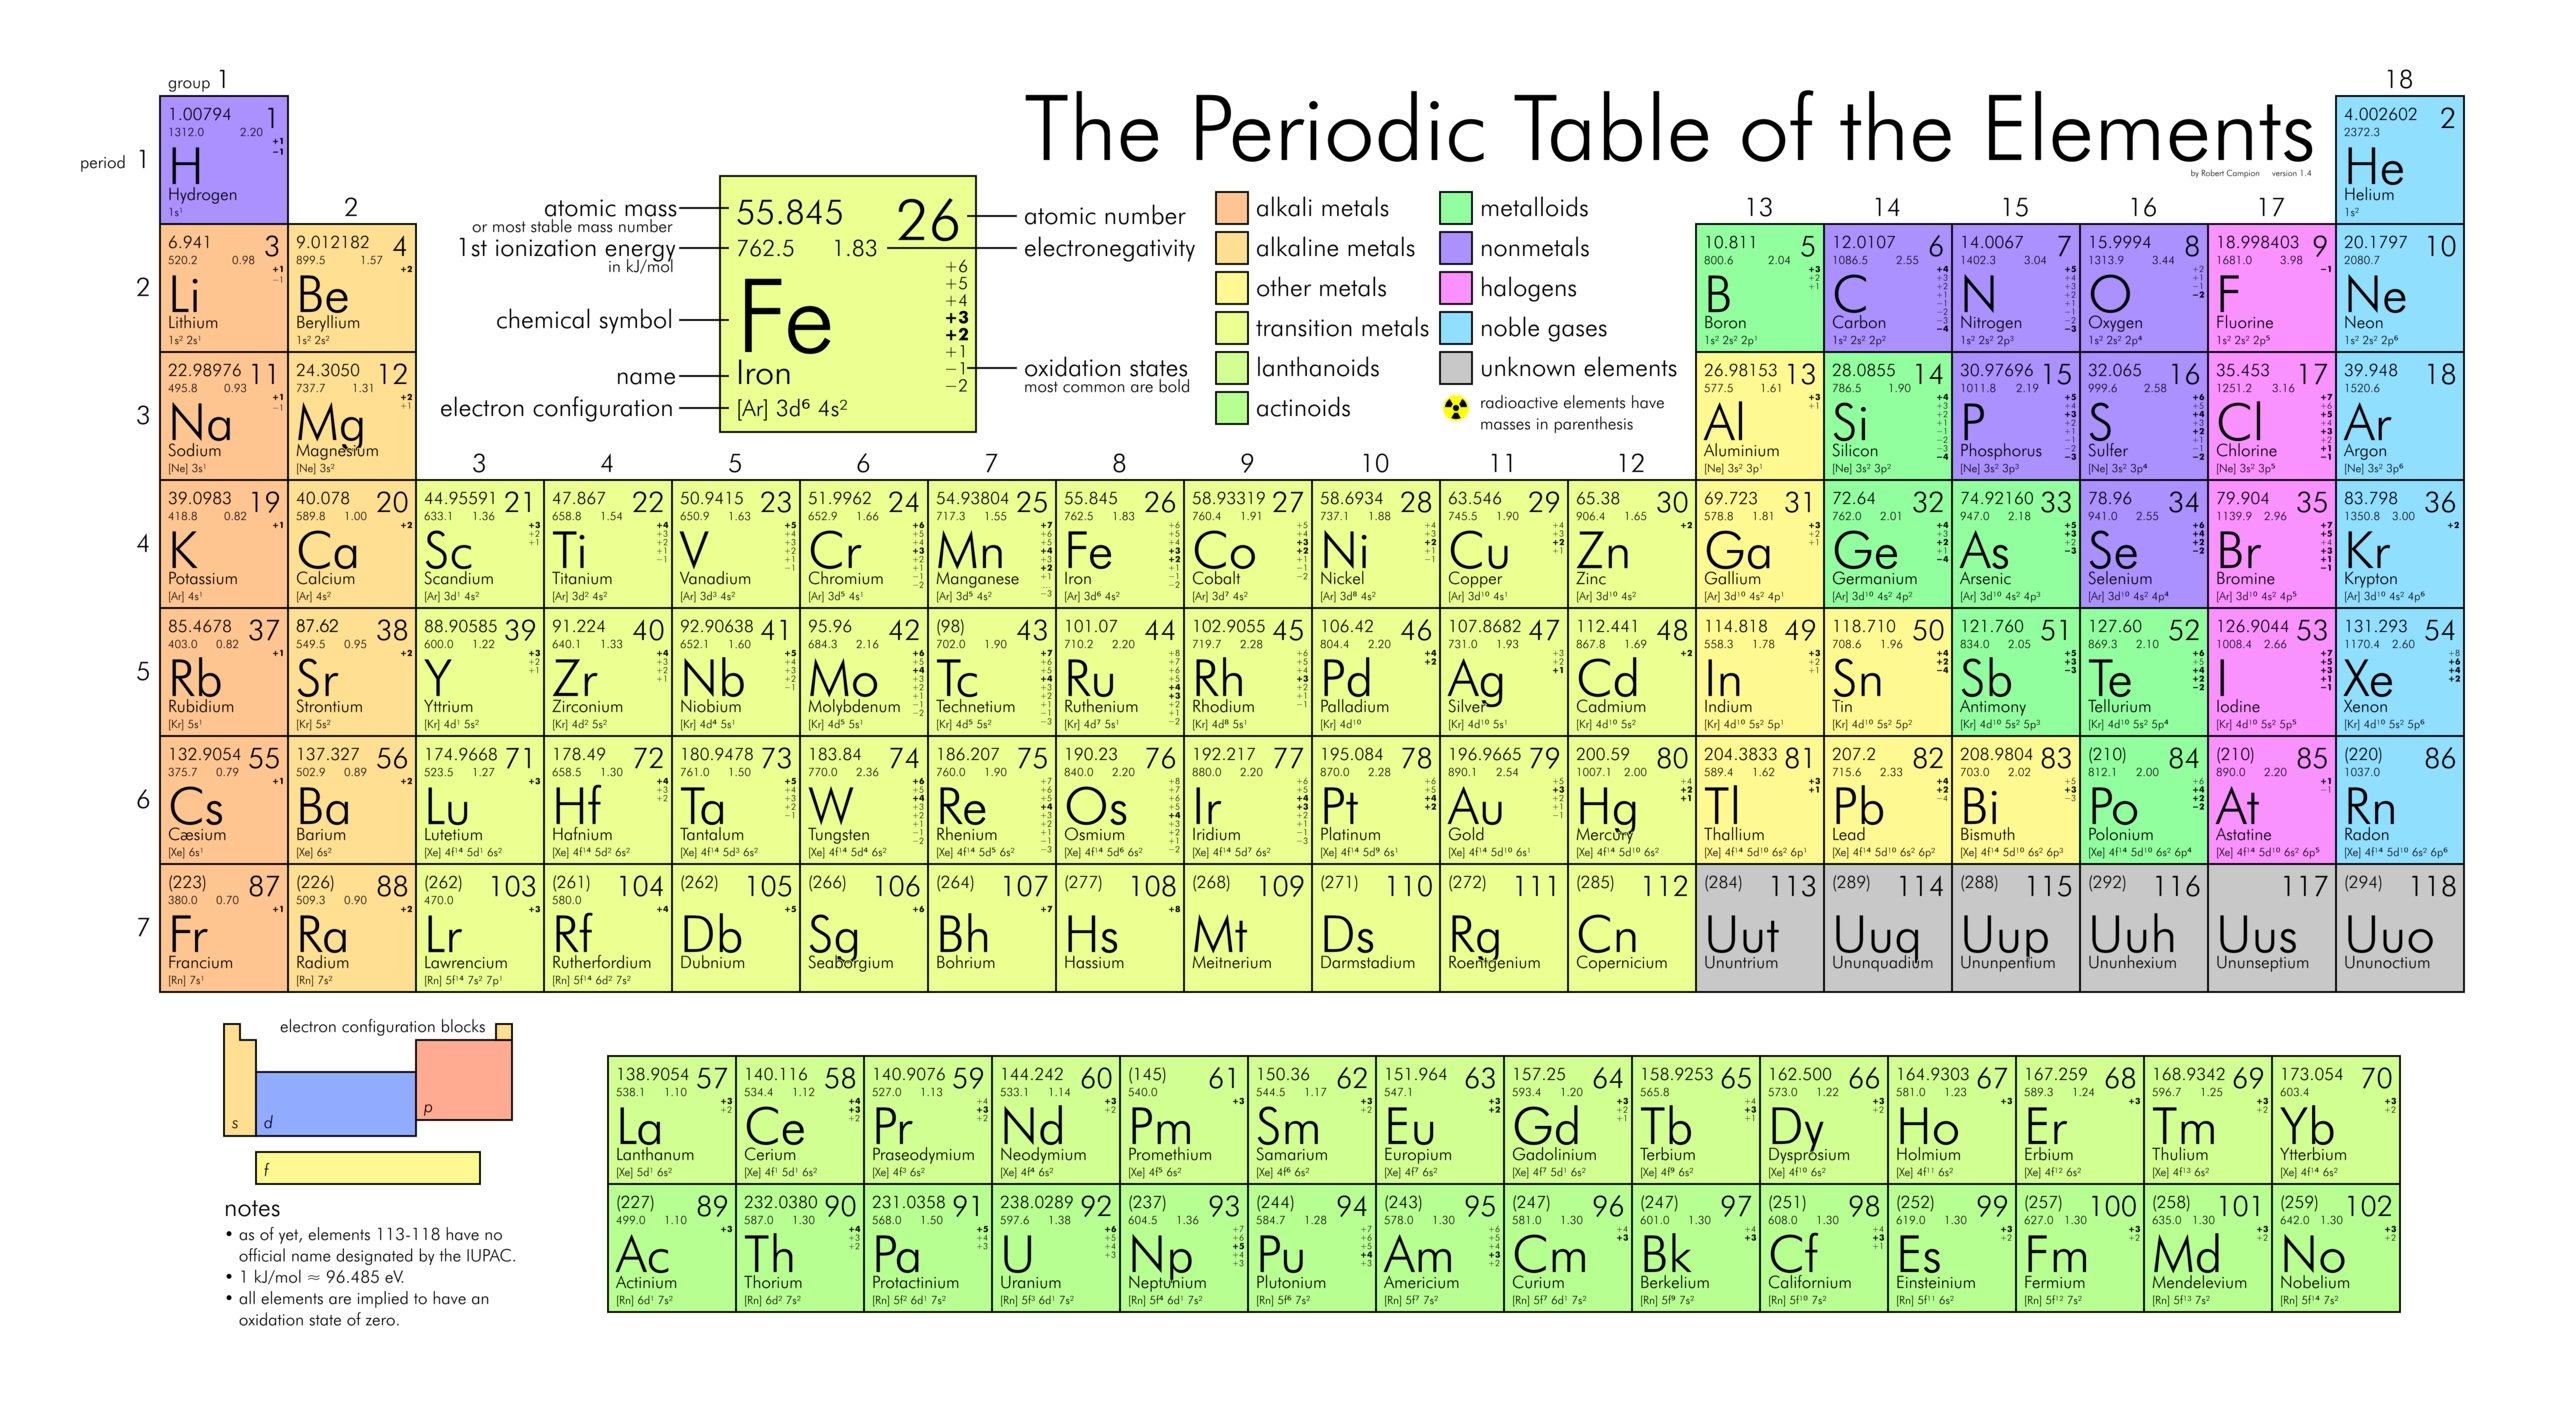
\includegraphics[width=0.75\textwidth]{periodic.png}
% ADD: Periodic Trends, Periods, Collums, Atomic Radius, Electronegativity,
% Image: https://sciencenotes.org/wp-content/uploads/2014/10/PeriodicTableTrends.png

\pagebreak
There is a square for each element. In the middle you see the atomic
symbol and the name of the element. In the upper right corner is the
atomic number -- the number of protons in the atom.

In the upper left corner is the atomic mass in atomic mass units.\index{atomic mass}
% Image: https://cdn.britannica.com/98/22298-050-A29636A6/properties-Nobelium.jpg

Look at the atomic mass of boron. About 80\% of all boron atoms have
six neutrons. The other 20\% have only 5 neutrons. So most boron atoms
have a mass of about 11 atomic mass units, but some have a mass of
about 10 atomic mass units. The atomic mass of boron is equivalent to the average
mass of a boron atom: 10.811.
% ADD: Talk about mass spectroscopy
% Image: https://cdn.kastatic.org/googleusercontent/EblyOpI1NnDQ3H9TDLERVAIt1Y9ZCDGOFJtd-lzQKNMJitDTQF-Yue-n6QNlzJvSyXeQfCe0YP6zm3tm4hDoGNwN

\begin{Exercise}[title={Mass of a Water Molecule}, label=water_mass]
  
Using the periodic table, what is the average mass of one water molecule in atomic mass units?

\end{Exercise}
\begin{Answer}[ref=water_mass]

  The average hydrogen atom has a mass of 1.00794 atomic mass units.

  The average oxygen atom has a mass of 15.9994.

  $2 \times 1.00794 + 15.9994 = 18.01528$ atomic mass units.
   
\end{Answer}

\section{Molar Mass}

An atomic mass unit is a very, very, very small unit; we would much
rather work in grams.  It turns out that $6.02214076 \times 10^{23}$
atoms equal 1 mole( a standard measure for chemistry). Scientists use this number so much
that they gave it a name: \textit{the Avogadro constant} or
\textit{Avogadro's number}.\index{Avogadro's number}
% KA: https://www.khanacademy.org/science/ap-chemistry-beta/x2eef969c74e0d802:atomic-structure-and-properties/x2eef969c74e0d802:moles-and-molar-mass/v/the-mole-and-avogadro-s-number

If you have 12 doughnuts, that's a dozen doughnuts.  If you have
$6.02214076 \times 10^{23}$ doughnuts, you have a \textit{mole} of
doughnuts. (Note: it isn't actully practical to measure doughnuts this
way: A mole of doughnuts would be about the size of the earth. We use
moles for small things like molecules.)\index{mole}

Let's say you want to know how much a mole of $NaCl$ weighs. From the
periodic table, you see that $Na$ has an atomic mass of 22.98976
atomic mass units. And $Cl$ has 35.453 atomic mass units.  One atom of
$NaCl$ has a mass of $22.98976 + 35.453 = 58.44276$ atomic mass units.
Then a mole of $NaCl$ has a mass of $58.44276$ grams. Handy, right?
% ADD: Conversions should probably come before this

\begin{Exercise}[title={Burning Methane}, label=burning_methane]
  
Natural gas is mostly methane ($CH_4$). When one molecule of methane
burns, two oxygen molecules ($O_2$) are consumed. One molecule of
$H_2O$ and one molecule of $CO_2$ are produced.
% ADD: Need to explain mole to mole ratios first, Law of Divine Proportion
% ADD: Include Significant Figures

If I need 200 grams of water, how many grams of methane do I need
to burn?

(This is how the hero in ``The Martian'' made water for his garden.)

\end{Exercise}
\begin{Answer}[ref=burning_methane]

From the last exercise, you know that 1 mole of water weighs 18.01528
grams. So 200 grams of water is about 11.1 moles. So you need to burn
11.1 moles of methane.

What does one mole of methane weigh? Using the periodic table:
$12.0107 + 4 \times 1.00794 = 16.04246$ grams.

$16.0424 \times 11.10 = 178.1$ grams of methane.
   
\end{Answer}

\section{Heavy atoms aren't stable}

When you look at the periodic table, there are a surpringly large
number of elements. You might be told to ``Drink milk so that you can
get the calcium you need.'' However, no one has told you ``You should
eat kale so that you get enough copernicium in diet.''

Copernicium, with 112 protons and 173 neutrons, has only been observed
 in a lab. It is highly radioactive and unstable(meaning it decays): a copernicium
atom usually lives for less than a minute before decaying.
% ADD: Half Life

The largest stable element is lead, which has 82 protons and between
122 and 126 neutrons. Elements with lower atomic numbers than lead,
have at least one stable isotope. Elements with higher atomic numbers
than lead don't.

Bismuth, with an atomic number of 83, is \textit{almost} stable. In fact, most
bismuth atoms will live for billions of years before decaying.

\chapter{Work and Energy}

In this chapter, we are going to talk about how engineers define work
and energy.  We have already talked about force. Force is measured in
newtons, and one newton is equal to the force necessary to accelerate one
kilogram at a rate of $1 m/s^2$.
% ADD: Format 1 m/s

When you lean on a wall, you are exerting a force on the wall, but you
aren't doing any work. On the otherhand, if you push a car for a mile,
you are clearly doing work. Work, to an engineer, is the force you
apply to something, aswell as the distance that it moves, in the direction
of the applied force. We measure work in \textit{joules}. A joule is one
newton of force over one meter.
% Image: 
For example, if you push a car uphill with a force of 10 newtons for 12
meters, you have done 120 joules of work.\index{work}
% ADD: We can represent this with the equations, Work Energy Therom

Work is how energy is transferred from one thing to another. When you
push the car, you also burn sugars(energy of the body) in your blood. That energy is then
transferred to the car: after it has been pushed uphill.

Thus, we measure the energy something consumes or generates in 
units of work: joules, killowatt hours, horsepower-hours, foot-pounds,
BTUs( British Thermal Unit), and calories.

Let's go over a few different forms that energy can take.
% KA: https://www.khanacademy.org/science/ms-physics/x1baed5db7c1bb50b:energy/x1baed5db7c1bb50b:changes-in-energy/a/changes-in-energy
\section{Heat}\index{heat}

When you heat something, you are transferring energy to it. The BTU
 is a common unit for heat: One BTU is the
amount of heat required to raise the temperature of one pound of water,
by one degree. One BTU is about 1,055 joules. In fact, when you buy and sell
natural gas as a fuel, it is priced by the BTU.\index{heat} \index{BTU}

\section{Electricity}\index{electricity}

Electricity is the movement of electrons. When you push electrons
through a space that resists their passage (like a light bulb),
energy is transferred from the power source ( a battery)
 into the source of the resistance.

Let's say your lightbulb consumes 60 watts of electricity, and you leave it on for 24 hours.
We would say that you have consumed 1.44 kilowatt hours or 3,600,000 joules.
% ADD: Explain conversion further or move conversion chapter up
% KA: https://www.khanacademy.org/science/in-in-class10th-physics/in-in-electricity/in-in-electric-current-circuit/v/intro-to-charge

\section{Chemical Energy}\index{chemical energy}

As mentioned early, some chemical reactions consume energy and some
produce energy. Thus, energy can be stored in the structure of a
molecule. When a plant uses photosynthesis to rearrange water and
carbon dioxide into a sugar molecule, it converts the energy in
the sunlight( solar energy) into chemical energy. Remember photosythesis is a process that releases energy.
Therefor, the sugar molecule has more chemical energy than the carbon dioxide and water molecules that were
used in its creation.
% ADD: photosythesis equation 
% KA: https://www.khanacademy.org/science/ap-biology/cellular-energetics/photosynthesis/a/intro-to-photosynthesis

In our diet, we measure this energy in \textit{kilocalories}. A
calorie is the energy necessary to raise one gram of water one degree
Celsius: it is about 4.19 joules. This is a very small unit: an apple
has about 100,000 calories( 100 kilocalories), so people working with food started
measuring everything in kilocalories.\index{calories}
% ADD: Conversion chapter should come before this chapter

Here is where things get confusing: People who work with food got tired of
saying ``kilocalories'', so they just started using ``Calorie'' to
mean 1,000 calories.  This has created terrible confusion over the
years. So if the C is capitalized, ``Calorie'' probably means kilocalorie.

\section{Kinetic Energy}\index{kinetic energy}

A mass in motion has energy. For example, if you are in a moving car
and you slam on the breaks, the energy from the motion of the
car will be converted into heat in the breaks and under the tires.

How much energy does the car have?
% ADD: section specifically about KE AND U, use roller coaster diagram

\begin{mdframed}[style=important, frametitle={Formula for Kinetic Energy}]

$$E = \frac{1}{2} m v^2$$

where $E$ is the energy in joules, $m$ is the mass in kilograms, and
$v$ is the speed in meters per second.

\end{mdframed}

\section{Gravitational Potential Energy}\index{potential energy!gravitational}
% KA: https://youtu.be/oGzwVYPxKjg

When you lift something heavy onto a shelf, you are giving it
\textit{potential energy}. The amount of energy that you transferred
to it is proportional to its weight and the height that you lifted it.

On the surface of the earth, gravity will accelerate a heavy objects downward at
a rate of $9.8 m/s^2$.

\begin{mdframed}[style=important, frametitle={Formula for Gravitational Potential Energy}]
On earth, then, gravitational potential energy is given by

$$E = (9.8)mh$$


where $E$ is the energy in joules, $m$ is the mass of the object you
lifted, and $h$ is the height that you lifted it.

\end{mdframed}


There are other kinds of potential energy. For example, when you draw
a bow, you have given that bow potential energy. When you release it,
the potential energy is transferred to the arrow, which expresses it
as kinetic energy.
% ADD: section about KE and U

\section{Conservation of Energy}

The first law of thermodynamics says ``Energy is neither created nor
destroyed.''\index{energy!conservation of}

Energy can change forms: Your cells consume chemical energy to give
gravitational potential energy a car you push up a hill. However, the total amount of
energy in a closed system stays constant.
% ADD: Create Systems chapter before introducing concept here

\begin{Exercise}[title={The Energy of Falling}, label=energy_falling]
  
A 5 kg cannonball falls off the top of a 3 meter ladder. Just before
it hits the floor, all of its gravitational potential energy has been
converted into kinetic energy.  How fast is the cannonball going when
it hits the floor?

\end{Exercise}
\begin{Answer}[ref=energy_falling]

  At the top of the ladder, the cannonball has $(9.8)(5)(3) = 147$ joules of potential energy.

  At the bottom, the kinetic energy $\frac{1}{2}(5)v^2$ must be equal
  to 147 joules. So $v^2 = \frac{294}{5}$.  Thus it is going about
  $7.7$ meters per second.

  (Yes, a tiny amount of energy is lost to air resistance. For a dense
  object moving at these relatively slow speeds, this energy is
  neglible.)
  
\end{Answer}


\section{Efficiency}
% KA: https://www.khanacademy.org/science/ap-biology/cellular-energetics/cellular-energy/a/the-laws-of-thermodynamics

Although energy is always conserved as it moves through different
forms, scientists aren't always that good at controlling it.\index{efficiency}

For example, a car engine consumes the chemical energy in gasoline. Only
about 20\% of the energy consumed is used to turn the wheels.  Most of
the energy is actually lost as heat. If you run a car for a while, the engine
gets very hot and the exhaust going out the tail pipe turns hot.

A human is about 25\% efficient. Most of the loss is in the heat produced
during the chemical reactions that turns food into motion.
% ADD: Cellular Respiration
 
In general, if you are trying to increase efficiency in any system,
the solution is usually easy to identify because heat is produced. Reduce heat, Increase efficiency.

Light bulbs are an interesting case. To get the light of a 60 watt
incandescent bulb, you can use an 8 watt LED or a 16 watt flourescent
light. Thus, we say that the LED light is much more efficient: If you
run both, the incandescent bulb will consume 1.44 kilowatt-hours. The
LED will consume only 0.192 kilowatt hours.

Besides light, the incandescent bulb is producing a lot of heat. If it
is inside your house, what happens to the heat? It warms your house.

In the winter, when you want light and heat, the incandescent bulb is
100\% efficient!

In the summer, if you are running the air conditioner, the
incandescent bulb is worse that just ``inefficent at making light'' --
it is actually counteracting the air conditioner! 

\section{Cognitive bias: Self-Serving Bias}

\newterm{Self-serving bias} is when you blame the situation for your
failures, but attribute your successes to your strengths.

For example, when asked ``Why did you lose the match?'' you are likely
to answer ``The referee wasn't fair.''  When you are asked ``Why did
you win the match?'' you are likely to answer ``Because I have been
training for weeks, and I was very focused.''

This bias tends to make us feel better about ourselves, but it makes it
diffcult for us to be objective about our strengths and weaknesses.


\chapter{Units and Conversions}

At this point, you are working with a lot of units: grams for weight,
joules for energy, newtons for force, meters for distance, seconds for
time, etc. For each type of measurement, there are several different
units; for example, distance can be measured in feet, miles,
and light-years.

For your reference, here is a table of equivalencies:

\begin{tabular}{r | l}
  \hline
  \multicolumn{2}{c}{\textbf{Distance}}\\
  1 mile & 1.6093 kilometers \\
  1 foot & 0.3048 meters \\
  1 inch & 2.54 centimeters \\
  1 light-year & $9.461 \times 10^{12}$ kilometers\\
  \hline
  \multicolumn{2}{c}{\textbf{Volume}}\\
  1 milliliter & 1 cubic centimeter \\
  1 quart & 0.9461 liters \\
  1 gallon & 3.7854 liters \\
  1 fluid ounce & 29.6 milliliters \\
  \hline
  \multicolumn{2}{c}{\textbf{Mass}}\\
  1 pound & 0.4535924 kilograms\\
  1 ounce & 0.4535924 grams\\
  1 metric ton & 1000 kilograms \\
  \hline
  \multicolumn{2}{c}{\textbf{Force}}\\
  1 newton & 1 kilogram meter per sec$^2$\\
  \hline
  \multicolumn{2}{c}{\textbf{Pressure}}\\
  1 pascal & 1 newton per square meter \\
  1 bar & 0.98692 atmosphere \\
  1 pound per square inch & 6897 pascals \\
  \hline
  \multicolumn{2}{c}{\textbf{Energy}}\\
  1 joule & 1 newton meter \\
  1 calorie & 4.184 joules \\
  1 kilowatt-hour & $3.6 \times 10^{6}$ joules  \\
\end{tabular}\index{units table}

(You don't need to memorize these! Just remember that this page is here.)

In the metric system, prefixes are often used to express a multiple. Here are the common prefixes:\index{metric system!prefixes}

\begin{tabular}{r | l}
giga  & $\times 10^{9}$\\
mega  & $\times 10^{6}$\\
kilo  & $\times 10^{3}$\\
milli  & $\div 10^{3}$\\
micro  & $\div 10^{6}$\\
nano  & $\div 10^{9}$\\
\end{tabular}

(These are worth memorizing.)

\section{Conversion Factors}

Here is a really handy trick to remembering how to do conversions
between units.\index{conversion factors}

Often, you will a table like the one above, and someone will ask you
``How many miles are in 0.23 light-years?''  You know that 1 mile = 1.6093
kilometers and that 1 light-year is $9.461 \times 10^{12}$ kilometers.
How do you do the conversion?

The trick is to treat the two parts of the equality as a fraction that equals 1.  That is, you think:

$$\frac{1 \text{ miles}}{1.6093 \text{ km}} = \frac{1.6093 \text{ km}}{1 \text{ miles}} = 1$$

and

$$\frac{1 \text{ light-years}}{9.461 \times 10^{12} \text{ km}} = \frac{9.461 \times 10^{12} \text{ km}}{1 \text{ light-years}} = 1$$

We call these fractions \textit{conversion factors}.

Now, your problem is

$$0.23 \text{ light-years} \times \textit{ Some conversion factors} = ? \text{ miles}$$

Note that when you multiply fractions together, things in the numerators can cancel with things in the denominator:

$$\left( \frac{31\pi}{47} \right) \left( \frac{11}{37\pi}\right) = \left(\frac{31\cancel{\pi}}{47}\right) \left( \frac{11}{37\cancel{\pi}}\right) = \left(\frac{31}{47} \right) \left( \frac{11}{37} \right)$$

When working with conversion factors, you will do the same with the units:

\begin{multline*}
  0.23 \text{ light-years} \left( \frac{9.461 \times 10^{12} \text{ km}}{1 \text{ light-years}} \right) \left( \frac{1 \text{ miles}}{1.6093 \text{ km}} \right) = \\
  0.23 \text{ \cancel{light-years}} \left( \times \frac{9.461 \times 10^{12} \text{ \cancel{km}}}{1 \text{ \cancel{light-years}}} \right) \left( \frac{1 \text{ miles}}{1.6093 \text{ \cancel{km}}}\right) = \frac{(0.23)(9.461 \times 10^{12})}{1.6093} \text{ miles}$$
\end{multline*}

\begin{Exercise}[title={Simple Conversion Factors}, label=simple_conversion_factors]

  How many calories are in 4.5 killowatt-hours?
  
\end{Exercise}
\begin{Answer}[ref=simple_conversion_factors]

  $$4.5 \text{ \cancel{kWh}} \left( \frac{3.6 \times 10^{6} \text{ \cancel{joules}}}{1 \text{ \cancel{kWh}}} \right) \left( \frac{1 \text{ calories}}{4.184 \text{ \cancel{joules}}}\right) = \frac{(4.5)(3.6 \times 10^6)}{4.184} = 1.08 \times 10^6 \text {calories}$$
  
\end{Answer}

\section{Conversion Factors and Ratios}

Conversion factors also work on ratios.  For example, if you are told
that a bug is moving 0.5 feet every 120 milliseconds. What is that in
meters per second?

The problem, then is

$$\frac{0.5 \text{ feet}}{120 \text{ milliseconds}} = \frac{\text{? m}}{second}$$

So you will need conversion factors to replace the ``feet'' with ``meters'' and to replace ``milliseconds'' with ``seconds'':

\begin{multline*}
\left(\frac{0.5 \text{ \cancel{feet}}}{120 \text{ \cancel{milliseconds}}}\right) \left( \frac{0.3048 \text{ meters}}{1 \text{ \cancel{feet}}} \right) \left( \frac{ 1000 \text{ \cancel{milliseconds}}} {1 \text{ second}}\right) = \frac{(0.5)(0.3048)(1000)}{120}\text{ m/second}
\end{multline*}

\begin{Exercise}[title={Conversion Factors}, label=conversion_factors]

The hole in the bottom of the boat lets in 0.1 gallons every 2 minutes.  How many milliliters per second is that?
  
\end{Exercise}
\begin{Answer}[ref=onversion_factors]

  \begin{multline*}
    \frac{0.1 \text{ \cancel{gallons}}}{2 \text{ \cancel{minutes}}}
  \left( \frac{3.7854 \text{ \cancel{liters}}}{1 \text{ \cancel{gallons}}} \right)
  \left( \frac{1000 \text{ milliliters}}{1\text{ \cancel{liters}}}\right)
  \left( \frac{1 \text{ \cancel{minutes}}}{60 \text{ seconds}} \right) = \\
  \frac{(0.1)(3.7854)(1000)}{(2)(60)} \text{ ml/second} = 3.1545 \text{ ml/second}
  \end{multline*}
  
\end{Answer}

\section{When Conversion Factors Don't Work}

Conversion factors only work when the units being converted are
proportional to each other. Gallons and liters, for example are
proportional to each other: If you have $n$ gallons, you have $n
\times 3.7854$ liters.

Degrees celsius and degrees farenheit are \textit{not} proportional to
each other.  If your food is $n$ degrees celsius, it is $n \times
\frac{9}{5} + 32$ degrees farenheit.  You can't use conversion factors
to convert celsius to farenheit.

\chapter{Simple Machines}

As mentioned earlier, physicists define work to be the force applied
times the distance it is applied over. So, if you pushed your car 100
meters with 17 newtons of force, you have done 1700 joules of work.

Humans have always had to move really heavy things, so many centuries
ago we developed simple machines to decrease the amount of force
necessary to execute those tasks. These include things like:
\begin{itemize}
\item Levers
\item Pulleys
\item Ramps
\item Gears
\item Hydraulics
\item Screws
\end{itemize}

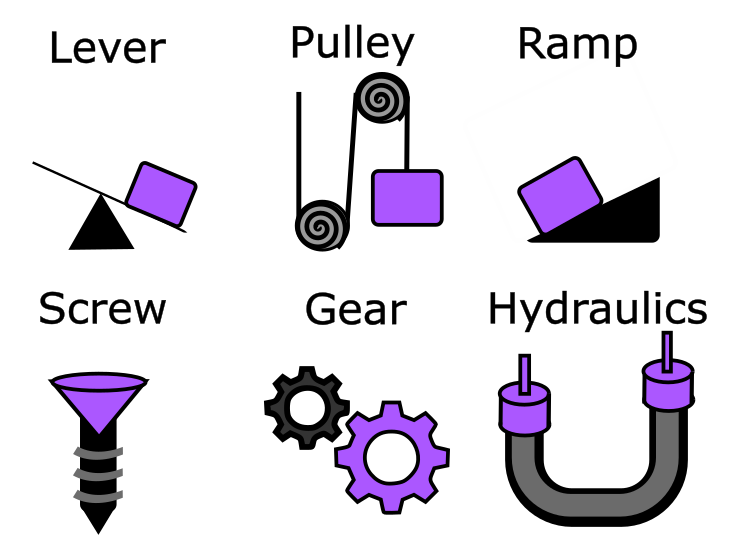
\includegraphics[width=0.8\textwidth]{Simple_Machines.png}

While these machines can decrease the force needed, they don't change
the amount of work that must be done. So if the force is decreased to
a third, the distance that you must apply the force is increased by a
factor of three.

``Mechanical gain'' is what we call the increase in force.

\section{Levers}

A lever rotates on a fulcrum. To decrease the necessary force, the load
is placed nearer to the fulcrum than where the force is applied.

In particular, physicists talk about the \newterm{torque} created by a
force. When you push on a lever, the torque is the product of the
force you exert and the distance from the point of rotation.

Torque is typically measured in newton-meters.

To balance two torques, the products must be the same. So, assuming
that the forces are applied in the proper direction,

$$R_L F_L = R_A F_A$$

where $R_L$ and $R_A$ are the distance from the fulcrum to the where
the load's force and the applied force (respectively) are applied, and
$F_L$ and $F_A$ are the amounts of the forces.

\begin{Exercise}[title={Lever}, label=lever]
  
Paul, who weighs 70 kilograms, sits on a see-saw 4 meters from the
fulcrum. Jan, who weighs 50 kilograms, wants to balance. How far
should Jan sit from the fulcrum?

\end{Exercise}
\begin{Answer}[ref=lever]
  Paul is exerting $(70)(9.8)$ newtons of force at 4 meters from the
  fulcrum, so he is creating a torque of 2,744 newton-meters of torque
  on the see-saw.  Jan is creating $(50)(9.5) = 490$ newtons of
  force.

  If $r$ is the distance from the fulcrum to Jan's seat, to balance
  $490 r = 2744$, so $r = 5.6$ meters.
\end{Answer}
% KA: https://www.khanacademy.org/science/physics/discoveries/simple-machines-explorations/a/lever

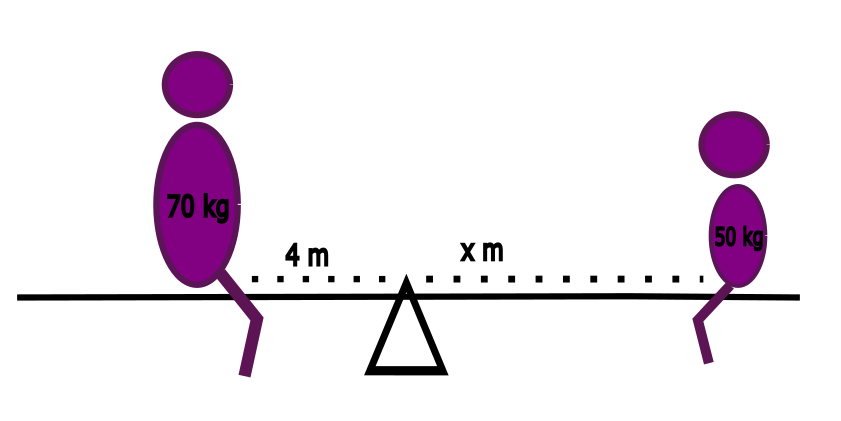
\includegraphics[width=0.8\textwidth]{fulcrum.png}

\section{Ramps}

Ramps, or incline planes, let you roll or slide objects up to a higher
level. Steeper ramps give you less mechanical gain. For example, it is much easier 
to roll a ball up a wheelchair ramp than on a skateboard ramp.
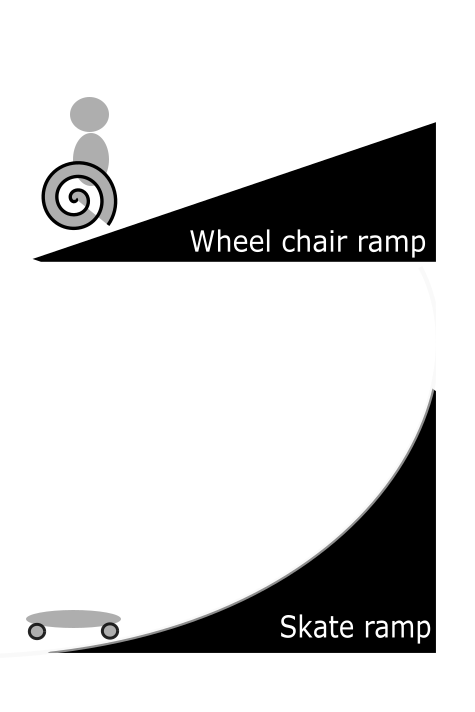
\includegraphics[width=0.8\textwidth]{ramps.png}

Assuming the ramp has a constant steepness, the mechanical gain is
equal to the ratio of the length of the ramp divided by the amount
that it rises.

If you assume there is no friction, the force that you push a weight up the ramp will be:

$$F_A = \frac{V}{L} F_G$$

Where $F_A$ is the force you need to push. $L$ is the length of the
ramp, $V$ is the amount of vertical gain and $F_G$ is the force of
gravity on the mass.

(We haven't talked about the sine function yet, but in case you already know about it: Note that

$$\frac{V}{L} = \sin{\theta}$$

where $\theta$ is the angle between the ramp and level.)

\begin{Exercise}[title={Ramp}, label=ramp]
A barrel of oil weighs 136 kilograms. You can push with a force of
up to 300 newtons. You have to get the barrel onto a platform that is 2
meters. What is the shortest board that you can use as a ramp?
\end{Exercise}
\begin{Answer}[ref=ramp]
  To lift the barrel would require $136 \times 9.8 = 1,332.8$ newtons of force.

  Letting $L$ be the length of the ramp:

  $$300= \frac{2}{L} 1332.8$$

  So $L = 8.885$ meters.
\end{Answer}

\section{Gears}

Gears (which might have a chain connecting them like on a bicycle)
have teeth and come in pairs. You apply torque to one gear, and it
applies torque to another. The torque is increased or decreased based
on the ratio between the teeth on the gears.


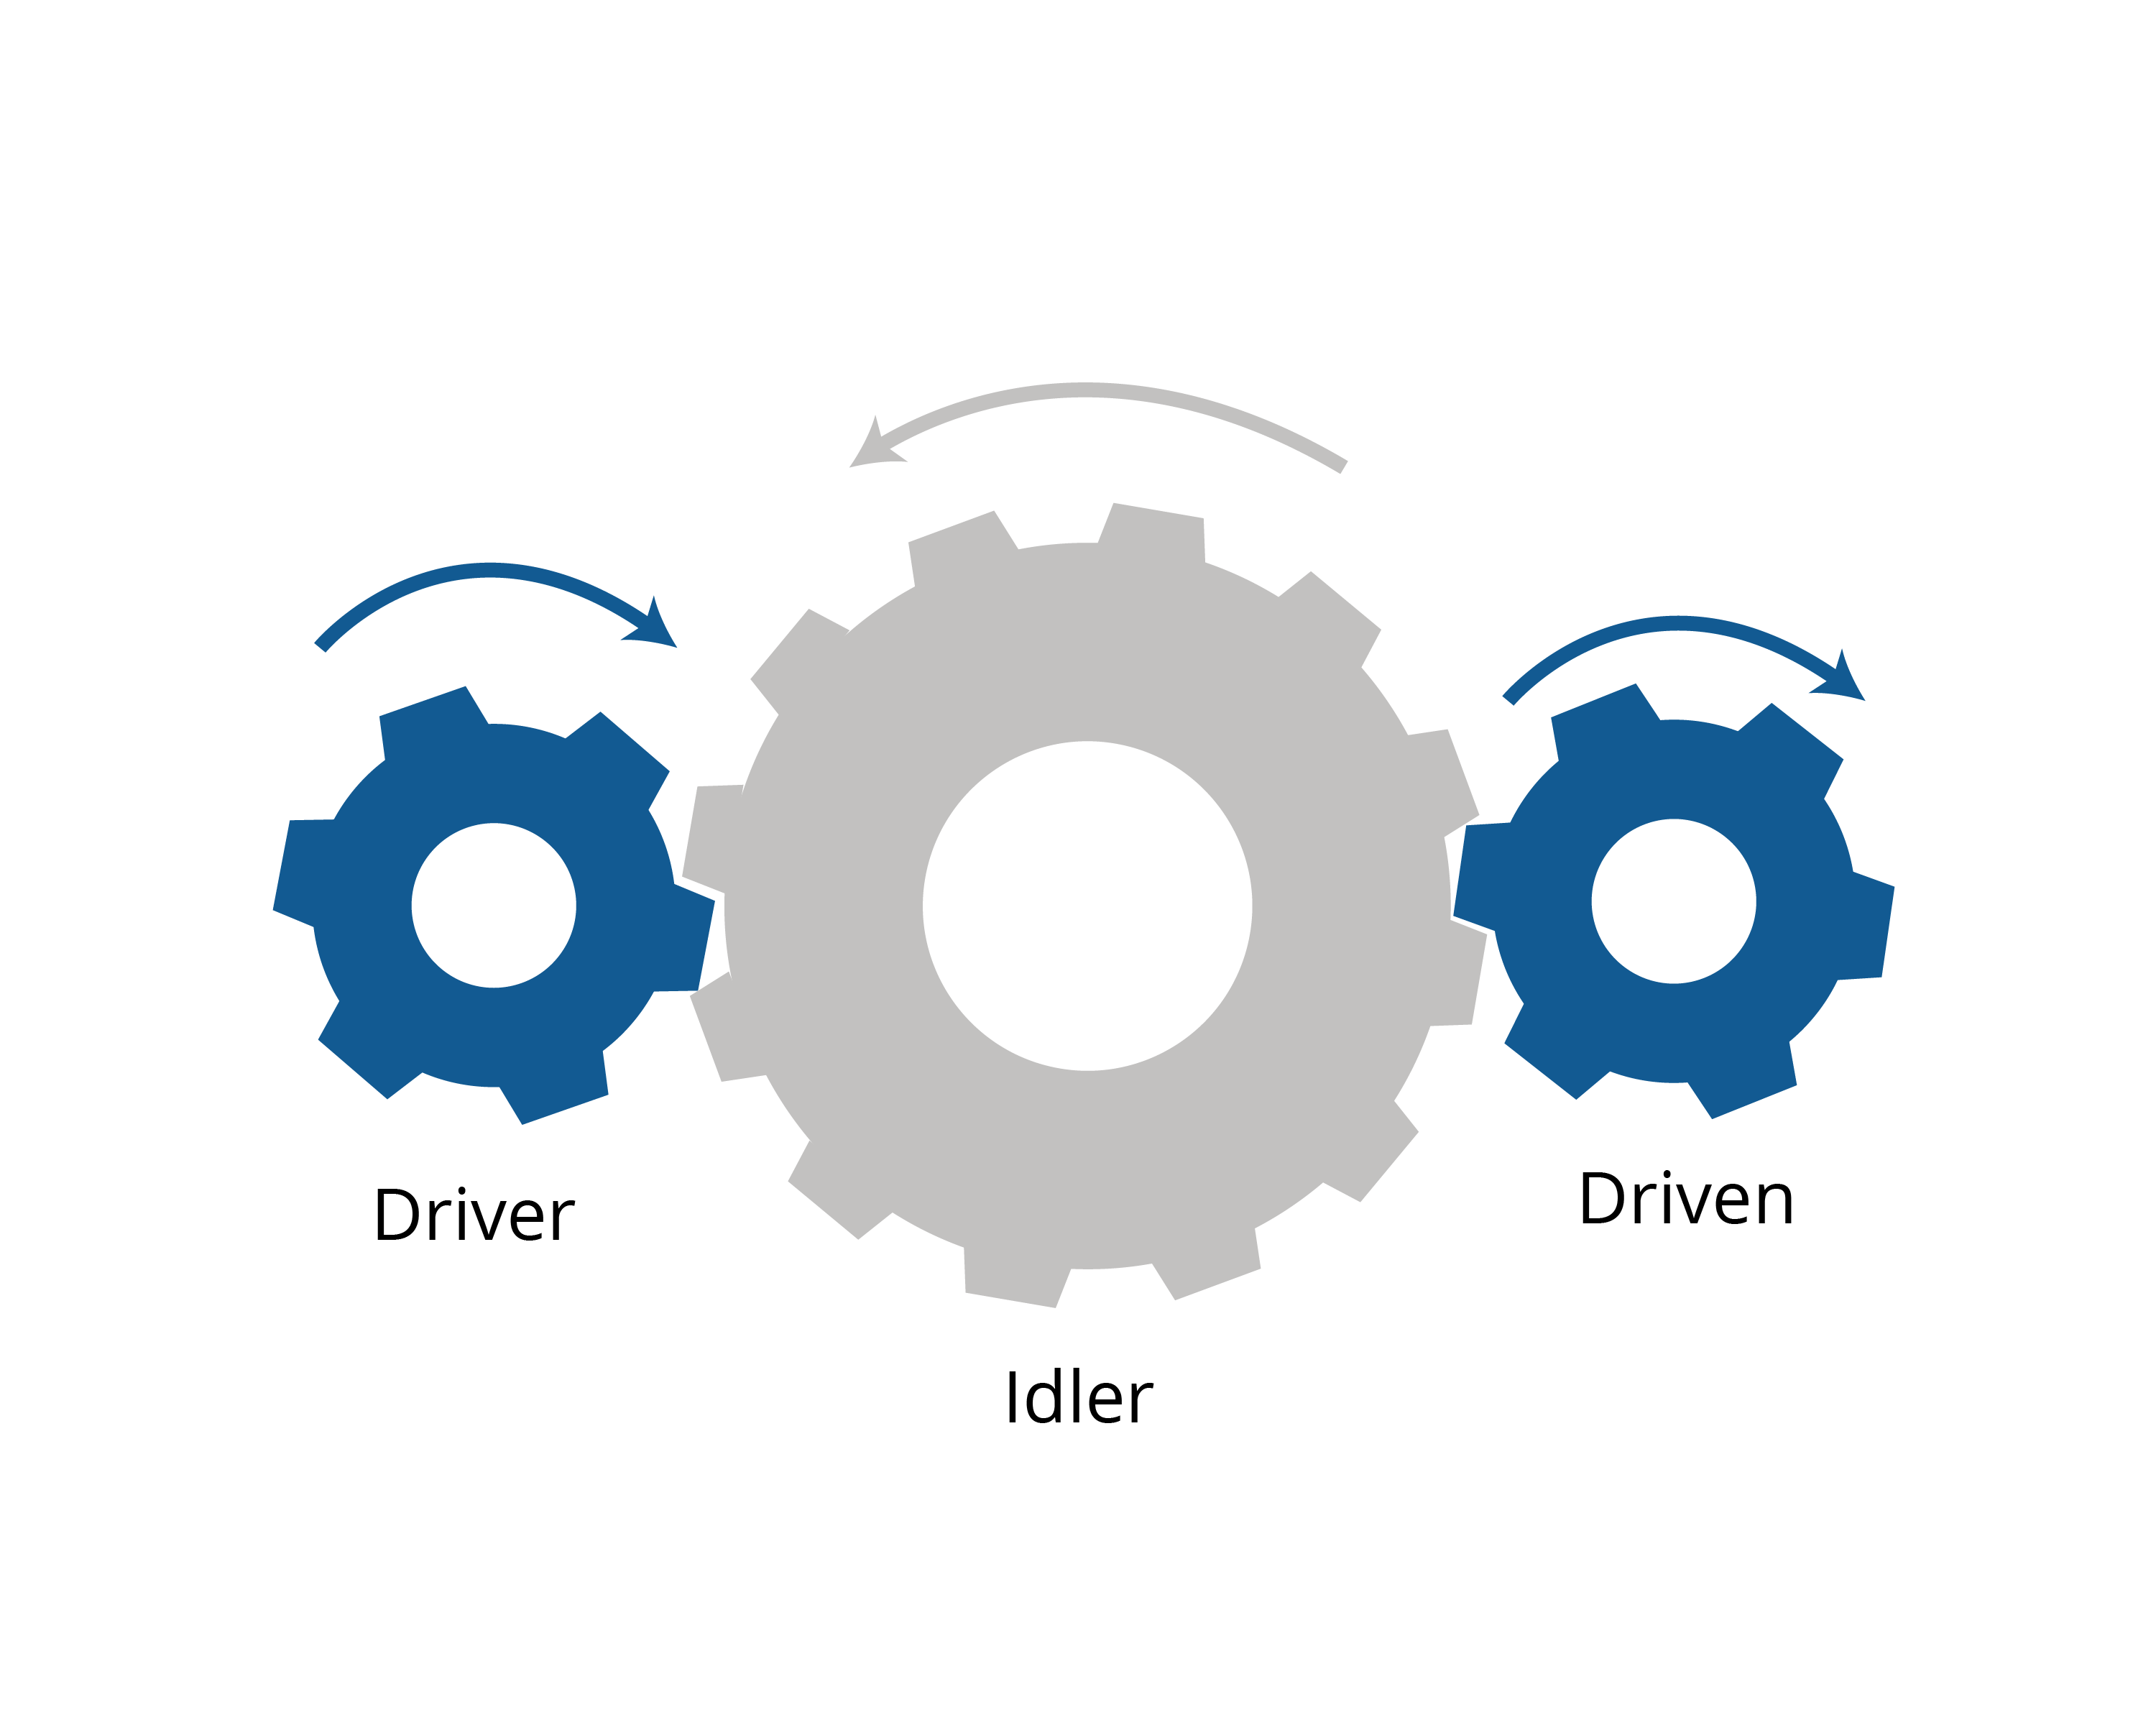
\includegraphics[width=0.8\textwidth]{Gears.png}


If $N_A$ is the number of teeth on the gear you are turning with a
torque of $T_A$, and $N_L$ is the number of teeth on the gear it is
turning, the resulting torque is:

$$T_L = \frac{N_A}{N_L} T_A$$


\begin{Exercise}[title={Gears}, label=gear]

The bicycle is an interesting case because we are not trying to get
mechanical gain. We want to spin the pedals slower with more force.
  
You like to pedal your bike at 70 revolutions per minute. The
chainring that is connected to your pedals has 53 teeth. The
circumference of your tire is 2.2 meters. You wish to ride a 583 meters
per minute.

How many teeth should the rear sprocket have?
  
\end{Exercise}
\begin{Answer}[ref=ramp]
  
  $$583 = (70)(2.2)\frac{53}{n}$$
  
Thus $n = 14$ teeth.
\end{Answer}
% KA: https://www.khanacademy.org/science/physics/discoveries/simple-machines-explorations/a/simple-machines-and-how-to-use-this-tutorial

\section{Hydraulics}

In a hydraulic system, like the braking system of a car, you exert
force on a piston filled with fluid. The fluid carries that pressure
into another cylinder. The pressure of the fluid pushes the piston in
that cylinder out.

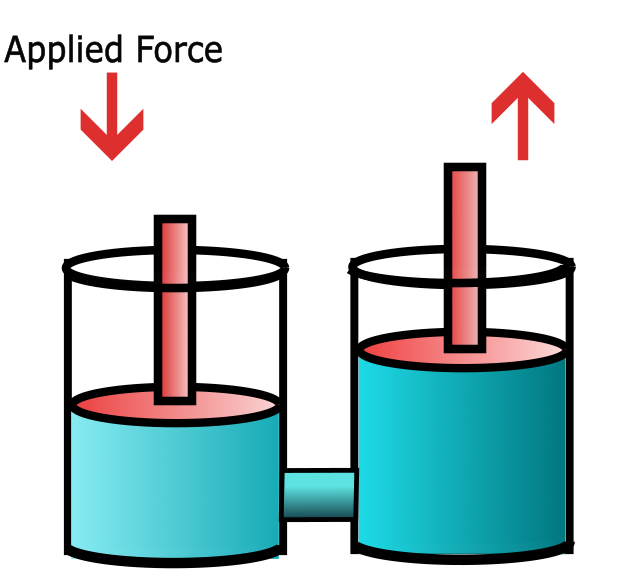
\includegraphics[width=0.8\textwidth]{hydraulics.png}


The pressure in the hose can be measured in pounds per square inch
(PSI) or newtons per square meter (Pascals or Pa). We will use Pascals.
% ADD: Create a page in the back of the book with units

To figure out how much pressure you create, you divide the force by
the area of the piston head you are pushing.

To figure out how much force that creates on the other end, you
multiply the pressure times the area of the piston head that is
pushing the load.

\begin{Exercise}[title={Hydraulics}, label=hydraulics]

Your car has disc brakes. When you put 2,500,000 pascals of pressure on the
brake fluid, the car stops quickly. As the car designer, you would like
that to require 12 newtons of force from the driver's foot.

What should the radius of the master cylinder (the one the driver is pushing on) be?
\end{Exercise}
\begin{Answer}[ref=hydraulics]
  We are looking for $r$, the radius of the piston head in meters. The area of the piston head is $\pi r^2$.

  The pressure in pascals of the brake fluid is given by $12 / (\pi r^2)$.

  $$2,500,000 = \frac{12}{\pi r^2}$$

  So $r = \sqrt{\frac{12}{\pi \times 2.5 \times 10^6}} = 0.001236077446474$ meters.

\end{Answer}
% KA: https://youtu.be/Pn5YEMwQb4Y



\chapter{Heat}

Let's say you put a 1 kg aluminum pan that is $80^\circ$ C into
3 liters of water that is $20^\circ$ C. Energy, in the form of heat,
will be transferred from the pan to the water until they are at the same
temperature. (We call this ``thermal equilibrium.'')\index{thermal equilibrium}

What will the temperature of the water be?

\section{Specific Heat Capacity}

If you are heating something, the amount of energy you need to
transfer to it depends on three things: the mass of the thing you are
heating, the amount of temperature change you want, and the
\textit{specific heat capacity} of that substance.\index{specific heat capacity}

\begin{mdframed}[style=important, frametitle={Energy in Heat Transfer}]

  The energy moved in a heat transfer is given by

  $$E = m c \Delta_T$$

  where $m$ is the mass, $\Delta_T$ is the change in temperature, and
  $c$ is the specific heat capacity of the substance.
% ADD: q=mcat

  (Note that this
  assumes no phase change. For example, this formula works nicely on
  warming liquid water, but it gets more complicated if you warm the
  water past its boiling point.)

\end{mdframed}

Can we guess the specific heat capacity of a substance? It is very,
very difficult to guess the specific heat of a substance, so we determine
it by experimentation.

For example, someone determined that it took about 0.9 joules to raise
the temperature of solid aluminum one degree Celsius. So we say ``The
specific heat capacity of aluminum is 0.9 J/g $^\circ$C.''

The specific heat capacity of liquid water is about 4.2 J/g $^\circ$C.

To answer the question, then, the amount of energy given off by the
pan must equal the amount of energy absorbed by the water. And they
need to be the same temperature at the end.  Let $T$ be the final
temperature of both.

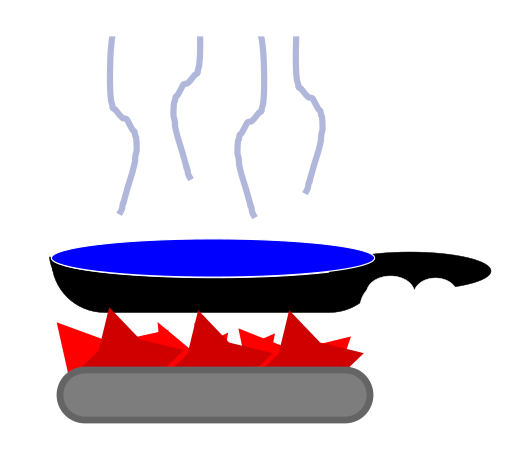
\includegraphics[width=0.8\textwidth]{Specific_Heat_Diagram.png}

% KA: https://www.khanacademy.org/science/ap-chemistry-beta/x2eef969c74e0d802:thermodynamics/x2eef969c74e0d802:heat-capacity-and-calorimetry/v/heat-capacity


Three liters of water weighs 3,000 grams, so the
change in energy in the water will be:

$$E_W = m c \Delta_T = (3000)(4.2)(T - 20) = 12600T - 252000 \text{ joules}$$ 

The pan weighs 1000 grams, so the change in energy in the pan will be::

$$E_P = m c \Delta_T = (1000)(0.9)(T - 80) = 900T - 72000 \text{ joules}$$

Total energy stays the same so $E_W + E_P = 0$.  So you need to solve

$$(12600T - 252000) + (900T - 72000) = 0$$

And find that the temperature at equilibrium will be

$$T = 24^\circ \text{C}$$

\begin{Exercise}[title={Thermal Equilibrium}, label=thermal_equilibrium]

Just as you put the aluminium pan in the water as described above,
someone also puts a 1.2 kg block of copper cooled to 10 $^\circ$ C.
The specific heat of solid copper is about 0.4 J/g $^\circ$C.

What is the new temperature at equilibrium?

\end{Exercise}
\begin{Answer}[ref=thermal_equilibrium]

  $$E_C = (1200)(0.4)(T - 10) = 480T - 4800$$

Total energy stays constant:

$$0 = (12600T - 252000) + (900T - 72000) + (480T - 4800)$$

Solving for $T$ gets you $T = 23.52^\circ$ C.

\end{Answer}

\section{Getting to Equilibrium}

When two objects with different temperatures are touching, the speed
at which they exchange heat is proportional to the differences in
their temperatures. Thus, as their temperatures get closer together,
the heat exchange slows down.
% ADD: explain which object, water or metal has a greater tempature change

In our example, the pan and the water will get close to equilibrium
quickly, but they may never actually reach equilibrium.

\begin{tikzpicture}
    \begin{axis}[
        xmin=0,xmax=4.25,
        ymin=15,ymax=85,
        axis x line=middle,
        axis y line=middle,
        axis line style=<->,
        xlabel={minutes},
        ylabel={degrees celsius},
        ]
        \addplot[no marks,sdkblue] expression[domain=0:4,samples=100]{24 + 56 * pow(2,-1.5 * x)} node[above, xshift=-1cm, yshift=0.1cm]{Pan}; 
        \addplot[no marks,sdkblue] expression[domain=0:4,samples=100]{24 - 4 * pow(2,-0.8 * x)} node[below, xshift=-2.5cm]{Water};
        \addplot[no marks,dashed,gray] coordinates {(0,24)(6,24)} node[above, xshift=-8cm]{equilibrium};
    \end{axis}
\end{tikzpicture}

\begin{Exercise}[title={Cooling Your Coffee}, label=cool_coffee]

  You have been given a ridiculously hot cup of coffee and a small pitcher of chilled milk.

  You need to start chugging your coffee in three minutes, and you want it as cool as possible at that time. When should you add the milk to the coffee?

\end{Exercise}
\begin{Answer}[ref=cool_coffee]

  During the 3 minutes, you want the coffee to give off as much of its
  heat as possible, so you want to maximize the difference between the
  temperature of the coffee and the temperature of the room around
  it.

  You wait until the last moment to put the milk in.

\end{Answer}

\section{Specific Heat Capacity Details}

For any given substance, the specific heat capacity often changes a
lot when the substance changes state. For example, ice is 2.1 J/g
$^\circ$C, whereas liquid water is 4.2 J/g$^\circ$C.
% KA: https://www.khanacademy.org/science/biology/water-acids-and-bases/water-as-a-solid-liquid-and-gas/v/specific-heat-of-water

Even within a given state, the specific heat capacity varies a bit
based on the temperature and pressure. If you are trying to do these
sorts of calculations with great accuracy, you will want to find the
specific heat capacity that matches your situation. For example, I
might look for the specific heat capacity for water at $22^\circ$C at
1 atmosphere of pressure( atm).


\chapter{Basic Statistics}

You live near a freeway, and someone asks you, ``How fast do cars on that freeway drive?''

You say ``Pretty fast.''

And they say, ``Can you be more specific?''

And you point your radar gun at a car, and say ``That one is going 32.131 meters per second.''

And they say, ``I don't want to know about that specific car. I want to know about all the cars.''

So, you spend the day beside the freeway measuring the speed of every
car that goes by. And you get a list of a thousand numbers. Here is part of the
list:

\begin{tabular}{c | c | c}
30.462 m/s  & 29.550 m/s & 29.227 m/s \\
37.661 m/s  & 27.899 m/s & 28.113 m/s \\
24.382 m/s & 35.668 m/s & 43.797 m/s \\
31.312 m/s & 37.637 m/s & 30.891 m/s
\end {tabular}

There are 12 numbers here. We say that there are 12 \textit{samples}.\index{samples}

\section{Mean}

We often talk about the \textit{average} of a set of samples, which is the 
same as the \textit{mean}. To get the mean, sum up the
samples and divide that number by the number of samples.\index{mean}

The numbers in that table sum to $388.599$.  If you divide that by 12,
you find that the mean of those samples is 32.217 m/s.

We typically use the greek letter $\mu$ (``mu'') to represent the mean.

\begin{mdframed}[style=important, frametitle={Definition of Mean}]
  
If you have a set of samples $x_1, x_2, \ldots, x_n$, the mean is:

$$ \mu = \frac{1}{n} \sum_{i=1}^n x_i$$

\end{mdframed}

This may be the first time you are seeing a summation ($\sum$). The equation above is equivalent to:\index{summation symbol}

$$ \mu = \frac{1}{n} \left(x_1 + x_2 + \ldots + x_n\right)$$

\begin{Exercise}[title={Mean Grade}, label=grades_mean]

  Teachers often use the mean for grading. For example, if you took
  six quizzes in a class, your final grade might be the mean of the six
  scores. Find the mean of these six grades: 87, 91, 98, 65, 87, 100.

\end{Exercise}
\begin{Answer}[ref=grades_mean]

  $$\mu =\frac{1}{6} \left(87 + 91 + 98 + 65 + 87 + 100 \right) = 88$$

\end{Answer}

If you tell your friend ``I measured the speed of 1000 cars, and the
mean is 31.71 m/s'', your friend will wonder ``Are most of the speeds
clustered around 31.71? Or are they all over the place and just happen
to have a mean of 31.71?'' To answer this question we use variance.

\section{Variance}

\begin{mdframed}[style=important, frametitle={Definition of Variance}]

If you have $n$ samples $x_1, x_2, \ldots, x_n$ that have a mean of $\mu$, the \textit{variance} is defined to be:\index{variance}

$$v = \frac{1}{n}\sum_{i = 1}^{n} \left(x_i - \mu\right)^2$$
% ADD: Maybe connect to Chi-squared test
\end{mdframed}

That is, you figure out how far each sample is from the median, you
square that, and then you take the mean of all those squared
distances.

\begin{tabular} {c | c | c}

  $x$ & $x - \mu$ & $(x - \mu)^2$\\
  \hline
30.462 & -1.755 & 3.079 \\
29.550 & -2.667 & 7.111\\
29.227 & -2.990 & 8.938\\
37.661 & 5.444 & 29.642\\
27.899 & -4.318 & 18.642\\
28.113 & -4.104 & 16.839 \\
24.382 & -7.835 & 61.381 \\
35.668 & 3.451 & 11.912 \\
43.797 & 11.580 & 134.106\\
31.312 & -0.905 & 0.818\\
37.637 & 5.420 & 29.381\\
30.891 & -1.326 & 1.757\\
\hline
$\sum x = 386.599$ & & $\sum (x - \mu)^2 = 323.605$\\
mean = 32.217 & & variance = 26.967
\end{tabular}

Thus, the variance of the 12 samples is 26.967. The bigger the variances, 
the farther the samples are spread apart; the smaller the variances, the closer
samples are clustered around the mean.

Notice that most of the data points deviate from the mu by 1 to 5
m/s. Isn't it odd that the variance is a big number like 26.967?
Remember that it represents the average of the squares. Sometimes, to
get a better feel for how far the samples are from the mean, we use
the square root of the variance, which is called \textit{the standard
  deviation}.

The standard deviation of your 12 samples would be $\sqrt{26.9677} =
  5.193$ m/s.
% ADD: Bell curve, KA: https://www.khanacademy.org/computer-programming/spin-off-of-galton-board-exploration/1930953307/embedded?embed=yes&article=yes&editor=no&buttons=no&author=no&width=400&height=400

The standard deviation is used to figure out a data point is an
outlier. For example, if you are asked``That car that just sped
past. Was it going freakishly fast?'' You might respond, ``No, it was
within a standard deviation of the mean.'' or ``Yes, it's speed was 2
standard deviations more than the mean. They will probably get a ticket.''
% ADD: Box and whiskers plot?

A singular $\mu$ usually represents the mean. $\sigma$ usually represents
the standard deviation. So $\sigma^2$ represents the variance.

\begin{Exercise}[title={Variance of Grades}, label=grades_variance]

  Now find the variance for your six grades. As a reminder, they were: 87, 91, 98, 65, 87, 100.

  What is your standard deviation?

\end{Exercise}
\begin{Answer}[ref=grades_variance]

  The mean of your grades is $88$.

  The variance, then is

  $$\sigma^2 = \frac{1}{6} \left((87 - 88)^2 + (91 - 88)^2 + (98 - 88)^2 + (61 - 88)^2 + (87 - 88)^2 + (100 - 88)^2 \right) = \frac{784}{6} = 65 \frac{1}{3}$$

  The standard deviation is the square root of that: $\sigma = 8.083$ points.
  
\end{Answer}


\section{Median}

Sometimes you want to know where the middle is. For example, you want
to know the speed at which half the cars are going faster and half are
going slower. To get the median, you sort your samples from smallest
to largest. If you have an odd number of samples, the one in the
middle is the median. If you have an even number of samples, we take
the mean of the two numbers in the middle.\index{median}
% KA: https://www.khanacademy.org/math/cc-sixth-grade-math/cc-6th-data-statistics/mean-and-median/v/statistics-intro-mean-median-and-mode

In our example, you would sort your numbers and find the two in the middle:

\begin{tabular}{c}
24.382\\
27.899\\
28.113\\
29.227\\
29.550\\
\hline
\textbf{30.462}\\
\textbf{30.891}\\
\hline 
31.312\\
35.668\\
37.637\\
37.661\\
43.797\\
\end{tabular}

You take the mean of the two middle numbers: $(30.462 + 30.891)/2 =
30.692$.  The median speed would be 30.692 m/s.

Medians are often used when a small number of outliers majorly skew the
mean. For example, income statistics usually use the median income
because a few hundred billionares raise the mean a lot.

\begin{Exercise}[title={Median Grade}, label=grades_median]

  Find the median of your six grades: 87, 91, 98, 65, 87, 100.

\end{Exercise}
\begin{Answer}[ref=grades_median]

  In order the grades are 65, 87, 87, 91, 98, 100.  The middle two are 87
  and 91. The mean of those is 89. (Speed trick: The mean of two numbers is the
  number that is half-way between.)
  
 \end{Answer}


\section{Histograms}

A histogram is a bar chart that shows how many samples are in each
group. In our example, we group cars by speed. Maybe we count the
number of cars going between 30 and 32 m/s.  And then we count the
cars going between 32 and 34 m/2. And then we make a bar chart from
that data.\index{histograms}
% ADD: Have not explained histograms yet

Your 1000 cars would break up into these groups:

\begin{tabular}{ c | c }
0 - 2 m/s & 0 cars \\
2 - 4 m/s & 0 cars \\
4 - 6 m/s & 0 cars \\
\ldots & \ldots \\
20 - 22 m/s & 0 cars \\
22 - 24 m/s & 0 cars \\
24 - 26 m/s & 65 cars \\
26 - 28 m/s & 160 cars \\
28 - 30 m/s & 175 cars \\
30 - 32 m/s & 168 cars \\
32 - 34 m/s & 150 cars \\
34 - 36 m/s & 114 cars \\
36 - 38 m/s & 79 cars \\
38 - 40 m/s & 52 cars \\
40 - 42 m/s & 20 cars \\
42 - 44 m/s & 12 cars \\
44 - 46 m/s & 4 cars \\
46 - 48 m/s & 1 cars \\
48 - 50 m/s & 0 cars \\
\end{tabular}

Now we make a bar chart from that:

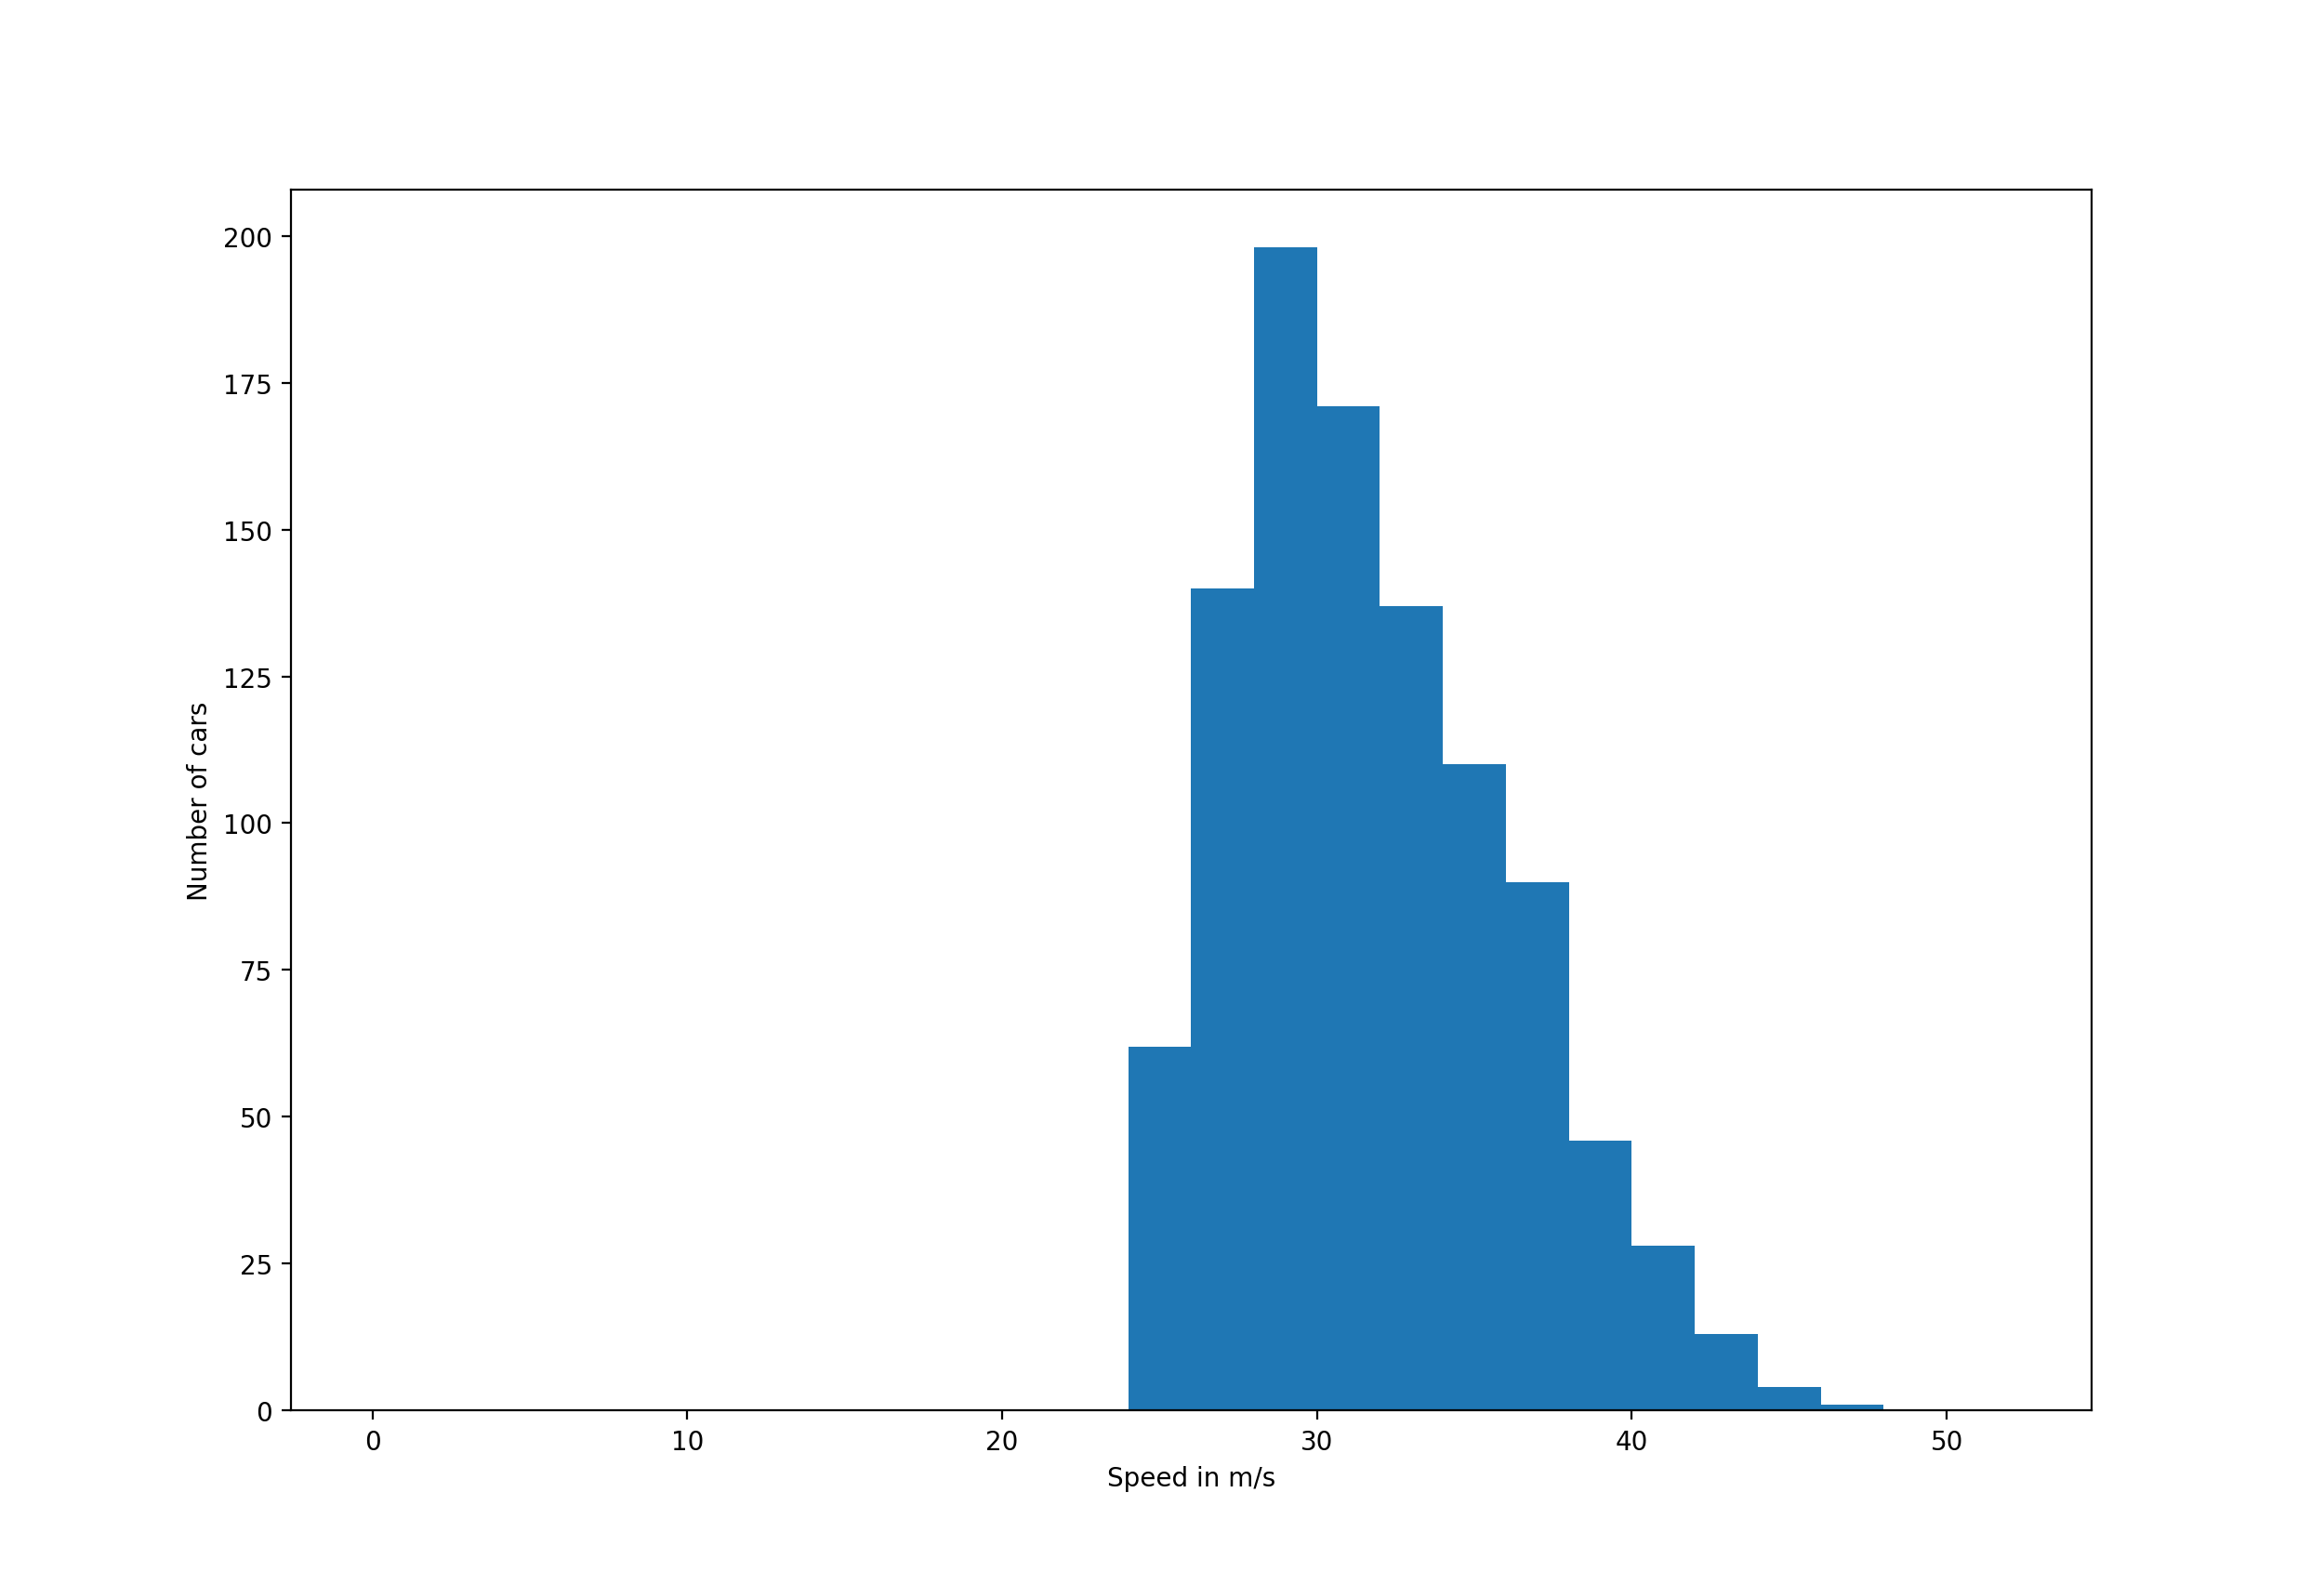
\includegraphics[width=\textwidth] {speed_histo.png}

Often a histogram will tell the story of the data. Here, you can see
that no one is going less than 24 m/s, but a lot of people travel at
30 m/s. There are a few people who travel over 40 m/s, but there are also a
couple of people who drive a lot faster than anyone else.

\section{Root-Mean-Squared}

Scientists have a mean-like statistic that they love. It is named
quadratic mean, but most just calls it Root-Mean-Squared or
RMS.

\begin{mdframed}[style=important, frametitle={Definition of RMS}]

If you have a list of numbers $x_1, x_2, \ldots, x_n$, their RMS
is \index{quadratic mean} \index{root-mean-squared} \index{RMS}

$$\sqrt{\frac{1}{n}\left( x_1^2 + x_2^2 + \ldots + x_n^2 \right)}$$

\end{mdframed}

You are taking the square root of the mean of squares of the samples,
thus the name Root-Mean-Squared.

Using your 12 samples:

\begin{tabular}{c |  c}
  $x$ & $x^2$ \\
  \hline
30.462 & 927.933 \\
29.550 & 873.203\\
29.227 & 854.218\\
37.661 & 1418.351\\
27.899 & 778.354\\
28.113 & 790.341\\
24.382 & 594.482\\
35.668 & 1272.206\\
43.797 & 1918.177\\
31.312 & 980.441\\
37.637 & 1416.544\\
30.891 & 954.254\\
\hline
\multicolumn{1}{r}{Mean of $x^2$} & {1064.875}\\
\multicolumn{1}{r}{RMS} & {32.632}
  \end{tabular}

Why is RMS useful? Let's say that all cars had the same mass $m$, and
you need to know what the average kinetic energy per car is. If you
know the RMS of the speeds of the cars is $v_{rms}$, the average kinetic energy for
each car is

$$k = \frac{1}{2}m v_{rms}^2$$

(You don't believe me? Let's prove it. Substitute in the RMS:

$$k = \frac{1}{2}m \sqrt{\frac{1}{n}\left( x_1^2 + x_2^2 + \ldots + x_n^2 \right)}^2$$

The square root and the square cancel each other out:

$$k = \frac{1}{2}m \frac{1}{n}\left( x_1^2 + x_2^2 + \ldots + x_n^2 \right)$$

Use the distributive property:

$$k = \frac{1}{n} \left( \frac{1}{2} m x_1^2 + \frac{1}{2}m x_2^2 + \ldots + \frac{1}{2}m x_n^2 \right)$$


That is all the kinetic energy divided by the number of cars, which is
the mean kinetic enegy per car. Quod erat demonstrandum! (That is a
Latin phrase that means ``which is what I was trying to
demonstrate''. You will sometimes see ``QED'' at the end of a long
mathematic proof.))

Now you are ready for the punchline: kinetic energy and heat are the
same thing. Instead of cars, heat is the kinetic energy of molecules
moving around. More on this soon.

Video: Mean, Median, Mode: https://www.youtube.com/watch?v=5C9LBF3b65s
\chapter{Basic Statistics in Spreadsheets}

When you completed the problems in the last section, you probably noticed
how long it took to compute statistics like the mean, the median,
and variance by hand. Luckliy, computers were designed to free us from these
sorts of tedious tasks. The most basic tool for automating
calculations is the spreadsheet program.\index{spreadsheet}

There are lots of spreadsheet programs including Microsoft's Excel and
Apple's Numbers. Any spreadsheet program will work; they are all very
similar. The instructions and screenshots here will be from Google
Sheets -- a free spreadsheet program you use through your web browser.

\section{Your First Spreadsheet}

In whatever spreadsheet program you are using, create a new spreadsheet document.

A spreadsheet is essentially a grid of cells. In each cell you can put data (like numbers or text) and a formulas.

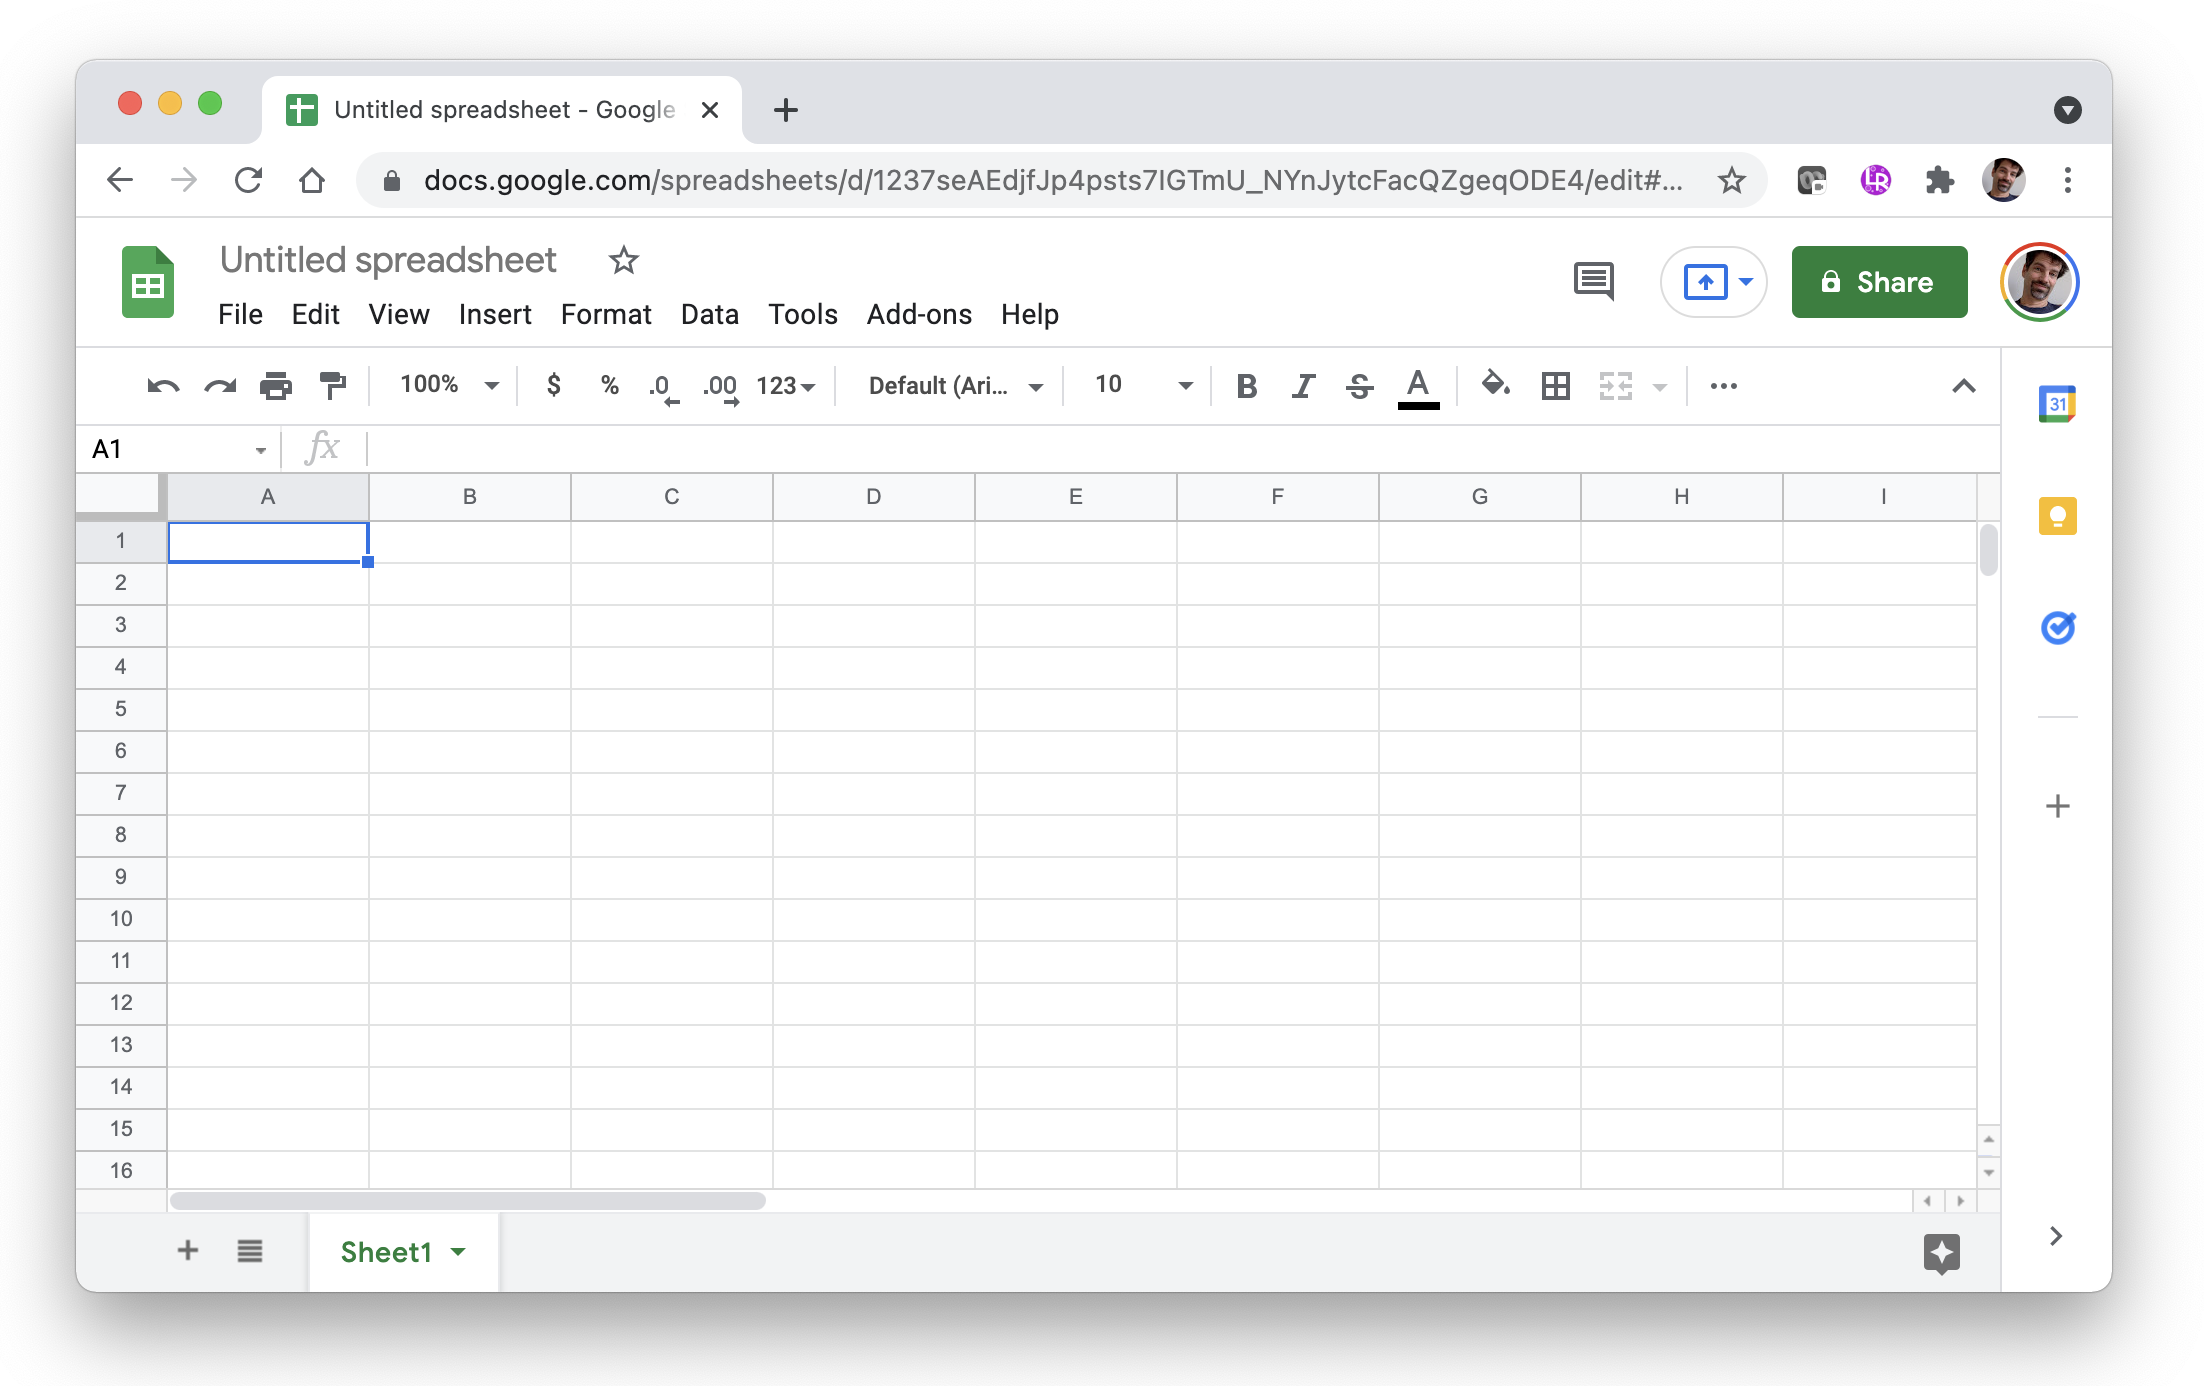
\includegraphics[width=0.6\textwidth]{BlankSheet.png}

Let's put some labels in the column:
\begin{itemize}
\item Select the first cell (A1) and type ``A number''.
\item Select the cell below it (A2) and type ``Another number''.
\item Select the cell below that one (A3) and type ``Their product''.
\item In the next column, type the number 5 in B1 and 7 in B2.
\end{itemize}

It should look like this:

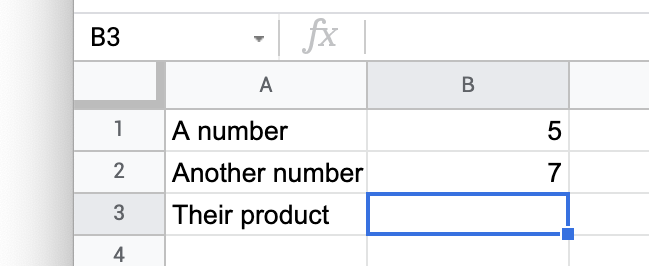
\includegraphics[width=0.5\textwidth]{NoFormulas.png}

Now put a formula in cell B3. Select B3, and type ``= B1 + B2''. The spreadsheet knows this is a formula because it starts with `=`. It will look like this as you type:\index{Spreadsheet!Entering formula}

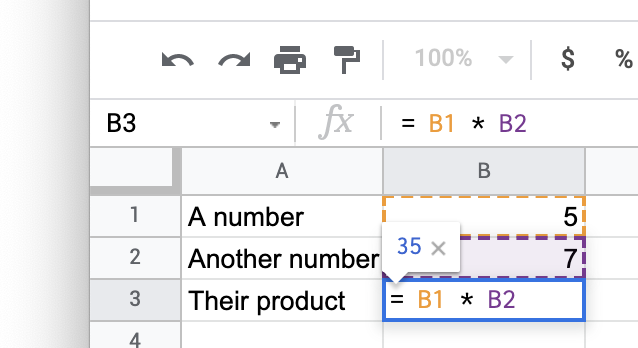
\includegraphics[width=0.5\textwidth]{TypingFirstFormula.png}

When you press Return or Tab, the spreadsheet will remember the formula, but display its value:

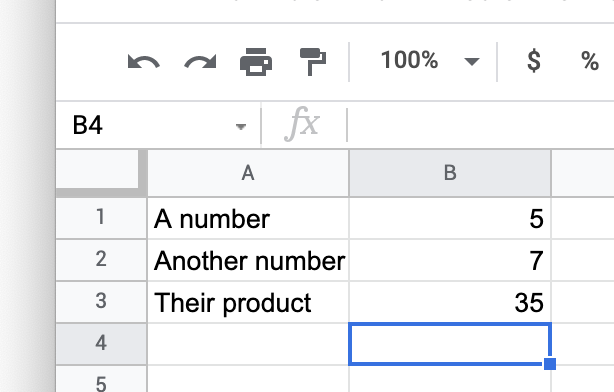
\includegraphics[width=0.5\textwidth]{FirstCalc.png}

If you change the values of cell B1 or B2, the cell B3 will automatically be recalculated. Try it.

\section{Formatting}

Every spreadsheet lets you change the formatting of your columns and cells. They are all a little different, so play with your spreadsheet a little now. Try to do the following:
\begin{itemize}
\item Set the background of the first column to light gray.
\item Right-justify the text in the first column.
\item Make the text in the first column bold.
\item Make the numbers in the second column have one digit after the decimal point.
\end{itemize}

It should look something like this:

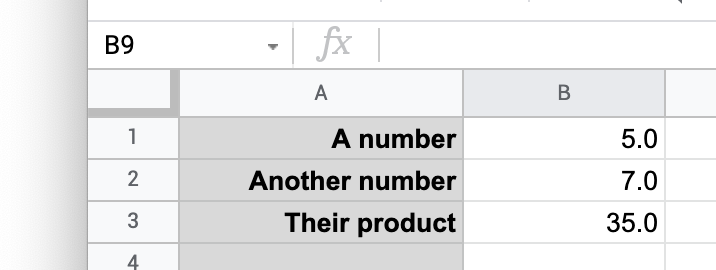
\includegraphics[width=0.6\textwidth]{FirstFormatting.png}

That's a spreadsheet. You have grid of cells. Each cell can hold a
value or a formula that uses values from other cells. The cells with
formulas automatically update as you edit the values in the other
cells.

\section{Comma-Separated Values}

A lot of data is exchanged in a file format called
\textit{Comma-Separated Values} or just CSV. Each CSV file holds one
table of data. It is a text file, and each line of text corresponds to
one row of data in the table. The data in each column is separated by
a comma. The first line of a CSV is usually the names of the
columns. A CSV might look like this:

\begin{Verbatim}
studentID,firstName,lastName,height,weight
1,Marvin,Sumner,260,45.3
2,Lucy,Harris,242,42.2
3,James,Boyd,261,44.2
\end{Verbatim}

In your digital resources for this module, you should have a file
called \path{1000cars.csv}. It is a CSV with only one column called
``speed''. The first few lines look like this:

\begin{Verbatim}
speed
33.8000
29.9920
34.8699
27.9936
\end{Verbatim}

There is a title line and 1000 data lines.

Import this CSV into your spreadsheet program. In Google Sheets, it looks like this:

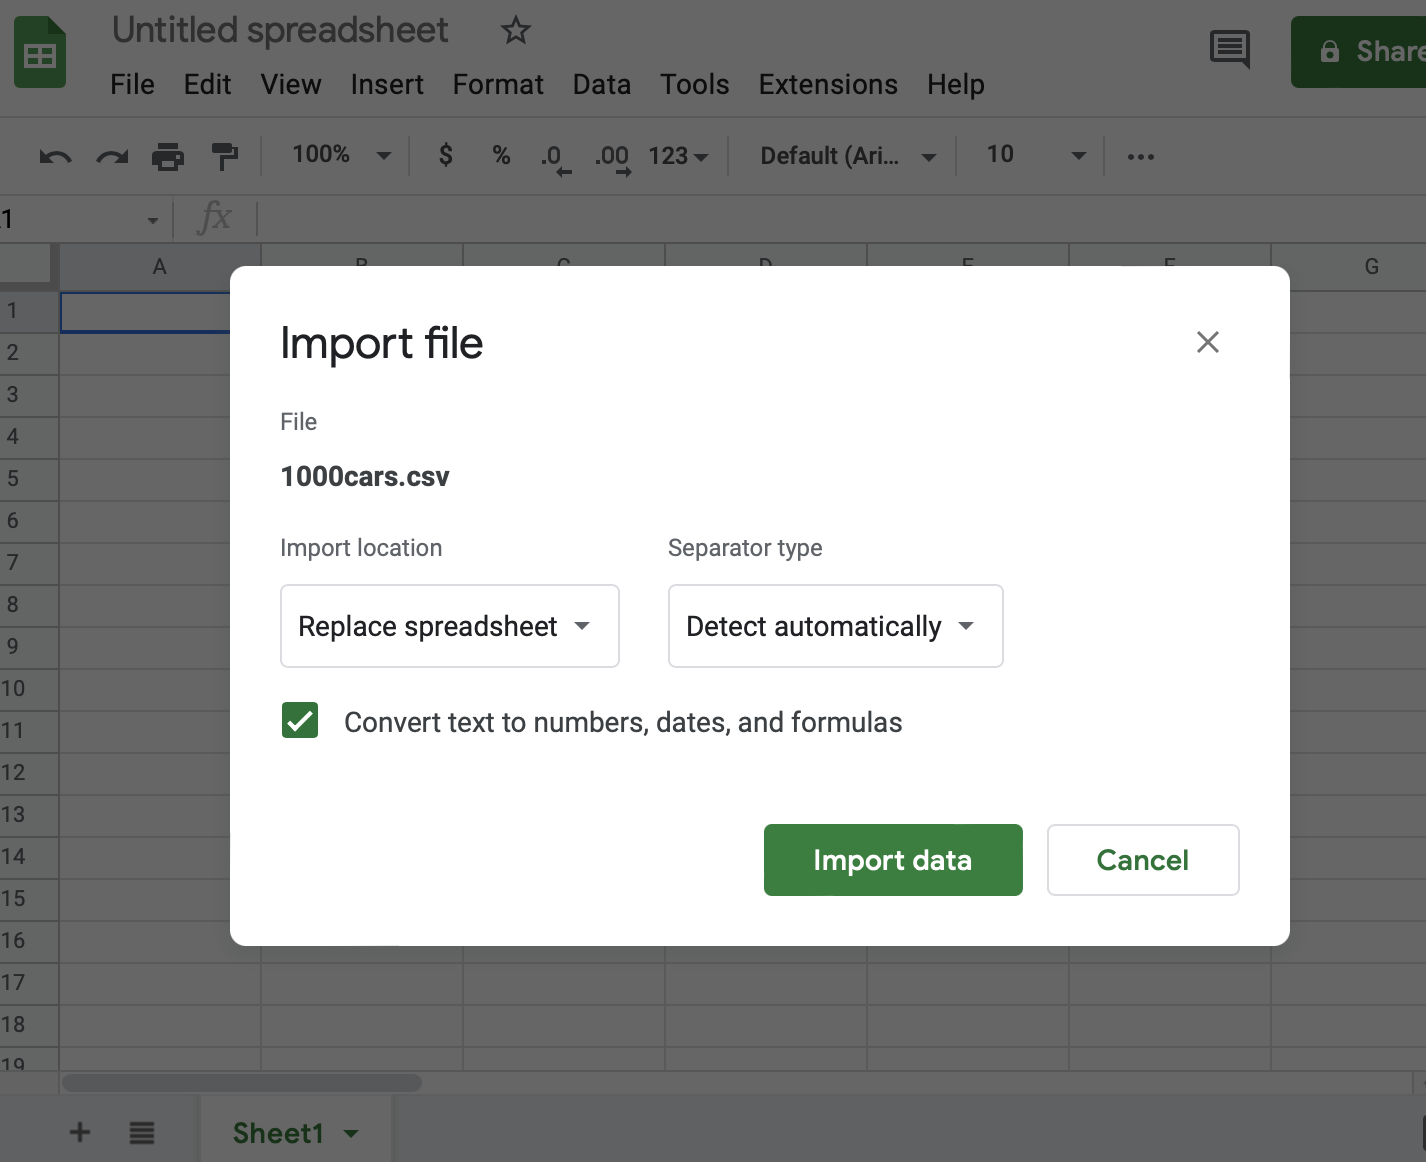
\includegraphics[width=0.5\textwidth]{ImportingCSV.png}

You should see a long, long column of data appear. (Mine goes from cell A2 through A1001.)

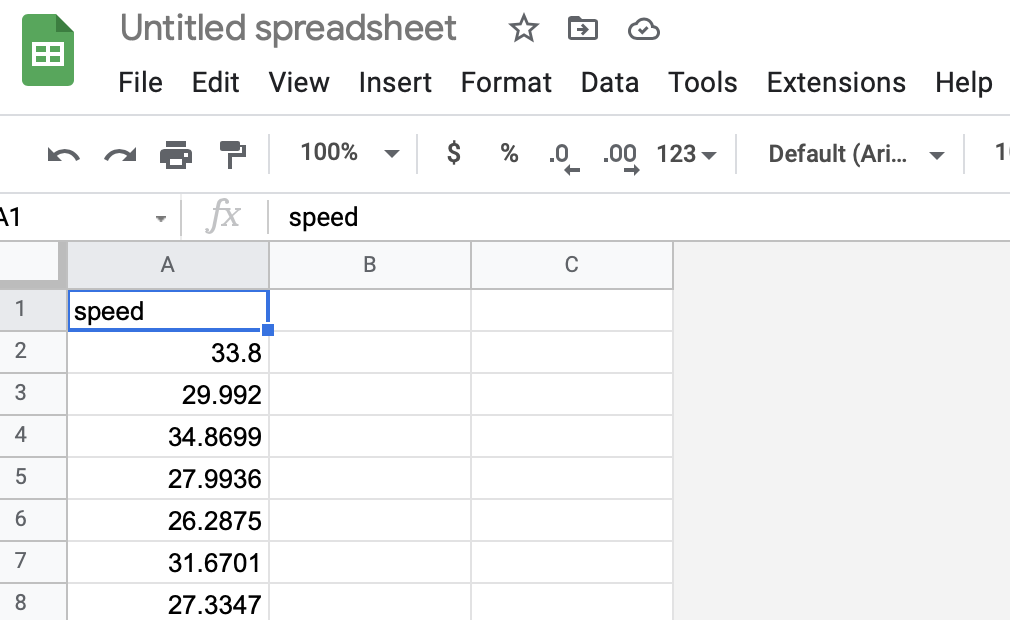
\includegraphics[width=0.5\textwidth]{ImportedCSV.png}

\section{Statistics in Spreadsheets}

Let's take the mean all 1000 numbers.  In cell B2, type in a label:
``Mean''. (Feel free to format your labels as you wish. Bolding is recommended.)

In cell C2, enter the formula ``=AVERAGE(A2:A1001)''. When
you press return, the cell will show the mean: 31.70441, if done correctly .

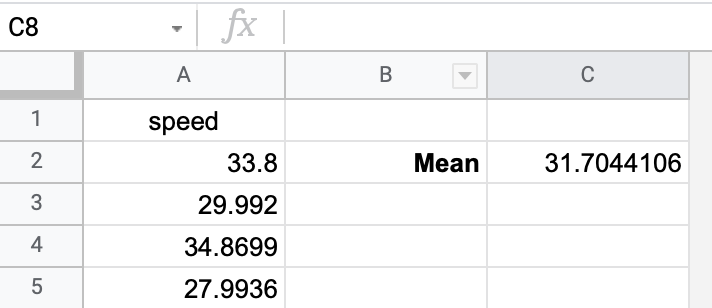
\includegraphics[width=0.4\textwidth]{Spread_mean.png}

Notice that by specifing that the function \pyfunction{AVERAGE} was to
be performed on a range of cells: cells A2 through A1001.

Do the calculations for variance, standard deviation, and median.

\begin{itemize}
\item The function for variance is \pyfunction{VAR}.
\item The function for standard deviation is \pyfunction{STDEV}.
\item The function for median is \pyfunction{MEDIAN}.
\end{itemize}

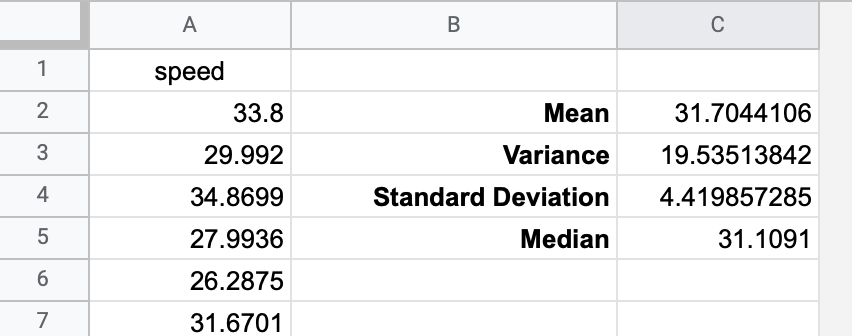
\includegraphics[width=0.4\textwidth]{var_stdev_median.png}

\section{Histogram}

Most spreadsheets have the ability to create a histogram. In Google
Sheets, you select the entire range A2:A1001 by selecting the first
cell and then shift-clicking the last. Then you choose
Insert$\rightarrow$Chart. In the inspector, change the type of the
chart to histogram. This will get you a basic histogram.
% Add: Define histogram or give example, defined in basic statistics, must come previous

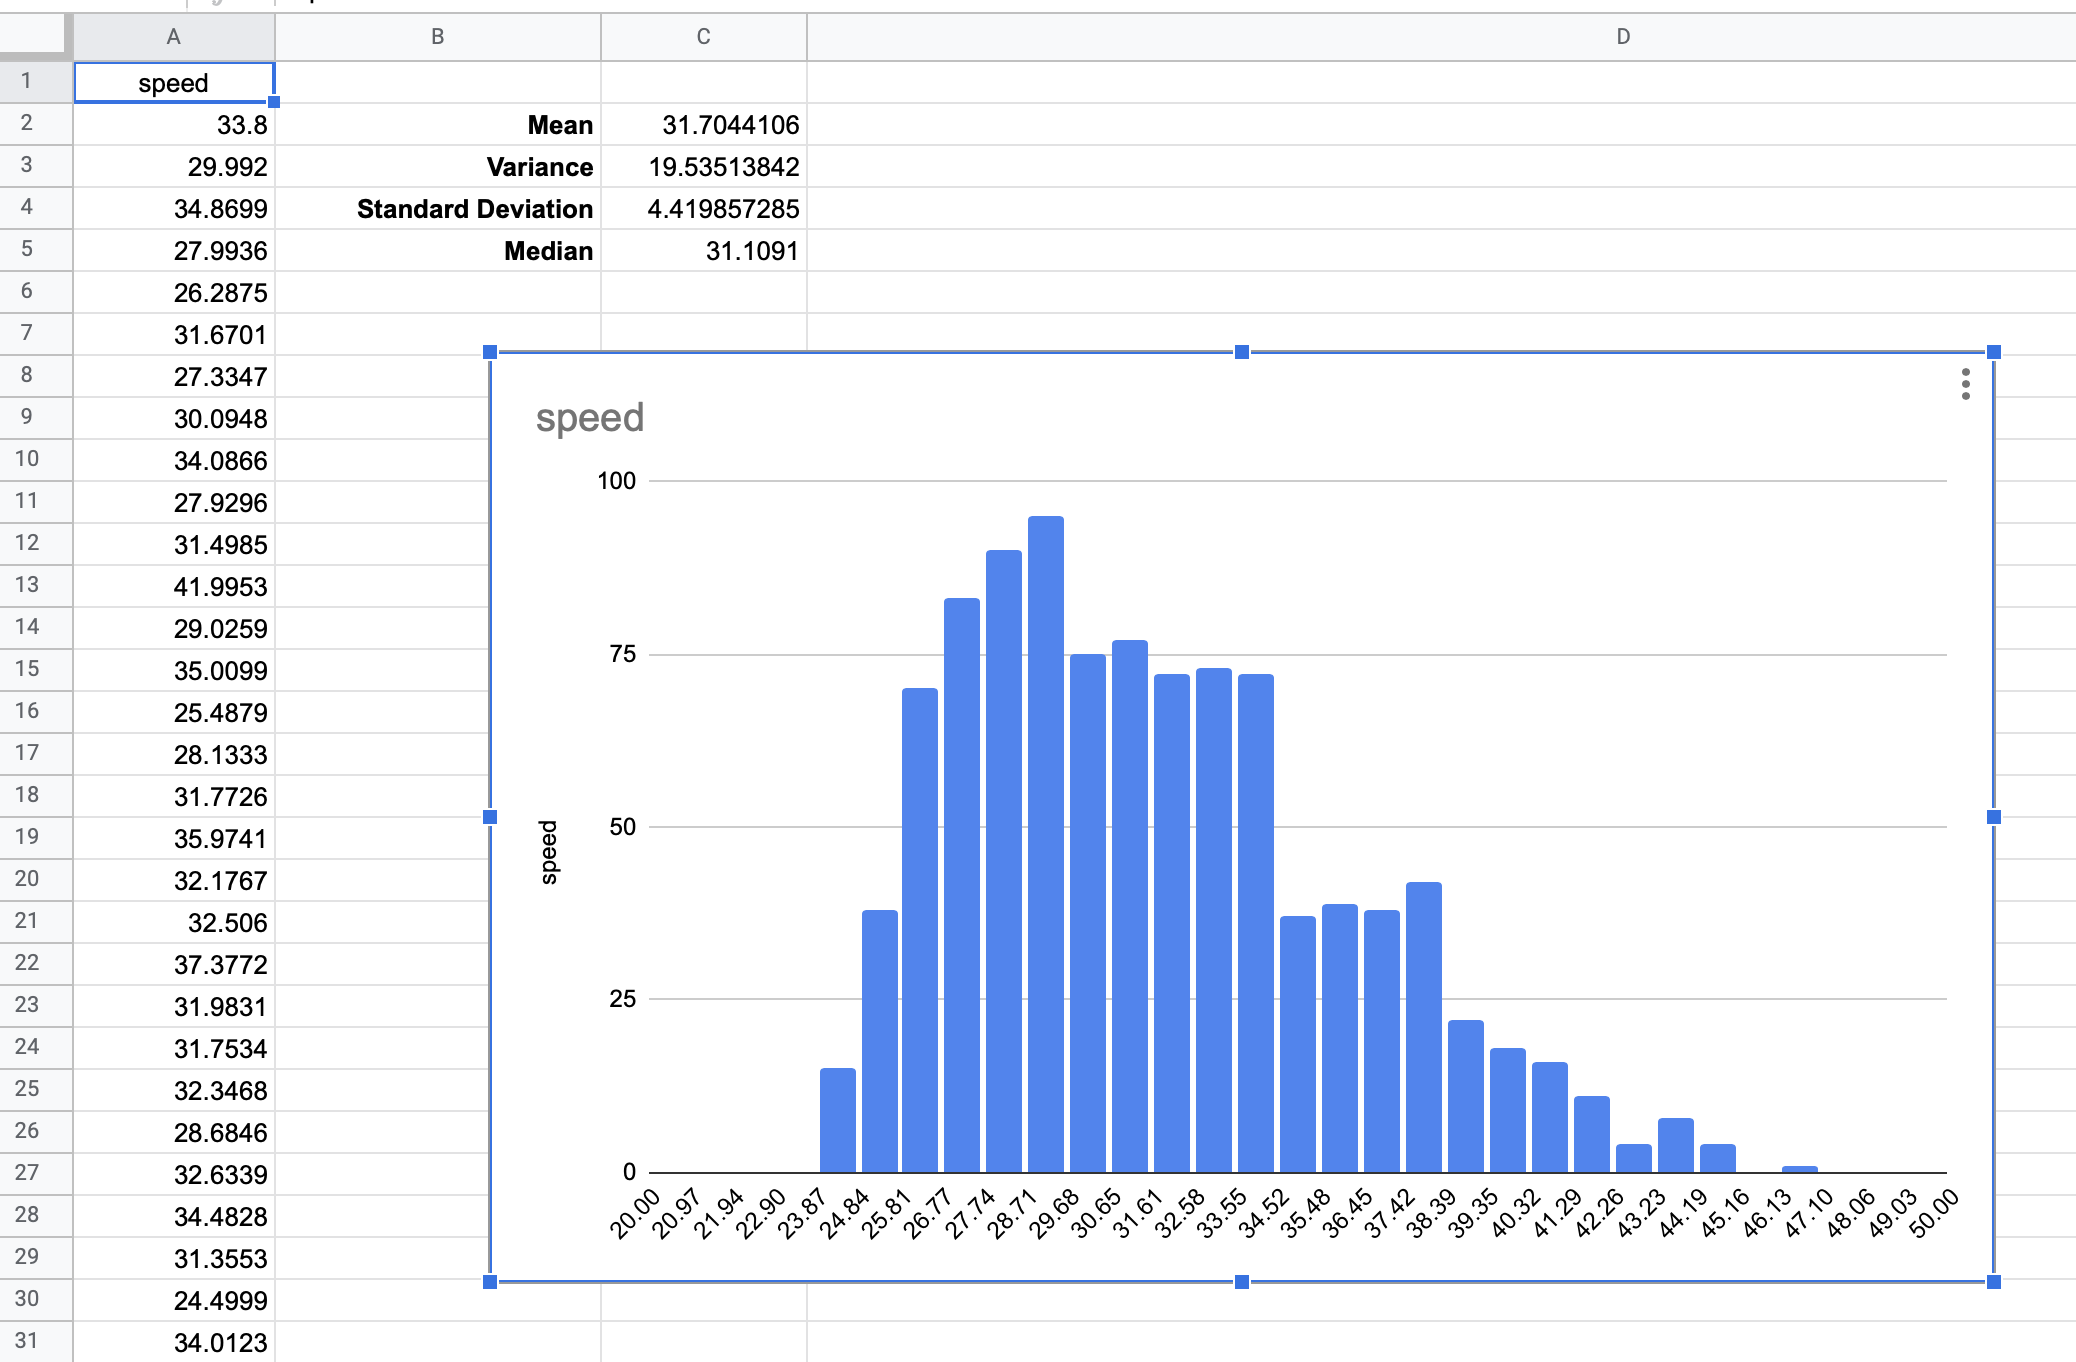
\includegraphics[width=0.7\textwidth]{default_histogram.png}

Play with the formatting to see how unquie you can make data. Here is an example:

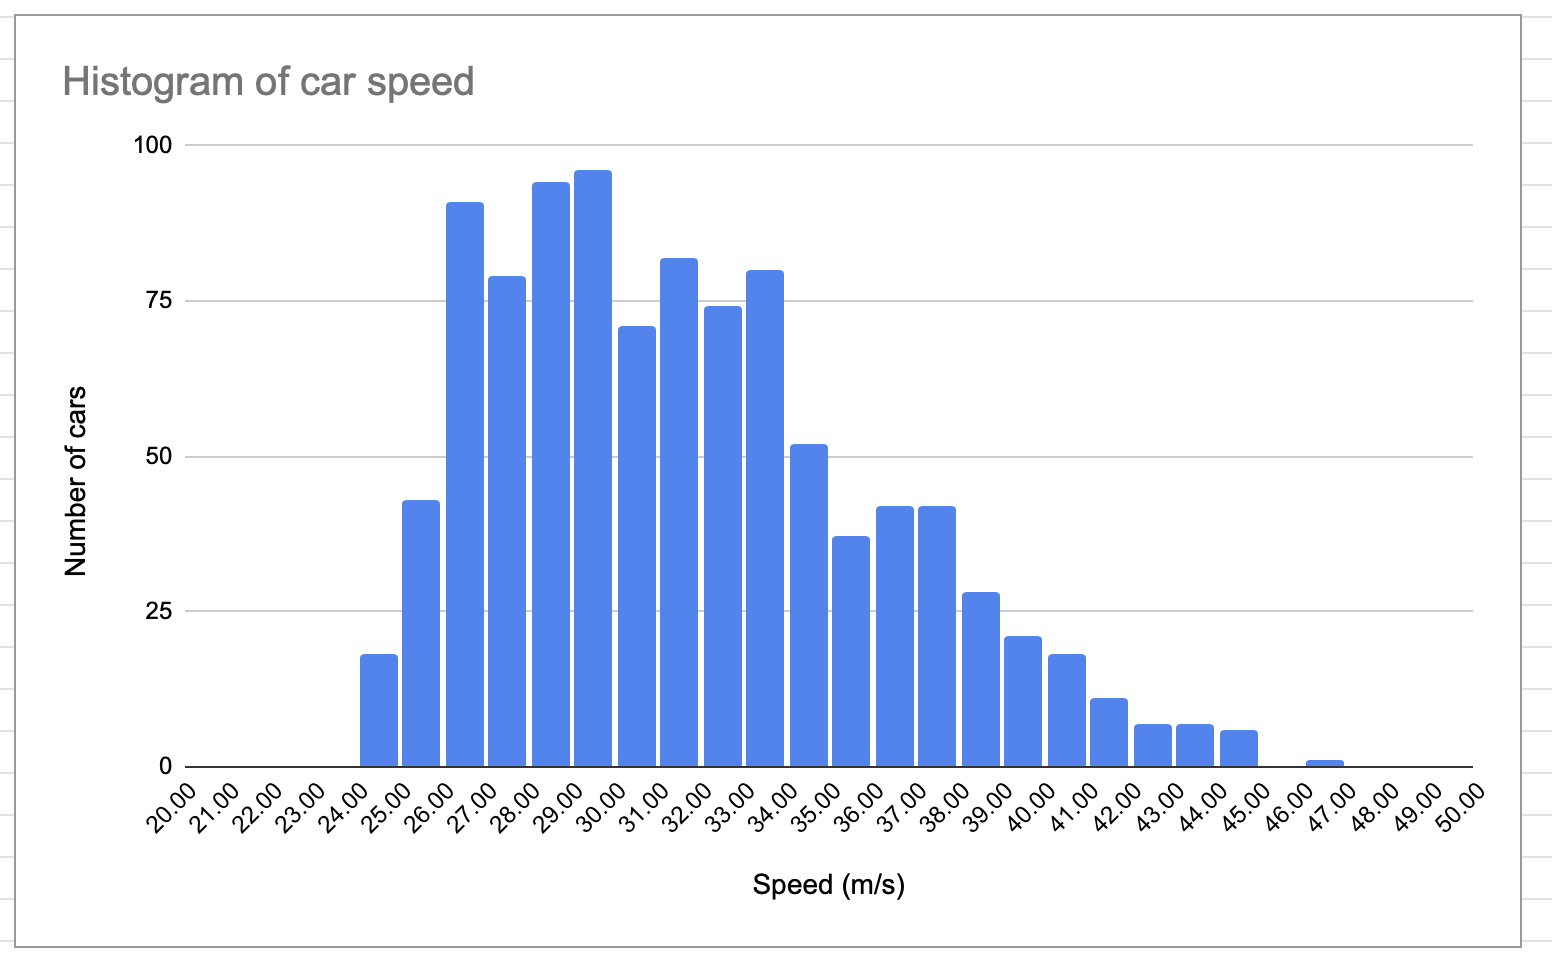
\includegraphics[width=0.8\textwidth]{final_histogram.png}

\begin{Exercise}[title={RMS}, label=rms_spreadsheet]

  In your spreadsheet, calculate the quadratic mean (the root-mean-squared) of the speeds.

  You will need the following three functions:
  \begin{itemize}
  \item \pyfunction{SUMSQ} returns the sum of the squares of a range of cells.
  \item \pyfunction{COUNT} returns the number of cells in a range that contain numbers.
  \item \pyfunction{SQRT} returns the square root of a number.
  \end{itemize}


\end{Exercise}
\begin{Answer}[ref=rms_spreadsheet]

The formula for the RMS is ``=SQRT(SUMSQ(A2:A1001)/COUNT(A2:A1001))''.
% KA: https://www.khanacademy.org/computing/ap-computer-science-principles/data-analysis-101/data-tools/a/learning-from-data-sets

\end{Answer}

\section{Cognitive Bias: The Dunning-Kruger Effect}

The less you know, the more confident you are.

When a person doesn't know all the nuance and context in which a question is
asked, the question seems simple. Thus the person tends to be confident in
their answer.  As they learn more about the complexity of the space in
which the question lives, they often realize the answer is not nearly so
obvious.

For example, a lot of people will confidently proclaim ``Taxes are too
high! We need to lower taxes.''  An economist who has studied
government budgets, deficits, history, and monetary policy, might say
something like ``Maybe taxes \emph{are} too high.  Or maybe they are
too low. Or maybe we are taxing the wrong things. It is a really
complex question.''

When I am talking with people about a particular topic, I do my best
to defer to the person in the conversation who I think has the most
knowledge in the area. If I disagree with the person, I try to figure
out why our opinions are different.

Similarly, you should assume that any opinion that is voiced in an
internet discussion is wildly over-simplified.  If you really care
about the subject, read a book by a respected expert. Yes, a whole
book -- there are few interesting topics that can be legitimately
explained in less than 100 pages.

\chapter{Introduction to Electricity}

What happens when you turn on a flashlight?  The battery in the
flashlight acts as an electron pump. The electrons flow through the
wires to the lightbulb (or LED).  As the electrons pass through the
lightbulb, they excite the molecules there, which give off light and
heat. (LEDs also give off light and heat, but they give off a lot less
heat.) Then the electrons return to the battery to be pumped around
again.

When electricity is flowing through a copper wire, the protons and
neutrons of the copper stay put while the electrons jump between the
atoms on their way from the battery to the lightbulb and back again.

\section{Units}

Electrons are very small, so to study them, scientists came up with a
unit that represents \textit{a lot} of electrons. 1 \textit{coulomb}
is about 6,241,509,074,460,762,608 electrons.  When 5 coulombs enter one end of the wire every second (and simultaneously 5 coulombs exit the other end), we say ``This wire is carrying 5 ampere of current.''\index{coulombs}

(Truthfully, we usually shorten ampere to just ``amp''.  This is
sometimes a little awkward because we often shorten the word
``amplifier'' to ``amp''. You should be able to tell which is which
from the context.)\index{amp or ampere}

If you look at the circuit breakers or fuses for your home's
electrical system, you'll see that each one is rated in amps.  For
example, maybe the circuit that supplies power to your kitchen has 10
amp circuit breaker. If for some reason, more than 10 amps tries to
pass through that wire, the circuit breaker will turn off the whole
circuit.

When it is on, your flashlight pushes something like 1 amp of current
through the lightbulb. (When it is off, there is no current in the
lightbulb.)

The lightbulb creates \textit{resistance} that the current pushes
through.\index{resistance} You can think of plumbing: The current is the amount of water
passing through a pipe. The resistence is something that tries to stop
the current -- like a ball of hair.  The battery is what creates the
pressure that pushes the current through the resistance. We call that
pressure \textit{voltage}.\index{voltage}

\section{Circuit Diagrams}

Here is a circuit diagram of your flashlight:

\begin{circuitikz}
\draw (0,0) to[battery1,invert,l=$3V$] ++(0,3)
to [switch,i=1A] ++(3,0)
to [lamp=$1\Omega$,bipoles/length=0.9cm] ++(0,-3) -- (0,0);
\end{circuitikz}

The lines are wires.  The symbols that we  will use:

\begin{tabular}{c c c c}
  Battery & Switch & Lamp & Resistor \\
\begin{circuitikz}
\draw (0,0) to[battery1] (2,0); 
\end{circuitikz}
&
\begin{circuitikz}
\draw (0,0) to[lamp,bipoles/length=0.9cm,l=$3 \Omega$] (2,0); 
\end{circuitikz}
&
\begin{circuitikz}
\draw (0,0) to[switch,/tikz/circuitikz/bipoles/length=1.0cm] (2,0); 
\end{circuitikz}
&
\begin{circuitikz}
\draw (0,0) to[R,  l=$3 \Omega$] (2,0); 
\end{circuitikz} \\
\end{tabular}

The battery pushes the electrons from one end and pulls them back in at the other,  so the circuit must go around in a circle for current to flow.  This is why the current stops flowing when the switch breaks the circuit.

You can think of a switch as having zero resistance when it is closed and infinite resistance when it is open.

For our purposes, a lamp is just a resistor that gives off light.

\section{Ohm's Law}

Resistance is measured in \textit{ohms}, and we use a Greek capital omega for that: $\Omega$  

Voltage is measured in
\textit{volts}.\index{ohms}\index{volts}

\begin{mdframed}[style=important, frametitle={Ohm's Law}]\index{Ohm's law}
  Whenever a voltage $V$ is pushing a current $I$ through a resistance of $I$, the following is true:

  $$V = IR$$

  where $V$ is in volts, $I$ is in amps, and $R$ is in ohms.
\end{mdframed}

\section{Power and Watts}

\begin{mdframed}[style=important, frametitle={Joule's Law}]\index{Joule's law}

  When a current $I$ is passing through a resistance $R$, the power consumed is
  
  $$W = I^2 R$$

  where $W$ is in watts, $I$ is in amps, and $R$ is in ohms.
\end{mdframed}

Of course $V = IR$, so we can extend this to:

$$W = I^2 R = I V = \frac{V^2}{R}$$

Your flashlight's batteries probably provide about 3 volts.  How much
battery power is the flashlight using when it is on? The power (in
watts) produced by the battery is the product of the voltage (in
volts) and the current (in amps). So your flashlight giving off $3
volts \times 1 amp = 3 watts$ of power. Some of that power is given
off as light, some as heat.\index{watts}

A watt is 1 joule of energy per second. We say that a watt is a
measure of \textit{power}.

When we talk about how much energy is stored in a battery, we use a
unit like kilowatt-hour.  A kilowatt-hour is equivalent to 3.6 million
joules.

\section{Another great use of RMS}

In many electrical problems, the voltage fluctuates a lot.  For
example, the fluctuations in voltage make the sound come out of an
audio speaker.

You can use the root-mean-squared of the voltage to figure out the average power
your speaker is consuming.

Lets say that the RMS of the voltage you are sending to the speaker is $V_{rms}$
and the resistance of the speaker is $R$ ohms, then the power consumed
by the speaker is:

$$P = \frac{V_{rms}^2}{R}$$

Similarly, if you know the RMS of the current you are pushing through
the speaker is $I_{rms}$, then the power consumed by the speaker is:

$$P = I_{rms} R$$


\chapter{DC Circuit Analysis}

In the most basic circuit, you have only a battery and a resistor:

\begin{circuitikz}
\draw (0,0) to[battery1,invert,l=$6V$] ++(0,3)
to ++(3,0)
to [R=$3\Omega$, /tikz/circuitikz/bipoles/length=1.0cm,i=2A] ++(0,-3) -- (0,0);
\end{circuitikz}

In this case, you only need Ohm's Law: $V = I R$.  In this case, $6V = 3\Omega \times 2A$.
% ADD: Define Ohm's Law
\begin{Exercise}[title={Ohm's Law}, label=ohms_check]

  How many amps are going around the circuit?
  
  \vspace{1cm}

\begin{circuitikz}
\draw (0,0) to[battery1,invert,l=$24V$] ++(0,3)
to ++(3,0)
to [R=$6\Omega$, /tikz/circuitikz/bipoles/length=1.0cm,i={? A}] ++(0,-3) -- (0,0);
\end{circuitikz}

  
\end{Exercise}
\begin{Answer}[ref=ohms_check]

  $V = I R$ so $I = \frac{V}{R} = \frac{24V}{6\Omega} = 4A$.
  
\end{Answer}
% KA: https://youtu.be/F_vLWkkOETI

\section{Resistors in Series}

When you have two resistors wired together in a long line, we say they
are ``in series''.  If you have two resistors $R_1$ and $R_2$ wired in
series, the total resistance is $R_1 + R_2$.

In this diagram, for example, the total resistance is $5\Omega$.

\begin{circuitikz}
\draw (0,0) to[battery1,invert,l=$10V$] ++(0,5)
to ++(3,0)
to [R=$3\Omega$] ++(0,-2.5)
to [R=$2\Omega$] ++(0,-2.5) -- (0,0);
\end{circuitikz}

The current flowing through the circuit, then, is $10/4 = 2A$.

By Ohm's law, the voltage drop across the upper resistor is $I R = 2A \times 3\Omega = 6V$.

The voltage drop across the lower resistor is $I R = 2A \times 2\Omega = 4V$.

Notice that the battery pumps the voltage up to $10V$, then the two
resistors drop it by exactly $10V$. This is known as ``Kirchhoff's
Voltage Law'':
% KA: https://youtu.be/4rsswT_Rv1M

\begin{mdframed}[style=important, frametitle={Kirchhoff's Voltage Law}]\index{Kirchhoff's voltage law}
As you make a loop around a circuit, the sum of the voltage increase
must equal the sum of the voltage decrease.
\end{mdframed}

The negative end of the battery as connected to ``ground'' (
it has zero voltage), then we can draw a diagram with the
voltages(That symbol in the lower right represents a connection to ground).

\begin{circuitikz}
\draw (0,0) to[battery1,invert,l=$6V$] ++(0,5) 
to [-*] ++(3,0) node[anchor=west] {10V}
to [R=$3\Omega$,-*] ++(0,-2.5) node[anchor=west] {4V}
to [R=$2\Omega$,-*] ++(0,-2.5) node[anchor=west]{0V} node[ground]{} --(0,0);
\end{circuitikz}


\begin{Exercise}[title={Resistors In Series}, label=series_resistor]

  What is the current going around the circuit?
  
  What is the voltage drop across each resistor?
  
  \vspace{1cm}
\begin{circuitikz}
\draw (0,0) to[battery1,invert,l=$16V$] ++(0,5) 
to [-*] ++(3,0) node[anchor=west] {16V}
to [R=$5\Omega$,-*] ++(0,-2.5) node[anchor=west] {?}
to [R=$3\Omega$,-*] ++(0,-2.5) node[anchor=west]{0V} node[ground]{} --(0,0);
\end{circuitikz}


\end{Exercise}
\begin{Answer}[ref=series_resistors]

  There is a total resistance of $8\Omega$, so your 16V will push 2A
  of current around the circuit.

  2A going through a $5\Omega$ resistor represents a 10V drop.

  2A going through a $3\Omega$ resitor represents a 6V drop.
  
\end{Answer}


\section{Resistors in Parallel}

Look at this circuit. Note that the current can go two different paths.

\begin{circuitikz}
\draw (0,0) to[battery1,invert,l=$12V$] ++(0,3)
to ++(3,0)
to [R=$2\Omega$, /tikz/circuitikz/bipoles/length=1.0cm] ++(0,-3) -- (0,0);
\draw (3,3) -- (5,3)
to [R=$3\Omega$, /tikz/circuitikz/bipoles/length=1.0cm] ++(0,-3) -- (3,0);
\end{circuitikz}

There is 12 volts pushing current through both resistors. So 6A will
go through the 2$\Omega$ resistor and 4A will go through the 3$\Omega$
resistor.

\begin{circuitikz}
\draw (0,0) to[battery1,invert,l=$12V$] ++(0,3)
to ++(3,0)
to [R=$2\Omega$, /tikz/circuitikz/bipoles/length=1.0cm,i=6A] ++(0,-3) -- (0,0);
\draw (3,3) -- (5,3)
to [R=$3\Omega$, /tikz/circuitikz/bipoles/length=1.0cm,i=4A] ++(0,-3) -- (3,0);
\end{circuitikz}

Thus, a total of 10 A will be going through the battery.

Imagine you are a battery. You can't see that you have two resistors.
What does it feel like to you? $\frac{V}{I} = R$, and $V= 12$ and $I =
10$.  So the effective resistance of the two resistors in parallel is
$\frac{12}{10}$ or $\frac{6}{5} \Omega$.

\begin{mdframed}[style=important, frametitle={Resistance in Parallel}]\index{resistance!in parallel}
If you have several resistances $R_1, R_2, \ldots, R_n$ wired in
parallel, their effective resistance $R_t$ is given by

$$\frac{1}{R_t} = \frac{1}{R_1} + \frac{1}{R_2} + \ldots + \frac{1}{R_n}$$

\end{mdframed}

In our example:

$$\frac{1}{R_t} = \frac{1}{2} + \frac{1}{3} = \frac{5}{6}$$

Thus $R_t =  \frac{6}{5}\Omega$.

\begin{Exercise}[title={Resistors In Parallel}, label=parallel_resistors]

  What is the current going through the battery?
  What is the drop over the $4\Omega$ resistor?
  What is the current in each branch?

  \vspace{1cm}

  \begin{circuitikz}
\draw (0,0) to[battery1,invert,l=$12V$] ++(0,3)
to [R=$4\Omega$, /tikz/circuitikz/bipoles/length=1.0cm] ++(3,0) node [yshift=0.3cm] {? V}
to [R=$6\Omega$, /tikz/circuitikz/bipoles/length=1.0cm,i={? A}] ++(0,-3) node[ground]{} -- (0,0);
\draw (3,3) -- (5,3)
to [R=$3\Omega$, /tikz/circuitikz/bipoles/length=1.0cm,i={? A}] ++(0,-3) -- (3,0);
\end{circuitikz}

\end{Exercise}
\begin{Answer}[ref=parallel_resistors]
  The effective resistance of the $6\Omega$ and the $3\Omega$ is $2\Omega$ because 

  $$\frac{1}{R_T} = \frac{1}{6} + \frac{1}{3} == \frac{1}{2}$$

  So the battery experiences a resistance of $4\Omega + 2\Omega =
  6\Omega$.  A $12V$ will push 2A through a resistance of $6\Omega$.

  The voltage drop across the $4\Omega$ resistor is $2A \times 4\Omega
  = 8V$. Thus there will be a 4V drop across the two resistors in
  parallel.  So 2/3 A will flow through the $6\Omega$ resistor. 4/3 A
  will flow through the $3\Omega$ resistor.

    \begin{circuitikz}
\draw (0,0) to[battery1,invert,l=$12V$] ++(0,3)
to [R=$4\Omega$, /tikz/circuitikz/bipoles/length=1.0cm] ++(3,0) node [yshift=0.3cm] {8 V}
to [R=$6\Omega$, /tikz/circuitikz/bipoles/length=1.0cm,i={2/3 A}] ++(0,-3) node[ground]{}-- (0,0);
\draw (3,3) -- (5,3)
to [R=$3\Omega$, /tikz/circuitikz/bipoles/length=1.0cm,i={4/3 A}] ++(0,-3) -- (3,0);
\end{circuitikz}

% Image: https://circuitdigest.com/sites/default/files/inlineimages/u/DC-Circuit-Theory_0.png
  
\end{Answer}

\section{Cognitive bias: Survivorship bias}

You will pay more attention to those that survived a process than
those who failed.

After looking at a lot of old houses, you might say ``In the 1880s,
they built great houses.'' However, you haven't seen the houses that
were built in the 1880s and didn't survive.  Which houses tended to
survive for a long time? Only the great houses -- you are
basing your opinion on a very skewed sample.


\chapter{Charge}

If you rub a balloon against your hair, it will stick to a wall. We
say that it has gotten an \textit{electrical charge}. It stole some
electrons from your hair, and now the ballon has slightly more
electrons than protons.  We say that it has a negative electrical
charge.

Objects with slight more protons than electrons have a positive charge.

The charge is measured in coulombs. The charge of a single proton is
about $1.6 \times 10^{-19}$ coulombs.

An object with a negative charge and an object with a positive charge
will be attracted to each other. Two objects with the same charge will
be repelled by each other.

\begin{mdframed}[style=important, frametitle={Coulomb's Law}]\index{Coulomb's law}

  If two objects with charge $q_1$ and $q_2$ (in coulombs) are $r$ meters from each other, the force of attraction or repulsion is given by

  $$F = K\frac{\lvert q_1 q_2 \rvert}{r^2}$$

    where $F$ is in newtons and $K$ is Coulomb's constant: about $8.988 \times 10^9$.
  
\end{mdframed}


\begin{Exercise}[title={Coulomb's Law}, label=charged_balloons]

Two balloons are charged with an identical quantity and type of
charge: $-5 \times 10^{-9}$ coulombs. They are held apart at a
separation distance of 12 cm. Determine the magnitude of the
electrical force of repulsion between them. 
  
\end{Exercise}
\begin{Answer}[ref=charged_balloons]

  $$F = K\frac{\lvert q_1 q_2 \rvert}{r^2} = (8.988 \times 10^9) \frac{(-5 \times 10^{-9})(-5 \times 10^{-9})}{0.12^2} = \frac{224.7 \times 10^{-9}}{0.0144} = 15.6 \times 10^{-6}$$

  15.6 micronewtons.
  
\end{Answer}

\section{Lightning}

A cloud is a cluster of water droplets and ice particles. These
droplets and ice particles are always moving up and down through the
cloud. In this process, electrons get stripped off and end up on the
water droplets at the bottom of the cloud. The air between the
droplets is a pretty good insulator, and the electrons are reluctant
to jump anywhere. However, eventually the charge gets so strong that
even the insulating properties of the air is not enought to prevent
the jump.

A lot of lightning moves within a cloud or between clouds. However, a
few jump to the earth. These bolts of lightning vary in the amount of
electrons they carry, but the average is about 15 coulombs.

The electrons heat the air they pass through. The air expands
suddenly, and the resulting shockwave is thunder.

\section{But...}

This idea that opposite charges attract creates some heavy questions
that you do not yet have the tools to work with. So the answer is
basically ``Don't ask that question now!''

However, you probably have these questions, so I will wave my hands in
the direction of the answers.

The first is ``In any atom bigger than hydrogen, there are multiple
protons in the nucleus. Why don't the protons push each other out of
the nucleus?''

We aren't ready talk about it, but there is a force called \textit{the
  nuclear force} which pulls the protons and neutrons in the nucleus
of the atom together.

Another question is ``Why do the electrons whiz around in a cloud so
far from the nucleus of the atom? Negatively charged electrons should
cling to the protons in the center, right?''

We aren't ready to talk about it, but quantum mechanics tells us that
electrons like to live a certain specific energy levels. Cuddling with
a proton isn't one of those levels.

\graphicspath{{../../Modules/TrianglesCircles/}}
\chapter{Angles}

In the videos I'm about to recommend, the narrator will talk about
lines, line segments, and rays. When mathematicians talk about
\emph{lines}, they mean a straight line that goes forever in both
directions. Pick any two points on a line; the points between them are
a \emph{line segment}. If you take any line, pick a point on that line
and discard all the points on one side of the point, that is a
\emph{ray}. All three are infinitely thin.

\begin{tikzpicture}[scale=1.5]
  \coordinate (a) at (-0.3, -0.6);
  \coordinate (d) at (1.3, 2.6);
  \draw [<->](a)--node [right]{"Line"}(d);
\end{tikzpicture}
\hspace{10mm}
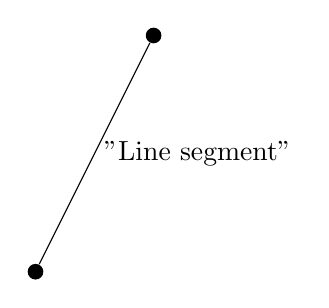
\begin{tikzpicture}[scale=1.5]
  \coordinate [circle, fill, inner sep=2pt] (b) at (0,0) ;
  \coordinate [circle, fill, inner sep=2pt] (c) at (1, 2) ;
  \draw (b)--node [right]{"Line segment"}(c);
\end{tikzpicture}
\hspace{6mm}
\begin{tikzpicture}[scale=1.5]
  \coordinate [circle, fill, inner sep=2pt] (b) at (0,0) ;
  \coordinate (d) at (1.3, 2.6);
  \coordinate (lab) at (0.8, 1.0);
  \draw [->](b)--node[right] {"Ray"} (d)  ;
\end{tikzpicture}


Watch the following videos from Khan Academy:
\begin{itemize}
\item Introduction to angles: \url{https://youtu.be/H-de6Tkxej8}
\item Measuring angles in degrees: \url{https://youtu.be/92aLiyeQj0w} 
\end{itemize}

When two lines cross, they form four angles:

\begin{tikzpicture}[scale=3]
  \coordinate (a) at (0, 1.5);
  \coordinate (b) at (1.6, 2);
  \coordinate (c) at (1.6, 1.5);
  \coordinate (d) at (0, 1);
  \coordinate [circle, fill, inner sep=2pt](e) at (0.8, 1.5) ;
  \draw [->](e)--(a) node[left] {$A$}  ;
  \draw [->](e)--(b) node[right] {$B$}  ;
  \draw [->](e)--(c) node[right] {$C$}  ;
  \draw [->](e)node[above]{$E$}--(d) node[left] {D} ;
  \pic [draw, <->, "$\scriptstyle  \angle AEB$ ", angle radius = 0.8cm, angle eccentricity=1.3] {angle = b--e--a};
  \pic [draw, <->, "$\scriptstyle  \angle BEC$ ", angle radius = 1.1cm, angle eccentricity = 1.5] {angle = c--e--b};
  \pic [draw, <->, "$\scriptstyle  \angle CED$ ", angle radius = 0.8cm, angle eccentricity=1.3] {angle = d--e--c};
  \pic [draw, <->, "$\scriptstyle  \angle DEA$ ", angle radius = 1.1cm, angle eccentricity=1.5] {angle = a--e--d};
\end{tikzpicture}

What do we know about those angles?
\begin{itemize}
\item The sum of any two adjacent angles add to be $180^{\circ}$.  So, for example, $m \angle AEB + m \angle BEC = 180^\circ$.
\item The sum of all four angles is $360^\circ$.
\item Angles opposite each other are equal. So, for example, $m \angle AEB = m \angle CED$.
\end{itemize}

When two lines are perpendicular, the angle between them is $90^\circ$ and we say they meet at a \emph{right angle}. There is a notation for this:

\begin{tikzpicture}[scale=1.5]
  \coordinate (a) at (0, 1.5);
  \coordinate (b) at (0, 0);
  \coordinate (c) at (1.5, 0);
  \draw [->](b)--(a)  ;
  \draw [->](b)--(c)  ;
  \draw (b) rectangle ++(0.2,0.2) ;
\end{tikzpicture}
 
When an angle is less than $90^\circ$, it is said to be
\emph{acute}. When an angle is more than $90^\circ$, it is said to be
\emph{obtuse}.

\begin{tikzpicture}[scale=3]
  \coordinate (a) at (0.4, 0.6);
  \coordinate (b) at (0, 0);
  \coordinate (c) at (0.9, 0);
  \draw [->](b)--(a)  ;
  \draw [->](b)--(c)  ;
  \pic [draw, <->, "acute", angle radius = 1cm, angle eccentricity=1.5] {angle = c--b--a};
  \end{tikzpicture}
\hspace{2cm}
\begin{tikzpicture}[scale=3]
  \coordinate (a) at (1, 0.6);
  \coordinate (b) at (0.5, 0);
  \coordinate (c) at (0, 0);
  \draw [->](b)--(a)  ;
  \draw [->](b)--(c)  ;
  \pic [draw, <->, "obtuse", angle radius = 0.6cm, angle eccentricity=1.5] {angle = a--b--c};
  \end{tikzpicture}

\chapter{Introduction to Triangles}

Connecting any three points with three line segments will get you a
triangle. Here is the triangle $ABC$ created by connecting three points $A$, $B$, and $C$:\index{triangle}

\begin{tikzpicture}[scale=1.5]
  \coordinate [circle, fill, inner sep=2pt] (a) at (0,0) ;
  \coordinate [circle, fill, inner sep=2pt] (b) at (1, 2) ;
  \coordinate [circle, fill, inner sep=2pt] (c) at (3,0) ;
  \draw (a)--(b) node [outer sep=3pt, above]{$B$};
  \draw (b)--(c) node[outer sep=3pt, right]{$C$};
  \draw (c)--(a) node[outer sep=3pt, left]{$A$};
\end{tikzpicture}

\section{Equilateral and Isosceles Triangles}

We talk a lot about the length of the sides of triangles. If all three sides of the triangle are the same length, we say it is an \emph{equilateral triangle}:\index{equilateral triangle}

\begin{tikzpicture}[scale=1.5]
  \coordinate [circle, fill, inner sep=2pt] (a) at (0,0) ;
  \coordinate [circle, fill, inner sep=2pt] (b) at (1.5, 2.6) ;
  \coordinate [circle, fill, inner sep=2pt] (c) at (3,0) ;
  \draw (a)--(b) node [outer sep=3pt, above]{$B$};
  \draw (b)--(c) node[outer sep=3pt, right]{$C$};
  \draw (c)--(a) node[outer sep=3pt, left]{$A$};
  \tkzMarkSegment[pos=.5,mark=||](a,b)
  \tkzMarkSegment[pos=.5,mark=||](b,c)
  \tkzMarkSegment[pos=.5,mark=||](c,a)
\end{tikzpicture}

If only two sides of the triangle are the same length, we say it is an \emph{isosceles triangle}:\index{isoscelese triangle}

\begin{tikzpicture}[scale=1.3]
  \coordinate [circle, fill, inner sep=2pt] (a) at (0,0) ;
  \coordinate [circle, fill, inner sep=2pt] (b) at (1.5, 4) ;
  \coordinate [circle, fill, inner sep=2pt] (c) at (3,0) ;
  \draw (a)--(b) node [outer sep=3pt, above]{$B$};
  \draw (b)--(c) node[outer sep=3pt, right]{$C$};
  \draw (c)--(a) node[outer sep=3pt, left]{$A$};
  \tkzMarkSegment[pos=.5,mark=||](a,b)
  \tkzMarkSegment[pos=.5,mark=||](c,b)
\end{tikzpicture}

The shortest distance between two points is always the straight line
between them. Thus, you can be certain that the length of one side
will \emph{always} be less than the sum of the lengths of the
remaining two sides. This is known as the \emph{triangle inequality}.\index{triangle inequality}

For example, in this diagram $c$ must be less than $a + b$.

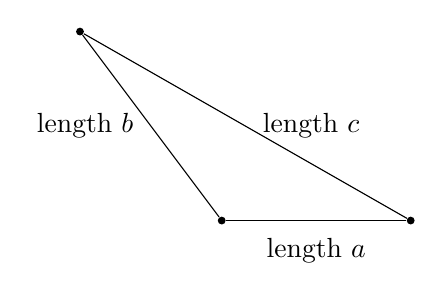
\begin{tikzpicture}[scale=1.2]
  \coordinate [circle, fill, inner sep=1pt] (a) at (1.5,0) ;
  \coordinate [circle, fill, inner sep=1pt] (b) at (0,2) ;
  \coordinate [circle, fill, inner sep=1pt] (c) at (3.5,0) ;
  \draw (a)--node[outer sep=3pt, left]{length $b$}(b) ;
  \draw (b)--node[outer sep=3pt, right]{length $c$}(c) ;
  \draw (c)--node[outer sep=3pt, below]{length $a$}(a) ;
\end{tikzpicture}

\section{Interior Angles of a Triangle}

We also talk a lot about the interior angles of a triangle:

\begin{tikzpicture}[scale=2]
  \coordinate [circle, fill, inner sep=2pt] (a) at (0,0) ;
  \coordinate [circle, fill, inner sep=2pt] (b) at (1, 2) ;
  \coordinate [circle, fill, inner sep=2pt] (c) at (3,0) ;
  \draw (a)--(b) node [outer sep=3pt, above]{$B$};
  \draw (b)--(c) node[outer sep=3pt, right]{$C$};
  \draw (c)--(a) node[outer sep=3pt, left]{$A$};
  \pic [draw, <->, "$a$", angle eccentricity=1.5] {angle = c--a--b};
  \pic [draw, <->, "$b$", angle eccentricity=1.5] {angle = a--b--c};
  \pic [draw, <->, "$c$", angle eccentricity=1.5] {angle = b--c--a};
\end{tikzpicture}

A triangle where one of the interior angles is a right angle is said to be a \emph{right triangle}:\index{right triangle}

\begin{tikzpicture}[scale=1.2]
  \coordinate [circle, fill, inner sep=2pt] (a) at (0,0) ;
  \coordinate [circle, fill, inner sep=2pt] (b) at (0,4) ;
  \coordinate [circle, fill, inner sep=2pt] (c) at (3,0) ;
  \draw (a)--(b) node [outer sep=3pt, above]{$B$};
  \draw (b)--(c) node[outer sep=3pt, right]{$C$};
  \draw (c)--(a) node[outer sep=3pt, left]{$A$};
  \pic [draw,angle eccentricity=1.5] {right angle = c--a--b};
\end{tikzpicture}

If a triangle has an obtuse interior angle, it is said to be an \emph{obtuse triangle}:\index{obtuse triange}

\begin{tikzpicture}[scale=1.2]
  \coordinate [circle, fill, inner sep=2pt] (a) at (1.5,0) ;
  \coordinate [circle, fill, inner sep=2pt] (b) at (0,2) ;
  \coordinate [circle, fill, inner sep=2pt] (c) at (3.5,0) ;
  \draw (a)--(b) node [outer sep=3pt, above]{$B$};
  \draw (b)--(c) node[outer sep=3pt, right]{$C$};
  \draw (c)--(a) node[outer sep=3pt, left]{$A$};
  \pic [draw, <->, "obtuse", angle eccentricity=1.7] {angle = c--a--b};
\end{tikzpicture}

If all three interior angles of a triangle are less than $90^\circ$, it is said to be an \emph{acute triangle}.\index{acute triangle}

The measures of the interior angles of a triangle always add up to
$180^\circ$. For example, if you tell me that a triangle has interior
angles of $37^\circ$ and $56^\circ$, I can tell you that the third
interior angle is $87^\circ$.

\begin{Exercise}[title={Missing Angle}, label=missing_angle]
One interior angle of a triange is $92^\circ$. A second angle is $42^\circ$. What is the measure of the third interior angle?
\end{Exercise}
\begin{Answer}[ref=missing_angle]
$180^\circ - (92^\circ + 42^\circ) = 46^\circ$
\end{Answer}


How can you know that the sum of the interior angles is $180^\circ$?
Imagine that you started on the edge of a triangle and walked all the
way around to where you started. (Let's assume you are going
counter-clockwise.) You would turn three times to the left:

\begin{tikzpicture}[scale=1.7]
  \coordinate [circle, fill, inner sep=2pt] (a) at (1.5,0) ;  
   \node at (a) [outer sep=3pt, left]{$A$};
  \coordinate [circle, fill, inner sep=2pt] (b) at (0.5,2) ;
  \node at (b) [outer sep=3pt, above]{$B$} ;
  \coordinate [circle, fill, inner sep=2pt] (c) at (3.5,0) ;
    \node at (c)[outer sep=3pt, below]{$C$};
    
    \coordinate [circle, fill, inner sep=2pt](start) at (2.75,0);
    \node at (start)[outer sep=3pt, below]{Start};

   \coordinate (aa) at (1.75,-0.5) ;  
  \coordinate (bb) at (-0.25,2.5) ;
  \coordinate (cc) at (4.2,0) ;
  \draw [->](a)--(cc);
  \draw [->](b)--(aa);
  \draw [->](c)--(bb);
  \pic [draw, ->, "$T_C$", angle eccentricity=1.7] {angle = cc--c--b};
  \pic [draw, ->, "$T_B$", angle eccentricity=2] {angle = bb--b--a};
  \pic [draw, ->, "$T_A$", angle eccentricity=2] {angle = aa--a--c};
\end{tikzpicture}

After these three turns, you would be facing the same direction that
you started in. Thus $T_A + T_B + T_C = 360^\circ$. Let's call the
measure of the interior angles $a$, $b$, and $c$.  Notice that $a$ and
$T_A$ are supplementary. So we know that:
\begin{itemize}
\item $T_A = 180 - a$
\item $T_B = 180 - b$
\item $T_C = 180 - c$
\end{itemize}
So we can rewrite the equation above as
\begin{equation*}
  (180 - a) + (180 - b) + (180 - c) = 360^\circ
\end{equation*}
Which is equivalent to
\begin{equation*}
  a + b + c = 360^\circ
\end{equation*}

\begin{Exercise}[title={Interior Angles of a Quadrilateral}, label=interior_of_quad]
  Any four-sided polygon is a \emph{quadrilateral}.  Using the same
  ``walk around the edge'' logic, what is the sum of the interior
  angles of any quadrilateral?
\end{Exercise}
\begin{Answer}[ref=interior_of_quad]
$360^\circ$
\end{Answer}


\chapter{Pythagorean Theorem}

Watch's Khan Academy's Intro to the Pythagorean Theorem video at \url{https://youtu.be/AA6RfgP-AHU}.

If you have a right triangle, the edges that touch the right angle are
called \emph{the legs}.  The third edge, which is always the longest,
is known as \emph{the hypotenuse}. The Pythagorean Theorem gives us
the relationship between the length of the legs and the length of the
hypotenuse.

\begin{tikzpicture}[scale=1.2]
  \coordinate [circle, fill, inner sep=1pt] (a) at (0,0) ;
  \coordinate [circle, fill, inner sep=1pt] (b) at (0,4) ;
  \coordinate [circle, fill, inner sep=1pt] (c) at (3,0) ;
  \draw (a)--node [outer sep=3pt, left]{Length $a$}(b);
  \draw (b)--node[outer sep=3pt, right]{Length $c$}(c) ;
  \draw (c)--node[outer sep=3pt, below]{Length $b$}(a) ;
  \pic [draw, angle eccentricity=1.5] {right angle = c--a--b};
\end{tikzpicture}

The Pythagorean Theorem tells us that $a^2 + b^2 = c^2$.

For example, if one leg has length 3 and the other has length 4, then
$a^2 + b^2 = 3^2 + 4^2 = 25$. Thus $c^2$ must equal 25. So you know
the hypotenuse must be of length 5.

(In reality, it almost never works out to be such a tidy number. For
example, what is the length of the hypotenuse if the two legs are 3
and 6? $a^2 + b^2 = 3^2 + 6^2 = 45$.  The length of the hypotenuse is
the square root of that: $\sqrt{45} = \sqrt{9 \times 5} = 3 \sqrt{5}$,
which is approximately 6.708203932499369.)

\begin{Exercise}[title={Find the Missing Length}, label=missingsides]
  What is the missing measure?
  \begin{multicols}{2}
Leg 1 = 6, Leg 2 = 8, Hypotenuse = ? \\(It should be a whole number.)

Leg 1 = 5, Leg 2 = ?, Hypotenuse = 13 \\(It should be a whole number.)
  
Leg 1 = ?, Leg 2 = 15, Hypotenuse = 17 \\(It should be a whole number.)

Leg 1 = 3, Leg 2 = 3, Hypotenuse = ? \\(It is an irrational number. Give the exact answer and then use a calculator to get an approximation.)
\end{multicols}
\end{Exercise}
\begin{Answer}[ref=missingsides]
  10 because $6^2 + 8^2 = 10^2$

  12 because $5^2 + 12^2 = 13^2$

  8 because $8^2 + 15^2 = 17^2$

  $3\sqrt{2} \approx 4.24$ because $3^2 + 3^2 = \left(3 \sqrt{2}\right)^2$
\end{Answer}


\section{Distance between Points}

What is the distance between these two points?

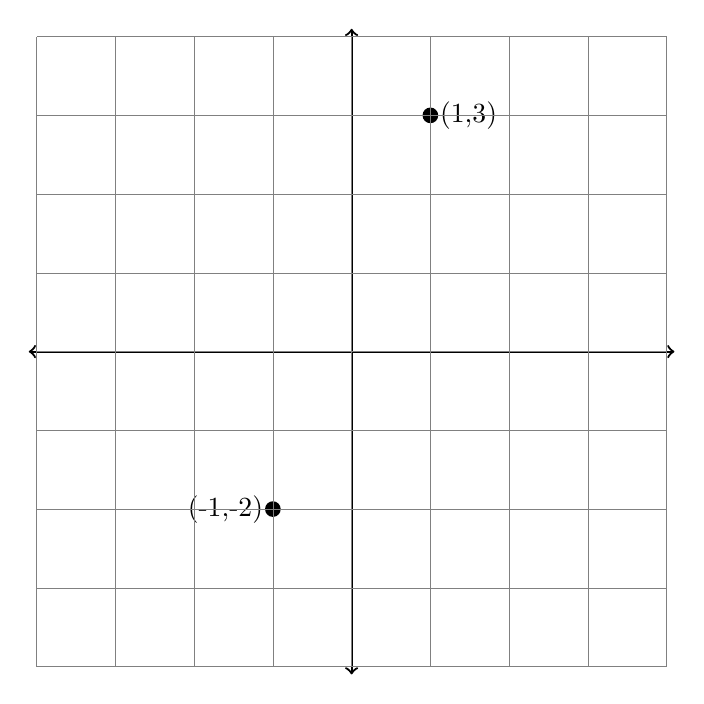
\begin{tikzpicture}
  % axis
  \draw[thick, <->] (0, -4.1) -- (0, 4.1);
  \draw[thick, <->] (-4.1, 0) -- (4.1, 0);
  \coordinate [circle, fill, inner sep=2pt] (a) at (-1,-2) ;
  \coordinate [circle, fill, inner sep=2pt] (b) at (1,3) ;
  \node [left] at (a) {(-1,-2)};
  \node [right] at (b) {(1,3)};
  % grid
  \draw[help lines, step = 1cm] (-4, -4) grid (4, 4);
  
\end{tikzpicture}

We can draw a right triangle and use the Pythagorean Theorem:

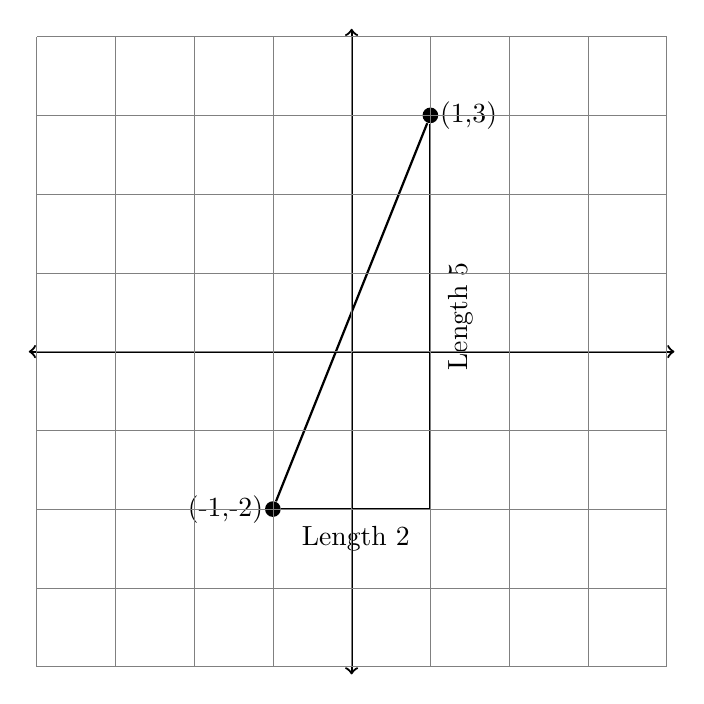
\begin{tikzpicture}
  % axis
  \draw[thick, <->] (0, -4.1) -- (0, 4.1);
  \draw[thick, <->] (-4.1, 0) -- (4.1, 0);
  \coordinate [circle, fill, inner sep=2pt] (a) at (-1,-2) ;
  \coordinate [circle, fill, inner sep=2pt] (b) at (1,3) ;
    \node [left] at (a) {(-1,-2)};
  \node [right] at (b) {(1,3)};
  \coordinate (c) at (1, -2);

  \draw [thick] (a) -- (b);
  \draw [thick] (a) -- node[outer sep = 3pt, below]{Length 2}(c);
  \draw [thick] (c) -- node[rotate=90, outer sep = 3pt, below]{Length 5}(b);
  \draw[help lines, step = 1cm] (-4, -4) grid (4, 4);
 
\end{tikzpicture}


The distance between the two points is $\sqrt{2^2 + 5^2} = \sqrt{29}
\approx 5.385165$. That is, you square the change in $x$ and add it to
the square of the change in $y$. The distance is the square root of
that sum.

\section{Distance in 3 Dimensions}

What if the point is in three dimensional space?  That is, you move 2
meters East, 8 meters North, and 4 meters up in the air. How far are
you from where you started?  You just square each, sum them and take the square root:
$\sqrt{2^2 + 8^2 + 4^2} = \sqrt{84} = 2\sqrt{21} \approx 9.165$ meters.

\begin{tikzpicture}
  \draw [thick, ->] (0,0,0) -- (9,0,0) node[outer sep = 1pt, right]{North} ; 
  \draw [thick, ->]  (0,0,0) -- (0,3,0) node[outer sep = 1pt, above]{Up} ; 
  \draw [thick, ->] (0,0,0) -- (0,0,4) node[outer sep = 1pt, below]{East} ; 

    \draw [dashed]  (8,0,0) -- node[outer sep = 1pt, right]{2}  (8,0,2); 

  \draw [dashed]  (0,0,2) -- node[outer sep = 1pt, below]{8} (8,0,2); 
  \draw [dashed]  (8,0,2) -- node[outer sep = 1pt, right]{4} (8,4,2); 
  \draw [thick]  (0,0,0) --  (8,4,2) node[circle, fill, inner sep=2pt]{}; 
  \node [left] at (5, 2.7, 1){$\sqrt{2^2 + 8^2 + 4^2} \approx 9.165$};

\end{tikzpicture}


\chapter{Congruence}
% Add: simple triangles
%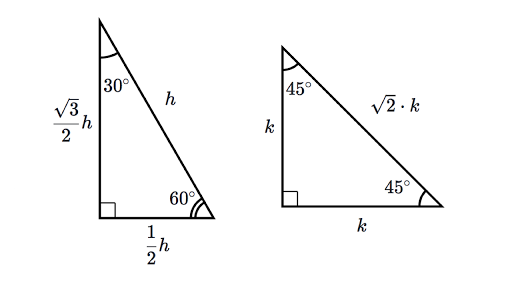
\includegraphics[width=0.8\textwidth]{KA_Special_Triangles.png}
Look at this picture of two geometric figures.

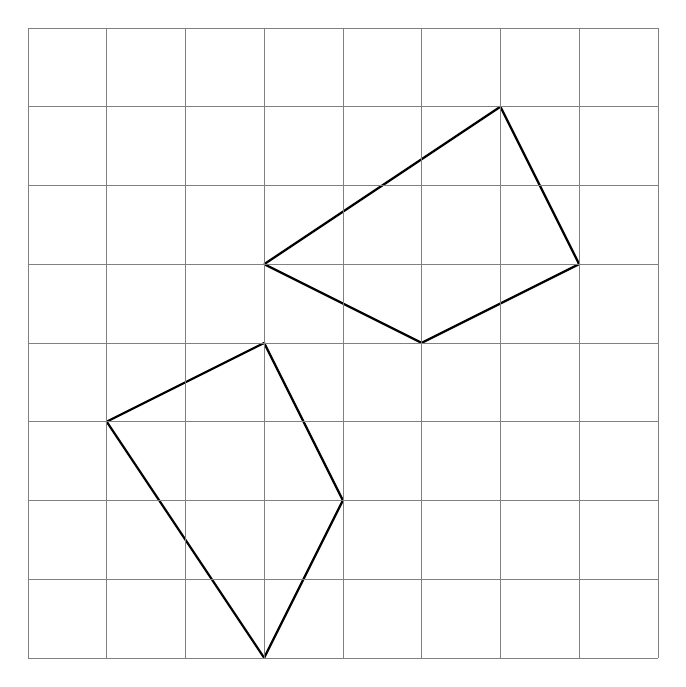
\begin{tikzpicture}
 
  	\draw [thick] (-1,-4) --  (0, -2);
	\draw [thick] (0,-2) --  (-1, 0) ;
	\draw [thick] (-1,0) --  (-3, -1); 
	\draw [thick] (-3,-1) --  (-1, -4);
	
	\draw [thick] (-1,1) --  (1, 0);
	\draw [thick] (1,0) --  (3, 1) ;
	\draw [thick] (3,1) --  (2, 3); 
	\draw [thick] (2,3) --  (-1, 1);

  \draw[help lines, step = 1cm] (-4, -4) grid (4, 4);
 
\end{tikzpicture}

They are the same shape, right? If you cut one out with scissors, it
would lay perfectly on top of the other. In geometry, we say they are
\emph{congruent}.

What is the official definition of ``congruent''? 
Two geometric figures are congruent if you can transform one into the other using
only rigid transformations. 

You might be wondering now, what are rigid transformations?
A transformation is \emph{Rigid} if it doesn't change the distances
between the points or the measure of the angles between the lines, they
form. These are all rigid transformations:
\begin{itemize}
\item Translations
\item Rotations
\item Reflections 
\end{itemize}

Once again imagine cutting out one figure with scissors and trying to match it with the second figure, your actions are rigid transformations:
\begin{itemize}
\item Translations - sliding the cutout left and right and up and down
\item Rotations	- rotating the cutout clockwise and counterclockwise
\item Reflection - flipping the piece of paper over
\end{itemize}

A transformation is rigid if it is some combination of translations, rotations, and reflections.

\section{Triangle Congruency}

If the sides of two triangles have the same length, the triangles must be congruent:

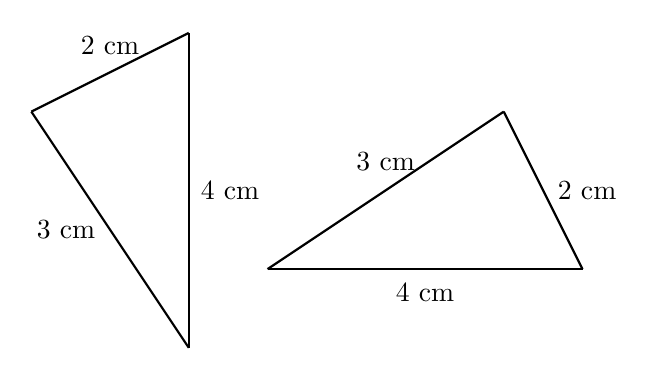
\begin{tikzpicture} 
  	\draw [thick] (-2,0) -- node[outer sep = 1pt, right]{4 cm}  (-2, 4) ;
	\draw [thick] (-2,4) --  node[outer sep = 3pt, above]{2 cm} (-4, 3); 
	\draw [thick] (-4,3) --  node[outer sep = 2pt, left]{3 cm} (-2, 0);
	
	\draw [thick] (-1,1) --  node[outer sep = 2pt, below]{4 cm}  (3, 1) ;
	\draw [thick] (3,1) --  node[outer sep = 2pt, right]{2 cm} (2, 3); 
	\draw [thick] (2,3) --  node[outer sep = 4pt, above]{3 cm} (-1, 1);
\end{tikzpicture}

To be precise, the Side-Side-Side Congruency Test says that two triangles are
congruent if three sides in one triangle are the same length as the
corresponding sides in the other. We usually refer to this as the SSS test.
% Explain with a^2 + b^2 = c^2

Note that two triangles with all three angles equal are not necessarily congruent.
For example, here are two triangles with the same interior angles, but they are
different sizes:

\begin{tikzpicture}
  \coordinate [circle, fill, inner sep=1pt] (a1) at (0,0) ;
  \coordinate [circle, fill, inner sep=1pt] (b1) at (4,0) ;
  \coordinate [circle, fill, inner sep=1pt] (c1) at (3,2) ;
  
   \coordinate [circle, fill, inner sep=1pt] (a2) at (5,0) ;
  \coordinate [circle, fill, inner sep=1pt] (b2) at (11,0) ;
  \coordinate [circle, fill, inner sep=1pt] (c2) at (9.5,3) ;
        \draw (a1) --   (b1);
        \draw (b1) -- (c1);
        \draw (c1)--  (a1);
        \pic [draw, "$63^\circ$", angle eccentricity=1.5] {angle = c1--b1--a1};
        \pic [draw, "$34^\circ$", angle eccentricity=2.0] {angle = b1--a1--c1};
        \pic [draw, "$83^\circ$", angle eccentricity=1.5] {angle = a1--c1--b1};

       \draw (a2) --  (b2);
        \draw (b2) -- (c2);
        \draw (c2)--  (a2);
        \pic [draw, "$63^\circ$", angle eccentricity=1.5] {angle = c2--b2--a2};
        \pic [draw, "$34^\circ$", angle eccentricity=2.0] {angle = b2--a2--c2};
        \pic [draw, "$83^\circ$", angle eccentricity=1.5] {angle = a2--c2--b2};

\end{tikzpicture}

These triangles are not congruent, but they are \emph{similar}. Meaning
 they have the same shape, but are not necessarily the same
size.

Therefore, if you know two angles of a triangle, you can calculate the third. So it makes sense
to say ``If two triangles have two angles that are equal, they are
similar triangles.''  And if two similar triangles have one side that
is equal in length, they must be the same size -- so they are
congruent. Thus, the Side-Angle-Angle Congruency Test says that
two triangles are congruent if two angles and one side match.

What if you know that two triangles have two sides that are the same
length and that the angle between them is also equal?

\begin{tikzpicture}
  \coordinate [circle, fill, inner sep=1pt] (a1) at (0,0) ;
  \coordinate [circle, fill, inner sep=1pt] (b1) at (4,0) ;
  \coordinate [circle, fill, inner sep=1pt] (c1) at (3,2) ;
  
  \coordinate [circle, fill, inner sep=1pt] (a2) at (5,0) ;
  \coordinate [circle, fill, inner sep=1pt] (b2) at (9,0) ;
  \coordinate [circle, fill, inner sep=1pt] (c2) at (8,2) ;
  
  \draw (a1) --  node[outer sep = 0.5pt, below]{4}  (b1);
  \draw [dashed] (b1) -- (c1);
  \draw (c1)--  node[outer sep = 5pt, above]{3.5} (a1);
  \pic [draw, "$34^\circ$", angle eccentricity=2.0] {angle = b1--a1--c1};

  \draw (a2) --  node[outer sep = 0.5pt, below]{4}  (b2);
  \draw [dashed] (b2) -- (c2);
  \draw (c2)--  node[outer sep = 5pt, above]{3.5} (a2);
  \pic [draw, "$34^\circ$", angle eccentricity=2.0] {angle = b2--a2--c2};
\end{tikzpicture}

Yes, they must be congruent. This is the Side-Angle-Size Congruency Test.

What if the angle isn't the one between the two known sides? If it is
a right angle, you can be certain the two triangles are congruent.
(How do I know? Because the Pythagorean Theorem tells us that we can
calculate the length of the third side. There is only one possibility,
thus all three sides must be the same length.)

\begin{tikzpicture}
  \coordinate [circle, fill, inner sep=1pt] (a1) at (0,0) ;
  \coordinate [circle, fill, inner sep=1pt] (b1) at (4,0) ;
  \coordinate [circle, fill, inner sep=1pt] (c1) at (4,2) ;
  
   \coordinate [circle, fill, inner sep=1pt] (a2) at (5,0) ;
  \coordinate [circle, fill, inner sep=1pt] (b2) at (9,0) ;
  \coordinate [circle, fill, inner sep=1pt] (c2) at (9,2) ;
        \draw (a1) --  node[outer sep = 0.5pt, below]{3.5}  (b1);
        \draw [dashed] (b1) -- (c1);
        \draw (c1)--  node[outer sep = 5pt, above]{4} (a1);
        \pic [draw] {right angle = a1--b1--c1};

        \draw (a2) --  node[outer sep = 0.5pt, below]{3.5}  (b2);
        \draw [dashed] (b2) -- (c2);
        \draw (c2)--  node[outer sep = 5pt, above]{4} (a2);
        \pic [draw] {right angle = a2--b2--c2};
\end{tikzpicture}

In this case, the third side of each triangle must be $\sqrt{4^2 - 3.5^2} \approx 1.9$.

What if the know angle is less than $90^\circ$? \emph{The triangles
  are not necessarily congruent.} For example, let's say that there are
two triangles with sides of length 5 and 7 and that the corresponding
angle (at the end of the side of length 7) on each is $45^\circ$. Two
different triangles satisfy this:

\begin{tikzpicture}
  \coordinate [circle, fill, inner sep=1pt] (a1) at (0,0) ;
  \coordinate [circle, fill, inner sep=1pt] (b1) at (7,0) ;
  \coordinate [circle, fill, inner sep=1pt] (c1) at (4,3) ;
  \coordinate [circle, fill, inner sep=1pt] (a2) at (8,0) ;
  \coordinate [circle, fill, inner sep=1pt] (b2) at (15,0) ;
  \coordinate [circle, fill, inner sep=1pt] (c2) at (11,4) ;
  \draw (a1) --  node[outer sep = 0.5pt, below]{7}  (b1);
  \draw [dashed] (b1) -- (c1);
  \draw (c1)--  node[outer sep = 5pt, above]{5}(a1);
  \pic [draw, "$45^\circ$", angle eccentricity=1.5] {angle = c1--b1--a1};
  \draw (a2) --  node[outer sep = 0.5pt, below]{7}  (b2);
  \draw [dashed] (b2) -- (c2);
  \draw (c2)--  node[outer sep = 5pt, above]{5} (a2);
  \pic [draw, "$45^\circ$", angle eccentricity=1.5] {angle = c2--b2--a2};
\end{tikzpicture}

Let's see this another way by laying one triangle on top of the other:

\begin{tikzpicture}
  \coordinate [circle, fill, inner sep=1pt] (a1) at (0,0) ;
  \coordinate [circle, fill, inner sep=1pt] (b1) at (7,0) ;
  \coordinate [circle, fill, inner sep=1pt] (c1) at (4,3) ;
  \coordinate [circle, fill, inner sep=1pt] (c2) at (3,4) ;
  \coordinate (d) at (2,5);
  \coordinate (e) at (3.5,3.5);

  \draw (a1) --  node[outer sep = 0.5pt, below]{7}  (b1);
  \draw [dashed,->] (b1) -- (d);
  \draw [dashed] (a1) -- (e);
  \draw (c1)--  node[outer sep = 5pt, below]{5}(a1);
  \draw (c2)--  node[outer sep = 5pt, above]{5}(a1);
  \pic [draw, "$45^\circ$", angle eccentricity=1.5] {angle = c1--b1--a1};
   \pic [draw, angle radius=8] {right angle = b1--e--a1};
\end{tikzpicture}


So there is \emph{not} a general Side-Side-Angle Congruency Test.

Here, then, is the list of common congruency tests:
\begin{itemize}
\item Side-Side-Side: All three sides have the same measure
\item Side-Angle-Angle: Two angles and one side have the same measure
\item Side-Angle-Side: Two sides and the angle between them have the same measure
\item Side-Side-Right: They are right triangles and have two sides have the same measure
\end{itemize}

\begin{Exercise}[title={Congruent Triangles}, label=con_triangles]
  Ted is terrible at drawing triangles: he always draws them exactly
  the same. Fortunately, he has marked these diagrams with the sides
  and angles that he measured. For each pair of triangles, write if
  you know them to be congruent and which congruency test proves
  it. For example:

\begin{tikzpicture}[scale=0.7]
  \coordinate [circle, fill, inner sep=1pt] (a1) at (0,1) ;
  \coordinate [circle, fill, inner sep=1pt] (b1) at (5,0) ;
  \coordinate [circle, fill, inner sep=1pt] (c1) at (4,2) ;
  
  \coordinate [circle, fill, inner sep=1pt] (a2) at (6,1) ;
  \coordinate [circle, fill, inner sep=1pt] (b2) at (11,0) ;
  \coordinate [circle, fill, inner sep=1pt] (c2) at (10,2) ;
  \draw (a1) --  node[outer sep = 0.5pt, below]{3.5}  (b1);
  \draw (b1) -- node[outer sep = 2pt, right]{4} (c1);
  \draw (c1)--  node[outer sep = 2pt, above]{} (a1);
  \pic [draw,  "$120^\circ$", angle eccentricity=2.0] {angle = c1--b1--a1};

  \draw (a2) --  node[outer sep = 0.5pt, below]{3.5}  (b2);
  \draw  (b2) -- node[outer sep = 2pt, right]{4} (c2);
  \draw (c2) -- node[outer sep = 2pt, above]{} (a2);
  \pic [draw,  "$120^\circ$",, angle eccentricity=2.0] {angle = c2--b2--a2};
\end{tikzpicture}

  (These drawings are clearly not accurate, but you are told the measurements are.) The answer is ``Congruent by the Side-Angle-Side test.''

  \begin{multicols}{2}

\begin{tikzpicture}[scale=0.6]
  \coordinate [circle, fill, inner sep=1pt] (a1) at (0,1) ;
  \coordinate [circle, fill, inner sep=1pt] (b1) at (5,0) ;
  \coordinate [circle, fill, inner sep=1pt] (c1) at (4,2) ;
  
  \coordinate [circle, fill, inner sep=1pt] (a2) at (6,1) ;
  \coordinate [circle, fill, inner sep=1pt] (b2) at (11,0) ;
  \coordinate [circle, fill, inner sep=1pt] (c2) at (10,2) ;
  \draw (a1) --  node[outer sep = 0.5pt, below]{3.5}  (b1);
  \draw (b1) -- node[outer sep = 2pt, right]{} (c1);
  \draw (c1)--  node[outer sep = 2pt, above]{6} (a1);
  \pic [draw,  "$90^\circ$", angle eccentricity=2.0] {angle = c1--b1--a1};

  \draw (a2) --  node[outer sep = 0.5pt, below]{3.5}  (b2);
  \draw  (b2) -- node[outer sep = 2pt, right]{} (c2);
  \draw (c2) -- node[outer sep = 2pt, above]{6} (a2);
  \pic [draw,  "$90^\circ$",, angle eccentricity=2.0] {angle = c2--b2--a2};
\end{tikzpicture}

\hspace{3cm}

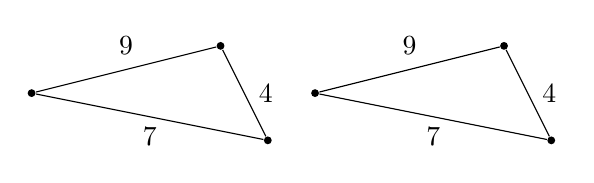
\begin{tikzpicture}[scale=0.6]
  \coordinate [circle, fill, inner sep=1pt] (a1) at (0,1) ;
  \coordinate [circle, fill, inner sep=1pt] (b1) at (5,0) ;
  \coordinate [circle, fill, inner sep=1pt] (c1) at (4,2) ;
  
  \coordinate [circle, fill, inner sep=1pt] (a2) at (6,1) ;
  \coordinate [circle, fill, inner sep=1pt] (b2) at (11,0) ;
  \coordinate [circle, fill, inner sep=1pt] (c2) at (10,2) ;
  \draw (a1) --  node[outer sep = 0.5pt, below]{7}  (b1);
  \draw (b1) -- node[outer sep = 2pt, right]{4} (c1);
  \draw (c1)--  node[outer sep = 2pt, above]{9} (a1);

  \draw (a2) --  node[outer sep = 0.5pt, below]{7}  (b2);
  \draw  (b2) -- node[outer sep = 2pt, right]{4} (c2);
  \draw (c2) -- node[outer sep = 2pt, above]{9} (a2);
\end{tikzpicture}


\begin{tikzpicture}[scale=0.6]
  \coordinate [circle, fill, inner sep=1pt] (a1) at (0,1) ;
  \coordinate [circle, fill, inner sep=1pt] (b1) at (5,0) ;
  \coordinate [circle, fill, inner sep=1pt] (c1) at (4,2) ;
  
  \coordinate [circle, fill, inner sep=1pt] (a2) at (6,1) ;
  \coordinate [circle, fill, inner sep=1pt] (b2) at (11,0) ;
  \coordinate [circle, fill, inner sep=1pt] (c2) at (10,2) ;
  \draw (a1) --  node[outer sep = 0.5pt, below]{7}  (b1);
  \draw (b1) -- node[outer sep = 2pt, right]{} (c1);
  \draw (c1)--  node[outer sep = 2pt, above]{} (a1);
  \pic [draw,  "$35^\circ$",, angle eccentricity=2.0] {angle = c1--b1--a1};
  \pic [draw,  "$62^\circ$",, angle eccentricity=2.0] {angle = b1--a1--c1};

  \draw (a2) --  node[outer sep = 0.5pt, below]{7}  (b2);
  \draw  (b2) -- node[outer sep = 2pt, right]{} (c2);
  \draw (c2) -- node[outer sep = 2pt, above]{} (a2);
  \pic [draw,  "$35^\circ$",, angle eccentricity=2.0] {angle = c2--b2--a2};
  \pic [draw,  "$62^\circ$",, angle eccentricity=2.0] {angle = b2--a2--c2};

\end{tikzpicture}

\hspace{3cm}


\begin{tikzpicture}[scale=0.6]
  \coordinate [circle, fill, inner sep=1pt] (a1) at (0,1) ;
  \coordinate [circle, fill, inner sep=1pt] (b1) at (5,0) ;
  \coordinate [circle, fill, inner sep=1pt] (c1) at (4,2) ;
  
  \coordinate [circle, fill, inner sep=1pt] (a2) at (6,1) ;
  \coordinate [circle, fill, inner sep=1pt] (b2) at (11,0) ;
  \coordinate [circle, fill, inner sep=1pt] (c2) at (10,2) ;
  \draw (a1) --  node[outer sep = 0.5pt, below]{8}  (b1);
  \draw (b1) -- node[outer sep = 2pt, right]{6} (c1);
  \draw (c1)--  node[outer sep = 2pt, above]{} (a1);
  \pic [draw,  "$28^\circ$",, angle eccentricity=2.0] {angle = b1--a1--c1};

  \draw (a2) --  node[outer sep = 0.5pt, below]{8}  (b2);
  \draw  (b2) -- node[outer sep = 2pt, right]{6} (c2);
  \draw (c2) -- node[outer sep = 2pt, above]{} (a2);
  \pic [draw,  "$28^\circ$",, angle eccentricity=2.0] {angle = b2--a2--c2};

\end{tikzpicture}


\end{multicols}
\end{Exercise}

\begin{Answer}[ref=con_triangles]
\begin{multicols}{2}
Congruent by the Side-Side-Right Congruency Test.

Congruent by the Side-Side-Side Congruency Test.

Congruent by the Side-Angle-Angle Congruency Test.

We don't know if they are congruent. The measured angle is not between the measured sides.

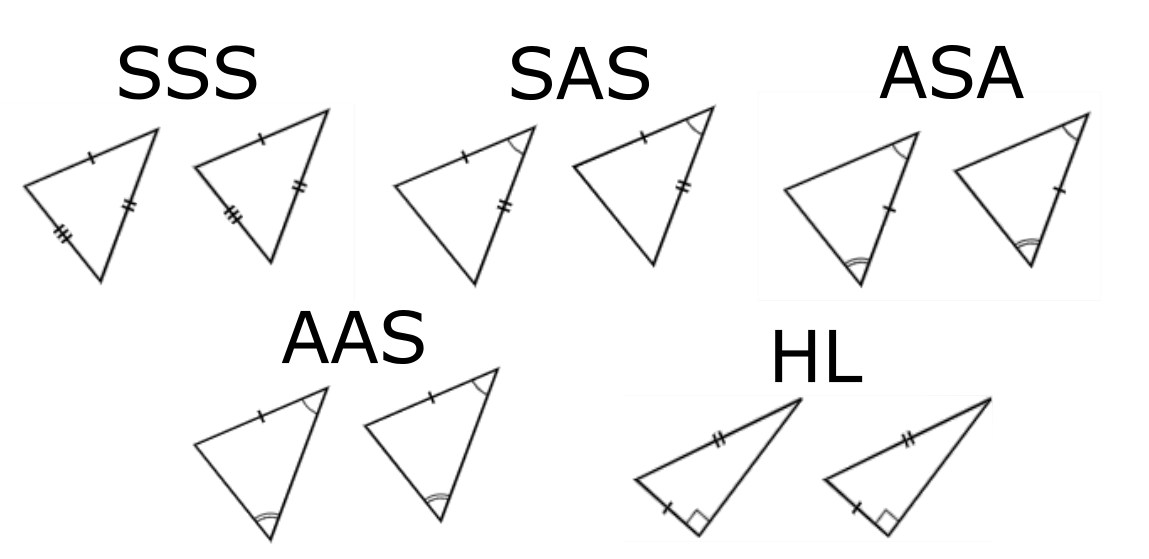
\includegraphics[width=0.8\textwidth]{Triangle_Congruence.png}
\end{multicols}

\end{Answer}




\chapter{Vectors}

We have talked a some about forces, but in the calculations that we
have done, we have only talked about the magnitude of a force. It is
equally important to talk about its direction. To do the math on
things with a magnitude and a direction (like forces), we need vectors.\index{vectors}

For example, if you jump out of a plane (hopefully with a parachute), 
several forces with different magnitudes and directions will be acting upon 
you. Gravity will push you straight down. That force will be proportional to your weight.
If there were a wind from the west, it would push you toward the east. That force
will be proportional to the square of the speed of the wind and approximately proportional to 
your size. Once you are falling, there will be resistance from the air 
that you are pushing through -- that force will point in the opposite direction
from the direction you are moving and will be proportional to the square of your
speed.

To figure out the net force (which will tell us how we will accelerate), we will 
need to add these forces together. So we need to learn to do math with vectors.

\section{Adding Vectors}

A vector is typically represented as a list of numbers, with each
number representing a particular dimension. For example, if I am
creating a 3-dimensional vector representing a force, it will have
three numbers representing the amount of force in each of the three
axes. For example, if a force of one newton is in the direction of the
$x$-axis, I might represent the vector as $v = [1, 0, 0]$. 
Another vector might be $u = [0.5, 0.9, 0.7]$ \index{vectors!adding}

\tdplotsetmaincoords{80}{130} 
\begin{tikzpicture} [scale=4, tdplot_main_coords, axis/.style={->,sdkblue}, 
vector/.style={-stealth,black,very thick}, 
vector guide/.style={dashed,sdkblue}]

%standard tikz coordinate definition using x, y, z coords
\coordinate (O) at (0,0,0);

%draw axes
\draw[axis] (0,0,0) -- (1.5,0,0) node[anchor=north east]{$x$};
\draw[axis] (0,0,0) -- (0,0.9,0) node[anchor=north west]{$y$};
\draw[axis] (0,0,0) -- (0,0,0.9) node[anchor=south]{$z$};

%draw a vector from O to P
\draw[vector] (O) -- (1,0,0);
\draw[vector] (O) -- (0.5,0.9,0.7);
\draw (0.2,0.0,0.05) node[left] {v};
\draw (0.2,0.35,0.3) node[right] {u};

\draw[vector guide] (0.5,0,0) -- (0.5,0.9,0);
\draw[vector guide] (0.0,0.9,0) -- (0.5,0.9,0);
\draw[vector guide] (0.5,0.9,0) -- (0.5,0.9,0.7);
\end{tikzpicture}

Thinking visually, when we add to vectors, we put the starting point 
second vector at the ending point of the first vector.


\tdplotsetmaincoords{80}{130} 
\begin{tikzpicture} [scale=4, tdplot_main_coords, axis/.style={->,sdkblue}, 
light vector/.style={-stealth,dashed,very thick, black}, 
vector/.style={-stealth,black,very thick}, 
vector guide/.style={dashed,sdkblue}]

%standard tikz coordinate definition using x, y, z coords
\coordinate (O) at (0,0,0);

%draw axes
\draw[axis] (0,0,0) -- (1.5,0,0) node[anchor=north east]{$x$};
\draw[axis] (0,0,0) -- (0,0.9,0) node[anchor=north west]{$y$};
\draw[axis] (0,0,0) -- (0,0,0.9) node[anchor=south]{$z$};

%draw a vector from O to P
\draw[light vector] (0,0,0) -- (0.5,0.9,0.7);
\draw[light vector] (0.5, 0.9, 0.7) -- (1.5, 0.9, 0.7);
\draw[vector] (0,0,0) -- (1.5,0.9,0.7) node[left] {u + v};
\draw (0.7,0.9,0.75) node[left] {v};
\draw (0.2,0.35,0.3) node[right] {u};

\draw[vector guide] (0.5,0,0) -- (0.5,0.9,0);
\draw[vector guide] (0.0,0.9,0) -- (0.5,0.9,0);
\draw[vector guide] (0.5,0.9,0) -- (0.5,0.9,0.7);
\draw[vector guide] (0.5,0.9,0) -- (1.5,0.9,0.0);
\draw[vector guide] (1.5,0.9,0.0) -- (1.5,0.9,0.7);
\draw[vector guide] (1.5,0.0,0.0) -- (1.5,0.9,0.0);

\end{tikzpicture}

If you know the vectors, you will just add them element-wise:

$$ u + v = [0.5, 0.9, 0.7] + [1.0, 0.0, 0.0] = [1.5, 0.9. 0.7] $$

These vectors have 3 components, so we say they are \newterm{3-dimensional}. 
Vectors can have any number of components. For example, the vector
 $[-12.2, 3, \pi, 10000]$ is 4-dimensional.

 You can only add two vectors if they have the same dimension.

 $$ [12, -4] + [-1, 5] = [11,1] $$

 Addition is commutative: If you have two vectors $a$ and $b$, then
 $a + b$ is the same as $b + a$.

 Addition is also associative: If you have three vectors $a$, $b$, and $c$,
 it doesn't matter which order you add them in. 
 That is, $a + (b + c) = (a + b) + c$.

 A 1-dimensional vector is just a number.  We say it is a 
 \newterm{scalar}, not a vector.

 \begin{Exercise}[title={Adding vectors}, label=adding_vectors]
Add the following vectors:
\begin{itemize}
    \item $[1, 2, 3] + [4, 5, 6]$
    \item $[-1, -2, -3, -4] + [4, 5, 6, 7]$
    \item $[\pi, 0, 0] + [0, \pi, 0] + [0, 0, \pi]$
\end{itemize}
\end{Exercise}
\begin{Answer}[ref=adding_vectors]
    \begin{itemize}
        \item $[1, 2, 3] + [4, 5, 6] = [5, 7, 9]$
        \item $[-1, -2, -3, -4] + [4, 5, 6, 7] = [3, 3, 3, 3]$
        \item $[\pi, 0, 0] + [0, \pi, 0] + [0, 0, \pi] = [\pi, \pi, \pi]$ 
    \end{itemize}
\end{Answer}

    \begin{Exercise}[title={Adding Forces}, label=adding_forces]
        You are adrift in space. You are near two different stars. 
        The gravity of one star is pulling you towards it with a 
        force of $[4.2, 5.6, 9.0]$ newtons.
        The gravity of the other star is pulling you towards it with
        a force of $[-100.2, 30.2, -9.0]$ newtons. What is the net force?
        \end{Exercise}
        \begin{Answer}[ref=adding_forces]
            To get the net force, you add the two forces:

            $$F = [4.2, 5.6, 9.0] + [-100.2, 30.2, -9.0] = [-96, 35.8, 0.0] \text{ newtons}$$
   
\end{Answer}

\section{Multiplying a vector with a scalar}

It is not uncommon to multiply a vector by a scalar.  For example, a rocket engine
might have a force vector $v$.  If you fire 9 engines in the exact same direction,
the resulting force vector would be $9v$.\index{vectors!multipying by a scalar}

Visually, when we multiply a vector $u$ by a scalar $a$, we get a new vector that
goes in the same direction as $u$ but has a magnitude $a$ times as long as $u$.

\tdplotsetmaincoords{80}{130} 
\begin{tikzpicture} [scale=3, tdplot_main_coords, axis/.style={->,sdkblue}, 
vector/.style={-stealth,black,very thick}, 
vector guide/.style={dashed,sdkblue}]

%standard tikz coordinate definition using x, y, z coords
\coordinate (O) at (0,0,0);

%draw axes
\draw[axis] (0,0,0) -- (1.6,0,0) node[anchor=north east]{$x$};
\draw[axis] (0,0,0) -- (0,2.8,0) node[anchor=north west]{$y$};
\draw[axis] (0,0,0) -- (0,0,1.9) node[anchor=south]{$z$};

%draw a vector from O to P
\draw[vector] (O) -- (0.5,0.9,0.7);
\draw (0.2,0.35,0.3) node[right] {$u$};

\draw[vector] (O) -- (1.5,2.7,2.1) node[right] {$3u$};


\draw[vector guide] (0.5,0,0) -- (0.5,0.9,0);
\draw[vector guide] (0.0,0.9,0) -- (0.5,0.9,0);
\draw[vector guide] (0.5,0.9,0) -- (0.5,0.9,0.7);

\draw[vector guide] (1.5,0,0) -- (1.5,2.7,0);
\draw[vector guide] (0.0,2.7,0) -- (1.5,2.7,0);
\draw[vector guide] (1.5,2.7,0) -- (1.5,2.7,2.1);
\end{tikzpicture}

When you multiply a vector by a scalar, you just multiply each of the components by the scalar:

$$ 3 \times [0.5, 0.9, 0.7] = [1.5, 2.7, 3.6] $$

\begin{Exercise}[title={Multiplying a vector and a scalar}, label=mult_scalar]
    Simplify the following expressions:
    \begin{itemize}
        \item $2 \times [1, 2, 3]$
        \item $[-1, -2, -3, -4] \times -2$
        \item $\pi[\pi, 2\pi, 3\pi]$
    \end{itemize}
    \end{Exercise}
    \begin{Answer}[ref=mult_scalar]
        \begin{itemize}
            \item $2 \times [1, 2, 3] = [2, 4, 6]$
            \item $[-1, -2, -3, -4] \times -3 = [3, 6, 9, 12]$
            \item $\pi[\pi, 2\pi, 3\pi]  = \pi^2, 2\pi^2, 3\pi^2]$ 
        \end{itemize}
    \end{Answer}

Note that when you multiply a vector times a negative number, the new vector points 
in the opposite direction.

\tdplotsetmaincoords{80}{130} 
\begin{tikzpicture} [scale=5, tdplot_main_coords, axis/.style={->,sdkblue}, 
vector/.style={-stealth,black,very thick}, 
vector guide/.style={dashed,sdkblue}]

%standard tikz coordinate definition using x, y, z coords
\coordinate (O) at (0,0,0);

%draw axes
\draw[axis] (0,0,0) -- (0.55,0,0) node[anchor=north east]{$x$};
\draw[axis] (0,0,0) -- (0,0.95,0) node[anchor=north west]{$y$};
\draw[axis] (0,0,0) -- (0,0,0.6) node[anchor=south]{$z$};

%draw a vector from O to P
\draw[vector] (O) -- (0.5,0.9,0.7);
\draw (0.2,0.36,0.3) node[right] {$u$};

\draw[vector] (O) -- (-0.25,-0.45,-0.35) node[right] {$(-0.5)u$};

\draw[vector guide] (0.5,0,0) -- (0.5,0.9,0);
\draw[vector guide] (0.0,0.9,0) -- (0.5,0.9,0);
\draw[vector guide] (0.5,0.9,0) -- (0.5,0.9,0.7);

\draw[vector guide] (-0.25,0,0) -- (-0.25,-0.45,0);
\draw[vector guide] (0,0,0) -- (-0.25,0,0);
\draw[vector guide] (0.0,-0.45,0) -- (-0.25,-0.45,0);
\draw[vector guide] (0,0,0) -- (0,-0.45,0);

\draw[vector guide] (-.25,-0.45,0) -- (-0.25,-0.45,-0.35);
\end{tikzpicture}

\section{Vector Subtraction}

As you might guess, when you subtract one vector from another, 
you just do element-wise subtraction:\index{vectors!subtraction}

$$[4,2,0] - [3,-2, 9] = [1, 4, -9]$$

So, $u - v = u + (-1v)$.

So visually, you reverse the one that is being subtracted:


\tdplotsetmaincoords{80}{130} 
\begin{tikzpicture} [scale=5, tdplot_main_coords, axis/.style={->,sdkblue}, 
light vector/.style={-stealth,dashed,very thick, black}, 
vector/.style={-stealth,black,very thick}, 
vector guide/.style={dashed,sdkblue}]

%standard tikz coordinate definition using x, y, z coords
\coordinate (O) at (0,0,0);

%draw axes
\draw[axis] (0,0,0) -- (0.55,0,0) node[anchor=north east]{$x$};
\draw[axis] (0,0,0) -- (0,1.0,0) node[anchor=north west]{$y$};
\draw[axis] (0,0,0) -- (0,0,0.75) node[anchor=south]{$z$};

%draw a vector from O to P
\draw[light vector] (0,0,0) -- (0.5,0.9,0.7);
\draw[light vector] (0.5, 0.9, 0.7) -- (-0.5, 0.9, 0.7);
\draw[vector] (0,0,0) -- (-0.5,0.9,0.7) node[right] {u - v};
\draw (0.1,0.9,0.75) node[left] {-v};
\draw (0.29,0.34,0.32) node[right] {u};

\draw[vector guide] (0.5,0,0) -- (0.5,0.9,0);
\draw[vector guide] (0.0,0.9,0) -- (0.5,0.9,0);
\draw[vector guide] (0.5,0.9,0) -- (0.5,0.9,0.7);
\draw[vector guide] (0.5,0.9,0) -- (-0.5,0.9,0.0);
\draw[vector guide] (-0.5,0.9,0.0) -- (-0.5,0.9,0.7);
\draw[vector guide] (-0.5,0.0,0.0) -- (-0.5,0.9,0.0);
\draw[vector guide] (0,0.0,0.0) -- (-0.5,0.0,0.0);

\end{tikzpicture}

\section{Magnitude of a Vector}

The \newterm{magnitude} of a vector is just its length. We write the 
magnitude of a vector $v$ as $|v|$.\index{vectors!magnitude of}

We compute the magnitude using the pythagorean theorem.  If $v = [3,4,5]$, 
then

\begin{equation*}
    |v| = \sqrt{3^2 + 4^2 + 5^2} = \sqrt{50} \approx 7.07
\end{equation*}

(You might notice that the notation for the magnitude is exactly like the notation for absolute value.
If you think of a scalar as a 1-dimensional vector, the absolute value and the magnitude are the same. 
For example, the absolute value of -5 is 5.  If you take the magnitude of the one-dimenional vector $[-5]$,
you get $\sqrt{25} = 5$.)

Notice that if you scale up a vector, its magnitude scales by the same amount.  For example:

\begin{equation*}
|7[3,4,5]| = 7 \sqrt{50} \approx 7 \times 7.07    
\end{equation*}

The rule then is: If you have any vector $v$ and any scalar $a$:
\begin{equation*}
    |a v| = |a| |v|
\end{equation*}


\begin{Exercise}[title={Magnitude of a Vector}, label=vector_mag]
    Find the magnitude of the following vectors:
    \begin{itemize}
        \item $[1, 1, 1]$
        \item $[-5, -5, -5]$ (that is the same as $-5 \times [1, 1, 1]$)
        \item $[3, 4, -4] + [-2, -3, 5]$
    \end{itemize}
    \end{Exercise}
    \begin{Answer}[ref=vector_mag]
        \begin{itemize}
            \item $|[1, 1, 1]| = \sqrt{3} \approx 1.73 $
            \item $|[-5, -5, -5]| = |-5 \times [1,1,1]| = 5 \sqrt{3} \approx 8.66$
            \item $|[3, 4, 5] + [-2, -3, -4]| = | [1,1,1] | = \sqrt{3} \approx 1.73$ 
        \end{itemize}
    \end{Answer}

\section{Vectors in Python}

NumPy is a library that allows you to work with vectors in Python.  
You might need to install it on your computer. This is done with \pyfunction{pip}. 
\pyfunction{pip3} installs things specifically for Python 3.\index{vectors!in python}

\begin{Verbatim}
pip3 install NumPy
\end{Verbatim}

We can think of a vector as a list of numbers.  
There are also grids of numbers known as \newterm{matrices}. NumPy deals with both in the same way, 
so it refers to both of them as arrays.\index{NumPy}

The study of vectors and matrices is known as \newterm{Linear Algebra}. Some of the functions we need
are in a sublibrary of NumPy called \pyfunction{linalg}. \index{linalg}

As a convention, everyone who uses NumPy, imports it as \textit{np}. \index{np}

Create a file called \filename{first\_vectors.py}:

\begin{Verbatim}
import NumPy as np

# Create two vectors
v = np.array([2,3,4])
u = np.array([-1,-2,3])
print(f"u = {u}, v = {v}")

# Add them
w = v + u
print(f"u + v = {w}")

# Multiply by a scalar
w = v * 3
print(f"v * 3 = {w}")

# Get the magnitude
# Get the magnitude
mv = np.linalg.norm(v)
mu = np.linalg.norm(u)
print(f"|v| = {mv}, |u| = {mu}")
\end{Verbatim}

When you run it, you should see:

\begin{Verbatim}
> python3 first_vectors.py
u = [-1 -2  3], v = [2 3 4]
u + v = [1 1 7]
v * 3 = [ 6  9 12]
|v| = 5.385164807134504, |u| = 3.7416573867739413
\end{Verbatim}

\subsection{Formatting Floats}

The numbers 5.385164807134504 and 3.7416573867739413 are pretty long.  You probably want it 
rounded off after a couple of decimal places.

Numbers with decimal places are called \newterm{floats}. In the placeholder for your float, you 
can specify how you want it formatted, including the number of decimal places.

Change the last line to look like this:\index{floats!formatting}
\begin{Verbatim}
    print(f"|v| = {mv:.2f}, |u| = {mu:.2f}")
\end{Verbatim}

When you run the code, it will be neatly rounded off to two decimal places:
\begin{Verbatim}
|v| = 5.39, |u| = 3.74
\end{Verbatim}

\chapter{The Dot Product}

If you have two vectors $u = [u_1, u_2, \dots, w_n]$ and $v = [v_1, v_2,\dots, v_n]$ , 
we define the \newterm{dot product} $u \cdot v$ as 
\begin{equation*}
     u \cdot v = (u_1 \times v_1) + (u_2 \times v_2) + \dots + (u_n \times v_n)
\end{equation*} 

So, for example, 
\begin{equation*}
    [2,4, -3] \cdot [5, -1, 1] = 2 \times 5 + 4 \times -1 + -3 \times 1 = 3
\end{equation*}\index{dot product}

I know, this doesn't seem like a very powerful idea, but dot products actually turn out to 
be \emph{incredibly} useful.  The enormous GPUs that let video games render scenes so quickly? 
They are primarily designed to do huge numbers of dot products at mind-boggling speeds. 

\begin{Exercise}[title={Basic dot products}, label=dot_products]
    Compute the dot product of each pair of vectors:
    \begin{itemize}
        \item $[1, 2, 3]$, $[4, 5, -6]$
        \item $[\pi, 2\pi]$, $[2, -1]$
        \item $[0,0,0,0]$, $[10,10,10,10]$
    \end{itemize}
\end{Exercise}
\begin{Answer}[ref=dot_products]
        \begin{itemize}
            \item $[1, 2, 3] \cdot [4, 5, -6] = 4 + 10 - 18 = -4$
            \item $[\pi, 2\pi] \cdot [2, -1] = 2\pi - 2\pi = 0$
            \item $[0,0,0,0] \cdot [10,10,10,10] = 0 + 0 + 0 + 0 = 0$ 
        \end{itemize}
\end{Answer}

\section{Properties of the dot product}

Sometimes I need an easy way to say ``The vector of appropriate length that is filled with zeros.''
I will use the notation $\vec{0}$ to represent this. Then, for any vector $v$, this is true:

$$v \cdot \vec{0} = 0$$

The dot product is commutative:

$$v \cdot u = u \cdot v$$

The dot product of a vector with itself is its magnitude squared:

$$ v \cdot v = |v|^2 $$

If you have a scalar $a$ then:

    $$(v) \cdot (a u) = a (v \cdot u)$$

So, if $v$ and $w$ are vectors that go in the same direction,

    $$v \cdot w = |v| |w|$$

If $v$ and $w$ are vectors that go in opposite directions,

    $$v \cdot w = -|v| |w|$$

\section{Cosines and dot products}

Here is the property of dot products is what makes them so useful: 
If you have two vectors $v$ and $u$,

$$v \cdot u = |v| |u| \cos \theta$$

where $\theta$ is the angle between them.

So, for example, if two vectors $v$ and $u$ are perpendicular, the angle between them is $\pi/2$.  
The cosine of $\pi/2$ is 0: The dot product of any two perpendicular vectors is always 0. In fact, if 
the dot product of two non-zero vectors is 0, the vectors \textit{must be} perpendicular.

\begin{Exercise}[title={Using dot products}, label=cos_dot_products]
    What is the angle between these each pair of vectors:
    \begin{itemize}
        \item $[1, 0]$, $[0, 1]$
        \item $[3,4]$, $[4,3]$
    \end{itemize}
\end{Exercise}
\begin{Answer}[ref=cos_dot_products]
        \begin{itemize}
            \item $[1,0] \cdot [0,1] = 0$.  The angle must be $\pi/2$.
            \item $[3,4] \cdot [4, 3] = 24$. $|[3,4]| |[4,3]| \cos(\theta) = 24$. 
            $\cos(\theta) = \frac{24}{(5)(5)}$. $\theta = \arccos(\frac{24}{25}) \approx 0.284 \text{ radians}$.
        \end{itemize}
\end{Answer}

If you have two non-zero vectors $v$ and $u$, you can always compute the angle between them:\index{vectors!angle between}

$$\theta = \arccos(\frac{v \cdot u}{|v| |u|})$$

\section{Dot products in Python}

numpy will let you do dot products using the the symbol @.  Open \filename{first\_vectors.py} 
and add the following to the end:

\begin{Verbatim}
    # Take the dot product
    d = v @ u
    print("v @ u =", d)
    
    # Get the angle between the vectors
    a = np.arccos(d / (mv * mu))
    print(f"The angle between u and v is {a * 180 / np.pi:.2f} degrees")    
\end{Verbatim}

When you run it you should get:
\begin{Verbatim}
v @ u = 4
The angle between u and v is 78.55 degrees
\end{Verbatim}

\section{Work and Power}

Earlier, we mentioned that mechanical work is the product of the 
force you apply to something and the amount it moves. For example, if you 
push a train with a force of 10 newtons as it moves 5 meters, you have done 15 joules of work.

What if you try to push the train sideways? That is, it moves down the track 5 meters, 
but you push it as if you were trying to derail it -- perpendicular to its motion.  
You have done no work because the train didn't move at all in the direction you were pushing.

Now that you know about dot products, I can tell you the whole truth: The work you do is the dot
product of the force vector you apply and the displacement vector of the train. (The displacement
vector is the vector that tells how the train moved while you pushed it.) \index{work}

Similary, we mentioned that power is the product of the force you apply and the velocity of the
mass you are applying it to. It is actually the dot product of the force vector and the velocity vector.\index{power}

For example, if you are pushing sled with a force of 10 newtons and it is moving 2 meters per second, 
but your push is 20 degrees off, you aren't transferring 20 watts of power to the sled.  
You are transferring $10 \times 2 \times \cos(20 \text{ degrees}) \approx 18.8$ watts of power.

\graphicspath{{../../Modules/Functions/}}
\chapter{Functions and Their Graphs}

You can think of a function as a machine: you put something into the
machine, it processes it, and out comes something else. Just as we
often use the variable $x$ to stand in for a number, we often use the
variable $f$ to stand in for a function.

For example, we might ask, ``Let the function $f$ be defined like this:

\begin{equation*}
f(x) = -5x^2 + 12x + 2
\end{equation*}

What is the value of $f(3)$?''

You would run the number 3 through ``the machine'': $-5(3^2) + 12(3) + 2 = -7$. The answer would be ``$f(3)$ is $7$''.

Some functions are not defined for every possible input. For example:

\begin{equation*}
  f(x) = \frac{1}{x}
\end{equation*}

  This is defined for any $x$ except 0. The set of values that a function can process is called its \textit{domain}.

\begin{Exercise}[title={Domain of a function}, label=function_domain]

  Let the function $f$ be given by $f(x) = \sqrt{x - 3}$.  What is its domain?

\end{Exercise}
\begin{Answer}[ref=function_domain]
  You can only take the square root of nonnegative numbers, so the
  function is only defined when $x - 3 \geq 0$.  Thus the domain is
  all real numbers greater than or equal to 3.
\end{Answer}

\section{Graphs of Functions}

If you have a function $f$, its graph is the set of pairs $(x, y)$
such that $y = f(x)$.  We usually draw a picture of this set, so we
will use the term \textit{graph} to mean the set and also the picture.

Here is the graph of the function $f(x) = -5x^2 + 12x + 2$:

\begin{tikzpicture}
    \begin{axis}[
        xmin=-1,xmax=3.5,
        ymin=-10,ymax=11,
        axis x line=middle,
        axis y line=middle,
        axis line style=<->,
        xlabel={$x$},
        ylabel={$y$},
        ]
        \addplot[no marks,sdkblue,<->] expression[domain=-0.7:3.05,samples=100]{(-5)*(x^2) + (12 * x) + 2}; 
    \end{axis}
\end{tikzpicture}

(Note that is just part of the graph: it goes infinitely in both
directions, so I could not fit the whole thing on the page.)

Here is the graph of the function $f(x) = \frac{1}{x}$:

\begin{tikzpicture}
    \begin{axis}[
        xmin=-7,xmax=7,
        ymin=-7,ymax=7,
        axis x line=middle,
        axis y line=middle,
        axis line style=<->,
        xlabel={$x$},
        ylabel={$y$},
        ]
        \addplot[no marks,sdkblue,<->] expression[domain=-6.5:-0.15,samples=100]{1/x}; 
        \addplot[no marks,sdkblue,<->] expression[domain=0.15:6.5,samples=100]{1/x}; 
    \end{axis}
\end{tikzpicture}

\begin{Exercise}[title={Draw a graph}, label=draw_graph]

  Let the function $f$ be given by $f(x) = -3x + 3$. Sketch its graph.

\end{Exercise}
\begin{Answer}[ref=draw_graph]

  The graph of this function is line. Its slope is -3.  It intersects the y axis at $(0, 3)$

\begin{tikzpicture}
    \begin{axis}[
        xmin=-1,xmax=3,
        ymin=-7,ymax=7,
        xtick={1},
        ytick={3},
        axis x line=middle,
        axis y line=middle,
        axis line style=<->,
        xlabel={$x$},
        ylabel={$y$},
        ]
        \addplot[no marks,sdkblue,<->] expression[domain=-0.75:2.74,samples=100]{-3 * x + 3}; 
    \end{axis}
\end{tikzpicture}
  
  
\end{Answer}


\section{Can this be expressed as a function?}

Note that not all sets can be expressed as graphs of functions.  For
example, here is the set of points $(x,y)$ such that $x^2 + y^2 = 9$:

\begin{tikzpicture}
    \begin{axis}[
        xmin=-3.5,xmax=3.5,
        ymin=-3.5,ymax=3.5,
        ytick={-3,-2,-1,0,1,2,3},
        axis x line=middle,
        axis y line=middle,
        axis line style=<->,
        xlabel={$x$},
        ylabel={$y$},
        ]
        \addplot[no marks,sdkblue] expression[domain=-3:3,samples=100]{sqrt(9 - x^2)}; 
        \addplot[no marks,sdkblue] expression[domain=-3:3,samples=100]{-1 * sqrt(9 - x^2)}; 
    \end{axis}
\end{tikzpicture}

This cannot be the graph of a function because what would $f(0)$ be? 3
or -3?  This set fails what we call ``the vertical line test'': If any
vertical line contains more than one point from the set, it isn't the graph
of a function.  For example, the vertical line $x = 2$ would cross
the graph twice:

\begin{tikzpicture}
    \begin{axis}[
        xmin=-3.5,xmax=3.5,
        ymin=-3.5,ymax=3.5,
        ytick={-3,-2,-1,0,1,2,3},
        axis x line=middle,
        axis y line=middle,
        axis line style=<->,
        xlabel={$x$},
        ylabel={$y$},
        ]
        \addplot[no marks,sdkblue] expression[domain=-3:3,samples=100]{sqrt(9 - x^2)}; 
        \addplot[no marks,sdkblue] expression[domain=-3:3,samples=100]{-1 * sqrt(9 - x^2)};
        \addplot [thick, dashed] coordinates {(2,-2.5)(2,2.5)};

    \end{axis}

\end{tikzpicture}



\section{Inverses}

Some functions have inverse functions. If a function $f$is a machine that turns
number $x$ into $y$, the inverse (usually denoted $f^{-1}$) is the machine that turns $y$ back
into $x$.

For example, let $f(x) = 5x + 1$. Its inverse is
$f^{-1}(x) = (x - 1)/5$. (Spot check it: $f(3) = 16$ and $f^{-1}(16) = 3$)

Does the function $f(x) = x^3$ have an inverse? Yes, $f^{-1}(x) =
\sqrt[3]{x}$. Let's plot the function (solid line) and its inverse (dashed):

\begin{tikzpicture}
    \begin{axis}[
        xmin=-3.5,xmax=3.5,
        ymin=-3.5,ymax=3.5,
        ytick={-3,-2,-1,0,1,2,3},
        axis x line=middle,
        axis y line=middle,
        axis line style=<->,
        xlabel={$x$},
        ylabel={$y$},
        ]
        \addplot[no marks,sdkblue] expression[domain=-3:3,samples=100]{x^3}; 
        \addplot[no marks,sdkblue,dashed] expression[domain=0:3,samples=100]{x^(1/3)}; 
        \addplot[no marks,sdkblue,dashed] expression[domain=-3:0,samples=100]{-1 * (-1 * x)^(1/3)}; 
    \end{axis}
\end{tikzpicture}

The inverse is the same as the function, just with its axes swapped.
This tells us how to solve for an inverse: We swap $x$ and $y$ and
solve for $y$.

For example, if you are given the function $f(x) = 5x + 1$, its graph
is all $(x,y)$ such that $y = 5x + 1$.  The graph of its inverse is
all $(x, y)$ such that $x = 5y + 1$. So you solve for $y$: $y = (x -
1)/5$.

Not every function has an inverse.  For example, $f(x) = x^2$.  Note
that $f(2) = f(-2) = 4$.  What would $f^{-1}(4)$ be? 2 or -2?  This
implies the ``horizontal line test'': If any horizontal line contains
more than one point of a function's graph, that function has no
inverse.

\begin{tikzpicture}
    \begin{axis}[
        xmin=-3.5,xmax=3.5,
        ymin=-1, ymax=6,
        ytick={-1,0,1,2,3,4,5,6},
        axis x line=middle,
        axis y line=middle,
        axis line style=<->,
        xlabel={$x$},
        ylabel={$y$},
        ]
      \addplot[no marks,sdkblue] expression[domain=-3:3,samples=100]{x^2};
      \addplot [thick, dashed] coordinates {(-3,4)(3,4)};
    \end{axis}
\end{tikzpicture}

In some problems, you need an inverse and you don't really need the
whole domain, so you trim the domain to a set you can define an
inverse on. This allow you to say things like ``If we restrict the domain to
the nonnegative numbers, the function $f(x) = x^2 - 5$ has an inverse:
$f^{-1}(x) =\sqrt{x + 5}$.

This begs the question: What is the domain of the inverse function $f^{-1}$?

If we let $X$ be the domain of $f$, we can run every member of $X$
through ``the machine'' $f$ and gather them in a set on the other
side. This set would be the \textit{image} of $f$. (Some people call
this the \textit{range} of $f$.)

What is the image of $f(x) = x^2 - 5$? It is the set of all real
numbers greater than or equal to -5. We write this

\begin{equation*}
  \{ x \in {\rm I\!R} | x \geq -5 \}
  \end{equation*}

Now we have the words we need: \textbf{The image of the function is the domain
  of the inverse function.}

In our example, we can use any number greater
than or equal to -5 as input into the inverse function.

\begin{tikzpicture}
    \begin{axis}[
        xmin=-5.5,xmax=7.5,
        ymin=-6, ymax=5,
        xtick={-3, 2},
        ytick={-5, 1},
        axis x line=middle,
        axis y line=middle,
        axis line style=<->,
        ]
      \addplot[no marks,sdkblue, ->] expression[domain=0:3,samples=100]{x^2 - 5} node[right] {$y = x^2 - 5$};
      \addplot [thick, dashed, red, ->] coordinates {(-0.05,-5)(-0.05,4.5)}
      node [draw, red, left, align=left, yshift=-0.6cm, xshift=-0.1cm] {image of $f$ \textit{or}\\ domain of $f^{-1}$};
      \addplot [thick, dashed, blue, ->] coordinates {(-0,-5.1)(6.75,-5.1)}
      node [draw, align=left, above, blue, yshift=0.1cm, xshift=-1.3cm] {domain of $f$ \textit{or}\\image of $f^{-1}$};
    \end{axis}
\end{tikzpicture}


\begin{Exercise}[title={Find the inverse}, label=simple_inverse]

  Let $f(x) = (x - 3)^2 + 2$.  Sketch the graph.

  Using all the real numbers as a domain, does this function have an inverse?

  How would you restrict the domain to make the function invertible?

  What is the inverse of that restricted function?

  What is the domain of the inverse?

\end{Exercise}
\begin{Answer}[ref=simple_inverse]

  This graph is the graph of $y = x^2$ that has been moved to the right by three units and up two units:
 
\begin{tikzpicture}
    \begin{axis}[
        xmin=-1,xmax=7,
        ymin=-1,ymax=7,
        xtick={3, 6},
        ytick={2, 4},
        axis x line=middle,
        axis y line=middle,
        axis line style=<->,
        xlabel={$x$},
        ylabel={$y$},
        ]
      \addplot[no marks,sdkblue,<->] expression[domain=-2.5:6.5,samples=100]{(x - 3)^2 + 2};
      \addplot[dashed] coordinates {(-1, 2)(4,2)};
      \addplot[dashed] coordinates {(3, -1)(3, 3)};
    \end{axis}
\end{tikzpicture}

To prevent any horizontal line from containing more than one point of
the graph, you would need to use the left or the right side: Either
$\{x \in {\rm I\!R}  | x \leq 3\}$ or $\{x {\rm I\!R}| x \geq 3\}$. Most people will choose the
right side; the rest of the solution will assume that you did too.

To find the inverse we swap $x$ and $y$: $x = (y -3)^2 + 2$

The we solve for $y$ to get the inverse: $y = \sqrt{x - 2} + 3$

You can take the square root of nonnegative numbers. So the function
$f^{-1}(x) = \sqrt{x - 2} + 3$ is defined whenever $x$ is greater than
or equal to 2.

\end{Answer}

\section{Graphing Calculators}

One really easy way to understand your function better is to use a graphing
calculator.  Desmos is a great, free online graphing calculator. 

In a web browser, go to Desmos: \url{https://www.desmos.com/calculator}

In the field on the left, enter the function $y = x^2 - x - 6$. (For
the exponent, just prefix it with a caret symbol: ``x\^2''.)

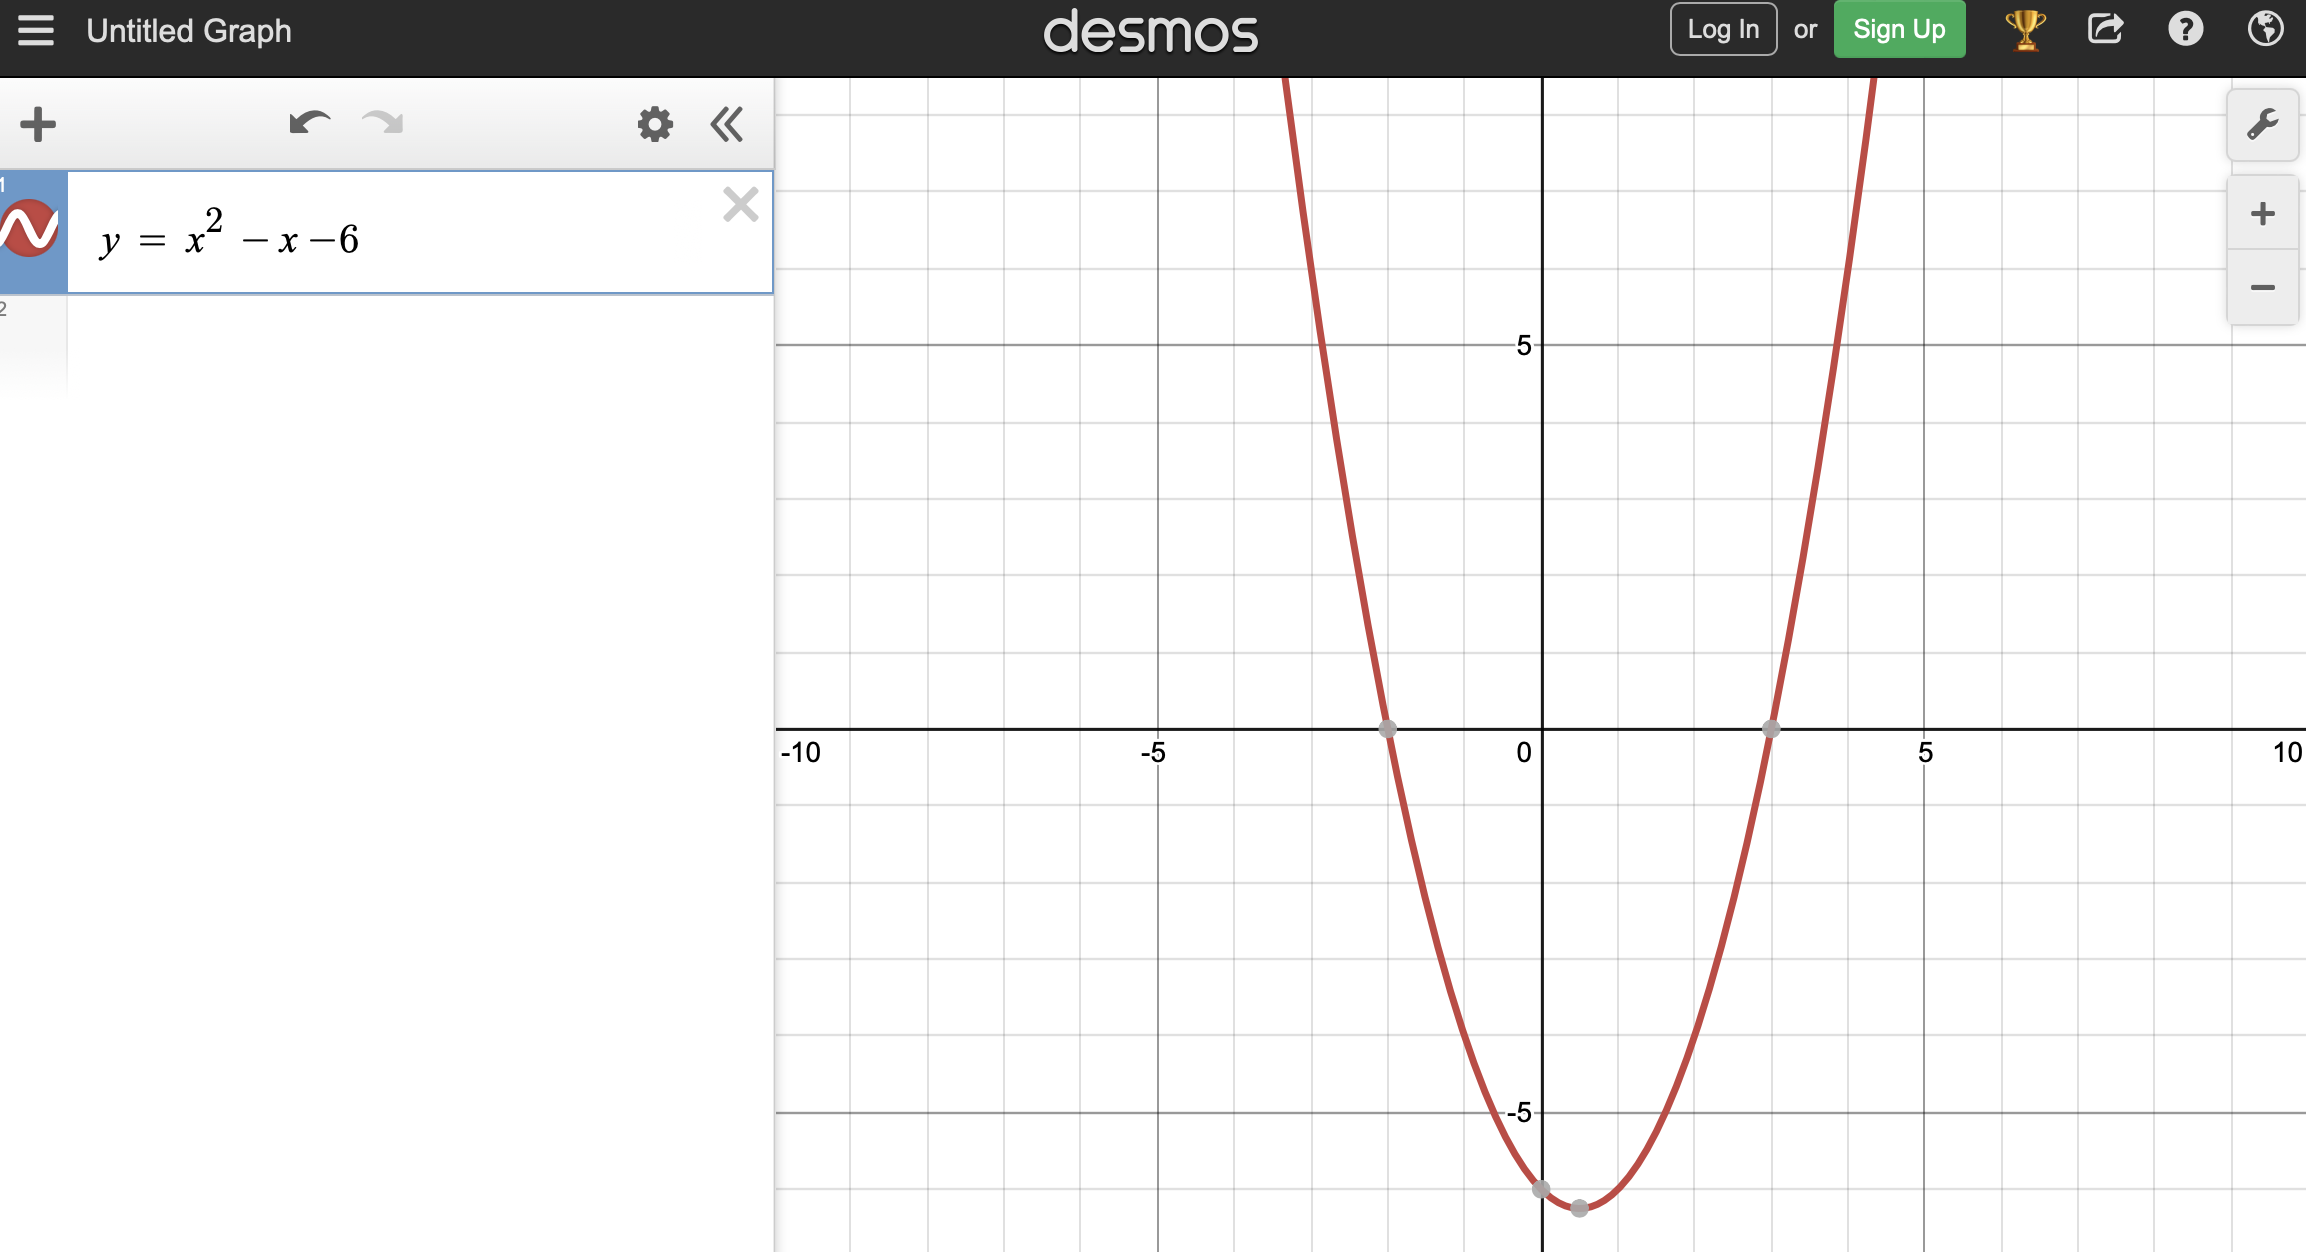
\includegraphics[width=0.85\textwidth]{Desmos.png}

\chapter{Falling Bodies}

Because of gravity, if you throw a hammer straight up in the air, from
the moment it leaves your hand until it hits the ground, it is
accelerating toward the center of the earth at a constant rate.

\emph{Acceleration} can be defined as change in velocity. If the hammer leaves your
hand with a velocity of 12 meters per second upward, one second later
it will be rising, and its velocity will have slowed to 2.2 meters per
second. One second after that, the hammer will be falling at a rate of
7.6 meters per second. Every second the hammer's velocity is changing by
9.8 meters per second, and that change is always toward the center of
the earth. When the hammer is going up, gravity is slowing it down by
9.8 meters per second, each second it is in the air.  When the hammer is coming down,
gravity is speeding it up by 9.8 meters per second.\index{acceleration}
% Connect to vectors

Acceleration due to gravity on earth is a constant negative 9.8 meters per second per second:
\begin{equation*}
a = -9.8   
\end{equation*}
(Why is it negative? We are talking about height, which increases as
you go away from the center of the earth. Acceleration is changing the
velocity in the opposite direction.)

\section{Calculating the Velocity}

Given that the acceleration is constant, it makes sense that the
velocity is a straight line. Assuming once again that the hammer
leaves your hand at 12 meters per second, then the upwards velocity at
time $t$ is given by:
\begin{equation*}
  v = 12 - 9.8t
\end{equation*}

Note that the velocity of the hammer is being given as a function. Here is its graph:

\begin{tikzpicture}
    \begin{axis}[
        xmin=-0.25,xmax=2.75,
        ymin=-13,ymax=13,
        axis x line=middle,
        axis y line=middle,
        axis line style=<->,
        xlabel={$t$},
        ylabel={$v$},
        ]
        \addplot[no marks,sdkblue] expression[domain=0:2.25,samples=100]{x * (-9.8) + 12} node[left] {$12 - 9.8t$}; 
    \end{axis}
\end{tikzpicture}

\begin{Exercise}[title={When is the apex of flight?}, label=vapex]
  Given the hammer's velocity is given by $12 - 9.8t$, at what time (in seconds)
  does it stop rising and begin to fall?
\end{Exercise}
\begin{Answer}[ref=vapex]
  Solve for when the velocity is zero.

  $t = \frac{12}{9.8} = 1.22$ seconds after release.
\end{Answer}

At this point, we need to acknowledge air resistance. Gravity
is not the only force on the hammer; as it travels through the air,
the air tries to slow it down. This force is called \emph{air resistance},
and for a large, fast-moving object (like an airplane) it is GIGANTIC force. For a
dense object (like a hammer) moving at a slow speed (what you generate
with your hand), air resistance doesn't significantly affect acceleration.
% Relate to f=ma

\section{Calculating Position}

If you let go of the hammer when it is 2 meters
above the ground, the height of the hammer is given by:
\begin{equation*}
  p = -\frac{9.8}{2}t^2 + 12t + 2
\end{equation*}

Here is a graph of this function:

\begin{tikzpicture}
    \begin{axis}[
        xmin=-1.2,xmax=3.5,
        ymin=-13,ymax=13,
        axis x line=middle,
        axis y line=middle,
        axis line style=<->,
        xlabel={$t$},
        ylabel={$p$},
      ]
      \addplot[no marks,sdkblue,dashed,<-] expression [domain=-0.7:0,samples=100] {(-4.9)*(x^2) + 12 * x + 2};
      \addplot[no marks,sdkblue] expression [domain=0:2.58,samples=100] {(-4.9)*(x^2) + 12 * x + 2};
      \addplot[no marks,sdkblue,dashed,->] expression [domain=2.58:3,samples=100] {(-4.9)*(x^2) + 12 * x + 2};
    \end{axis}
\end{tikzpicture}


How do we know? \textbf{The change in position between time
  $0$ and any time $t$ is equal to the area under the velocity graph
  between $x = 0$ and $x = t$.}

Let's use the velocity graph to figure out how much the position has
changed in the first second of the hammer's flight. Here's the
velocity graph with the area under the graph for the first second filled
in:

\usepgfplotslibrary{fillbetween}

\begin{tikzpicture}
    \begin{axis}[
        xmin=-0.25,xmax=2.75,
        ymin=-13,ymax=13,
        axis x line=middle,
        axis y line=middle,
        axis line style=<->,
        xlabel={$t$},
        ylabel={$v$},
      ]
      \addplot[no marks,sdkblue, name path=f] expression[domain=0:2.25,samples=100]{x * (-9.8) + 12} node[left] {$12 - 9.8t$};
      \path[name path=xaxis] (axis cs:0,0) -- (axis cs:1,0);
      \addplot[
        thick,
        color=sdkblue,
        fill=sdkblue, 
        fill opacity=0.05
    ]
    fill between[
        of=f and xaxis,
        soft clip={domain=0:1},
    ];
    \addplot[dashed,gray] coordinates {(0,12)(1,12)};
    \addplot[dashed,gray] coordinates {(1,12)(1,0)};
    \end{axis}
\end{tikzpicture}

The blue filled region is the area of the dashed rectangle minus that
empty triangle in its upper left.  The height of the rectangle is
twelve and its width is the amount of time the hammer has been in
flight ($t$). The triangle is $t$ wide and $9.8t$ tall. Thus, the
area of the blue region is given by $12t - \frac{1}{2}9.8 t^2$.

That's the change in position. Where was it originally? 2 meters off
the ground. So the height is given by $p = 2 + 12t - \frac{1}{2}9.8t^2$.
We usually write terms so that the exponent decreases, so:

$$p = - \frac{1}{2}9.8t^2 + 12t + 2$$

Finding the area under the curve like this is called
\textit{integration}. We say ``To find a function that gives the
change in position, we just integrate the velocity function.''  A lot
of the study of calculus is learning to integrate different sorts of
functions.\index{integration}

One important note about integration: Any time the curve drops under
the $x$-axis, the area is considered negative. (Which makes sense,
right? If the velocity is negative, the hammer's position is
decreasing.)


\begin{tikzpicture}
    \begin{axis}[
        xmin=-0.25,xmax=2.75,
        ymin=-13,ymax=13,
        axis x line=middle,
        axis y line=middle,
        axis line style=<->,
        xlabel={$t$},
        ylabel={$v$},
      ]
      \addplot[no marks,sdkblue, name path=f] expression[domain=0:2.25,samples=100]{x * (-9.8) + 12} node[left] {$12 - 9.8t$};
      \path[name path=xaxis] (axis cs:0,0) -- (axis cs:2.25,0);
      \addplot[
        thick,
        color=sdkblue,
        fill=sdkblue, 
        fill opacity=0.05
      ]
      fill between[
        of=f and xaxis,
        soft clip={domain=0:1.2245},
      ];
      \addplot[
        thick,
        color=red,
        fill=red, 
        fill opacity=0.07
      ]
      fill between[
        of=f and xaxis,
        soft clip={domain=1.2245:2.1},
      ];
    \end{axis}
\end{tikzpicture}


\section{Quadratic functions}

Functions of the form $f(x) = a x^2 + b x + c$ are called \newterm{quadratic functions}. 
If $a > 0$, the ends go up.
If $a < 0$, the ends go down.\index{quadratic functions}


\begin{tikzpicture}
  \begin{axis}[
      xmin=-2.2,xmax=1.2,
      ymin=-2,ymax=3,
      axis x line=middle,
      axis y line=middle,
      axis line style=<->,
    ]
    \addplot[no marks,sdkblue] expression [domain=-2:1,samples=100] {(2)*(x^2) + 2 * x - 1};
  \end{axis}
  \node[right] at (1,4) {$2x^2 + 2x - 1$};
\end{tikzpicture}
\hspace{4mm}
\begin{tikzpicture}
  \begin{axis}[
    xmin=-1.5,xmax=1.5,
    ymin=-2,ymax=1.5,
    axis x line=middle,
    axis y line=middle,
    axis line style=<->,
  ]
  \addplot[no marks,sdkblue] expression [domain=-1.5:1.5,samples=100] {(-1.2)*(x^2) + 0.5 * x + 1};
\end{axis}
\node[right] at (0.5,1) {$-1.2 x^2 + 0.5 x + 1$};
\end{tikzpicture}

The graph of a quadratic function is a \newterm{parabola}.

\section{Simulating a falling body in Python}

Now you are going to write some Python code that simulates the flying hammer. First, we are just going to print out the position, speed, and acceleration of the hammer for every 1/100th of a second after it leaves your hand. (Later we will make a graph.)

Create a file called \filename{falling.py} and type this into it:

\begin{Verbatim}
# Acceleration on earth
acceleration = -9.8 # m/s/s

# Size of time step
time_step = 0.01 # seconds

# Initial values
speed = 12  # m/s upward
height = 2  # m above the ground
current_time = 0.0  # seconds after release

# Is the hammer still aloft?
while height > 0.0:

    # Show the values
    print(f"{current_time:.2f} s:")
    print(f"\tacceleration: {acceleration:.2f} m/s/s")
    print(f"\tspeed: {speed:.2f} m/s")
    print(f"\theight: {height:.2f} m")

    # Update height
    height = height + time_step * speed

    # Update speed
    speed = speed + time_step * acceleration

    # Update time
    current_time = current_time + time_step


print(f"Hit the ground: Complete")
\end{Verbatim}

When you run it, you will see something like this:
\begin{Verbatim}
0.00 s:
	acceleration: -9.80 m/s/s
	speed: 12.00 m/s
	height: 2.00 m
0.01 s:
	acceleration: -9.80 m/s/s
	speed: 11.90 m/s
	height: 2.12 m
0.02 s:
	acceleration: -9.80 m/s/s
	speed: 11.80 m/s
	height: 2.24 m
0.03 s:
	acceleration: -9.80 m/s/s
	speed: 11.71 m/s
	height: 2.36 m
...
2.60 s:
	acceleration: -9.80 m/s/s
	speed: -13.48 m/s
	height: 0.20 m
2.61 s:
	acceleration: -9.80 m/s/s
	speed: -13.58 m/s
	height: 0.07 m
Hit the ground: Complete
\end{Verbatim}

Note that the acceleration isn't changing at all, but it is changing
the speed, and the speed is changing the height.

We can see that the hammer in our simulation hits the ground just
after 2.61 seconds.

\subsection{Graphs and Lists}

Now, we are going to graph the acceleration, speed, and height using a
library called matplotlib. However, to make the graphs, we
need to gather all the data into lists.\index{matplotlib}

For example, we will have a list of speeds, and the first three
entries will be 12.0, 11.9, and 11.8.\index{lists, python}

We create an empty list and assign it to a variable like this:
\begin{Verbatim}
x = []
\end{Verbatim}

Then we can add items like this:
\begin{Verbatim}
x.append(3.14)
\end{Verbatim}

To get the first time back, we can ask for the object at index 0.
\begin{Verbatim}
y = x[0]
\end{Verbatim}
Note that the list starts at 0.  So if you have 32 items in the list,
the first item is at index 0. The last item is at index 31.

Duplicate the file \filename{falling.py} and name the new copy \filename{falling\_graph.py}

We are going to make a plot of the height over time. At the start of the program, you will import the
matplotlib library.  At the end of the program, you will create a plot and show it to the user.

In \filename{falling\_graph.py}, add the bold code:

\begin{Verbatim}[commandchars=\\\{\}]
\textbf{import matplotlib.pyplot as plt}

# Acceleration on earth
acceleration = -9.8 # m/s/s

# Size of time step
time_step = 0.01 # seconds

# Initial values
speed = 12  # m/s upward
height = 2  # m above the ground
current_time = 0.0  # seconds after release

\textbf{# Create empty lists}
\textbf{accelerations = []}
\textbf{speeds = []}
\textbf{heights = []}
\textbf{times = []}

# Is the hammer still aloft?
while height > 0.0:

    \textbf{# Add the data to the lists}
    \textbf{times.append(current_time)}
    \textbf{accelerations.append(acceleration)}
    \textbf{speeds.append(speed)}
    \textbf{heights.append(height)}
    
    # Update height
    height = height + time_step * speed

    # Update speed
    speed = speed + time_step * acceleration

    # Update time
    current_time = current_time + time_step

\textbf{# Make a plot}
\textbf{fig, ax = plt.subplots()}
fig.suptitle("Falling Hammer")
\textbf{ax.set_xlabel("Time (s)")}
\textbf{ax.set_ylabel("Height (m)")}
\textbf{ax.plot(times, heights)}
\textbf{plt.show()}
\end{Verbatim}

When you run the program, you should see a graph of the height over time.

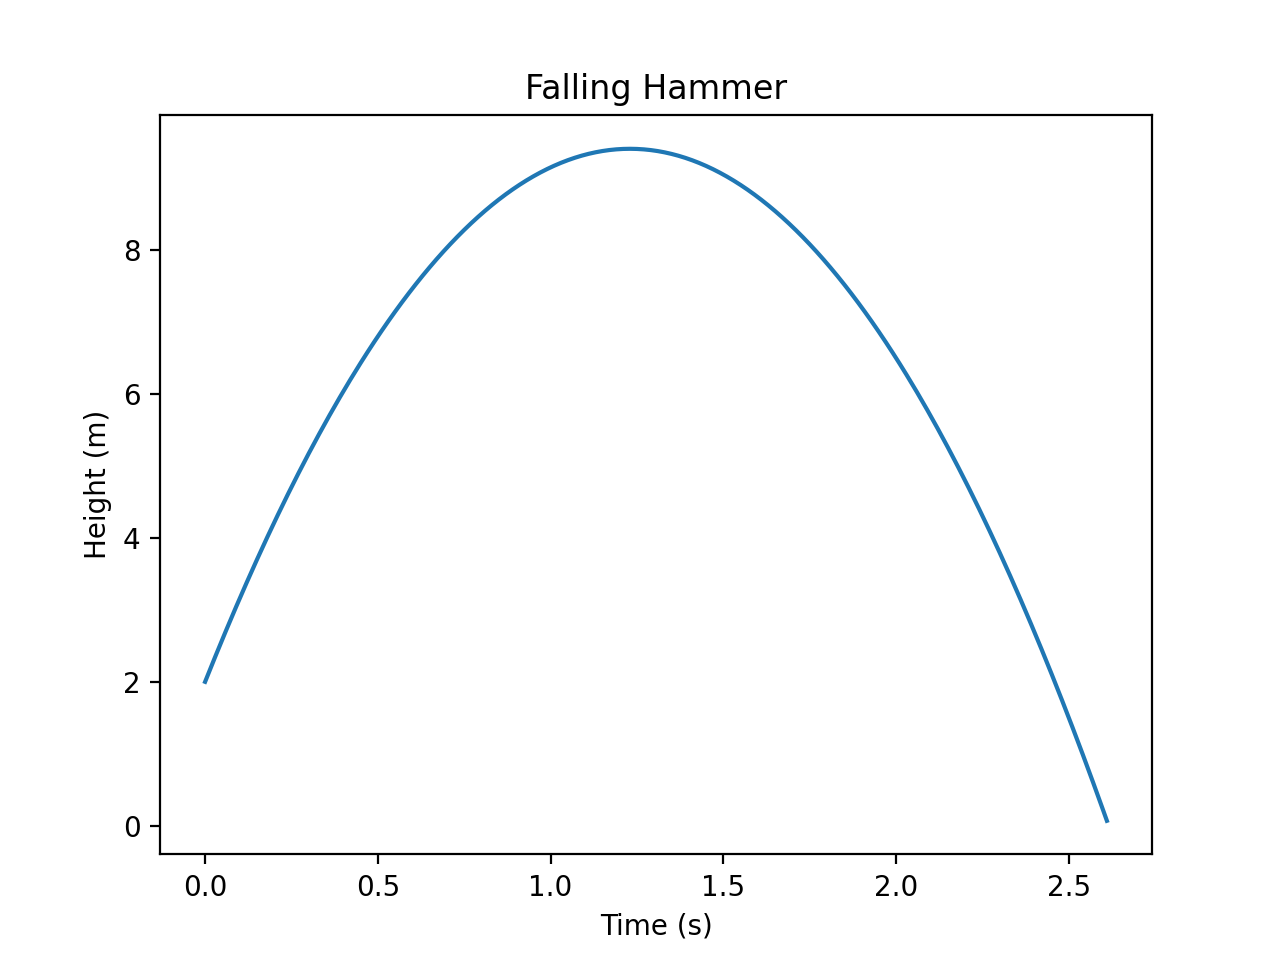
\includegraphics[width=0.7\linewidth]{heightplot.png}

It is more interesting if we can see all three: acceleration, speed, and height. 
So lets make three stacked plots.  Change the plotting code in \filename{falling\_graph.py} to:\index{matplotlib!subplots}

\begin{Verbatim}
# Make a plot with three subplots
fig, ax = plt.subplots(3,1)
fig.suptitle("Falling Hammer")

# The first subplot is acceleration
ax[0].set_ylabel("Acceleration (m/s/s)")
ax[0].plot(times, accelerations)

# Second subplot is speed
ax[1].set_ylabel("Speed (m/s)")
ax[1].plot(times, speeds)

# Third subplot is height
ax[2].set_xlabel("Time (s)")
ax[2].set_ylabel("Height (m)")
ax[2].plot(times, heights)
plt.show()
\end{Verbatim}

Now you will get plots of all three variables:

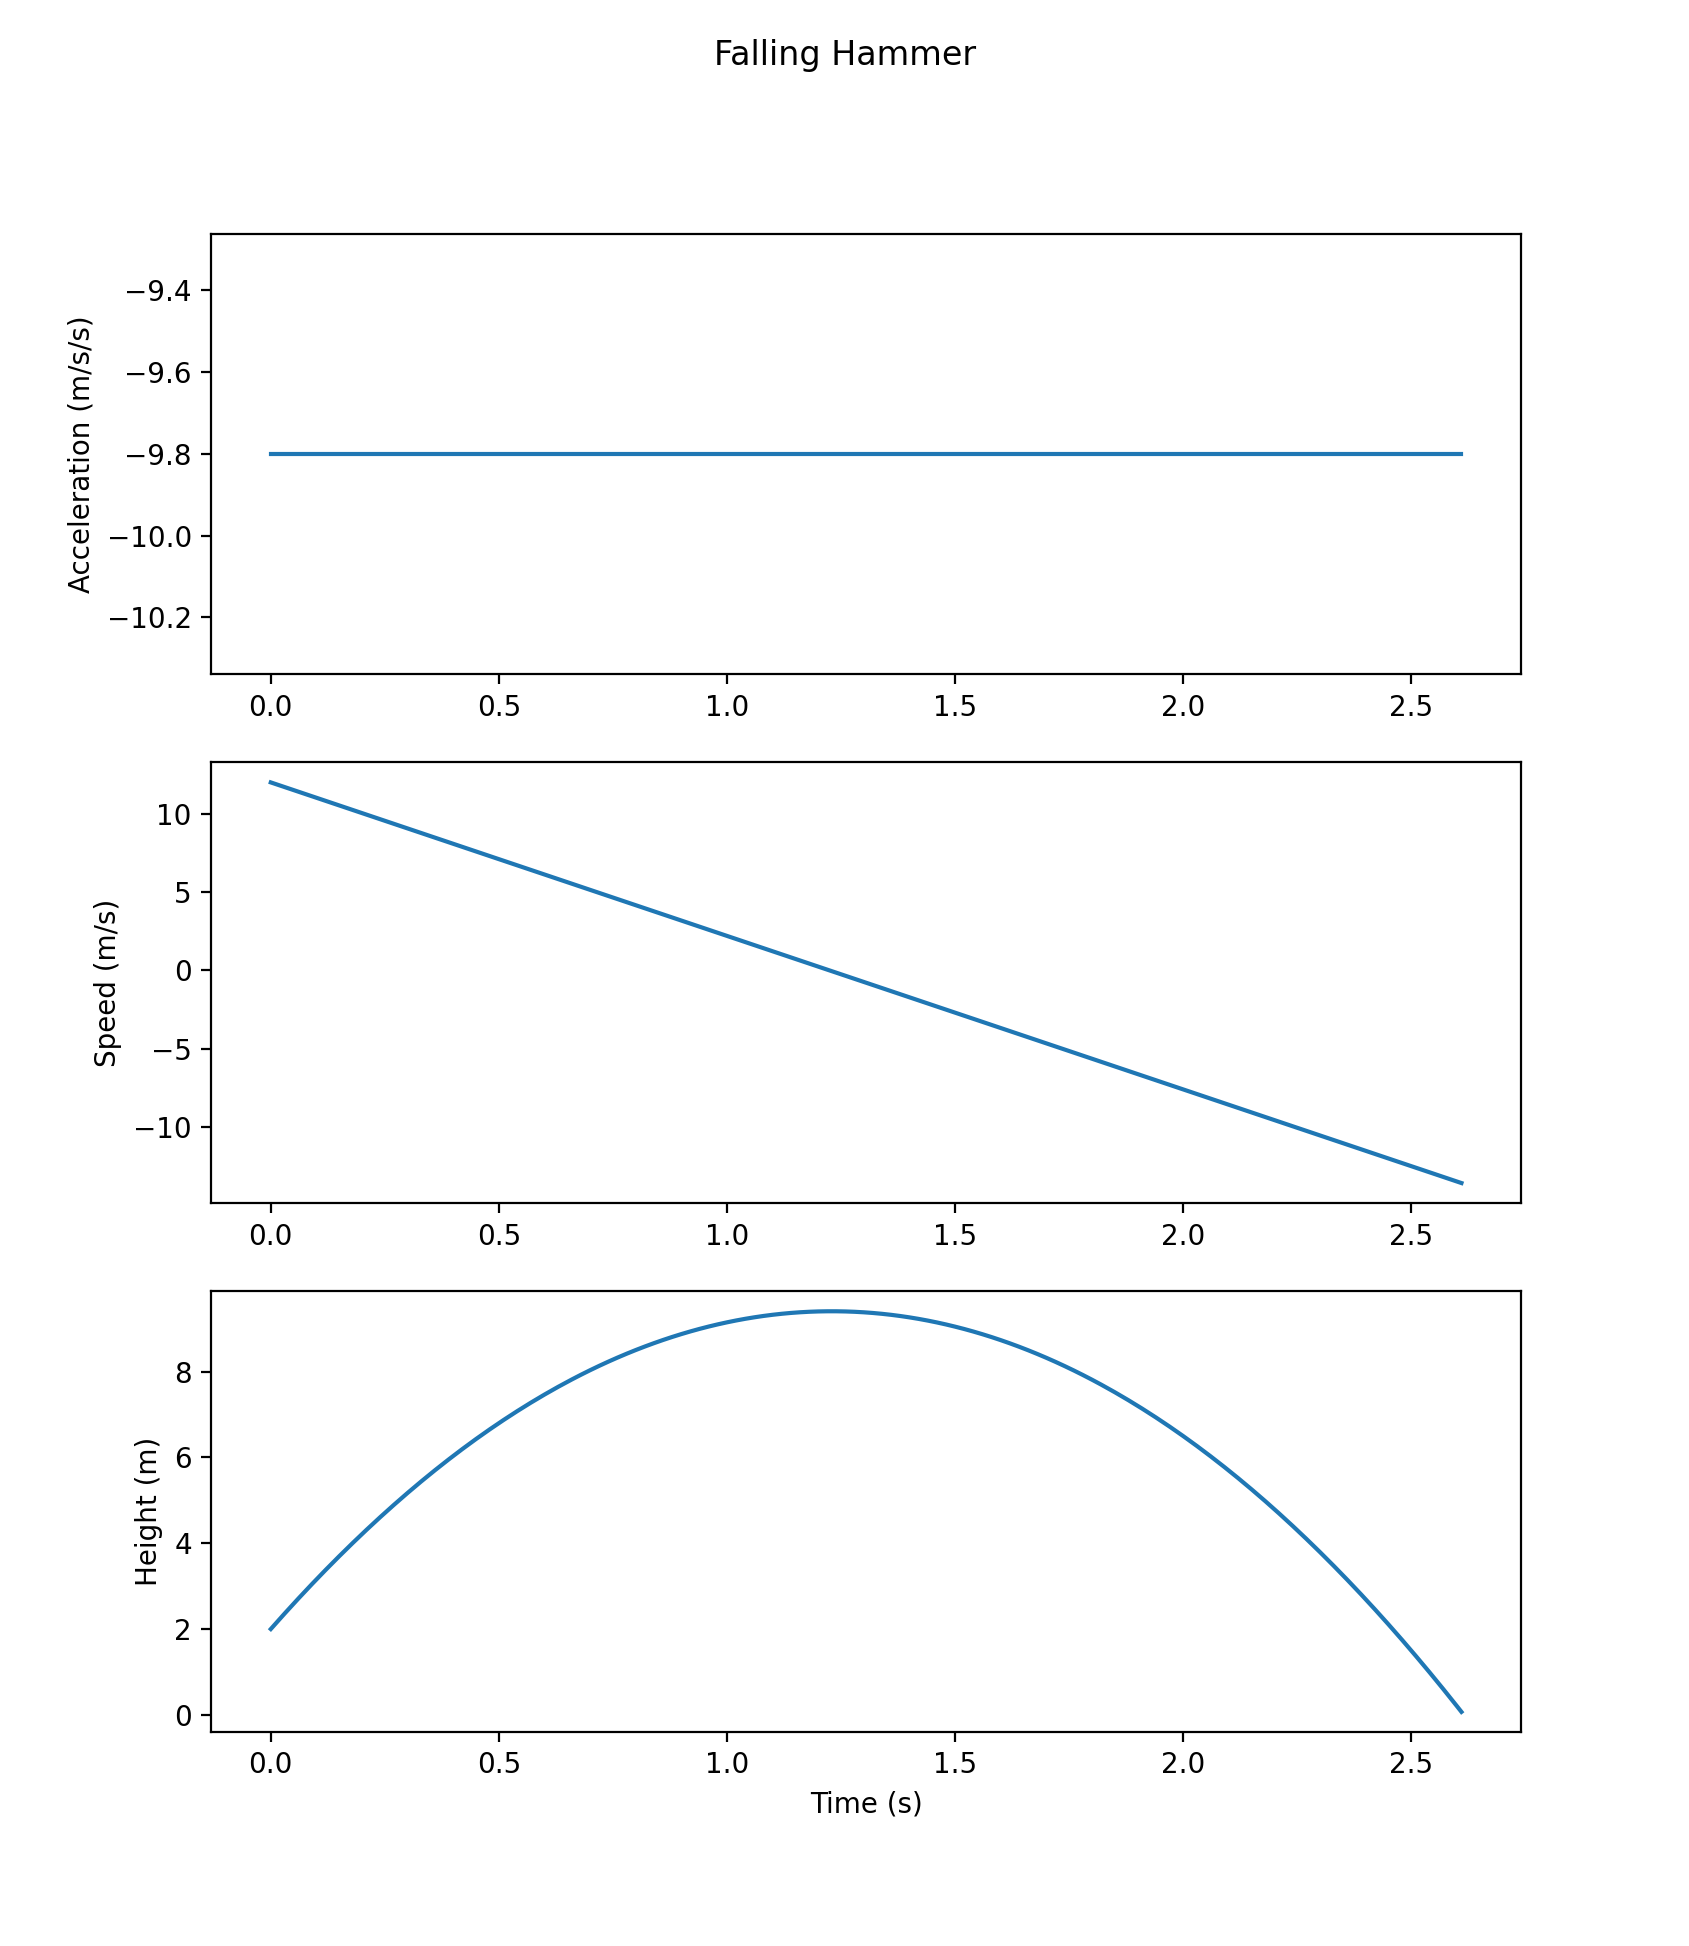
\includegraphics[width=0.8\linewidth]{stackedplot.png}

This is what we expected, right?  The acceleration is a constant negative number.  The speed is a
straight line with a negative slope.  The height is a parabola.

A natural question at this point is ``When exactly will the hammer hit the
ground?''  That is, when does $height = 0$? The values of $t$ where a function is zero are
known as its \textit{roots}. Height is given by a quadratic function. In the next
chapter, you will get the trick for finding the roots of any quadratic
function.

\chapter{Solving Quadratics}

A quadratic function has three terms: $ax^2 + bx + c$. $a$, $b$, and
$c$ are known as the \textit{coefficents}. The coefficients can be any
constant, except that $a$ can never be zero. (If $a$ is zero, it is a linear
function, not a quadratic.)

When you have an equation with a quadratic function on one side and a
zero on the other, you have a quadratic equation. For example:

$$72x^2 - 12x + 1.2 = 0$$

How can you find the values of $x$ that will make this equation true?

You can always reduce a quadratic equation so that the first
coefficient is 1, so that your equation looks like this:

$$x^2 +bx + c = 0$$

For example, if you are asked to solve $4x^2 + 8x - 19 = -2x^2 - 7$
\begin{multline*}
  4x^2 + 8x - 19 = -2x^2 - 7 \\
  6x^2 + 8x -12 = 0 \\
  x^2 + \frac{4}{3}x - 2 = 0
\end{multline*}
Here, $b = \frac{4}{3}$ and $c = -2$.

\begin{mdframed}[style=important]
$x^2 + bx + c = 0$ when
\begin{equation*}
x = -\frac{b}{2} \pm \frac{\sqrt{b^2 - 4c}}{2}  
\end{equation*}
\end{mdframed}

What does this mean?

For any $b$ and $c$, the graph of $x^2 + bx + c$ is a parabola
that goes up on each end. Its low point is at $x = -\frac{b}{2}$.

If there are no real roots ($b^2 - 4c < 0$), that means the
parabola never gets low enough to cross the $x$-axis:

\begin{tikzpicture}
    \begin{axis}[
        xmin=-0.5,xmax=2.75,
        ymin=-1,ymax=5,
        axis x line=middle,
        axis y line=middle,
        axis line style=<->,
        xlabel={$x$},
        ylabel={$y$},
      ]
      \addplot[no marks,sdkblue] expression[domain=-0.25:2.5,samples=100]{x^2 - 2* x + 3} node[above, xshift=-1cm] {$x^2 - 2x + 3$};
      \addplot[dashed,gray] coordinates {(1,-1)(1,3)};
    \end{axis}
\end{tikzpicture}

If there is one real root ($b^2 - 4c = 0$), it means that the parabola just touches the x-axis.

\begin{tikzpicture}
    \begin{axis}[
        xmin=-0.5,xmax=3.75,
        ymin=-0.5,ymax=5,
        axis x line=middle,
        axis y line=middle,
        axis line style=<->,
        xlabel={$x$},
        ylabel={$y$},
      ]
      \addplot[no marks,sdkblue] expression[domain=-0.25:3.5,samples=100]{x^2 - 4*x + 4} node[above, xshift=-1cm] {$x^2 - 4x + 4$};
      \addplot[dashed,gray] coordinates {(2,-0.5)(2,1)};
    \end{axis}
\end{tikzpicture}

If there are two real roots ($b^2 - 4c > 0$), it means that the parabola crosses the x-axis twice as it dips below and then returns:

\begin{tikzpicture}
    \begin{axis}[
        xmin=-0.5,xmax=3.75,
        ymin=-2,ymax=5,
        axis x line=middle,
        axis y line=middle,
        axis line style=<->,
        xlabel={$x$},
        ylabel={$y$},
      ]
      \addplot[no marks,sdkblue] expression[domain=-0.25:3.5,samples=100]{x^2 - 3*x + 1} node[above, xshift=-1cm] {$x^2 - 4x + 4$};
      \addplot[dashed,gray] coordinates {(1.5,-2)(1.5,1)};
    \end{axis}
\end{tikzpicture}

\begin{Exercise}[title={Roots of a Quadratic}, label=solve_quadratic]

  In the last chapter, you found that the function for the height of your flying hammer is:

  $$p = -\frac{1}{2}9.8 t^2 + 12t + 2$$

  At what time will the hammer hit the ground?

  
\end{Exercise}
\begin{Answer}[ref=solve_quadratic]

  For what $t$ is  $-4.9 t^2 + 12t + 2 = 0$?  Start by dividing both sides of the equation by -4.9.

  $$t^2 - 2.45 t - 0.408 = 0$$

  The roots of this are at

  $$x = -\frac{b}{2} \pm \frac{\sqrt{b^2 - 4c}}{2} = -\frac{-2.45}{2} \pm \frac{\sqrt{(-2.45)^2 - 4(-0.408)}}{2} = 1.22 \pm 1.36$$

  We only care about the root after we release the hammer ($t > 0$).

  $1.22 + 1.36 = 2.58$ seconds after releasing the hammer, it will hit the ground.

  
\end{Answer}


\section{The Traditional Quadratic Formula}

I like the approach I just showed you. I find it easier to remember
and easier to prove than the traditional quadratic fomula, but you
should probably know the traditional quadratic formula.

\begin{mdframed}[style=important, frametitle={The Quadratic Formula}]

$ax^2 + bx + c = 0$ when
\begin{equation*}
  x = \frac{-b \pm \sqrt{b^2 - 4ac}}{2a}
\end{equation*}

\end{mdframed}

\chapter{Drag}

The very first computers were created to do calculations of how
artillery would fly when shot at different angles. The calculations
were similar to the ones you just did for the flying
hammer with two important differences:
\begin{itemize}
\item They were interested in two dimensions: the height and the distance across the ground.
\item However, artillery flies a lot faster than a hammer, so they had to worry about drag from the air.
\end{itemize}

\section{Wind resistance}

The first thing they did was put one of the shells in a wind tunnel.
They measured how much force was created when they pushed 1 m/s of
wind over the shell. Let's say it was 0.1 newtons.

One of the interesting things about the drag from the air (often
called \newterm{wind resistance}) is that it increases with the
\emph{square} of the speed. Thus, if the wind pushing on the shell is
3 m/s, instead of 1 m/s, the resistance is $3^2 \times 0.1 = 0.9$
newtons.

(Why? Intuitively, three times as many air molecules are hitting the
shell and each molecule is hitting it three times harder.)

So, if a shell is moving with the velocity vector $v$, the force
vector of the drag points in the exact opposite direction. If $\mu$ is
the force of wind resistance of the shell at 1 m/s, then the magnitude
of the drag vector is $\mu |v|^2$.

\section{Initial velocity and acceleration due to gravity}

Let's say a shell is shot out of a tube at $s$ m/s, and let's say the tube
is tilted $\theta$ radians above level.  Then, the initial velocity
will be given by the vector $[s \cos(\theta), s \sin(\theta)]$

(The velocity of the shell is actually a 3-dimensional vector, but we
are only going to worry about height and horizontal distance; we are
assuming that the operator pointed it in the right direction.)

To figure out the path of the shell, we need to compute its acceleration. We remember that

$$F = m a$$

(Note that $F$ and $a$ are vectors.)  Dividing both sides by $m$ we get:

$$a = \frac{F}{m}$$

So let's figure out the net force on the shell so that we can calculate the acceleration vector.

If the shell has a mass of $b$, the force due to gravity will be in the
downward direction with a magnitude of $9.8 b$ newtons.

To get the net force, we will need to add the force due to gravity
with the force due to wind resistance.

\section{Simulating artillery in Python}

Create a file called \filename{artillery.py}.

\begin{Verbatim}
    import numpy as np
    import matplotlib.pyplot as plt
    
    # Constants
    mass = 45 # kg
    start_speed = 300.0 # m/s
    theta = np.pi/5 # radians (36 degrees above level)
    time_step = 0.01 # s
    wind_resistance = 0.05 # newtons in 1 m/s wind
    force_of_gravity = np.array([0.0, -9.8 * mass]) # newtons
    
    # Initial state
    position = np.array([0.0, 0.0]) # [distance, height] in meters
    velocity = np.array([start_speed * np.cos(theta), start_speed * np.sin(theta)])
    time = 0.0 # seconds
    
    # Lists to gather data
    distances = []
    heights = []
    times = []
    
    # While shell is aloft
    while position[1] >= 0:
        # Record data
        distances.append(position[0])
        heights.append(position[1])
        times.append(time)
    
        # Calculate the next state
        time += time_step
        position += time_step * velocity
    
        # Calculate the net force vector
        force = force_of_gravity - wind_resistance * velocity**2
    
        # Calculate the current acceleration vector
        acceleration = force / mass
    
        # Update the velocity vector   
        velocity += time_step * acceleration
    
    print(f"Hit the ground {position[0]:.2f} meters away at {time:.2f} seconds.")
    
    # Plot the data
    fig, ax = plt.subplots()
    ax.plot(distances, heights)
    ax.set_title("Distance vs. Height")
    ax.set_xlabel("Distance (m)")
    ax.set_ylabel("Height (m)")
    plt.show()        
\end{Verbatim}

When you run it, you should get a message like:
\begin{Verbatim}
Hit the ground 1696.70 meters away at 20.73 seconds.
\end{Verbatim}

You should also see a plot of the shell's path:

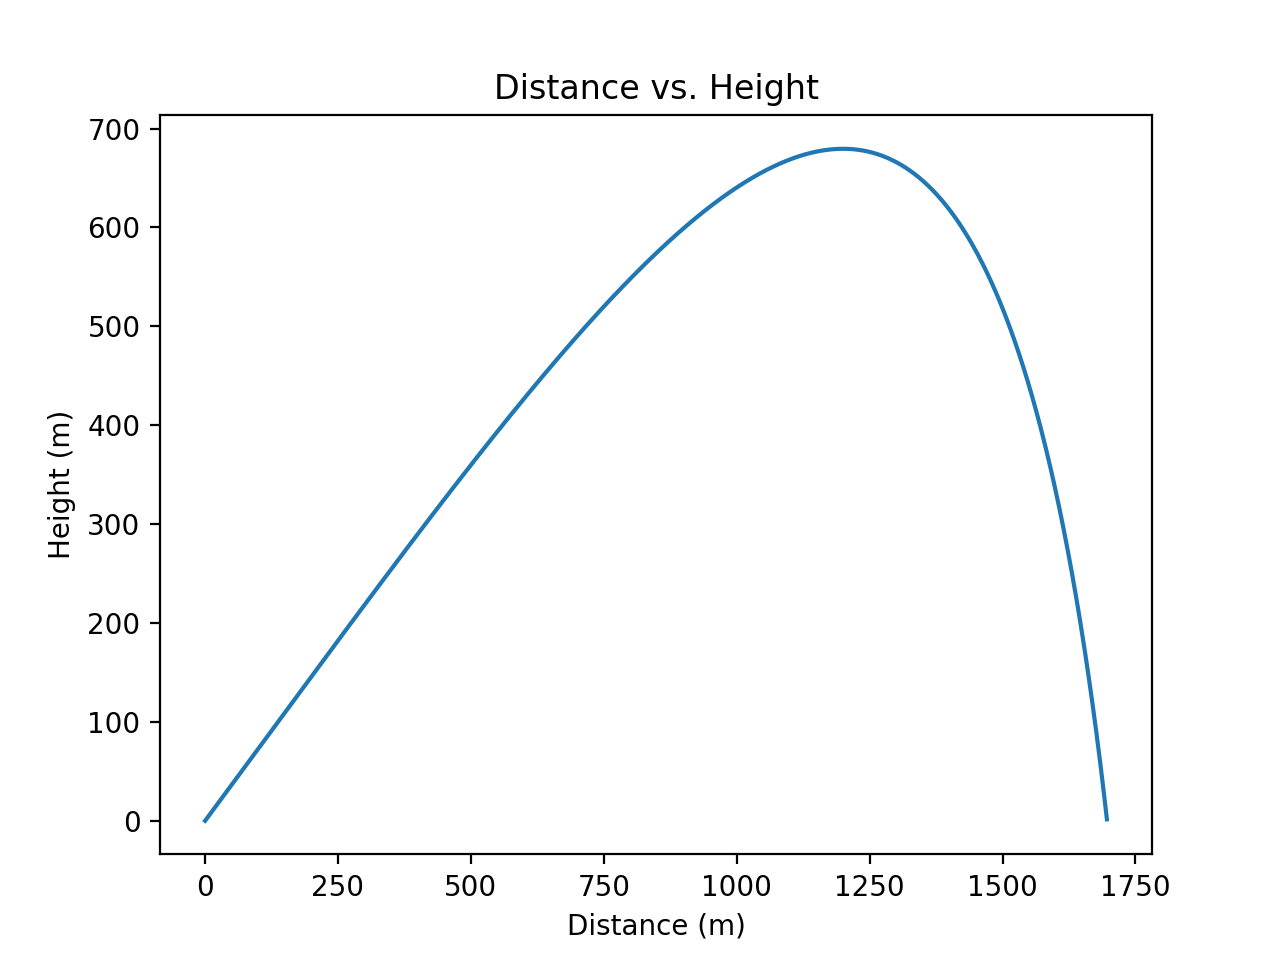
\includegraphics[width=0.8\textwidth]{artillery.png}

\section{Terminal velocity}

If you shot the shell very, very high in the sky, it would keep accelerating 
toward the ground until the force of gravity and the force of the wind resistance were equal.
The speed at which this happens is called the \newterm{terminal velocity}.  The terminal velocity of a
falling human is about 53 m/s.

\begin{Exercise}[title={Terminal velocity}, label=terminal_velocity]
    What is the terminal velocity of shell described in our example?
\end{Exercise}
\begin{Answer}[ref=terminal_velocity]
The force of gravity is $9.8 \times 45 = 441$ newtons.

At any speed $s$, the force of wind resistance is $0.05 \times s^2 = 0.05 s^2$ newtons.

At terminal velocity, $0.05 s^2 = 441$. 

Solving for $s$, we get $s = \sqrt{\frac{441}{0.05}}$

Thus, terminal velocity should be about 94 m/s.

\end{Answer}

\chapter{Vector-valued Functions}

In the last chapter, you calculated the flight of the shell.  For any
time $t$, you could find a vector $[distance, height]$. This can be
thought of as a function $f$ that takes a number and returns a
2-dimensional vector.  We call this a \newterm{vector-valued} function
from $\mathbb{R} \rightarrow \mathbb{R}^2$.
% Define the R symbol

We often make a vector-valued function by defining several real-valued
functions.  For example, if you threw a hammer with an initial upward
speed of 12 m/2 and a horizontal speed of 4 m/s along the $x$ axis from
the point $(1, 6, 2)$, its position at time $t$ (during its flight) would be given by:
% Format 12/ m2
$$f(t) = [4t + 1, 6, -4.8t^2 + 12t + 2]$$

That is, $x$ is increasing with $t$, $y$ is constant, and $z$ is a parabola.

\tdplotsetmaincoords{80}{20} 
\begin{tikzpicture} [scale=0.5, tdplot_main_coords, axis/.style={->,sdkblue}, 
vector/.style={-stealth,black,very thick}, 
vector guide/.style={dashed,sdkblue}]

%standard tikz coordinate definition using x, y, z coords
\coordinate (O) at (0,0,0);

%draw axes
\draw[axis] (0,0,0) -- (12,0,0) node[anchor=north east]{$x$};
\draw[axis] (0,0,0) -- (0,7,0) node[above]{$y$};
\draw[axis] (0,0,0) -- (0,0,10) node[anchor=south]{$z$};

\draw[thick,draw=black,
      domain=0:2.60563,samples=300,variable=\t] 
      plot ({4*\t + 1},6, {-4.9*\t^2 + 12*\t + 2});
\draw[dashed,draw=sdkblue] (1, 6, 0) -- (11.42252, 6, 0);
\draw[dashed,draw=sdkblue] (11.42252, 0, 0) -- (11.42252, 6, 0);
\draw[dashed,draw=sdkblue] (1, 6, 0) -- (1, 6, 2);
\draw[dashed,draw=sdkblue] (1, 6, 0) -- (1, 6, 2);
\draw[dashed,draw=sdkblue] (1, 6, 0) -- (1, 0, 0);

\filldraw[black] (1,6,2) circle(4pt) node [left]{$f(0) = [1,6,2]$};
\filldraw[black] (5,6,9.1) circle(4pt) node [above]{$f(1) = [5, 6, 9.1]$};
\draw[dashed,draw=sdkblue] (5, 6, 0) -- (5, 6, 9.1);
\filldraw[black] (9,6,6.4) circle(4pt) node [right]{$f(2) = [9, 6, 6.4]$};
\draw[dashed,draw=sdkblue] (9, 6, 0) -- (9, 6, 6.4);
\filldraw[black] (11.42252,6,0) circle(4pt) node [right] {$f(2.6) = [11.4, 6, 0]$};
\end{tikzpicture}

\section{Finding the velocity vector}


Now that we have its position vector, we can differentiate each
component separately to get its velocity as a vector-valued function:

$$f'(t) = [4, 0, -9.8t + 12]$$

That is, the velocity is constant along the $x$-axis, zero along the
$y$-axis, and decreasing with time along the $z$ axis.

\tdplotsetmaincoords{80}{20} 
\begin{tikzpicture} [scale=0.5, tdplot_main_coords, axis/.style={->,sdkblue}, 
vector/.style={-stealth,black,very thick}, 
vector guide/.style={dashed,sdkblue}]

%standard tikz coordinate definition using x, y, z coords
\coordinate (O) at (0,0,0);

%draw axes
\draw[axis] (0,0,0) -- (14,0,0) node[anchor=north east]{$x$};
\draw[axis] (0,0,0) -- (0,7,0) node[above]{$y$};
\draw[axis] (0,0,0) -- (0,0,10) node[anchor=south]{$z$};

\draw[thick,dashed,draw=black,
      domain=0:2.60563,samples=300,variable=\t] 
      plot ({4*\t + 1},6, {-4.9*\t^2 + 12*\t + 2});

\filldraw[black] (1,6,2) circle(4pt);
\draw[->, thick, draw=black] (1,6,2) -- (5, 6, 14) node [right] {$f'(0) = [4,0,12]$};
\draw[dashed, draw=sdkblue] (1,6,2) -- (5,6,2) -- (5,6,14);
\filldraw[black] (5,6,9.1) circle(4pt);
\draw[->, thick, draw=black] (5,6,9.1) -- (9, 6, 11.3) node [right] {$f'(1) = [4,0,2.2]$};
\draw[dashed, draw=sdkblue] (6,6,9.1) -- (9,6,9.1) -- (9,6,11.3);
\filldraw[black] (9,6,6.4) circle(4pt);
\draw[->, thick, draw=black] (9,6,6.4) -- (13, 6, -1.2) node [right] {$f'(2) = [4,0,-7.6]$};
\filldraw[black] (11.42252,6,0) circle(4pt);
\draw[dashed, draw=sdkblue] (9,6,6.4) -- (13,6,6.4) -- (13,6,-1.2);
\end{tikzpicture}


\section{Finding the acceleration vector}


Now that we have its velocity, we can get its acceleration as a vector-valued function:

$$f''(t) = [0, 0, -9.8]$$

There is no acceleration along the $x$ or $y$ axes. It is accelerating
down at a constant $9.8 m/s^2$.

\tdplotsetmaincoords{80}{20} 
\begin{tikzpicture} [scale=0.5, tdplot_main_coords, axis/.style={->,sdkblue}, 
vector/.style={-stealth,black,very thick}, 
vector guide/.style={dashed,sdkblue}]

%standard tikz coordinate definition using x, y, z coords
\coordinate (O) at (0,0,0);

%draw axes
\draw[axis] (0,0,0) -- (14,0,0) node[anchor=north east]{$x$};
\draw[axis] (0,0,0) -- (0,7,0) node[above]{$y$};
\draw[axis] (0,0,0) -- (0,0,10) node[anchor=south]{$z$};

\draw[thick,dashed,draw=black,
      domain=0:2.60563,samples=300,variable=\t] 
      plot ({4*\t + 1},6, {-4.9*\t^2 + 12*\t + 2});

\filldraw[black] (1,6,2) circle(4pt);
\draw[->, thick, draw=black] (1,6,2) -- (1, 6, -7.8) node [right] {$f''(0) = [0,0,-9.8]$};
\filldraw[black] (5,6,9.1) circle(4pt);
\draw[->, thick, draw=black] (5,6,9.1) -- (5, 6, -0.7) node [below] {$f''(1) = [0,0,-9.8]$};
\filldraw[black] (9,6,6.4) circle(4pt);
\draw[->, thick, draw=black] (9,6,6.4) -- (9, 6, -3.4) node [right] {$f''(2) = [0,0,-9.8]$};
\filldraw[black] (11.42252,6,0) circle(4pt);
\end{tikzpicture}


\graphicspath{{../../Modules/Exponents/}}
\chapter{Introduction to Spreadsheets}

For many real-world problems, spreadsheets are the perfect
tool. In this chapter, you will be introduced to how to use a
spreadsheet. There are numerous spreadsheet programs: Google Sheets,
Microsoft Excel, Apple Numbers, OpenOffice Calc, etc.  All of them are
very similar. This instruction will use Google Sheets, but if you are using one
of the others, you should be able to follow along.

The first spreadsheet program (VisiCalc) was introduced in 1979 as a
tool for finance people to play ``what if'' games.  For example, a
company might make a spreadsheet that told them how much more profit
they would make if they changed from using an expensive metal to using
a cheaper alloy.\index{Spreadsheet}

In honor of its history, let's start by studying a business question:
I have a friend who dreams of quitting her job to become a cooper. (A
cooper makes barrels that are used for aging wine and whiskey.)  She
says:
\begin{itemize}
\item It costs \$45 dollars in materials to build one barrel.
\item A barrel sells for \$100 dollars.
\item The workshop/warehouse she wants to rent costs \$2000 per month.
\item Taxes take 20\% of her profits.
\item She needs to make \$4000 monthly after taxes.
\end{itemize}

She has asked you, ``How many barrels do I need to make each month?''

\section{Solving It Symbolically}

Many problems can be solved two ways: symbolically or
numerically.\index{symbolic vs. numeric solutions} To solve this
problem symbolically, you would write out the facts as equations or
inequalities and then do symbol manipulations until you ended up with
an answer. In this case, you would let $b$ be the number of barrels
and create the following inequality:

$$(1.0 - 0.2)\left(b(100 - 45) - 2000\right) \geq 4000$$

You would simplify it:

$$(0.8)\left(55 b - 2000\right) \geq 4000$$

And simplify it more:

$$44b - 1600 \geq 4000$$

If that is true, then:

$$44b \geq 5600$$

And if that is true, then:

$$b \geq \frac{1400}{11}$$

$1400/11$ is about 127.27, so she needs to make and sell 128 barrels
each month.

That is a perfect answer, and we didn't need a spreadsheet at all. Two things:
\begin{itemize}
\item As problems get larger and more realistic, it gets much more difficult to solve them symbolically.
\item As soon as you say ``Yes, you need to make and sell 128 barrels
  each month.'' Your friend will ask ``What if I make and sell 200
  barrels? How much money will I make then?''
\end{itemize}

So we use a spreadsheets to solve the problem numerically.

\section{Solving It Numerically (with a spreadsheet)}


Let's get back to our example. Put labels in the A column:
\begin{itemize}
\item{Barrels produced (per month)}
\item{Materials cost (per barrel)}
\item{Sale price (per barrel)}
\item{Pre-tax earnings (per month)}
\item{Taxes (per month)}
\item{Take home pay (per month)}
\end{itemize}

Format them any way you like. It should look something like this:

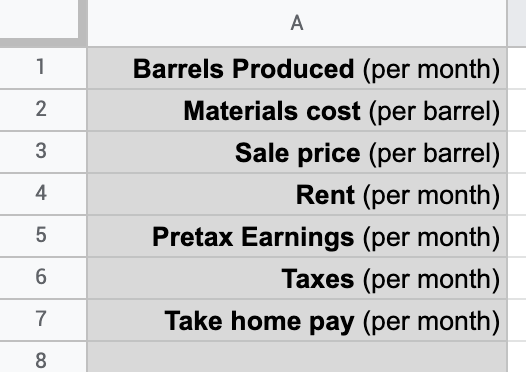
\includegraphics[width=0.4\textwidth]{BarrelLabels.png}

In the B column, the first four cells are values (not formulas):
\begin{itemize}
\item{115 formatted as a number with no decimal point}
\item{45 formatted as currency}
\item{100 formatted as currency}
\item{2000 formatted as currency}
\end{itemize}

It should look something like this:

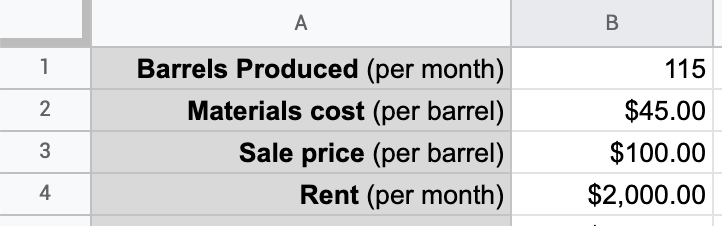
\includegraphics[width=0.5\textwidth]{BarrelValues.png}

The next three cells in the B column will have formulas:
\begin{itemize}
\item{B1 * (B3 - B2) - B4}
\item{0.2 * B5}
\item{B5 - B6}
\end{itemize}

It should look something like this:

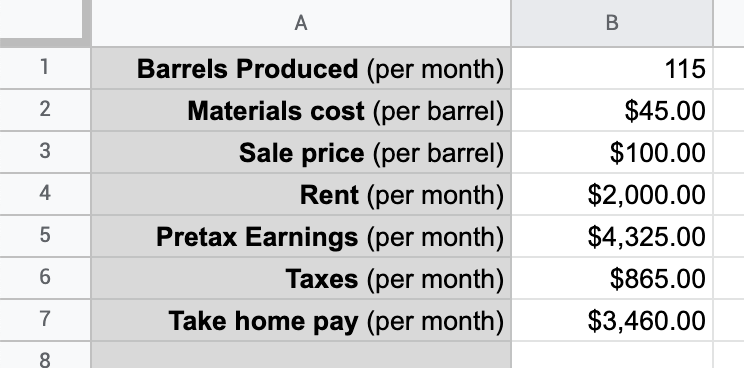
\includegraphics[width=0.5\textwidth]{BarrelFormulas.png}

Now you can share this spreadsheet with your friend and she can put
different values into the cells for what-if games.  Like ``If I can
get my materials cost down to \$42 per barrel, what happens to my take
home pay?''

Sometimes it is nice to show a range of values for a variable or two.
In this case, it might be nice to show your friend what the numbers
look like if she produces 115, 120, 125, 130, 135, or 140 barrels per
month.

We have one column, and now we need six. How do we duplicate cells?
\begin{enumerate}
\item Click B1 to select it and then shift-click on B7 to select all seven cells.
\item Copy them. (There is probably a menu item for this.)
\item Click C1 to select it
\item Paste them.
\end{enumerate}

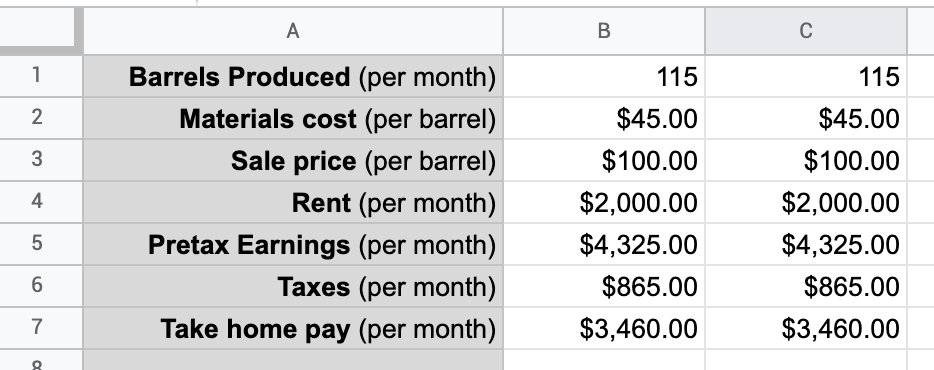
\includegraphics[width=0.5\textwidth]{BarrelCopyPaste.png}

We want the first cell in the new column to be 120. You could just
type in 120, but let's do something more clever.  Put a formula into that
cell: = B1 + 5.  Now the cell should show 120.

Why did we put in a formula? When we duplicate this column, this cell
will always have 5 more barrels than the cell to its left.

Now let's duplicate the second column a few times. The easy way to do
this is to select the cells as you did before and drag the lower-right
corner to the right until column G is in the selection. When you end
the drag, the copies will appear:

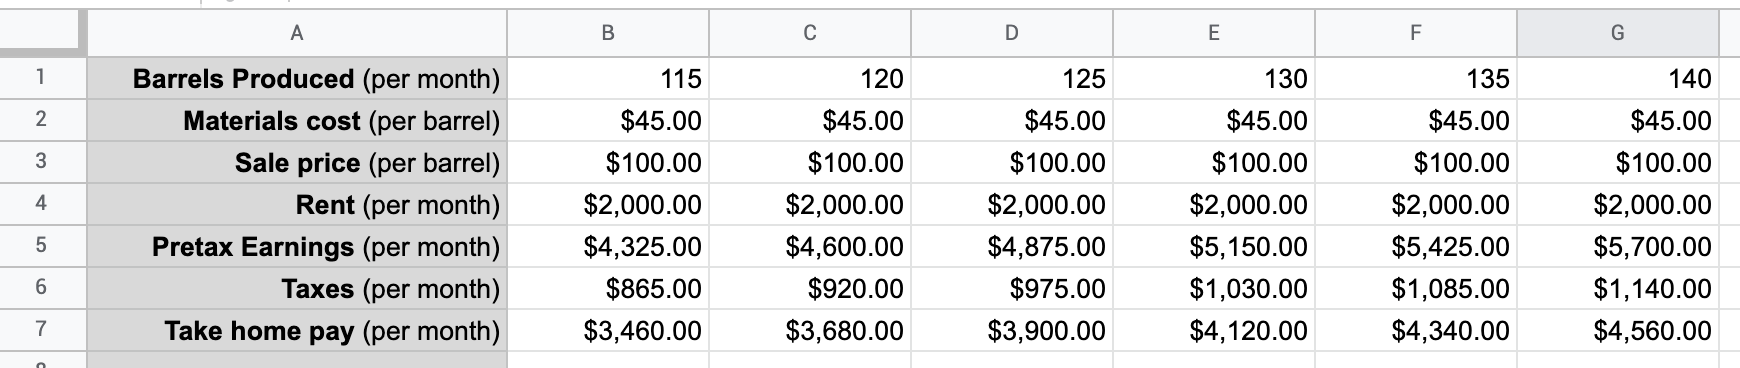
\includegraphics[width=0.8\textwidth]{BarrelDragPaste.png}

Nice, right? Now your friend can easily see how many barrels
correspond to how much take-home pay. Do you know what would be really helpful? A graph.

\section{Graphing}

Graphing is a little different on every different platform.  Here is what you want the graph to look like.

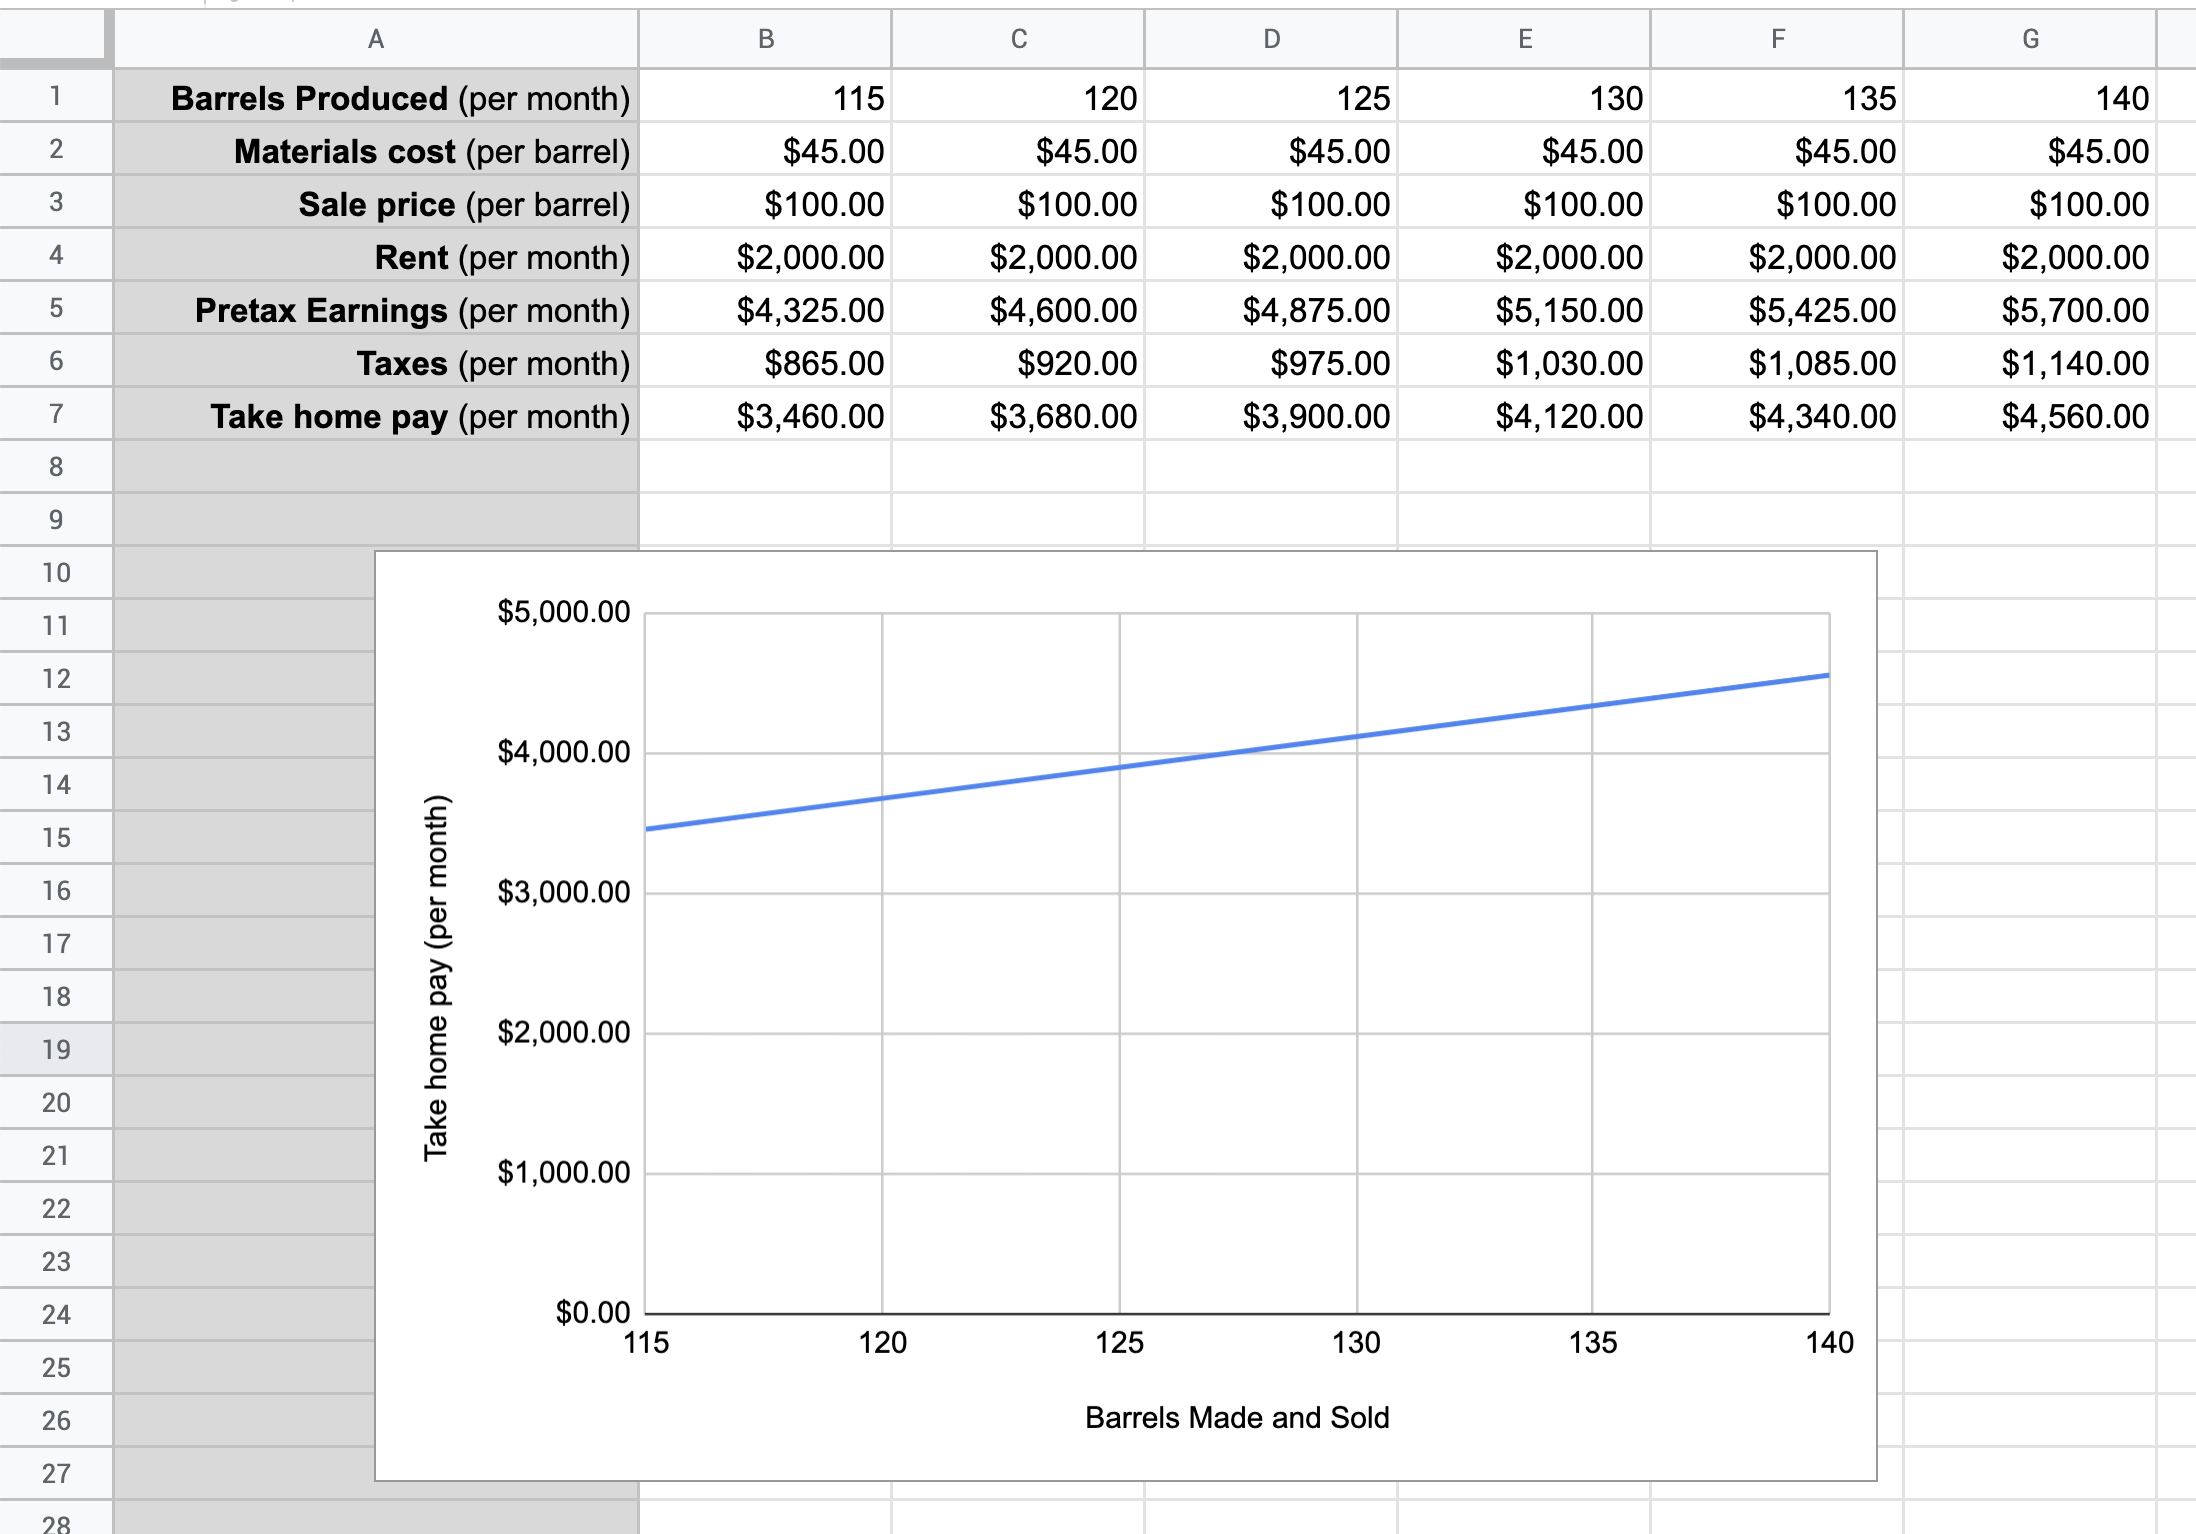
\includegraphics[width=0.8\textwidth]{BarrelGraph.png}

On Google Sheets:\index{spreadsheet!graphs}

\begin{enumerate}
\item Select cells B7 through G7. 
\item Choose the menu item Insert -> Chart.
\item Choose the chart type (Line)
\item Add the X-axis to be B1 through G1.
\item Under the Customize tab, Set the label for the X-axis to be ``Barrels Made and Sold''.
\item Delete the chart title (which is the same as the Y-axis label).
\end{enumerate}

\section{Other Things You Should Know About Spreadsheets}

Your spreadsheet document can have several ``Sheets''.  Each has its
own grid of cells.  The sheet has a name; usually, you call it
something like ``Salaries''.  When you need to use a value from the
``Salaries'' sheet in another sheet, you can specify ``Salaries!A2''
-- that is, cell A2 on sheet ``Salaries''.  To flip between the sheets
there is usually a tab for each at the bottom of the document.

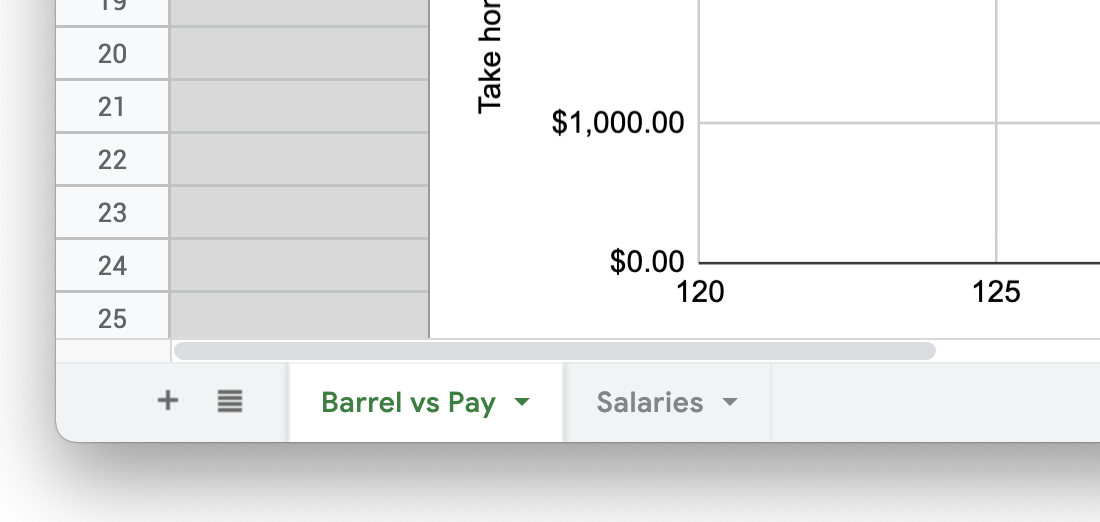
\includegraphics[width=0.5\textwidth]{Sheets.png}

By default, the cell references are relative.  That is when you write
a formula in cell H5 that references the value in cell G4, the cell
remembers ``The cell that is one up and one to the left of me.''
Thus, if you copy that formula into B9, now that formula reads the
value from A8.

If you want an absolute reference, you use \$.  If H5 references
\$G\$4, G4 will be used no matter where on the sheet the formula is
copied to.

You can use the \$ on the row or column.  In \$A4, the column is
absolute and the row is relative.  In A\$4, the row is absolute and
the column is relative.

\section{Challenge: Make a spreadsheet}

You have a company that bids on painting jobs. Make a
spreadsheet to help you do bids. Here are the parameters:
\begin{itemize}
\item The client will tell you how many square meters of wall needs to be painted.
\item Paint costs \$0.02 per square meter of wall
\item On average, a square meter of wall takes 0.02 hours to paint.
\item You can hire painters at \$15 per hour.
\item You add 20\% to your estimated costs for a margin of error and profit.
\end{itemize}

Make a spreadsheet such that when you type in the square meters to be
painted, the spreadsheet tells you how much you will spend on paint
and labor.  It also tells you what your bid should be.

\chapter{Compound Interest}

When you loan money to someone, you typically charge them some sort of
interest. The most common loan of this sort is what the bank calls a
``savings account''.  Any money you put in the account is loaned to
the bank. The bank then lends it to someone else, who pays interest to
the bank. And the bank gives some of that interest to you.

However, what if you leave the interest in your account? And you start
making \textit{interest on the interest}? This is known as
\textit{compound interest}.\index{compound interest}

\section{An example with annual interest payments}

Lets say that you put \$1000 in a savings account that pays 6\%
interest every year. How much money would you have after 12 years?
Let's make a spreadsheet.

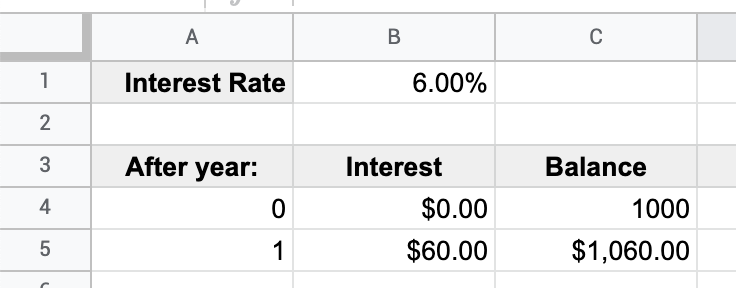
\includegraphics[width=0.4\textwidth]{StartInterest.png}

Create a new spreadsheet and edit the cells to look like this.  All
the cells in row 1 - 4 are just values: just type in what you
see.

The fifth row is all formulas:

\begin{tabular}{c | c | c}
  After year & Interest & Balance \\
  \hline 
  = A4 + 1 & = B\$1 * C4 & = C4 + B5 \\
\end{tabular}

The interest rate field should be formatted as a percentage. One thing
to know when dealing with percentages in the spreadsheet: if the field
says ``600\%'', its value is 6. 

The cells in the Interest and Balance column should be formatted as currency.

You are about to make a bunch of copies of the cells in the fifth row,
so make sure they look right.

Click on A5 and shift click on C5 to select all three cells. Drag the
lower-right corner down to fill the rows 6 - 15.

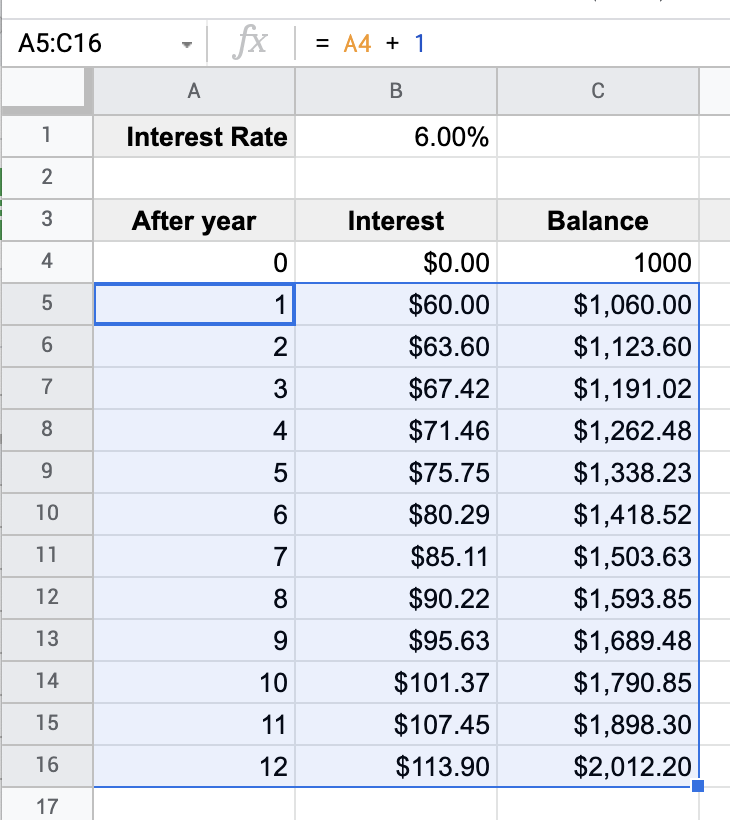
\includegraphics[width=0.5\textwidth]{CopiedCellsInterest.png}

Look at the numbers.  The first interest payment is \$60, but the last
is \$113.90. Your balance has more than doubled!

\section{Exponential Growth}

We figured this out numerically by repeatedly multiplying the balance
by the interest rate.  What if you wanted to know what the balance
would be $n$ years after investing $P_0$ dollars with an annual interest
rate of $r$? (Note that $r$ in our example would be 0.06, not 6.0.)

Each year, the balance is multiplied by $1 + r$, so after one year,
$P_0$ would become $P_0 \times (1 + r)$.  The next year you would multiply
this number by $(1 + r)$ again: $P_0 \times (1 + r) \times (1 + r)$. The
next year? $P_0 \times (1 + r) \times (1 + r) \times (1 + r)$ See the
pattern? If we define $P_n$ be this balance after $n$ years, then

$$P_n = P_0 (1+r)^n$$

Because $n$ is an exponent, we call this \textit{exponential growth}.
And there are few things as terrifying to a scientist as
the phrase ``The population is undergoing exponential growth''.\index{exponential growth}

\section{Sensitivity to interest rate}

For most people, the first surprising thing about compound interest is
how quickly your money grows after a few years.  The second thing that
is surprising is how much difference a small change in the percentage
rate makes.

Lets add another set of columns that shows what happens to your money
if you convince the bank to pay you 8\% instead of 6\%.

Copy everything from columns B and C:

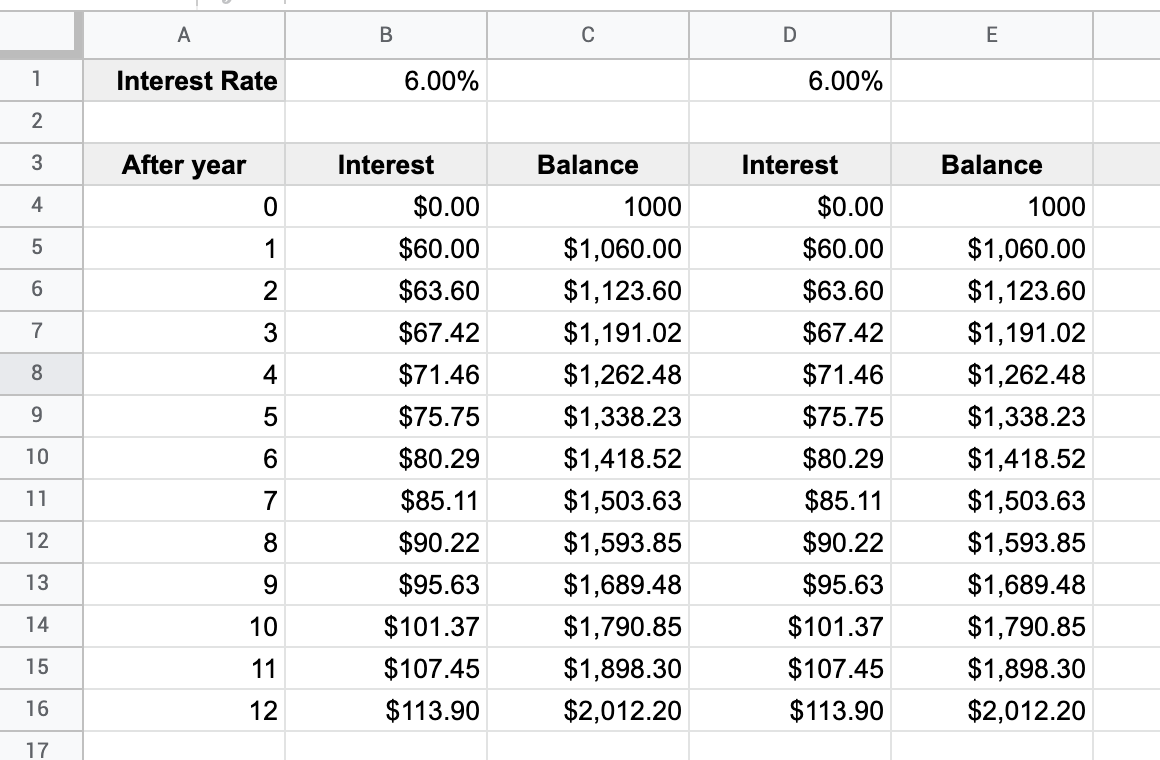
\includegraphics[width=0.6\textwidth]{CopyForSecondInterest.png}

Now edit the second interest rate to be 8\%:

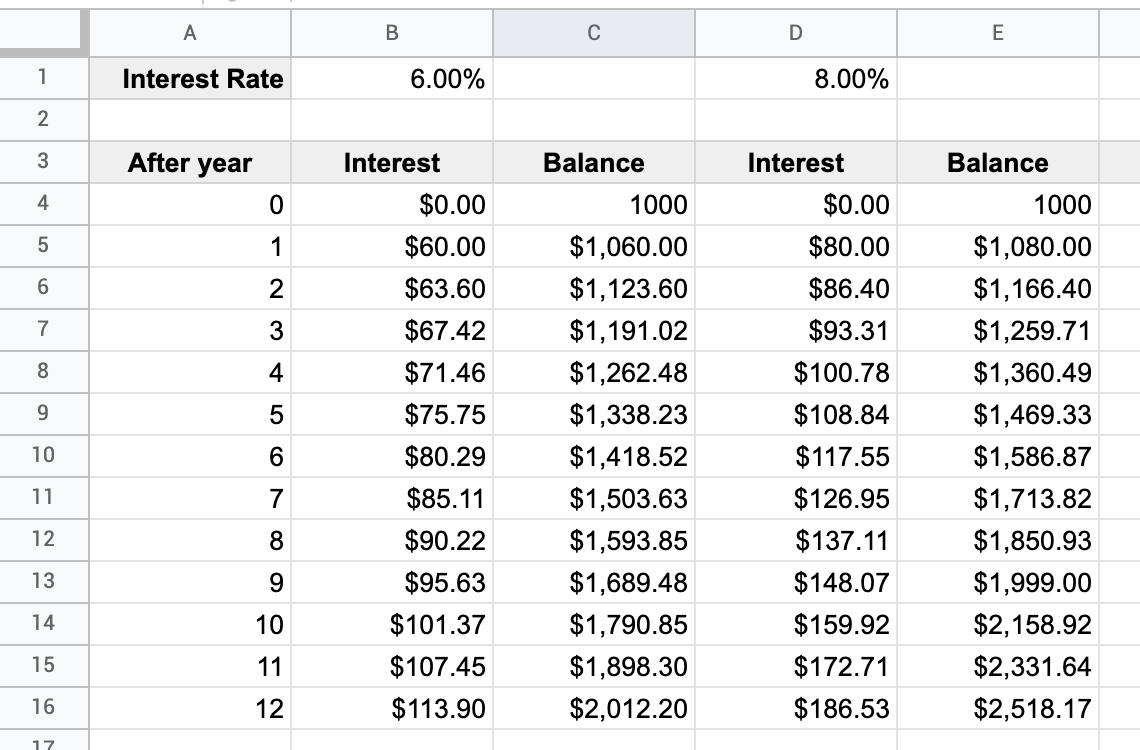
\includegraphics[width=0.6\textwidth]{AtBiggerInterestRate.png}


\chapter{Introduction to Data Visualization}

It is difficult for the human mind to look at a list of numbers and
identify the patterns in them, so we often make pictures with the
numbers. These pictures are called \textit{graphs},
\textit{charts}, or \textit{plots}. Often the right picture can make
the meaning in the data obvious. \textit{Data visualization} is the
process of making pictures from numbers.

\section{Common Types of Data Visualizations}

Depending on the type of data and what you are trying to demonstrate
about it, you will use different types of data visualizations.  How
many types of data visualizations are there? Hundreds, but we will
concentrate on just four: The bar chart, the line graph, the pie
chart, and the scatter plot.

\subsection{Bar Chart}

Here is an example of a bar chart.\index{bar chart}

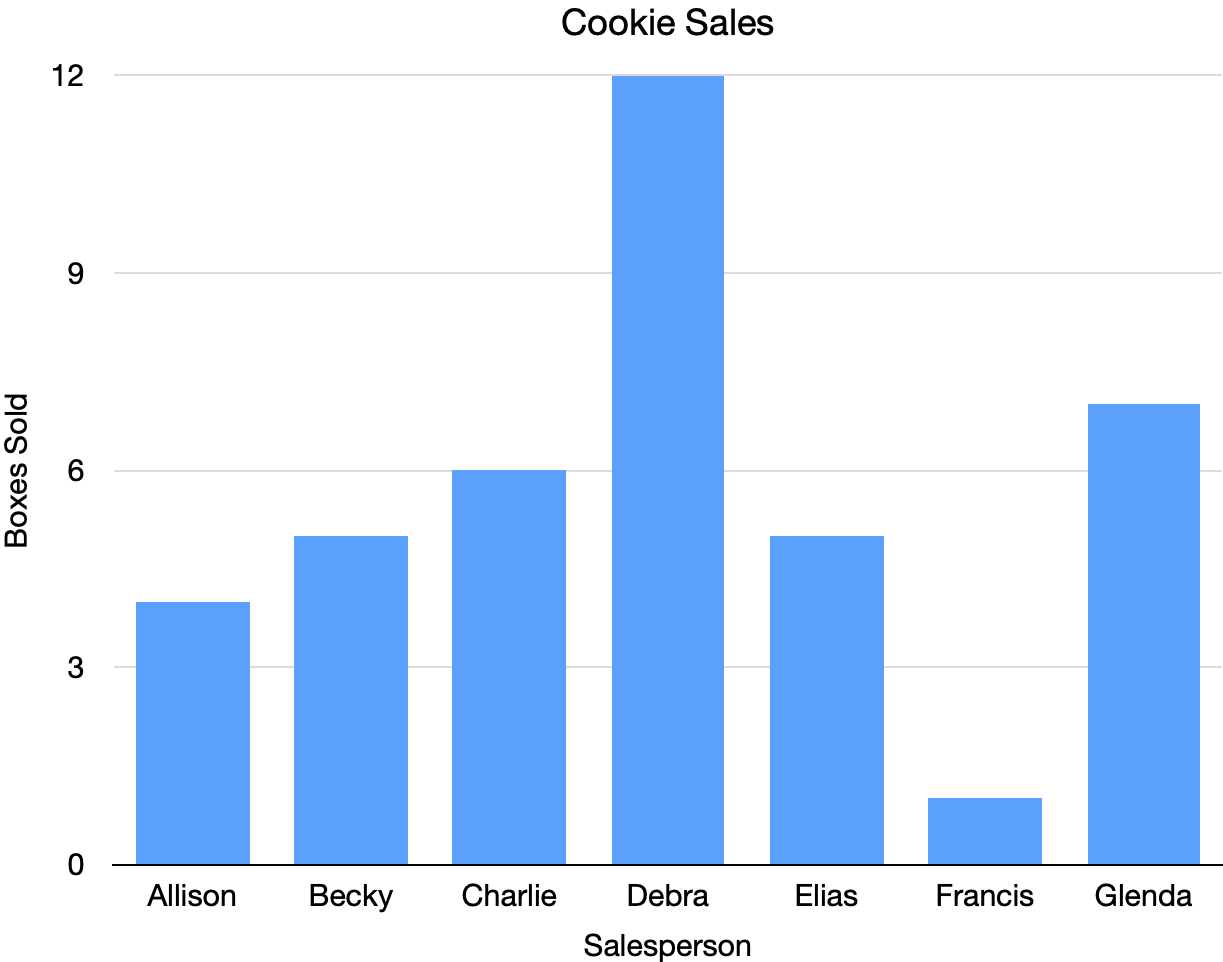
\includegraphics[width=0.7\textwidth]{CookieChart.png}

Each bar represents the cookie sales of one person. For example,
Charlie has sold 6 boxes of cookies, so the bar goes over Charlie's
name and reaches to the number 6.

Looking at this chart, you probably think, ``Wow, Debra has sold a lot
more cookies than anyone else, and Francis has sold a lot fewer.''

The same data could be in a table like this:

\begin{tabular}{c | c}
  Salesperson & Boxes Sold \\
  \hline
  Allison & 4 \\
  Becky & 5 \\
  Charlie & 6\\
  Debra & 12\\
  Elias & 5\\
  Francis & 1\\
  Glenda & 7
\end{tabular}

The table (especially a large table) is often just a bunch of
numbers. A chart helps our brains understand what the numbers mean.

Bar charts can also go horizontally.

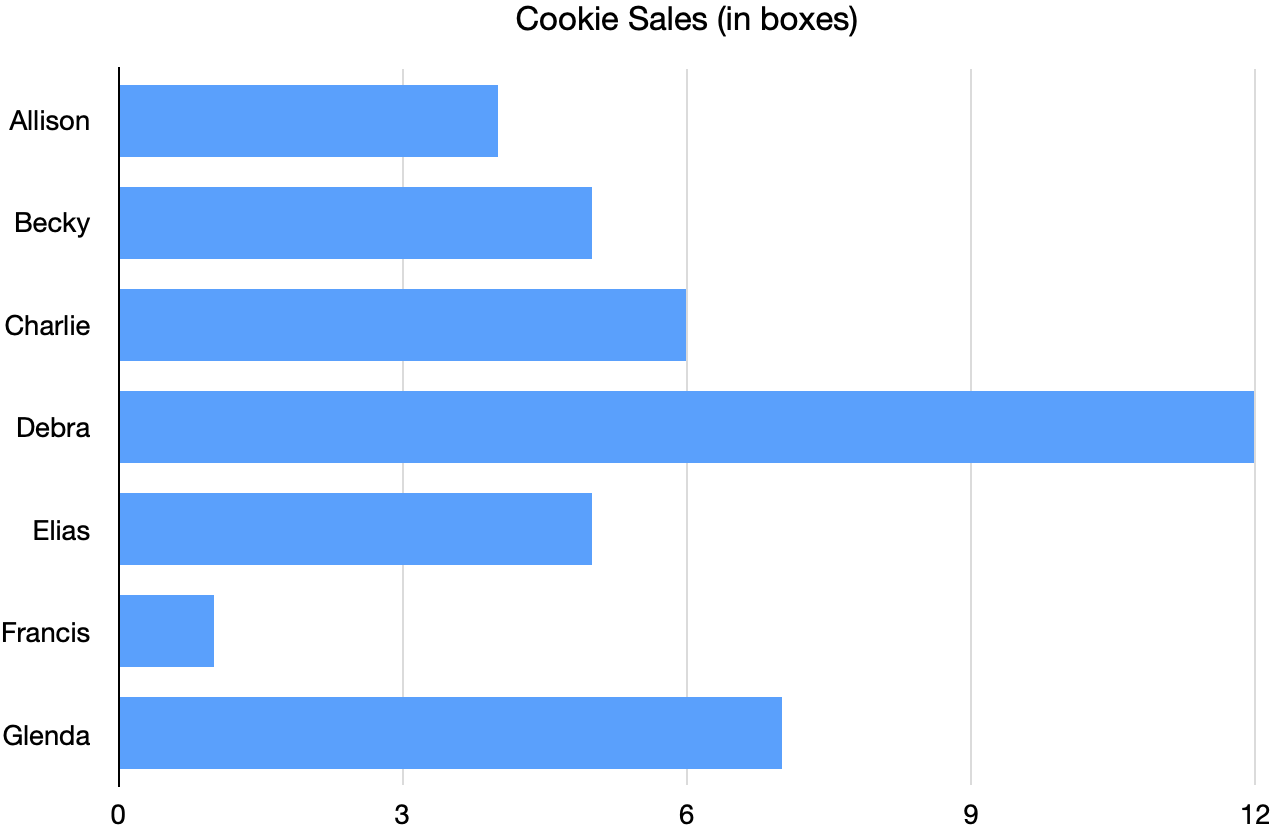
\includegraphics[width=0.7\textwidth]{HorizontalBarCookies.png}

Sometimes we use colors to explain what contributed to the number.

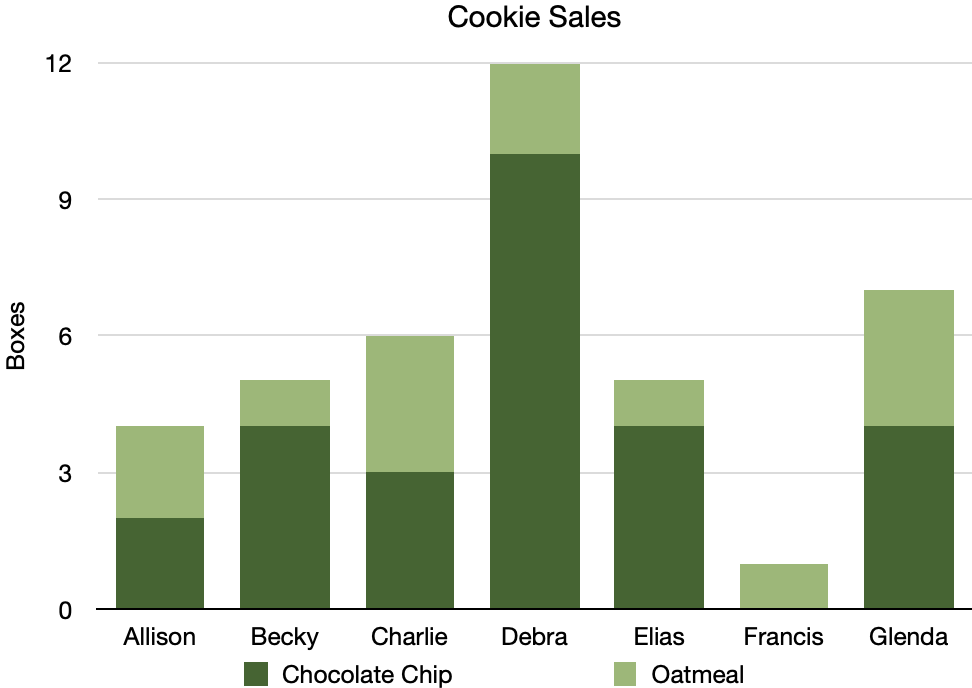
\includegraphics[width=0.7\textwidth]{TypesCookieBar.png}

This tells us that Becky sold more boxes of chocolate chip cookies
than boxes of oatmeal cookies.

\subsection{Line Graph}

Here is a line graph.\index{line graph}

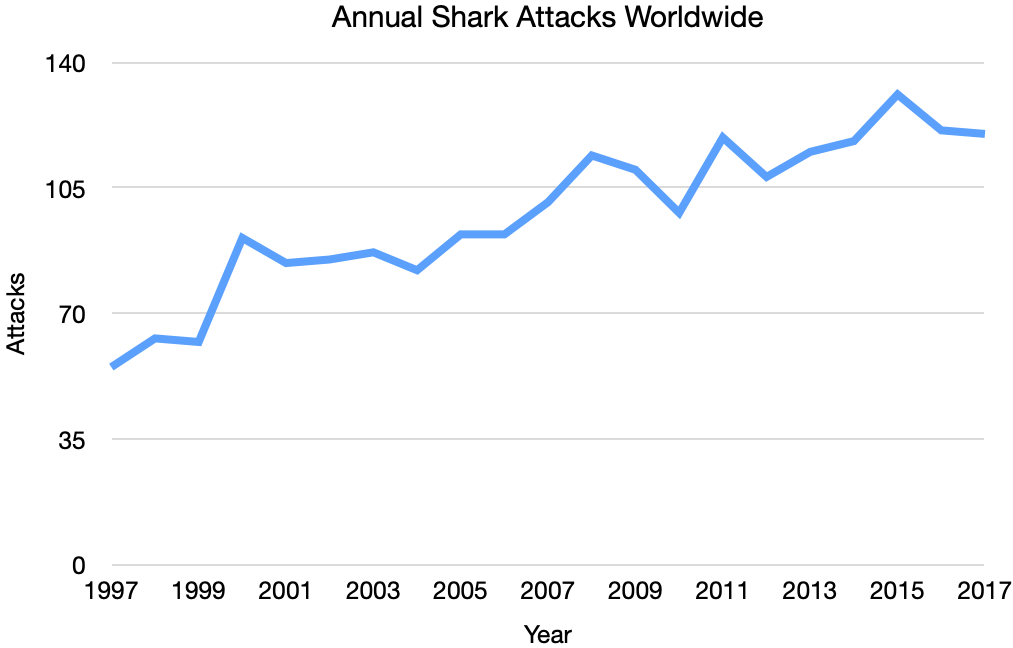
\includegraphics[width=0.7\textwidth]{SharksLine1.png}

These are often used to show trends over time. Here, for example, you
can see that the number of shark attacks has been increasing over
time.

You can have more than one line on a graph.

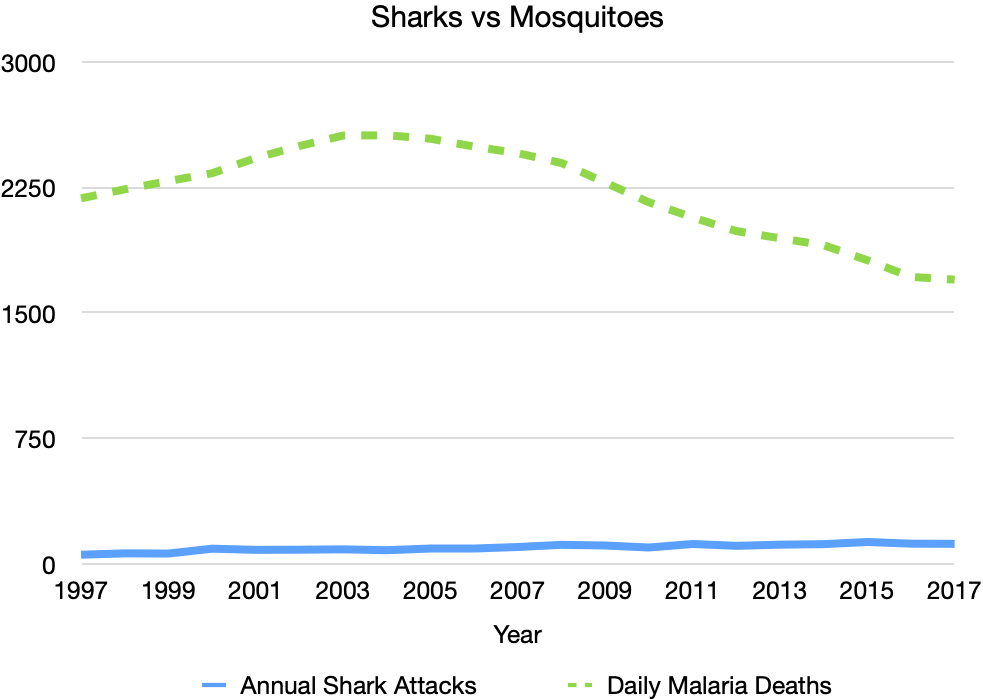
\includegraphics[width=0.7\textwidth]{SharksVsMosquitoes.png}

\subsection{Pie Chart}

You use a pie chart when you are looking at the comparative size of numbers.\index{pie chart}

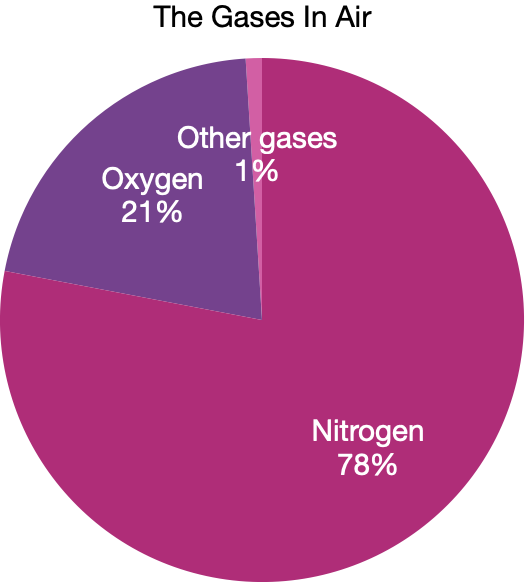
\includegraphics[width=0.4\textwidth]{AirPie.png}

\subsection{Scatter Plot}

Sometimes you have a bunch of data points with two values and you are
looking for a relationship between them.  For example, maybe you write
down the average temperature and the total sales for your lemonade
stand on the 15th of every month:\index{scatter plot}

\begin{tabular}{c | c | c}
  Date &	Avg. Temp. &	Total Sales \\
  \hline
15 January 2022 & 2.6º C & \$183.85 \\
15 February 2022 & -4.2º C & \$173.56\\
15 March 2022 & 13.3º C & \$195.22\\
15 April 2022 & 26.2º C & \$207.61\\
15 May 2022 & 27.5º C & \$210.88\\
15 June 2022 & 31.3º C & \$214.18\\
15 July 2022 & 33.5º C & \$215.23\\
15 Aug 2022 & 41.7º C & \$224.07\\
15 September 2022 & 20.7º C & \$198.94\\
15 October 2022 & 17.2º C & \$196.10\\
15 November 2022 & 1.7º C & \$185.10\\
15 December 2022 & 0.2º C & \$188.70 \\
\end{tabular}

And you think ``I wonder if I sell more lemonade on hotter days?''

You might create a scatter plot.  For each day, you put a mark that
represents that temperature and the sales that day:

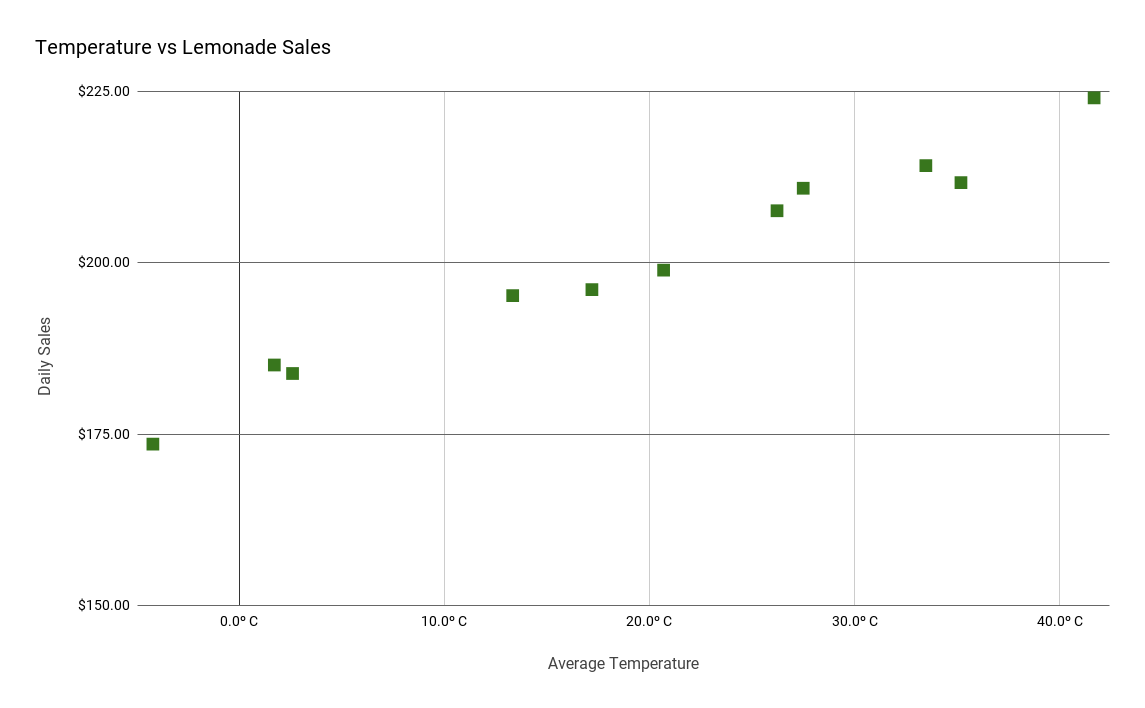
\includegraphics[width=\textwidth]{LemonadeScatter.png}

From this scatter plot, you can easily see that you do sell more
lemonade as the temperature goes up.


\section{Make Bar Graph}

Go back to your compound interest spreadsheet and make a bar graph
that shows both balances over time:

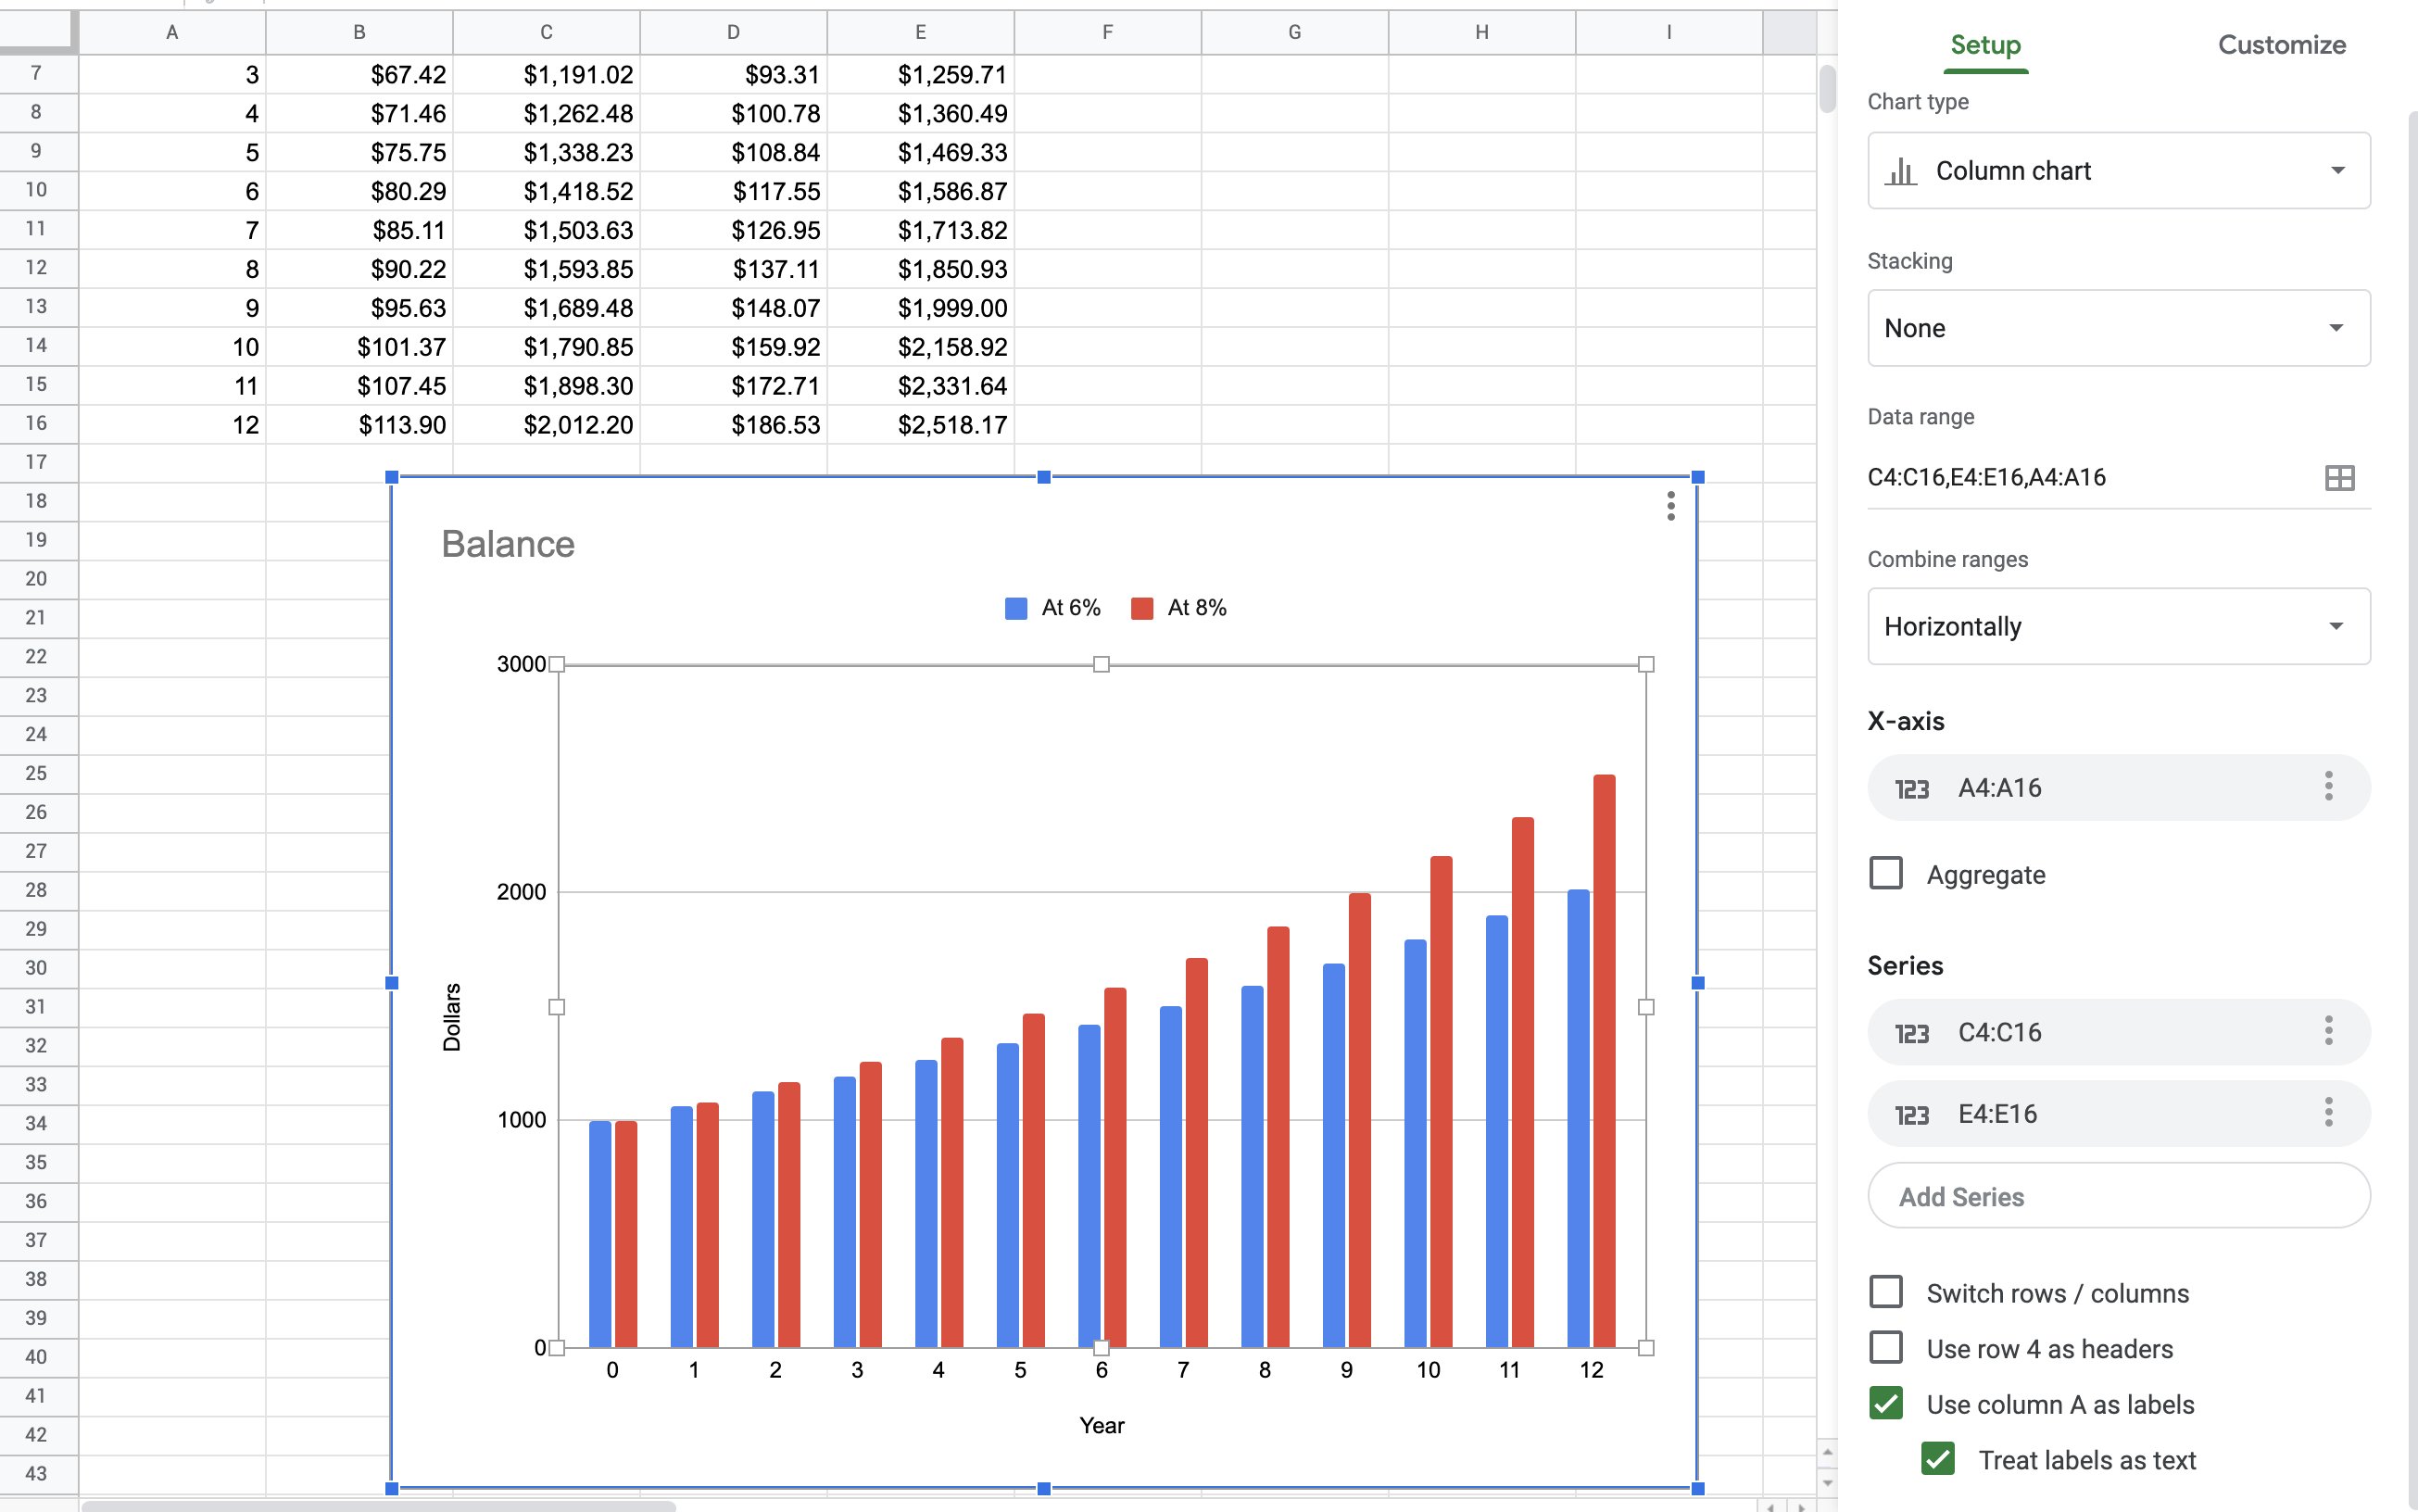
\includegraphics[width=0.9\textwidth]{InterestGraph.png}

The year column should be used as the x-axis. There are two series of
data that come from C4:C16 and E4:E16.  Tidy up the titles and legend
as much as you like.\index{spreadsheet!graphing multiple series}

Looking at the graph, you can see the balances start the same, but
balance of the account with the larger interest rate quickly pulls
away from the account with the smaller interest rate.


\chapter{Exponents}

Let's quickly review exponents. Ancient scientists started coming up
with a lot of formulas that involved multiplying the same number
several times.  For example, if they knew that if a sphere was $r$
centimeters in radius, its volume in milliliters was

$$V = \frac{4}{3} \times \pi \times r \times r \times r$$

They did two things to make the notation less messy.  First, they
decided that if two numbers were written next to each other, the
reader would assume that meant ``multiply them''.  Second, they came
up with the exponent, a little number that was lifted up off the
baseline of the text, that meant ``multiply it by itself''.  For
example $5^3$ was the same as $5 \times 5 \times 5$.\index{exponents}

Now the formula for the volume of a sphere is written

$$V = \frac{4}{3} \pi r^3$$

Tidy, right? In an exponent expression like this, we say that $r$ is
\textit{the base} and $3$ is \textit{the exponent}.

\section{Identities for Exponents}

What about exponents of exponents?  What is $\left(5^3\right)^2$?

$$\left(5^3\right)^2 = (5 \times 5 \times 5)^2 = (5 \times 5 \times 5)(5 \times 5 \times 5) = 5^6$$

In general, for any $a$, $b$, and $c$:

$$\left(a^b\right)^c = a^{(bc)}$$

If you have $\left( 5^3 \right) \left(5^4 \right)$ that is just $5 \times 5 \times 5 \times 5 \times 5 \times 5 \times 5$ or $5^7$

The general rule is, for any $a$, $b$, and $c$

$$\left(a^b\right)\left(a^c\right) = a^{(b + c)}$$

Mathematicians \textit{love} this rule, so we keep extending the idea
of exponents to keep this rule true. For example, at some point
someone asked ``What about $5^0$?'' According to the rule, $5^{2}$
must equal $5^{(2 + 0)}$ which must equal
$\left(5^2\right)\left(5^0\right)$.  Thus, $5^2$ must be 1. So
mathematicians declared ``Anything to the power of 0 is 1''.\index{exponents!zero}

Actually, we don't typically assume that $0^0 = 1$. It is just too
weird. So we say, that for any $a$ not equal to zero,

$$a^0 = 1$$

What about $5^{(-2)}$?  By our beloved rule, we know that
$\left(5^{-2}\right)\left(5^5\right)$ must be equal to $5^3$, right?
So $5^{-2}$ must be equal to $\frac{1}{5^2}$.\index{exponents!negative}

We say, for any $a$ not equal to zero and any $b$,

$$a^{-b} = \frac{1}{a^{b}}$$

This make dividing one exponentional expression by another (with the same base) easy:

$$\frac{a^b}{a^c} = a^{(b-c)}$$

We often say ``cancel out'' for this.  Here I can ``cancel out'' $x^2$:

$$\frac{x^5}{x^2} = x^3$$

What about $5^{\frac{1}{3}}$? By the beloved rule, we know that $5^{\frac{1}{3}}5^{\frac{1}{3}}5^{\frac{1}{3}}$ must equal $5^1$. Thus $5^{\frac{1}{3}} = \sqrt[3]{5}$.\index{exponents!fractions}

We say, for any $a$ and $b$ not equal to zero and any $c$ greater than zero,

$$a^{\frac{b}{c}} = a^b \sqrt[c]{a}$$

Before you go on to the exercises, note that the beloved rule demands a common base.
\begin{itemize}
\item We can combine these: $\left(5^2\right)\left(5^4\right) = 5^6$
\item We cannot combine: $\left(5^2\right)\left(3^5\right)$
\end{itemize}

With that said, we note that, for any $a$,$b$, and $c$:

$$\left(ab\right)^c = \left(a^c\right) \left(b^c\right)$$

So, for example, if I were asked to simplify
$\left(3^4\right)\left(6^2\right)$, I would note that $6 = 2 \times
3$, so

$$\left(3^4\right)\left(6^2\right) = \left(3^4\right)\left(3^2\right)\left(2^2\right)  = \left(3^6\right)\left(2^2\right)$$


If these ideas are new to you (or maybe they have been forgotten),
watch the Khan Academy's \textbf{Intro to rational exponents} video at
\url{https://youtu.be/lZfXc4nHooo}.



\chapter{Exponential Decay}

In a previous chapter, we saw that an investment of $P$ getting
compound interest with an annual interest rate of $r$, grows
exponentially. At the end of year $t$, your balance would be

$$P\left(1 + r\right)^t$$

Because $r$ is positive, this number grows as time passes.  You get a
nice exponential growth curve that looks something like this:

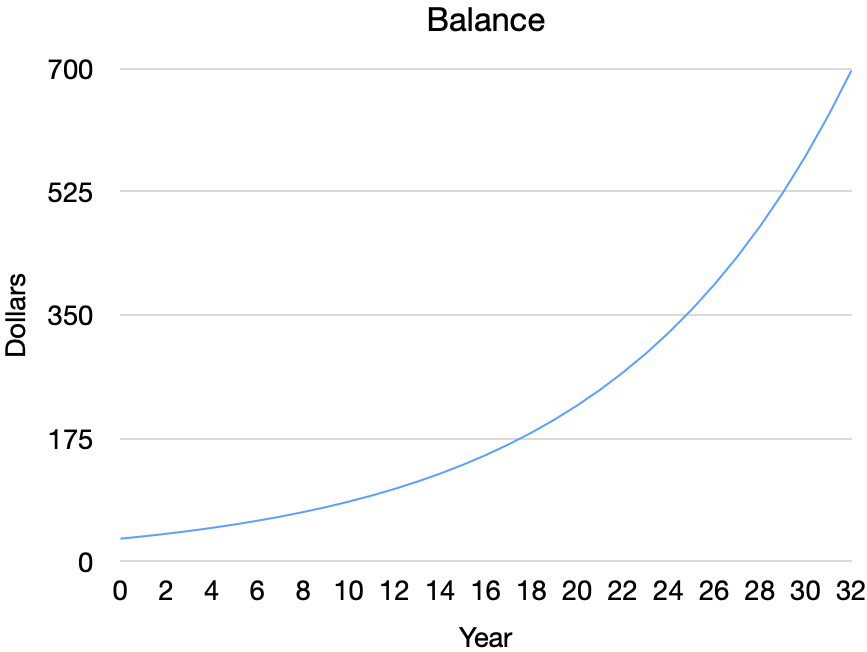
\includegraphics[width=0.7\textwidth]{exponential_growth.png}

This is \$30 invested with 10\% annual interest rate. So the formula
for the balance after $t$ years would be

$$(30)(1.1)^t$$

What if $r$ were negative? This would be \textit{exponential decay}.

\section{Radioactive Decay}

Until around 1970, there were companies making watches whose faces and
hands were coated with radioactive paint. The paint usually contained
radium. When a radium atom decays, it gives off some energy, loses two
protons and two neutrons, and becomes becomes a different element
(radon). Some of the energy given off is visible light. Thus, these
watches glow in the dark.\index{radioactive decay}

How many of the radium atoms in the paint decay each century? About 4.24\%.

Notice the quantity of atoms lost is proportional to the number of
atoms you have. This is exponential decay. If we assume that we start
with a million radium atoms, the number of atoms decreases over time like this:

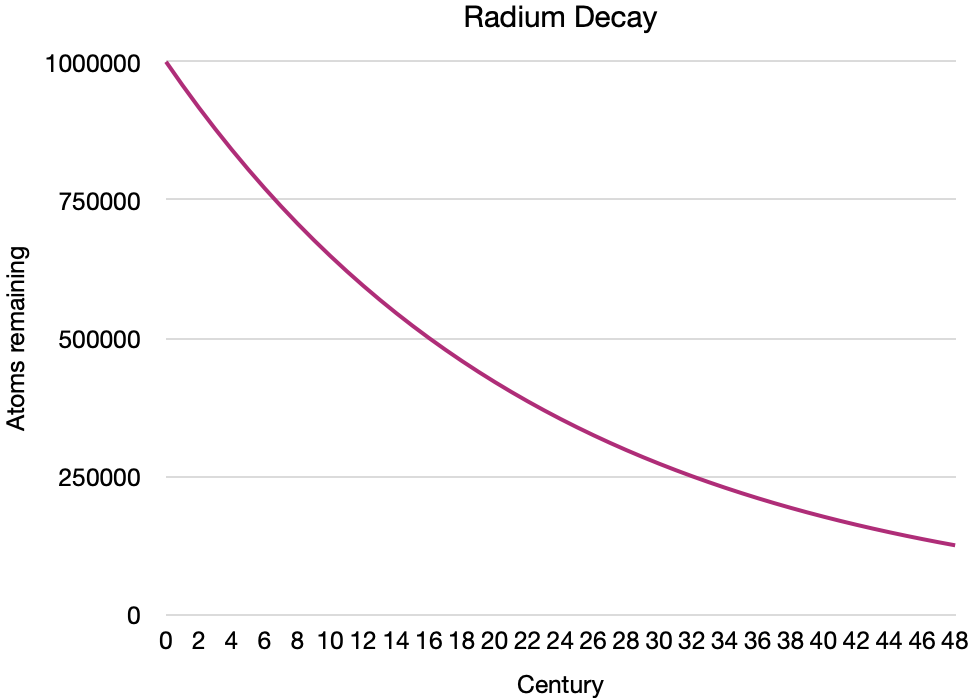
\includegraphics[width=0.7\textwidth]{radium_decay.png}
 
\begin{itemize}
\item We start off with 1,000,000 atoms.
\item At 16 centuries, we have only 500,000 (half as many) left.
\item 16 centuries after that, we have only 250,000 (half again) left.
\item 16 centures after that, we have only 125,000 (half again) left.
\end{itemize}

A nuclear chemist would say that radium has a \textit{half-life} of
1,600 years. Note that this means that if you bought a watch with
glowing hands in 1960, it will be glowing half as brightly in the year
3560.\index{half-life}

How do we calculate the amount of radium left at the end of century
$t$? If you start with $P$ atoms, at the end of the $t$-th century you
will have

$$P\left(1 - 0.0424\right)^t$$

This is exponential decay.\index{exponential decay}

\section{Model Exponential Decay}

Let's say you get hired to be run a company with 480,000
employees. Each year $1/8$ of your employees leave the company for
some reason (retirement, quitting, etc.). For some reason, you never
hire any new employees.

Make a spreadsheet that indicates how many of the original 480,000
employees will still be around at the end of each year for the next 12.  Then make a
bar graph from that data.

\chapter{Logarithms}

After the world had created exponents, it needed the opposite. We
could talk about the quantity $? = 2^3$, that is, ``What is the
product of 2 multiplied by itself three times?''  We needed some way
to talk about $2^? = 8$, that is ``2 to the what is 8?'' So we
developed the logarithm.\index{logarithm} \index{log}

Here is an example:

$$\log_{2}8 = 3$$

In English, you would say ``The logarithm base 2 of 8 is 3.''

The base (2, in this case) can be any positive number. The argument
(8, in this case) can also be any positive number.

Try this one: What is the logarthim base 2 of 1/16?

You know that $2^{-4} = \frac{1}{16}$, so $\log_{2} \frac{1}{16} = -4$.

\section{Logarithms in Python}

Most calculators have pretty limited logarithm capabilities, but
python has a nice \pyfunction{log} function that lets you specify both
the argument and the base.  Start python, import the math module, and try taking a few logarithms:\index{log!in python}

\begin{Verbatim}
>>> import math
>>> math.log(8,2)
3.0
>>> math.log(1/16, 2)
-4.0
\end{Verbatim}

Let's say that a friend offers you 5\% interest per year on your
investment for as long as you want. And you wonder, ``How many years
before my investment is 100 times as large?'' You can solve this problem with logarithms:

\begin{Verbatim}
>>> math.log(100, 1.05)
94.3872656381287
\end{Verbatim}

If you leave your investment with your friend for 94.4 years, the
investment will be worth 100 times what you put in.

\section{Logarithm Identities}

The logarithm is defined this way:\index{logarithm!identities}

$$\log_b a = c \iff b^c = a$$

Notice that the logarithm of 1 is always zero, and $\log_b b = 1$.

The logarithm of a product:

$$\log_b a c = \log_b a + \log_b c$$

This follows from the fact that $b^{a + c} = b^a b^c$. What about a quotient?

$$\log_b \frac{a}{c} = \log_b a - \log_b c$$

Exponents?

$$\log_b \left(a^c\right) = c \log_b a$$

Notice that because logs and exponents are the opposite of each other, they can cancel each other out:

$$b^{\log_b a} = a$$

and

$$\log_b \left(b^a\right) = a$$

\section{Changing Bases}

I mentioned that most calculators have pretty limited logarithm
capabilities. Most calculators don't allow you to specify what base
you want to work with. All scientific calculators have a button for
``log base 10''.  So you need to know how to use that button to get
logarithms for other bases.  Here is the change-of-base identity:\index{logarithm!change of base}

$$\log_b a = \frac {\log_c a}{\log_c b}$$

So, for example, if you wanted to find $\log_2 8$, you would ask the
calculator for $\log_{10} 8$ and then divide that by $\log_{10} 2$.
You should get 3.

\section{Natural Logarithm}

When you learn about circles, you are told that the circumference of a
circle is about 3.141592653589793 times its diameter.  Because we use
this unweildy number a lot, we give it a name: We say ``The
circumference of a circle is $\pi$ times its diameter.''

There is a second unweildy number that we will eventually use a lot in
solving problems.  It is about 2.718281828459045 (but the digits
actually go on forever, just like $\pi$). We call this number $e$. (I'm
not going to tell you why $e$ is special now, but soon...)\index{e}\index{logarithm!natural}

Most calculators have a button labeled ``ln''.  That is the
\textit{natural logarithm} button. It takes the log in base $e$.\index{ln}

Similarly, in python, if you don't specify a base, the logarithm is done in base $e$:

\begin{Verbatim}
>>> math.log(10)
2.302585092994046
>>> math.log(math.e)
1.0
\end{Verbatim}

\section{Logarithms in Spreadsheets}

Spreadsheets have three log functions:
\begin{itemize}
\item \pyfunction{LOG} takes both the argument and the base. \pyfunction{LOG(8,2)} returns 3.
\item \pyfunction{LOG10} takes just the argument and uses 10 as the base.
\item \pyfunction{LN} takes just the argument and uses $e$ as the base.
\end{itemize}

Here is a plot from a spreadsheet of a graph of $y = LOG(x, 2)$.

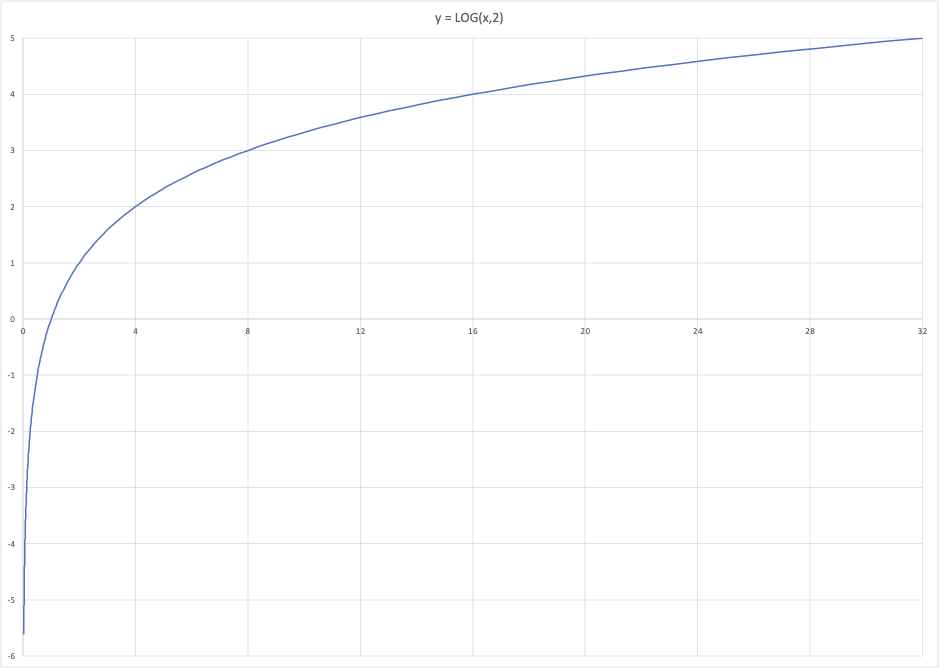
\includegraphics[width=0.8\textwidth]{log_graph.png}

Spreadsheets also have the function \pyfunction{EXP(x)} which returns
$e^x$.  For example, \pyfunction{EXP(2)} returns 7.38905609893065.


\graphicspath{{../../Modules/Oscillations/}}
\chapter{Trignometric Functions}

As mentioned earlier, in a right triangle where one angle is $\theta$,
the sine of $\theta$ is the length of the side opposite $\theta$
divided by the length of the hypotenuse.

The sine function is defined for any real number. We treat that real number
$\theta$ as an angle, we draw a ray from the origin out to the unit
circle.  The $y$ value of that point is the sine. So, for example,
the $\sin(\frac{4\pi}{3})$ is $-\sqrt{3}/2$

\begin{tikzpicture}[declare function={angle=240;},bullet/.style={inner
    sep=1pt,fill,draw,circle,solid}, scale=3]
    % Axis
    \draw[thick,-stealth,black] (-1.2,0)--(1.2,0) node[right] {$x$}; % x axis
    \draw[thick,-stealth,black] (0,-1.2)--(0,1.2) node[left] {$y$}; % y axis
    % Rest
    \draw (0,0) circle (1);
    \draw[thick] (0,0) -- (angle:1.0) node [midway, right] {1};
    \draw[sdkblue] (-0.1, 0.32) node[above] {$\theta = \frac{4\pi}{3}\text{ radians} = 240^\circ$};
    \draw[-stealth,sdkblue] (0.3,0) arc (0:angle:0.3);
    \draw[dashed, black] (-0.7, -0.866) -- (0.05, -0.866) node[right] {$\sin(\theta) = -\sqrt{3}/2$}; % horizontal
    \filldraw[black] (angle:1.0) circle(1pt);
\end{tikzpicture}

(Note that in this section, we will be using radians instead of
degrees unless otherwise noted. While degrees is more familiar to most
people, engineers and mathematicians nearly always use radians when
solving problems. Your calculator should have a radians mode and a
degrees mode. You want to be in radians mode.)

Similarly, we define cosine using the unit circle: to find the cosine
of $\theta$, we draw a ray from the origin at the angle $\theta$. The
$x$ component of the point where the ray intersects the unit circle is
the cosine of $\theta$.

\begin{tikzpicture}[declare function={angle=240;},bullet/.style={inner
    sep=1pt,fill,draw,circle,solid}, scale=3]
    % Axis
    \draw[thick,-stealth,black] (-1.2,0)--(1.2,0) node[right] {$x$}; % x axis
    \draw[thick,-stealth,black] (0,-1.2)--(0,1.2) node[left] {$y$}; % y axis
    % Rest
    \draw (0,0) circle (1);
    \draw[thick] (0,0) -- (angle:1.0) node [midway, right] {1};
    \draw[sdkblue] (0.1, 0.32) node[above] {$\theta = \frac{4\pi}{3}\text{ radians} = 240^\circ$};
    \draw[-stealth,sdkblue] (0.3,0) arc (0:angle:0.3);
    \draw[dashed, black]  (-0.5, -0.95) -- (-0.5, 0.05) node[left, above] {$\cos(\theta) = -0.5$}; % horizontal
    \filldraw[black] (angle:1.0) circle(1pt);
\end{tikzpicture}

From this description, it is easy to see why $\sin(\theta)^2 +
\cos(\theta)^2 = 1$.  They are the legs of a right triangle with a
hypotenuse of length 1.

It should also be easy to see why $\sin(\theta) = \sin(\theta +
2\pi)$: Each time you go around the circle, you come back to where
you started.

Can you see why $\cos(\theta) = \sin(\theta + \pi/2)$? Turn the picture sideways.

\section{Graphs of sine and cosine}

Here is a graph of $y = \sin(x)$:

\begin{tikzpicture}[
tl/.style = {% tick labels
    fill=white, inner sep=1pt, font=\scriptsize,
            },                        ]
% grid
\draw[sdkblue, very thin, xstep=0.5235, ystep=0.5] (-6.6,-1.2) grid (6.6,1.2);

% y tick label
\foreach \y in {-1, -1/2, 1/2, 1}{\node[tl,left=1mm] at (0,\y) {$\y$};}
% x tick label
\foreach \x [count=\xx from -4] in 
       {-2\pi,
        -\frac{3\pi}{2},
        -\pi,           
        -\frac{\pi}{2}, 
        { },
         \frac{\pi}{2},
         \pi, 
         \frac{3\pi}{2}, 
         2\pi
        }{\node[tl,below=1mm] at (3*0.5235*\xx,0) {$\x$};}
% axes
    \draw[->,thick] (-6.5,0) -- (6.5,0) node[right] {$x$};
    \draw[->,thick] (0,-1.25) -- (0, 1.25) node[above] {$y$};
% curve
\draw[<->,thick,draw=black,
      domain=-6.5:6.5,samples=300,variable=\x] 
      plot (\x,{sin(deg{\x})});
\end{tikzpicture}

It looks like waves, right? It goes forever to the left and
right. Remembering that $\cos(\theta) = \sin(\theta + \pi/2)$, we can
guess what the graph of $y = \cos(x)$ looks like:
    
\begin{tikzpicture}[
tl/.style = {% tick labels
    fill=white, inner sep=1pt, font=\scriptsize,
            },                        ]
% grid
\draw[sdkblue, very thin, xstep=0.5235, ystep=0.5] (-6.6,-1.2) grid (6.6,1.2);

% y tick label
\foreach \y in {-1, -1/2, 1/2, 1}{\node[tl,left=1mm] at (0,\y) {$\y$};}
% x tick label
\foreach \x [count=\xx from -4] in 
       {-2\pi,
        -\frac{3\pi}{2},
        -\pi,           
        -\frac{\pi}{2}, 
        { },
         \frac{\pi}{2},
         \pi, 
         \frac{3\pi}{2}, 
         2\pi
        }{\node[tl,below=1mm] at (3*0.5235*\xx,0) {$\x$};}
% axes
    \draw[->,thick] (-6.5,0) -- (6.5,0) node[right] {$x$};
    \draw[->,thick] (0,-1.25) -- (0, 1.25) node[above] {$y$};
% curve
\draw[<->,thick,draw=black,
      domain=-6.5:6.5,samples=300,variable=\x] plot (\x,{cos(deg{\x})});
\end{tikzpicture}

\section{Plot cosine in Python}

Create a file called \filename{cos.py}:

\begin{Verbatim}
import numpy as np
import matplotlib.pyplot as plt

until = 8.0

# Make a plot of cosine
thetas = np.linspace(0, until, 32)
cosines = []
for theta in thetas:
    cosines.append(np.cos(theta))

# Plot the data
fig, ax = plt.subplots()
ax.plot(thetas, cosines, 'r.', label="Cosine")
ax.set_title("Cosine")
plt.show()
\end{Verbatim}

This will plot 32 points on the cosine wave between 0 and 8.  When you
run it, you should see something like this:

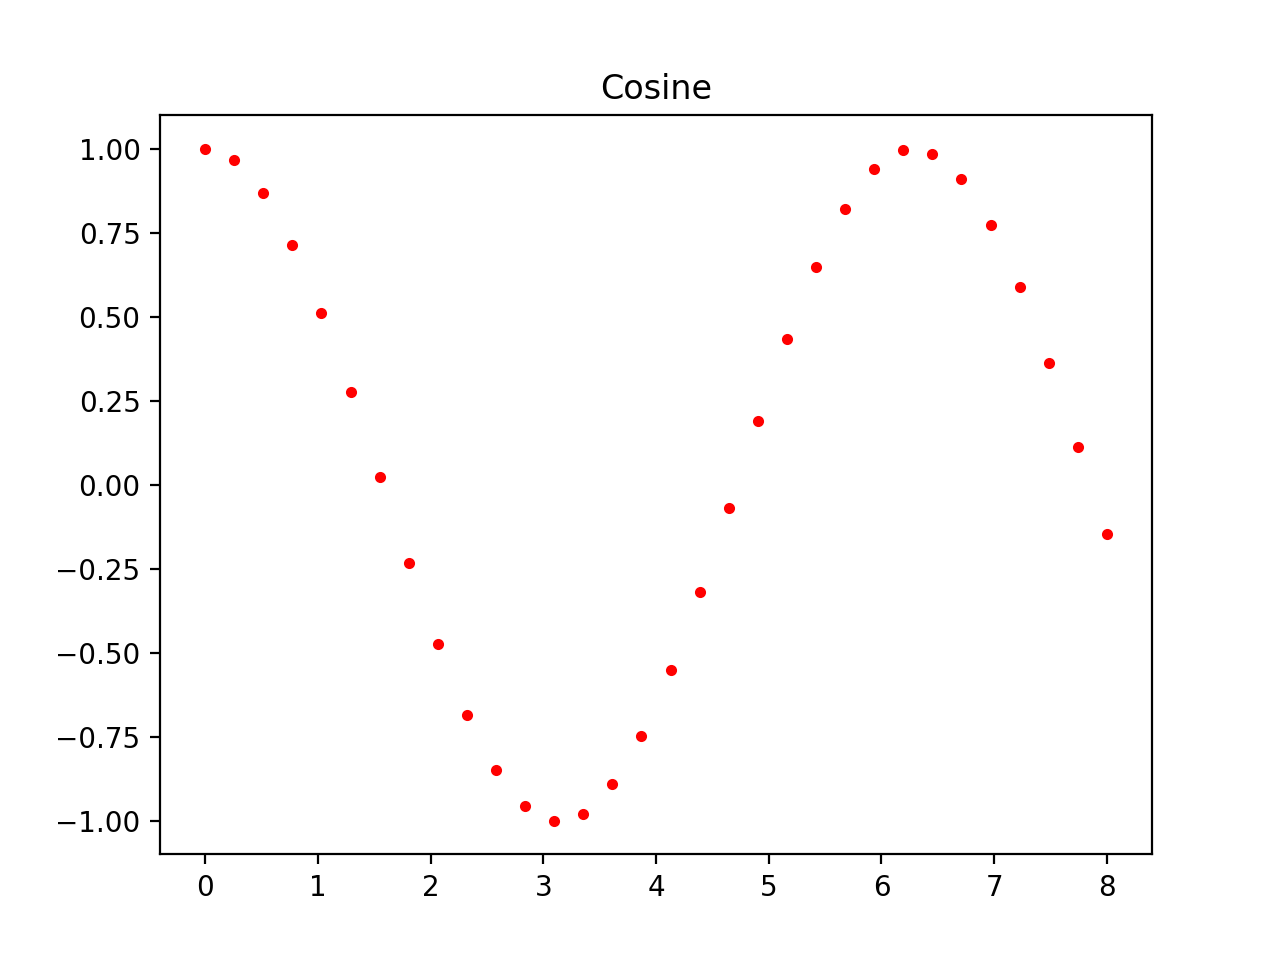
\includegraphics[width=0.8\textwidth]{cospy.png}

\section{Derivatives of sine and cos}

Here is a wonderful property of sine and cosine functions: At any point $\theta$, the slope of the sine graph at $\theta$ equals $cos(\theta)$.

For example, we know that $\sin(4\pi/3) = -(1/2)\sqrt{3}$ and
$\cos(4\pi/3) = -1/2$. If we drew a line tangent to the sine curve at
this point, it would have a slope of -1/2:

\begin{tikzpicture}[
tl/.style = {% tick labels
    fill=white, inner sep=1pt, font=\scriptsize,
            },                        ]
% grid
\draw[sdkblue, very thin, xstep=0.5235, ystep=0.5] (-1.25,-1.7) grid (6.6,1.2);

% y tick label
\foreach \y in {-3/2, -1, -1/2, 1/2, 1}{\node[tl,left=1mm] at (0,\y) {$\y$};}
% x tick label
\foreach \x [count=\xx from -1] in 
       {-\frac{\pi}{2}, 
        { },
         \frac{\pi}{2},
         \pi, 
         \frac{3\pi}{2}, 
         2\pi
        }{\node[tl,below=1mm] at (3*0.5235*\xx,0) {$\x$};}
% axes
    \draw[->,thick] (-1.25,0) -- (6.5,0) node[right] {$x$};
    \draw[->,thick] (0,-1.5) -- (0, 1.25) node[above] {$y$};
% curve
\draw[<->,thick,draw=black,
      domain=-1.75:6.5,samples=300,variable=\x] 
      plot (\x,{sin(deg{\x})});
\filldraw[black] (4.188790204786391,-0.866025403784439) circle(2pt);
\draw[->, thick, draw=red] (4.188790204786391,-0.866025403784439) -- (5.188790204786391,-1.366025403784439) node [right] {slope = -1/2} ;
\end{tikzpicture}

We say ``The derivative of the sine function is the cosine function.''

Can you guess the derivative of the cosine function? For any $\theta$, the slope of the graph of the $\cos(\theta)$ is $-\sin(\theta)$.



\section{A weight on a spring}

Let's say you fill a rollerskate with heavy rocks and attach it to the
wall with a stiff spring.  If you push the skate toward the wall a
release it, it will roll back and forth. Engineers would say ``The skate will oscillate.''

Intuitively, you can probably guess:
\begin{itemize}
\item If the spring is stronger, the skate will oscillate more times per minute.
\item If the rocks are lighter, the skate will oscillate more times per minute.
\end{itemize}

The force that the spring exerts on the skate is proportional to how
far its length is from its relaxed length.. When you buy a spring, the
manufacturer advertises its ``spring rate'', which is in pounds per
inch or newtons per meter.  If a spring has a rate of 5 newtons per
meter, that means that if stretch or compress it 10 cm, it will push
back with a force of 0.5 newtons. If you stretch or compress it 20 cm,
it will push back with a force of 1 newton.

Let's write a simulation of the skate-on-a-spring.  Duplicate \filename{cos.py}, and name the new copy \filename{spring.py}.  Add code to implement the simulation:

\begin{Verbatim}[commandchars=\\\{\}]
import numpy as np
import matplotlib.pyplot as plt

until = 8.0

\textbf{# Constants}
\textbf{mass = 100 # kg}
\textbf{spring_constant = -1 # newtons per meter displacement}
\textbf{time_step = 0.01 # s}

\textbf{# Initial state}
\textbf{displacement = 1.0 # height above equilibrium in meters}
\textbf{velocity = 0.0}
\textbf{time = 0.0 # seconds}

\textbf{# Lists to gather data}
\textbf{displacements = []}
\textbf{times = []}

\textbf{# Run it for a little while}
\textbf{while time <= until:}
\textbf{    # Record data}
\textbf{    displacements.append(displacement)}
\textbf{    times.append(time)}

\textbf{    # Calculate the next state}
\textbf{    time += time_step}
\textbf{    displacement += time_step * velocity}
\textbf{    force = spring_constant * displacement }
\textbf{    acceleration = force / mass}
\textbf{    velocity += acceleration}

# Make a plot of cosine
thetas = np.linspace(0, until, 32)
cosines = []
for theta in thetas:
    cosines.append(np.cos(theta))

# Plot the data
fig, ax = plt.subplots()
\textbf{ax.plot(times, displacements, 'b', label="Displacement")}
ax.plot(thetas, cosines, 'r.', label="Cosine")

\textbf{ax.set_title("Weight on Spring vs. Cosine")}
\textbf{ax.set_xlabel("Time (s)")}
\textbf{ax.set_ylabel("Displacement (m)")}
\textbf{ax.legend()}
plt.show()
\end{Verbatim}
When you run it, you should get a plot of your spring and the cosine graph on the same plot.

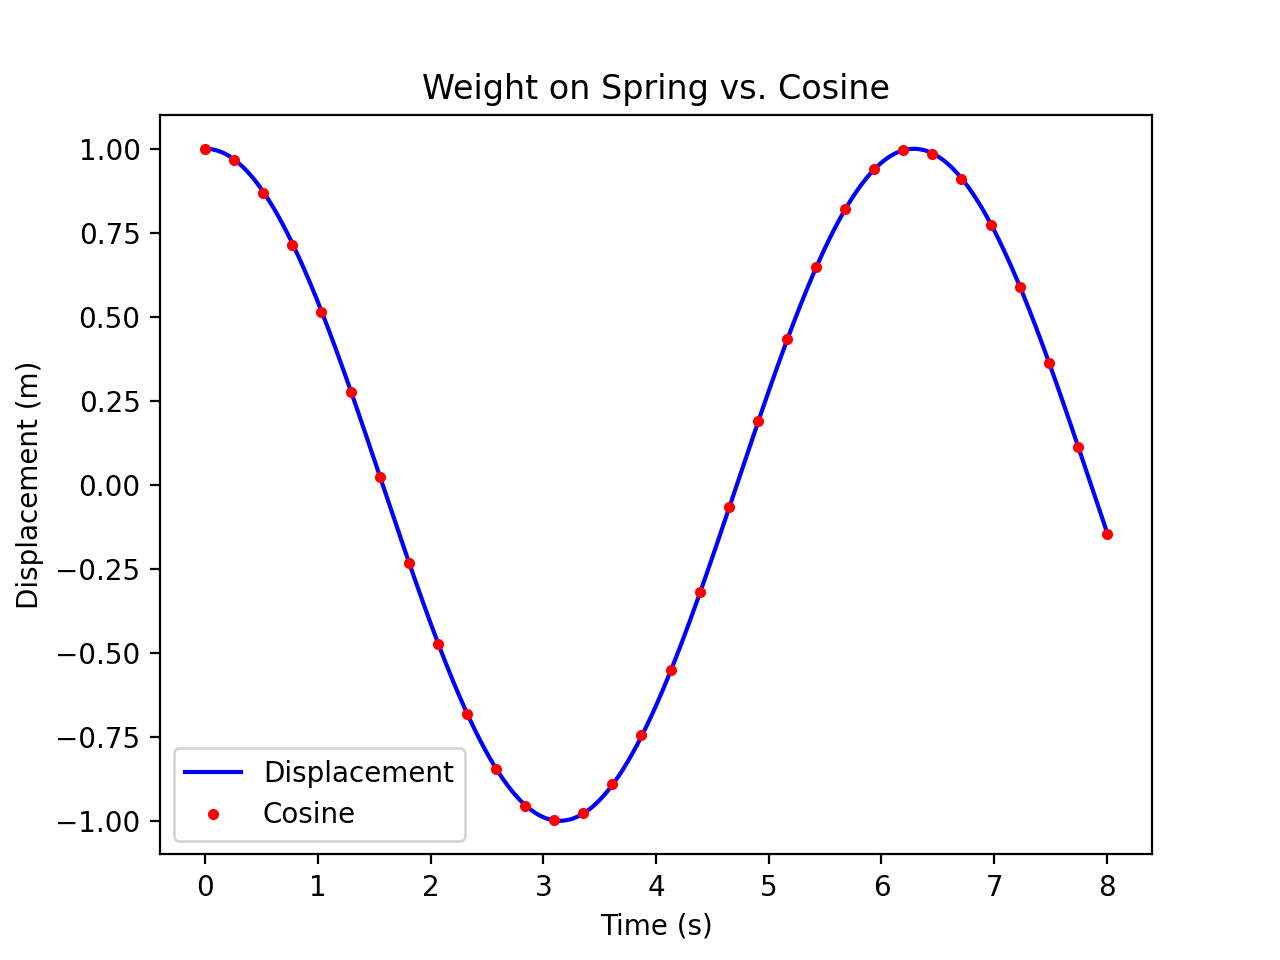
\includegraphics[width=0.8\textwidth]{springpy.png}

The position of the skate is following a cosine curve. Why?

Because for a sine or cosine waves happen whenever the acceleration of 
an object is proportional to -1 times its displacement. Or in symbols:

$$a \propto -1 * p$$

where $a$ is acceleration and $p$ is the displacement from equilibrum.

Remember that if you take the derivative of the displacement, you get
the velocity.  And if you take the derivative of that, you get
acceleration.  So, the weight on the spring must follow a function $f$ such that

$$f(t) \propto -1 * f''(t)$$

Remember that the derivative of the $\sin(\theta)$ is $\cos(\theta)$.

And the derivative of the $\cos(\theta)$ is $- \sin(\theta)$

Thus these sorts of waves have an almost-magical power: their
acceleration is proportional to -1 times their displacement.

Thus sine waves of various magnitudes and frequencies are ubiquitous
in nature and technology.

\section{Integral of sine and cosine}

If we take the area between the graph and the $x$ axis of the cosine
function (and if the function is below the $x$ axis, it counts as
negative area), from 0 to $4\pi/3$, we find that it is equal to
$-(1/2)\sqrt{3}$

\begin{tikzpicture}[
tl/.style = {% tick labels                                                                                               
    fill=white, inner sep=1pt, font=\scriptsize,
            },                        ]

% y tick label                                                                                                           
\foreach \y in {-1, -1/2, 1/2, 1}{\node[tl,left=1mm] at (0,\y) {$\y$};}
% x tick label                                                                                                           
\foreach \x [count=\xx from -1] in
       {-\frac{\pi}{2},
        { },
         \frac{\pi}{2},
         \pi,
         \frac{3\pi}{2},
         2\pi
        }{\node[tl,below=1mm] at (3*0.5235*\xx,0) {$\x$};}
       % axes
       \draw[->,thick] (-1.25,0) -- (6.5,0) node[right] {$x$};
       \draw[->,thick] (0,-1.25) -- (0, 1.25) node[above] {$y$};
       % curve
       \draw[<->,thick,draw=black, domain=-1.75:6.5,samples=300,variable=\x] plot (\x,{cos(deg{\x})});
       \fill[sdkblue, domain=0:1.57,samples=100, variable=\b]
       (0, 1)
       -- plot (\b,{cos(deg(\b))})
       -- (0, 0)
       -- cycle;
       \fill[red, domain=1.57:4.188790204786391,samples=100, variable=\b]
       (1.57, 0)
       -- plot (\b,{cos(deg(\b))})
       -- (4.188790204786391, 0)
       -- cycle;
       \draw[thick, draw=black] (4.188790204786391, 1) -- (4.188790204786391,-1) node [right]{area=$-(1/2)\sqrt{3}$};
\end{tikzpicture}

We say ``The integral of the cosine function is the sine function.'' 











\chapter{Transforming Functions}

Let's say I gave you the graph of a function $f$, like this:

\begin{tikzpicture}
    \begin{axis}[
        xmin=-2.2,xmax=2.2,
        ymin=-1,ymax=5,
        axis x line=middle,
        axis y line=middle,
        axis line style=<->,
        xlabel={$x$},
        ylabel={$y$},
      ]
      \addplot[no marks,sdkblue] expression[domain=-2:2,samples=100]{x^2} node[below, yshift=-6mm] {$f(x)$};
    \end{axis}\end{tikzpicture}

And then I tell you that the function $g(x) = f(x) + 1.5$.  Can you guess what the graph of $g$ would look like? It is the same graph, just translated up 1.5:

\begin{tikzpicture}
    \begin{axis}[
        xmin=-2.2,xmax=2.2,
        ymin=-1,ymax=5,
        axis x line=middle,
        axis y line=middle,
        axis line style=<->,
        xlabel={$x$},
        ylabel={$y$},
      ]
      \addplot[dashed,sdkblue] expression[domain=-2:2,samples=100]{x^2} node[below, yshift=-6mm] {$f(x)$};
      \addplot[no marks,sdkblue] expression[domain=-2:2,samples=100]{x^2 + 1.5} node[below, yshift=-6mm] {$g(x)$};
    \end{axis}\end{tikzpicture}

There are four kinds of transformations that we do all the time:
\begin{itemize}
\item Translation up and down in the direction of $y$ axis (the one you just saw)
\item Translation left and right in the direciton of the $x$ axis
\item Scaling up and down along the $y$ axis
\item Scaling up and down along the $x$ axis
\end{itemize}

Now I will demonstrate each of the four using the graph of $\sin(x)$.

\subsection{Translation up and down}

When you add a positive constant to a function, you translate the
whole graph up that much. A negative constant translates it down.

Here is the graph of $\sin(x) - 0.5$:

\begin{tikzpicture}[
tl/.style = {% tick labels
    fill=white, inner sep=1pt, font=\scriptsize,
            },                        ]
% grid
\draw[sdkblue, very thin, xstep=0.5235, ystep=0.5] (-6.6,-1.7) grid (6.6,1.2);

% y tick label
\foreach \y in {-1, -1/2, 1/2, 1}{\node[tl,left=1mm] at (0,\y) {$\y$};}
% x tick label
\foreach \x [count=\xx from -4] in 
       {-2\pi,
        -\frac{3\pi}{2},
        -\pi,           
        -\frac{\pi}{2}, 
        { },
         \frac{\pi}{2},
         \pi, 
         \frac{3\pi}{2}, 
         2\pi
        }{\node[tl,below=1mm] at (3*0.5235*\xx,0) {$\x$};}
% axes
    \draw[->,thick] (-6.5,0) -- (6.5,0) node[right] {$x$};
    \draw[->,thick] (0,-1.25) -- (0, 1.25) node[above] {$y$};
% curve
\draw[<->,dashed,draw=black,
      domain=-6.5:6.5,samples=300,variable=\x] 
      plot (\x,{sin(deg{\x})});
\draw[<->,thick,draw=black,
      domain=-6.5:6.5,samples=300,variable=\x] 
      plot (\x,{sin(deg{\x}) - 0.5});
\end{tikzpicture}

\subsection{Translation left and right}

When you add a positive number to $x$ before running it through $f$,
you translate the graph to the left that much. Adding a negative
number translates the graph to the right.

Here is the graph of $\sin(x - \pi/6)$:

\begin{tikzpicture}[
tl/.style = {% tick labels
    fill=white, inner sep=1pt, font=\scriptsize,
            },                        ]
% grid
\draw[sdkblue, very thin, xstep=0.5236, ystep=0.5] (-6.6,-1.2) grid (6.6,1.2);

% y tick label
\foreach \y in {-1, -1/2, 1/2, 1}{\node[tl,left=1mm] at (0,\y) {$\y$};}
% x tick label
\foreach \x [count=\xx from -4] in 
       {-2\pi,
        -\frac{3\pi}{2},
        -\pi,           
        -\frac{\pi}{2}, 
        { },
         \frac{\pi}{2},
         \pi, 
         \frac{3\pi}{2}, 
         2\pi
        }{\node[tl,below=1mm] at (3*0.5235*\xx,0) {$\x$};}
% axes
    \draw[->,thick] (-6.5,0) -- (6.5,0) node[right] {$x$};
    \draw[->,thick] (0,-1.25) -- (0, 1.25) node[above] {$y$};
% curve
\draw[<->,dashed,draw=black,
      domain=-6.5:6.5,samples=300,variable=\x] 
      plot (\x,{sin(deg{\x})});
\draw[<->,thick,draw=black,
      domain=-6.5:6.5,samples=300,variable=\x] 
      plot (\x,{sin(deg{\x} - 30)});
\end{tikzpicture}

Notice the sign:
\begin{itemize}
\item Add to $x$ before processing with the function translates the graph to the \emph{left}.
\item Subtract from $x$ before processing with the function translates the graph to the \emph{right}
\end{itemize}

\subsection{Scaling up and down in the $y$ direction}

To scale the function up and down, you multiply the result of the
function by a constant.  If the constant is larger than 1, it
stretches the function up and down.

Here is $y = 2\sin(x)$:

\begin{tikzpicture}[
tl/.style = {% tick labels
    fill=white, inner sep=1pt, font=\scriptsize,
            },                        ]
% grid
\draw[sdkblue, very thin, xstep=0.5236, ystep=0.5] (-6.6,-2.2) grid (6.6,2.2);

% y tick label
\foreach \y in {-1, -1/2, 1/2, 1}{\node[tl,left=1mm] at (0,\y) {$\y$};}
% x tick label
\foreach \x [count=\xx from -4] in 
       {-2\pi,
        -\frac{3\pi}{2},
        -\pi,           
        -\frac{\pi}{2}, 
        { },
         \frac{\pi}{2},
         \pi, 
         \frac{3\pi}{2}, 
         2\pi
        }{\node[tl,below=1mm] at (3*0.5235*\xx,0) {$\x$};}
% axes
    \draw[->,thick] (-6.5,0) -- (6.5,0) node[right] {$x$};
    \draw[->,thick] (0,-1.25) -- (0, 1.25) node[above] {$y$};
% curve
\draw[<->,dashed,draw=black,
      domain=-6.5:6.5,samples=300,variable=\x] 
      plot (\x,{sin(deg{\x})});
\draw[<->,thick,draw=black,
      domain=-6.5:6.5,samples=300,variable=\x] 
      plot (\x,{sin(deg{\x}) * 2.0});
\end{tikzpicture}

With a wave like this, we speak of its \newterm{Amplitude}, which you
can think of as its height. The baseline that this wave oscillates
around is zero. The maximum distance that it gets from that baseline
is its amplitude.  Thus, the amplitude here has been increased from 1
to 2.

If you multiply by a negative number, the function gets flipped.  Here is $y = -0.5 \sin(x)$

\begin{tikzpicture}[
tl/.style = {% tick labels
    fill=white, inner sep=1pt, font=\scriptsize,
            },                        ]
% grid
\draw[sdkblue, very thin, xstep=0.5236, ystep=0.5] (-6.6,-1.2) grid (6.6,1.2);

% y tick label
\foreach \y in {-1, -1/2, 1/2, 1}{\node[tl,left=1mm] at (0,\y) {$\y$};}
% x tick label
\foreach \x [count=\xx from -4] in 
       {-2\pi,
        -\frac{3\pi}{2},
        -\pi,           
        -\frac{\pi}{2}, 
        { },
         \frac{\pi}{2},
         \pi, 
         \frac{3\pi}{2}, 
         2\pi
        }{\node[tl,below=1mm] at (3*0.5235*\xx,0) {$\x$};}
% axes
    \draw[->,thick] (-6.5,0) -- (6.5,0) node[right] {$x$};
    \draw[->,thick] (0,-1.25) -- (0, 1.25) node[above] {$y$};
% curve
\draw[<->,dashed,draw=black,
      domain=-6.5:6.5,samples=300,variable=\x] 
      plot (\x,{sin(deg{\x})});
\draw[<->,thick,draw=black,
      domain=-6.5:6.5,samples=300,variable=\x] 
      plot (\x,{sin(deg{\x}) * -0.5});
\end{tikzpicture}

Amplitude is never negative.  Thus, the amplitude of this wave is 0.5.

\subsection{Scaling up and down in the $x$ direction}

If you multiply $x$ by a number larger than 1 before running it
through the function, the graph gets compressed toward zero.

Here is $y = 3 \sin(x)$:

\begin{tikzpicture}[
tl/.style = {% tick labels
    fill=white, inner sep=1pt, font=\scriptsize,
            },                        ]
% grid
\draw[sdkblue, very thin, xstep=0.5236, ystep=0.5] (-6.6,-1.2) grid (6.6,1.2);

% y tick label
\foreach \y in {-1, -1/2, 1/2, 1}{\node[tl,left=1mm] at (0,\y) {$\y$};}
% x tick label
\foreach \x [count=\xx from -4] in 
       {-2\pi,
        -\frac{3\pi}{2},
        -\pi,           
        -\frac{\pi}{2}, 
        { },
         \frac{\pi}{2},
         \pi, 
         \frac{3\pi}{2}, 
         2\pi
        }{\node[tl,below=1mm] at (3*0.5235*\xx,0) {$\x$};}
% axes
    \draw[->,thick] (-6.5,0) -- (6.5,0) node[right] {$x$};
    \draw[->,thick] (0,-1.25) -- (0, 1.25) node[above] {$y$};
% curve
\draw[<->,dashed,draw=black,
      domain=-6.5:6.5,samples=300,variable=\x] 
      plot (\x,{sin(deg{\x})});
\draw[<->,thick,draw=black,
      domain=-6.5:6.5,samples=300,variable=\x] 
      plot (\x,{sin(deg{\x} * 3)});
\end{tikzpicture}

The distance between two peaks of a wave is known as its
\newterm{wavelength}.  The original wave had a wavelength of $2\pi$.
The compressed wave has a wavelength of $2\pi/3$.

If you multiply $x$ by a number smaller than 1, it will stretch the function out, away from the $y$ axis.

If you multiply $x$ by a negative number, it will flip the function around the $y$ axis.

Here is $y = 2^{(-0.5x)}$. Notice that it has flipped around the $y$ axis and is stretched out along the $x$ axis.

\begin{tikzpicture}
    \begin{axis}[
        xmin=-3.1,xmax=3.1,
        ymin=-0.5,ymax=8,
        axis x line=middle,
        axis y line=middle,
        axis line style=<->,
        xlabel={$x$},
        ylabel={$y$},
      ]
      \addplot[dashed,sdkblue] expression[domain=-3.0:3.0,samples=100]{2^x} node[left, xshift=-1mm,yshift=-6mm] {$2^x$};
      \addplot[no marks,sdkblue] expression[domain=-3.0:3.0,samples=100]{2^(-0.5 * x)}
      node[above, xshift=-6mm] {$2^{-0.5x}$};
    \end{axis}\end{tikzpicture}

\subsection{Order is important!}

We can combine these transformations. This allows us, for example, to
translate a function up 2 and then scale along the $y$ axis by 3.

Here is $y = 2.0 (\sin(x) + 1)$:

\begin{tikzpicture}[
tl/.style = {% tick labels
    fill=white, inner sep=1pt, font=\scriptsize,
            },                        ]
% grid
\draw[sdkblue, very thin, xstep=0.5236, ystep=0.5] (-6.6,-1.2) grid (6.6,4.2);

% y tick label
\foreach \y in {-1, -1/2, 1/2, 1, 2, 3, 4}{\node[tl,left=1mm] at (0,\y) {$\y$};}
% x tick label
\foreach \x [count=\xx from -4] in 
       {-2\pi,
        -\frac{3\pi}{2},
        -\pi,           
        -\frac{\pi}{2}, 
        { },
         \frac{\pi}{2},
         \pi, 
         \frac{3\pi}{2}, 
         2\pi
        }{\node[tl,below=1mm] at (3*0.5235*\xx,0) {$\x$};}
% axes
    \draw[->,thick] (-6.5,0) -- (6.5,0) node[right] {$x$};
    \draw[->,thick] (0,-1.25) -- (0, 4.25) node[above] {$y$};
% curve
\draw[<->,dashed,draw=black,
      domain=-6.5:6.5,samples=300,variable=\x] 
      plot (\x,{sin(deg{\x})});
\draw[<->,thick,draw=black,
      domain=-6.5:6.5,samples=300,variable=\x] 
      plot (\x,{2.0 * (sin(deg{\x}) + 1)});
\end{tikzpicture}

A function is often a series of steps. Here are the steps in $f(x) = 2(\sin(x) + 1)$:
\begin{enumerate}
\item Take the sine of $x$
\item Add 1 to that
\item Multiply that by 2
\end{enumerate}

What if we change the order? Here are the steps in $g(x) = 2\sin(x) + 1$:
\begin{enumerate}
\item Take the sine of $x$
\item Multiply that by 2
\item Add 1 to that
\end{enumerate}

\begin{tikzpicture}[
tl/.style = {% tick labels
    fill=white, inner sep=1pt, font=\scriptsize,
            },                        ]
% grid
\draw[sdkblue, very thin, xstep=0.5236, ystep=0.5] (-6.6,-2.2) grid (6.6,4.2);

% y tick label
\foreach \y in {-2, -1, -1/2, 1/2, 1, 2, 3, 4}{\node[tl,left=1mm] at (0,\y) {$\y$};}
% x tick label
\foreach \x [count=\xx from -4] in 
       {-2\pi,
        -\frac{3\pi}{2},
        -\pi,           
        -\frac{\pi}{2}, 
        { },
         \frac{\pi}{2},
         \pi, 
         \frac{3\pi}{2}, 
         2\pi
        }{\node[tl,below=1mm] at (3*0.5235*\xx,0) {$\x$};}
% axes
    \draw[->,thick] (-6.5,0) -- (6.5,0) node[right] {$x$};
    \draw[->,thick] (0,-2.25) -- (0, 4.25) node[above] {$y$};
% curve
\draw[<->,dashed,draw=black,
      domain=-6.5:6.5,samples=300,variable=\x] 
plot (\x,{2.0 * (sin(deg{\x}) + 1)});
\draw (4, 3) node{$2(\sin(x) + 1)$};
\draw[<->,thick,draw=black,
      domain=-6.5:6.5,samples=300,variable=\x] 
      plot (\x,{2.0 * sin(deg{\x} + 1)});
\draw (2.5, -1.5) node{$2\sin(x) + 1$};
\end{tikzpicture}

The moral: You can do multiple transformations of your function, but
the order in which you do them is important.

\begin{Exercise}[title={Transforms}, label=sine_transform]

Find a function that creates a sine wave such that the top of the first crest is
at the point $(\frac{\pi}{2}, 5)$ and the bottom of the trough that follows is at $(\pi, 1)$.


\begin{tikzpicture}[
tl/.style = {% tick labels
    fill=white, inner sep=1pt, font=\scriptsize,
            },                        ]
% grid
\draw[sdkblue, very thin, xstep=0.5236, ystep=0.5] (-1,-0.6) grid (6.6,5.2);

% y tick label
\foreach \y in {1/2, 1, 2, 3, 4, 5}{\node[tl,left=1mm] at (0,\y) {$\y$};}
% axes
    \draw[->,thick] (-0.9,0) -- (6.5,0) node[right] {$x$};
    \draw[->,thick] (0,-0.25) -- (0, 5.25) node[above] {$y$};
    % curve
    \filldraw[black] (1.570796326794897, 5)  circle(3pt) node [right, yshift=1mm]{$(\pi/2,5)$};
    \filldraw[black] (3.141592653589793, 1)  circle(3pt) node[below]{$(\pi,1)$};
    \draw[<->,thick,draw=black,
      domain=-0.5:6.5,samples=300,variable=\x] 
      plot (\x,{2.0 * sin(deg{2*\x} - 90) + 3});
\end{tikzpicture}

  
\end{Exercise}
\begin{Answer}[ref=sine_transform]

\begin{tikzpicture}[
tl/.style = {% tick labels
    fill=white, inner sep=1pt, font=\scriptsize,
            },                        ]
% grid
\draw[sdkblue, very thin, xstep=0.5236, ystep=0.5] (-1,-0.6) grid (6.6,5.2);

% y tick label
\foreach \y in {1/2, 1, 2, 3, 4, 5}{\node[tl,left=1mm] at (0,\y) {$\y$};}
% axes
    \draw[->,thick] (-0.9,0) -- (6.5,0) node[right] {$x$};
    \draw[->,thick] (0,-0.25) -- (0, 5.25) node[above] {$y$};
    % curvet
    \filldraw[black] (0.785398163397448, 3)  circle(3pt) node[right, yshift=1mm]{$(\pi/4, 3)$};
    \filldraw[black] (1.570796326794897, 5)  circle(3pt) node [right, yshift=1mm]{$(\pi/2, 5)$};
    \filldraw[black] (3.141592653589793, 1)  circle(3pt) node[below]{$(\pi, 1)$};
    \filldraw[black] (4.71238898038469, 5)  circle(3pt) node[right, yshift=1mm]{$(3\pi/2, 5)$};
    \draw[<->,thick,draw=black,
      domain=-0.5:6.5,samples=300,variable=\x] 
      plot (\x,{2.0 * sin(deg{2*\x} - 90) + 3});
    \draw[dashed,thick, draw=black] (0,3) -- (6,3);
\end{tikzpicture}

This wave has an amplitude of 2.  Its baseline has been translated up to 3.

This wave has wavelength of $\pi$. A sine wave usually has a
wavelength of $2\pi$, so we need to compress the $x$ axis by a factor of 2.

The wave first crosses its baseline at $pi/4$.  The sine wave starts
by crossing its baseline, so we need to translate the curve right by
$\pi/4$.

$$f(x) = 2 \sin(2x - \frac{\pi}{4}) + 3$$

\end{Answer}


\chapter{Sound}

When you set off a firecracker, it makes sound.

Let's break that down a little more: Inside the cardboard wrapper of
the firecracker, there is potassium nitrate ($KNO_3$), sulfer ($S$),
and carbon($C$).  These are all solids. When you trigger the chemical
reactions with a little heat, these atoms rearrange themselves to be
potassium carbonate ($K_2CO_3$), potassium sulfate ($K_2SO_4$), carbon
dioxide ($CO_2$), and nitrogen ($N_2$). Note that the last two are
gasses.

The molecules of a solid are much more tightly packed than the
molecules of a gas. So after the chemical reaction, the molecules
expand to fill a much bigger volume. The air molecules nearby get
pushed away from the firecracker.  They compress the molecules beyond
them, and those compress the molecules beyond them.

This compression wave radiates out as a sphere; its radius growing at
about 343 meters per second (``The speed of sound'').

The energy of the explosion is distributed around the surface of this
sphere. As the radius increases, the energy is spread more and more
thinly around. This is why the firecracker seems louder when you are
closer to it. (If you set off a firecracker in a sewer pipe, the sound
will travel much, much farther.)

This compression wave will bounce off of hard surfaces. If you set off
a firecracker 50 meters from a big wall, you will hear the explosion
twice. We call the second one ``an echo.''

The compression wave will be absorbed by soft surfaces. If you covered
that wall with pillows, there would be almost no echo.

The study of how these compression waves move and bounce is called
\newterm{accoustics}. Before you build a concert hall, you hire an
accoustician to look at your plans and tell you how to make it sound
better.

\section{Pitch and frequency}

The string on a guitar is very similar to the weighted spring
example. The farther the string is displaced, the more force it feels
pushing it back to equilibrium. Thus, it moves back and forth in a
sine wave. (OK, it isn't a pure sine wave, but we will get to that later.)

The string is connected to the center of the boxy part of the guitar,
which is pushed and pulled by the string. That creates compression
waves in the air around it.

If you are in the room with the guitar, those compression waves enter
your ear, push and pull your ear drum, which is attached to bones that
move a fluid that tickles tiny hairs, called \newterm{cilia} in your
inner ear. That is how you hear.

We sometimes see plots of sound waveforms.  The $x$-axis represents
time. The $y$-axis represents the amount the air is compressed at the
microphone that converted the air pressure into an electrical signal.

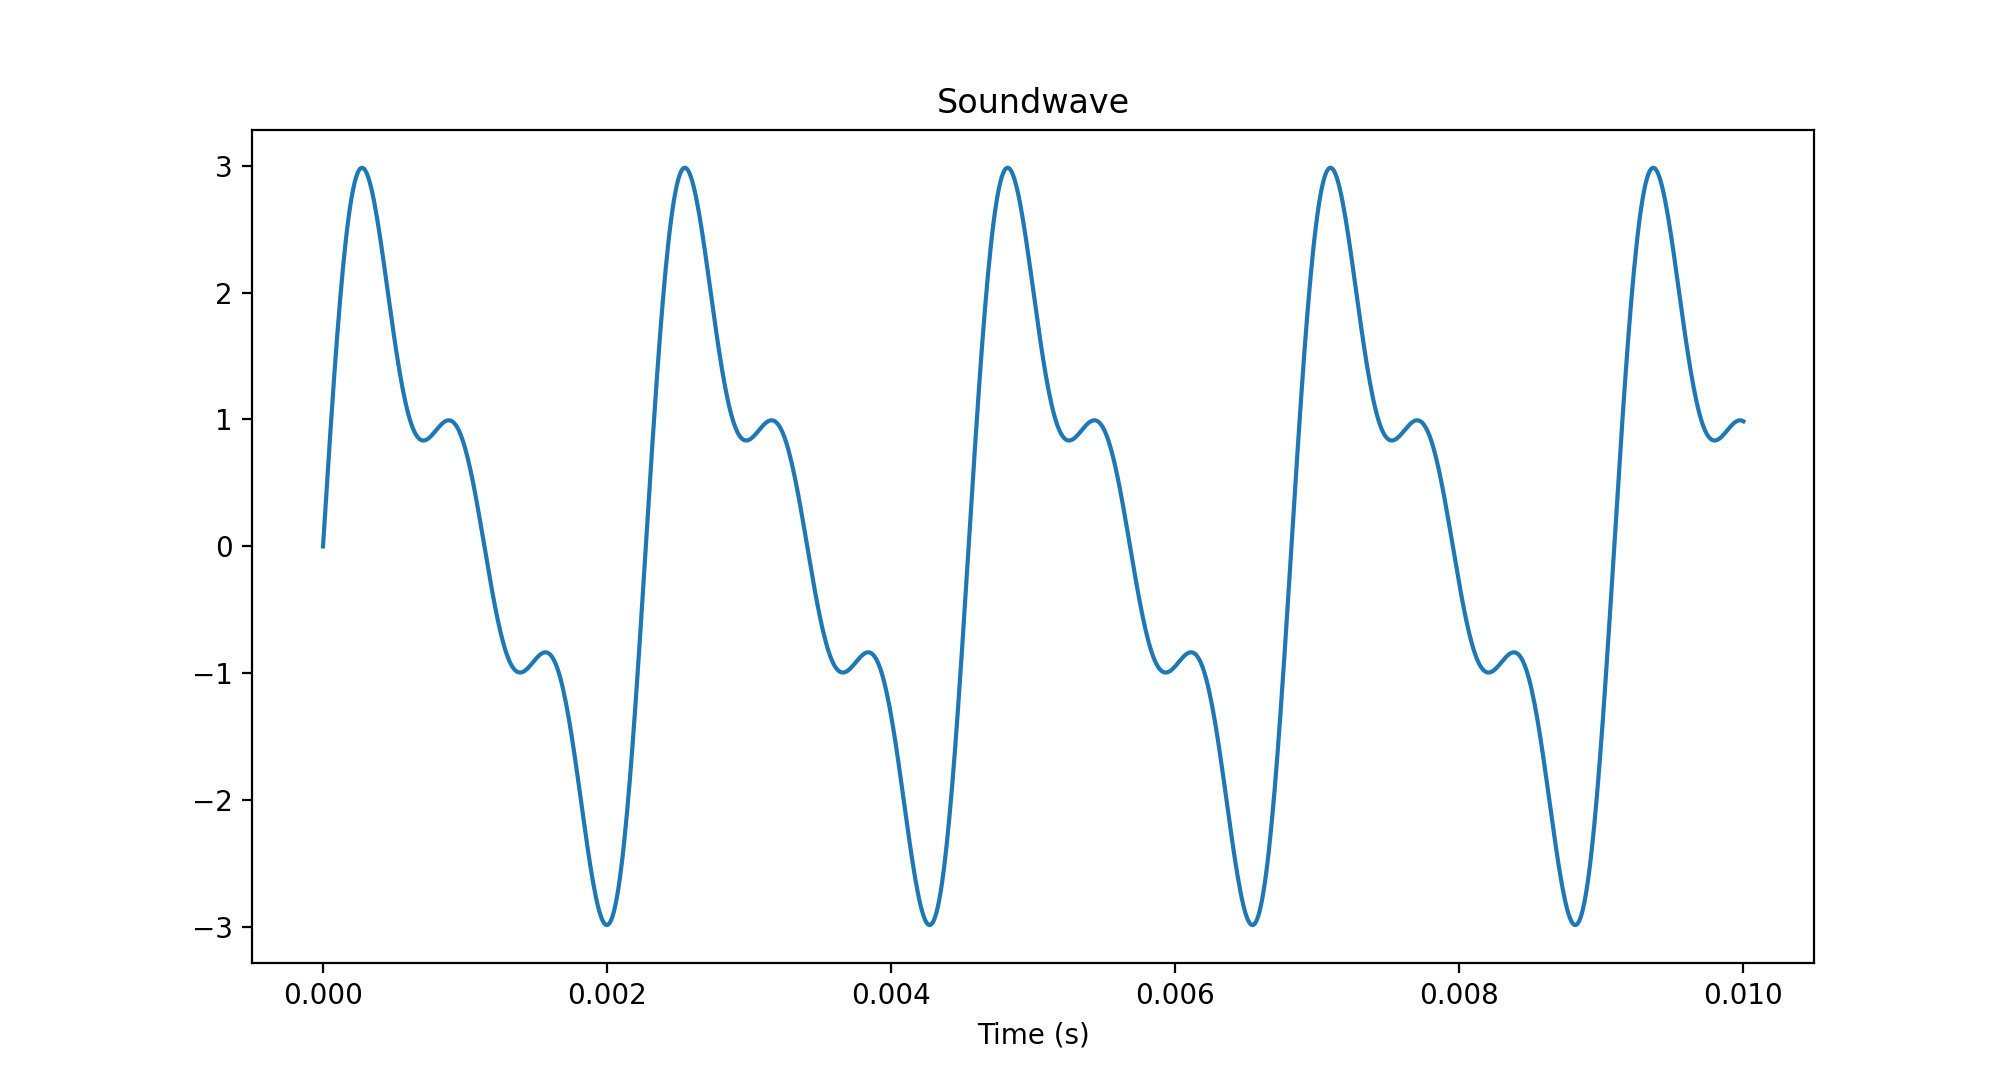
\includegraphics[width=0.8\linewidth]{soundwave.png}

If the guitar string is made tighter (by the tuning pegs) or shorter
(by the guitarist's fingers on the strings), the string vibrates more
times per second.  We measure the number of waves per second and we
call it the \newterm{frequency} of the tone. The unit for frequency is
\newterm{Hertz}: cycles per second.

Musicans have given the different frequencies names. If the guitarist
plucks the lowest note on his guitar, it will vibrate at 82.4
Hertz. The guitarist will say ``That pitch is low E.'' If the string is made
half as long (by a finger on the 12th fret), the frequency will be
twice as fast (164.8 Hertz), and the guitarist will say ``That is E an
octave up.''

For any note, the note that has twice the frequency is one octave
up. The note that has half the frequency is one octave down.

The octave is a very big jump in pitch, so musicians break it up into
12 smaller steps. If the guitarist shortens the E string by one fret,
the frequency will be $82.4 \times 1.059463 \approx 87.3$ Hertz. 

Shortening the string one fret always increases the frequency by a factor of 1.059463. Why?

Because $1.059463^12 = 2$. That is, if you take 12 of these hops, you
end up an octave higher.

This, the smallest hop in western music, is referred to as \newterm{half step}.

\begin{Exercise}[title={Notes and frequecies}, label=note_to_frequency]

The note A near the middle of the piano, is 440Hz. The note E is 7 half steps above A.  What is its frequency?
 
\end{Exercise}
\begin{Answer}[ref=note_to_frequency]

  A is 440 Hz.  Each half-step is a multiplication by $\sqrt[12]{2} = 1.059463094359295$
  So the frequency of E is $(440)(2^{7/12}) = 659.255113825739859$

\end{Answer}


\section{Chords and harmonics}

Of course, a guitarist seldom plays only one string at a
time. Instead, he uses the frets to pick a pitch for each string and
strums all six strings.

Some combinations of frequencies sound better than others. We have
already talked about the octave: if one string vibrates twice for each
vibration of another, they sound sweet together.

Musicians speak of ``the fifth''.  If one string vibrates three times
and the other vibrates twice in the same amount of time, they sound
sweet together.

If one string vibrates 4 times while the other vibrates 3 times, they
sound sweet together. Musicians call this ``the third.''

Each of these different frequencies tickle different cilia in the
inner ear, so you are able to hear all six notes at the same time when
the guitarist strums his guitar.

When a string vibrates, it doesn't create a single sine wave. Yes, the
string vibrates from end-to-end and this generates a sine wave at what
we call \newterm{the fundmental frequency}.However, there are also
``standing waves'' on the string. One of these standing waves, is
still at the centerpoint of the string, but everything to the left of
the centerpoint is going up when everything to the right is going
down. This creates \newterm{an overtone} that is twice the frequency
of the fundamental.

\begin{tikzpicture}[
tl/.style = {% tick labels
    fill=white, inner sep=1pt, font=\scriptsize,
            },                        ]

  \draw[dashed,draw=black,
      domain=-0:6.283,samples=300,variable=\x] 
      plot (\x,{0.7 * sin(deg{\x}/2)});
  \draw[thick,draw=black,
      domain=0:6.283,samples=300,variable=\x] 
  plot (\x,{0.7 * sin(deg{-1 * \x}/2)});
  
  \draw[dashed,draw=black,
      domain=-0:6.283,samples=300,variable=\x] 
      plot (\x,{0.2 * sin(deg{\x})});
  \draw[thick,draw=black,
      domain=0:6.283,samples=300,variable=\x] 
      plot (\x,{0.2 * sin(deg{-1 * \x})});

 \filldraw[black] (0, 0)  circle(3pt);
 \filldraw[black] (6.283, 0)  circle(3pt);

\end{tikzpicture}

The next overtone has two still points -- it divides the string into
three parts.  The outer parts are up while the inner part is
down. It's frequency is three times the fundamental frequency.

\begin{tikzpicture}[
tl/.style = {% tick labels
    fill=white, inner sep=1pt, font=\scriptsize,
            },                        ]

  \draw[dashed,draw=black,
      domain=-0:6.283,samples=300,variable=\x] 
      plot (\x,{0.7 * sin(deg{\x}/2)});
  \draw[thick,draw=black,
      domain=0:6.283,samples=300,variable=\x] 
  plot (\x,{0.7 * sin(deg{-1 * \x}/2)});
  
  \draw[dashed,draw=black,
      domain=-0:6.283,samples=300,variable=\x] 
      plot (\x,{0.2 * sin(1.5 * deg{\x})});
  \draw[thick,draw=black,
      domain=0:6.283,samples=300,variable=\x] 
      plot (\x,{0.2 * sin(1.5 * deg{-1 * \x})});

 \filldraw[black] (0, 0)  circle(3pt);
 \filldraw[black] (6.283, 0)  circle(3pt);

\end{tikzpicture}

And so on: 4 times the fundamental, 5 times the fundamental, etc.

In general, tones with a lot of overtones tend to sound bright. Tones
with just the fundamental sound thin.

Humans can generally hear frequencies from 20Hz to 20,000Hz (or
20kHz).  Young people tend to be able to hear very high sounds better
than older people.

Dogs can generally hear sounds in the 65Hz to 45kHz range.

\section{Making waves in Python}

Let's make a sine wave and add some overtones to it.  Create a file \filename{harmonics.py}

\begin{Verbatim}
import matplotlib.pyplot as plt
import math

# Constants: frequency and amplitude
fundamental_freq = 440.0 # A = 440 Hz
fundamental_amp = 2.0

# Up an octave
first_freq = fundamental_freq * 2.0 # Hz
first_amp = fundamental_amp * 0.5

# Up a fifth more
second_freq = fundamental_freq * 3.0 # Hz
second_amp = fundamental_amp * 0.4

# How much time to show
max_time = 0.0092 # seconds

# Calculate the values 10,000 times per second
time_step = 0.00001 # seconds

# Initialize 
time = 0.0
times = []
totals = []
fundamentals = []
firsts = []
seconds = []

while time <= max_time:
    # Store the time
    times.append(time)
    
    # Compute value each harmonic
    fundamental = fundamental_amp * math.sin(2.0 * math.pi * fundamental_freq * time)
    first = first_amp * math.sin(2.0 * math.pi * first_freq * time)
    second = second_amp * math.sin(2.0 * math.pi * second_freq * time)

    # Sum them up
    total = fundamental + first + second

    # Store the values
    fundamentals.append(fundamental)
    firsts.append(first)
    seconds.append(second)
    totals.append(total)

    # Increment time
    time += time_step

# Plot the data
fig, ax = plt.subplots(2, 1)

# Show each component
ax[0].plot(times, fundamentals)
ax[0].plot(times, firsts)
ax[0].plot(times, seconds)
ax[0].legend()

# Show the totals
ax[1].plot(times, totals)
ax[1].set_xlabel("Time (s)")

plt.show()
\end{Verbatim}

When you run it, you should see a plot of all three sine waves and another plot of their sum:

\includegraphics[width=0.9\linewidth]{harmonicspy.png}

\subsection{Making a sound file}

The graph is pretty to look at, but make a file that we can listen to.

The WAV audio file format is supported on pretty much any device, and
a library for writing WAV files comes with Python.  Lets write some
sine waves and some noise into a WAV file.

Create a file called \filename{soundmaker.py}

\begin{Verbatim}
import wave
import math
import random

# Constants
frame_rate = 16000 # samples per second
duration_per = 0.3 # seconds per sound
frequencies = [220, 440, 880, 392] # Hz
amplitudes = [20, 125]
baseline = 127 # Values will be between 0 and 255, so 127 is the baseline
samples_per = int(frame_rate * duration_per) # number of samples per sound

# Open a file
wave_writer = wave.open('sound.wav', 'wb')

# Not stereo, just one channel
wave_writer.setnchannels(1)

# 1 byte audio means everything is in the range 0 to 255
wave_writer.setsampwidth(1)

# Set the frame rate
wave_writer.setframerate(frame_rate)

# Loop over the amplitudes and frequencies
for amplitude in amplitudes:
    for frequency in frequencies:
        time = 0.0
        # Write a sine wave
        for sample in range(samples_per):
            s = baseline + int(amplitude * math.sin(2.0 * math.pi * frequency * time))
            wave_writer.writeframes(bytes([s]))
            time += 1.0 / frame_rate
            
        # Write some noise after each sine wave
        for sample in range(samples_per):
            s = baseline + random.randint(0, 15)
            wave_writer.writeframes(bytes([s]))
            
# Close the file
wave_writer.close()
\end{Verbatim}

When you run it, it should create a sound file with several tones of
different frequencies and volumes. Each tone should be followed by
some noise.

\chapter{Alternating Current}

We have discussed the voltage and current created by a battery.  A
battery pushes the electrons in one direction at a constant voltage;
this is known as \newterm{Direct Current} or DC. A battery typically
provides between 1.5 and 9 volts.

The electrical power that comes into your home on wires is
different. If you plotted the voltage over time, it would look like
this:

\begin{tikzpicture}[
tl/.style = {% tick labels fill=white, inner sep=1pt,
  font=\scriptsize, }, ]
% grid
\draw[sdkblue, very thin, xstep=0.5235, ystep=0.425] (0,-1.85) grid
(6.6,1.85);

% y tick label
\foreach \y in {-170, -85, 85, 170}{\node[tl,left=1mm] at (0,{\y/100})
  {$\y$};}

% x tick label
\foreach \x in {0.004,0.008, 0.012, 0.016}{\node[tl,below=1mm] at
  ({392.67*\x},0) {$\x$};}

% axes
\draw[->,thick] (0,0) -- (6.5,0) node[right] {$seconds$};
\draw[->,thick] (0,-1.8) -- (0, 1.8) node[above] {$volts$};
% curve
\draw[<->,thick,draw=black,domain=0:6.5,samples=300,variable=\x] plot
(\x,{sin(deg(\x)) * 1.7});
\end{tikzpicture}

The $x$ axis here represents ground. When you insert a two-prong plug
into an outlet, one is ``hot'' and the other is ``ground''. Ground
represents 0 volts and should be the same voltage as the dirt under
the building.

The voltage is a sine wave at 60Hz. Your voltage fluctuates between
-170v and 170v. Think for a second what that means: The power company
pushes electrons at 170v and then pulls electrons at 170v.  It
alternates back and forth this way 60 times per second.

\section{Power of AC}

Let's say you turn on your toaster which has a resistance of 14.4
ohms. How much energy (in watts) does it change from electrical energy
to heat?  We know that $I = V/R$ and we know that watts of power is
$IV$. So given a voltage of $V$, the toaster is consuming $V^2/R$
watts.

However, $V$ is fluctuating. Let's plot the power the toaster is consuming:

\begin{tikzpicture}[
tl/.style = {% tick labels
    fill=white, inner sep=1pt, font=\scriptsize,
            },                        ]
% grid
\draw[sdkblue, very thin, xstep=0.5235, ystep=0.5] (0,0) grid (6.6,2.1);

% y tick label
\foreach \y in {500, 1000, 1500, 2000}{\node[tl,left=1mm] at (0,{\y/1000}) {$\y$};}

% x tick label
\foreach \x in {0.004,0.008, 0.012, 0.016}{\node[tl,below=1mm] at ({392.67*\x},0) {$\x$};}

% axes
\draw[->,thick] (0,0) -- (6.5,0) node[right] {$seconds$};
\draw[->,thick] (0,0) -- (0, 2.1) node[above] {$watts$};
% curve
\draw[<->,thick,draw=black,domain=0:6.5,samples=300,variable=\x]
      plot (\x,{sin(deg(\x))^2 * 2.007});
\end{tikzpicture}

Another sine wave! Here is a lesser-known trig identity: $\left( \sin(x) \right)^2 = \frac{1}{2} - \frac{1}{2}\cos(2x)$

So this is actually a cosine wave flipped upside down, scaled down by
half the peak power and translated up so that it is never
negative. Note that it is also twice the frequency of the voltage sine
wave.

If we say the peak voltage is $V_p$ and the resistance of the toaster
is $R$, the power is given by

$$\frac{V_p^2}{2R} - \frac{V_p^2}{2R} \cos \left(\frac{2\pi t}{120} \right)$$

As a toaster user and as someone who pays a power bill, you are mostly
interested in the average power.  To get the average power, you take
the area under the power graph and divide it by the amount of time.

We can think of the area under the curve as two easy-to-integrate quantites summed:
\begin{itemize}
\item A constant function of $y = frac{V_p^2}{2R}$
\item A wave $y = - \frac{V_p^2}{2R} \cos \left(\frac{2\pi t}{120} \right)$
\end{itemize}

\begin{tikzpicture}[
tl/.style = {% tick labels
    fill=white, inner sep=1pt, font=\scriptsize,
            },                        ]
% grid
\draw[sdkblue, very thin, xstep=0.5235, ystep=0.5] (0,-1.1) grid (6.6,1.1);

% y tick label
\foreach \y in {-1000, -500, 500, 1000}{\node[tl,left=1mm] at (0,{\y/1000}) {$\y$};}

% x tick label
\foreach \x in {0.004,0.008, 0.012, 0.016}{\node[tl,below=1mm] at ({392.67*\x},0) {$\x$};}

% axes
\draw[->,thick] (0,0) -- (6.5,0) node[right] {$seconds$};
\draw[<->,thick] (0,-1.1) -- (0, 1.1) node[above] {$watts$};
% curve
\draw[<->,thick,draw=black] (0,1.003) -- (6.5, 1.003) node[right] {Constant: $\frac{V_p^2}{2R}$};
\draw[<->,thick,draw=black,domain=0:6.5,samples=300,variable=\x]
      plot (\x,{-1 * cos(deg(\x) * 2) * 1.003}) node[right]{Wave:$- \frac{V_p^2}{2R} \cos \left(\frac{2\pi t}{120} \right)$};
\end{tikzpicture}
    
When we integrate that constant function we get $\frac{t V_p^2}{2R}$

When we integrate that wave for a complete cycle we get...zero! The
positive side of the wave is canceled out by the negative side.

So, the average power is $\frac{V_p^2}{2R}$ watts.

Someone at some point said ``I'm used to power being $V^2/R$. Can
we define a voltage measure for AC power such that this is always true?''

So we started using $V_{rms}$ which is just
$\frac{V_p}{\sqrt{2}}$. If you look on the back of anything that plugs
into a standard US power outlet, it will say something like ``For
120v''.  What they mean is ``For 120v RMS, so we expect the voltage to
fluctuate back and forth from 170v to -170v.''

Notice that this is the same Root-Mean-Squared that we defined
earlier, but now we know that if $y = \sin(x)$, the RMS of $y$ is
$1/\sqrt{2} \approx 0.707$.

For current, we do the same thing: If the current is AC, the power
consumed by a resistor is $I_{RMS}^2 R$, where $I_{RMS}$ is the peak
current divided by $sqrt{2}$.

\section{Power Line Losses}

A wire has some resistance. Thinner wires tend to have more resistance
than thicker ones. Aluminum wires tend to have more resistance than
copper wires.

Let's say that the power that comes to your house has to travel 20 km
from the generator in a cable that has about $1 \Omega$ of resistance
per km.  Let's say that your home is consuming 12 kilowatts of power.

If that power is 120v RMS from the generator to your home, what
percentage of the power is lost heating the power line? 10 amps RMS
flow through your home. When that current goes through the wire, $I^2
R = (100)(20) = 2000 watts$ is lost to heat.

So the power company would need to supply 14 kilowatts of power,
knowing that 2 kilowatts would be lost on the wires.

What if the power company moved the power at 120,000 volts RMS? Now
only 0.01 amps RMS flow through your home. When that current goes
through the wire $I^2R = (0.0001)(20) = .002$ watts of power are lost
on the power lines.

It is much, much more efficent. The only problem is that 120,000 volts
would be incredibly dangerous.  So the power company moves power long
distances at very high voltages, like 765 kV.  Before the power is
brought into your home, it is converted into a lower voltage using a
\newterm{transformer}.

\section{Transformers}

A transformer is a device that converts electrical power from one
voltage to another. A good tranformer is more than 95\% efficient. The
details of magnetic fields, flux, and inductance are beyond this scope
of this chapter, so I am going to give a relatively simple explanation
and admit that it is incomplete.

A transformer is a ring with two sets of coils wrapped around it.

\includegraphics[width=0.5\textwidth]{transformer.png}

(Diagram from Wikipedia)

When AC current is run through the primary winding, it create magnetic
flux in the ring.  The magnetic flux induces current in the secondary
winding.

If $V_P$ is the voltage across the primary winding and $V_S$ is the
voltage across the secondary winding, they are related by the
following equation:

$$\frac{V_P}{V_S} = \frac{N_P}{N_S}$$

where $N_P$ and $N_S$ are the number of turns in the primary and
secondary windings.

There are usually at least two transformers between you and the very
high voltage lines.  There are tranformers at the substation that make
the voltage low enough to travel on regular utility poles. On the
utility poles, you will see cans that contain smaller
transformers. Those step the voltage down to make the power safe to
enter your home.

\section{Phase and 3-phase power}

If two waves that are ``in sync'' we say they have the same \newterm{phase}.

\begin{tikzpicture}[
tl/.style = {% tick labels fill=white, inner sep=1pt,
  font=\scriptsize, }, ]
% grid
\draw[sdkblue, very thin, xstep=0.5235, ystep=0.425] (0,-1.85) grid
(13,1.85);

% axes
\draw[->,thick] (0,0) -- (13,0);
% curve
\draw[thick,draw=black,domain=0:13,samples=500,variable=\x] plot
(\x,{sin(deg(\x)) * 1.7});
\draw[thick,dashed, draw=black,domain=0:13,samples=500,variable=\x] plot
(\x,{sin(deg(\x)) * 0.9});
\end{tikzpicture}

If they are the same frequency, but are not in-sync, we can talk about
the difference in their phase.

\begin{tikzpicture}[
tl/.style = {% tick labels fill=white, inner sep=1pt,
  font=\scriptsize, }, ]
% grid
\draw[sdkblue, very thin, xstep=0.5235, ystep=0.425] (0,-1.85) grid
(13,1.85);

% axes
\draw[->,thick] (0,0) -- (13,0);
% curve
\draw[thick,draw=black,domain=0:13,samples=500,variable=\x] plot
(\x,{sin(deg(\x)) * 1.7});
\draw[thick,dashed, draw=black,domain=0:13,samples=500,variable=\x] plot
(\x,{sin(deg(\x) - 90) * 0.9});
\end{tikzpicture}

Here we see that the smaller wave is lagging by $\pi/2$ or $90^\circ$.

In most power grids, there are usually 3 wires carrying the power.
The voltage on each is $2\pi/3$ out of phase with the other two:

\begin{tikzpicture}[
tl/.style = {% tick labels fill=white, inner sep=1pt,
  font=\scriptsize, }, ]
% grid
\draw[sdkblue, very thin, xstep=0.5235, ystep=0.425] (0,-1.85) grid
(13,1.85);

% axes
\draw[->,thick] (0,0) -- (13,0);
% curve
\draw[thick,draw=black,domain=0:13,samples=500,variable=\x] plot
(\x,{sin(deg(\x)) * 1.7});
\draw[thick,dashed, draw=black,domain=0:13,samples=500,variable=\x] plot
(\x,{sin(deg(\x) - 120) * 1.7});
\draw[thick,draw=sdkblue,domain=0:13,samples=500,variable=\x] plot
(\x,{sin(deg(\x) + 120) * 1.7});
\end{tikzpicture}

This is nice in two ways:
\begin{itemize}
\item While the power in each wire is fluctuating, the total power is not fluctuating at all.
\item While the power plant is pushing and pulling electrons on each
  wire, the total number number of electrons leaving the load is zero.
\end{itemize}
(Both these assume that there each wire is attached to a load with the same constant resistance.)

In big industrial factories, you will see all three wires enter the
building. Large amounts of smooth power delivery means a lot to an
industrial user.

In residential settings, each home gets its power from one of the three
wires. However two wires typically carry power into the home. Each
one carries 120V RMS, but they are out of phase by 180 degree. Lights
and small appliances are connected to one of the wires and ground, so
they get 120V RMS.  Large appliances, like air conditioners and
washing machines, are connected across the two wires so they get 240V
RMS.

\begin{tikzpicture}[
tl/.style = {% tick labels fill=white, inner sep=1pt,
  font=\scriptsize, }, ]
% grid
\draw[sdkblue, very thin, xstep=0.5235, ystep=0.425] (0,-1.85) grid
(13,1.85);

% axes
\draw[->,thick] (0,0) -- (13,0);
% curve
\draw[thick,draw=black,domain=0:13,samples=500,variable=\x] plot
(\x,{sin(deg(\x)) * 1.7});
\draw[thick,dashed, draw=black,domain=0:13,samples=500,variable=\x] plot
(\x,{sin(deg(\x) + 180) * 1.7});
\draw[<->, thick, draw=black] (7.85398, 0) -- (7.85398, 1.7) node [midway, right] {120V};
\draw[<->, thick, draw=black] (4.712, -1.7) -- (4.712, 1.7);
\draw (4.712, 0.8) node[right] {240V};
\end{tikzpicture}


How do you get two circuits, 180 degrees out of phase, from one
circuit?  Using a center-tap transformer.

FIXME: Diagram here





\graphicspath{{../../Modules/Polynomials/}}
\chapter{Introduction to Polynomials}

Watch Khan Academy's \textbf{Polynomials intro} video at \url{https://www.khanacademy.org/math/algebra2/x2ec2f6f830c9fb89:poly-arithmetic/x2ec2f6f830c9fb89:poly-intro/v/polynomials-intro}

A \emph{monomial}\index{monomial} is the product of a number and a variable raised to a non-negative power. Here are some monomials:
\begin{multicols}{4}
  \begin{equation*}
    3 x^2
  \end{equation*}
  \begin{equation*}
    -2 x^{15}
  \end{equation*}

  \begin{equation*}
    \pi x^2
  \end{equation*}
  \begin{equation*}
    (3.33)x^{100}
  \end{equation*}

  \begin{equation*}
    7x
  \end{equation*}
  \begin{equation*}
    3
  \end{equation*}

  \begin{equation*}
    -\frac{2}{3}x^{12}
  \end{equation*}
  \begin{equation*}
    0
  \end{equation*}

  
\end{multicols}

The exponent is called the \emph{degree} of the monomial\index{monomial!degree}. Examples: $3x^{17}$
has degree 17, $-7x$ has degree 1, and $3.2$ has degree 0 (because you can think of it as $(3.2)x^0$).

The number in the product is called the \emph{coefficient}\index{monomial!coefficient}.  Example: $3x^{17}$ has a coefficient of 3, $-2x$ has a coefficient of -2, and $(3.4)x^{1000}$ has a coefficient of 3.4.

A polynomial \index{polynomial!definition of} is the sum of one or more monomials.  Here are some polynomials:
\begin{multicols}{3}
  \begin{equation*}
    4 x^2 + 9x + 3.9
  \end{equation*}
  \begin{equation*}
    -2 x^{10} + (3.4)x - 45x^{900} - 1
  \end{equation*}
  \begin{equation*}
    \pi x^2 + \pi x + \pi
  \end{equation*}
  \begin{equation*}
    3.3
  \end{equation*}
  \begin{equation*}
   7x + 2
  \end{equation*}
  \begin{equation*}
    3x^{20}
  \end{equation*}
\end{multicols}
We say that each monomial is a \emph{term} of the polynomial.

$x^{-5} + 12$ is \emph{not} a polynomial because the first term has a negative exponent.

$x^{2} - 32x^{\frac{1}{2}} + x$ is \emph{not} a polynomial because the second term has a non-integer exponent.

$\frac{x + 2}{x^2 + x + 5}$ is \emph{not} a polynomial because it is not just a sum of monomials.
\clearpage

\begin{Exercise}[title={Identifying Polynomials}, label=findpolynomials]
    Circle only the polynomials
\begin{multicols}{3}
  \begin{equation*}
    -2 x^3 + \frac{1}{2}x + 3.9
  \end{equation*}
  \begin{equation*}
    2 x^{-10} + 4x - 1
  \end{equation*}
  
  \begin{equation*}
    (4.5)x^2 + \pi x
  \end{equation*}
  \begin{equation*}
    x^{\frac{2}{3}}
  \end{equation*}
  
  \begin{equation*}
   7
  \end{equation*}
  \begin{equation*}
    3x^{20} + 2x^{19} -5 x^{18}
  \end{equation*}
\end{multicols}
\end{Exercise}

\begin{Answer}[ref=findpolynomials]
\begin{multicols}{3}
  \begin{equation*}
    \boxed{-2 x^3 + \frac{1}{2}x + 3.9}
  \end{equation*}
  \begin{equation*}
    2 x^{-10} + 4x - 1
  \end{equation*}

  \begin{equation*}
    \boxed{(4.5)x^2 + \pi x}
  \end{equation*}
  \begin{equation*}
    x^{\frac{2}{3}}
  \end{equation*}

  \begin{equation*}
   \boxed{7}
  \end{equation*}
  \begin{equation*}
    \boxed{3x^{20} + 2x^{19} -5 x^{18}}
  \end{equation*}
\end{multicols}

\end{Answer}

\chapter{Python Lists}

Watch CS Dojo's \textbf{Introduction to Lists in Python} video at \url{https://www.youtube.com/watch?v=tw7ror9x32s}

To review, Python list is an indexed collection. The indices start at
zero. You can create a list using square brackets.

Now you are going to write a program that makes an array of
strings. Type this code into a file called \url{faves.py}:

\begin{Verbatim}
favorites = ["Raindrops", "Whiskers", "Kettles", "Mittens"]
favorites.append("Packages")
print("Here are all my favorites:", favorites)
print("My most favorite thing is", favorites[0])
print("My second most favorite is", favorites[1])
number_of_faves = len(favorites)
print("Number of things I like:", number_of_faves)

for i in range(number_of_faves):
    print(i, ": I like", favorites[i])
\end{Verbatim}

Run it:
\begin{Verbatim}[commandchars=\\\{\}]
$ \textbf{python3 faves.py}
Here are all my favorites: ['Raindrops', 'Whiskers', 'Kettles', 'Mittens', 'Packages']
My most favorite thing is Raindrops
My second most favorite is Whiskers
Number of things I like: 5
0 : I like Raindrops
1 : I like Whiskers
2 : I like Kettles
3 : I like Mittens
4 : I like Packages
\end{Verbatim}
After you have run the code, study it until the output makes sense.

\begin{Exercise}[title={Assign into list}, label=assignintolist]
  Before you list the items, replace "Mittens" with "Gloves".
\end{Exercise}
\begin{Answer}[ref=assignintolist]
\begin{Verbatim}
favorites[3] = "Gloves"
\end{Verbatim}
\end{Answer}

\section{Evaluating Polynomials in Python}

First, before you go any further, you need to know that raising a
number to a power is done with ** in Python.  So for example, to get
$5^2$, you would write \texttt{5**2}.

Back to polynomials: if you had a polynomial like $2x^3 -9x + 12$, you
could write it like this: $12x^0 + (-9)x^1 + 0x^2 + 2x^3$.  We could
use this representation to keep a polynomial in a Python list. We
would simply store all the coefficients in order:
\begin{Verbatim}
pn1 = [12,-9,0,2]
\end{Verbatim}

In the list, the index of each coefficient would correspond to the
degree of that monomial. For example, in the list 2 is at index 3, so
that entry represents $2x^3$.

In the last chapter, you evaluated the polynomial $x^3 - 3x^2 + 10x -
12$ at $x=4$. Now you will write code that does that evalution.
Create a file called \url{polynomials.py} and type in the following:

\begin{Verbatim}
def evaluate_polynomial(pn, x):
    sum = 0.0  
    for degree in range(len(pn)):
        coefficient = pn[degree]
        term_value = coefficient * x ** degree
        sum = sum + term_value
    return sum
   
pn1 = [-12.0, 10.0, -3.0, 1.0]
y = evaluate_polynomial(pn1, 4.0)
print("Polynomial 1: When x is 4.0, y is", y)
\end{Verbatim}

Run it. It should evaluate to 44.0.

\begin{Exercise}[title={Evaluate Polynomials}, label=pyevalpolynomials]
Using the function that you just wrote, add a few lines of code to \url{polynomials.py} to evaluate the following polynomials:
\begin{itemize}
\item Find $4x^4 - 7x^3 - 2x^2 + 5x + 2.5$ at $x = 8.5$.  It should be 16481.875
\item Find $5x^5 - 9$ at $x = 2.0$.  It should be 151.0
\end{itemize}
\end{Exercise}
\begin{Answer}[ref=pyevalpolynomials]
\begin{Verbatim}
pn2 = [2.5, 5.0, -2.0, -7.0, 4.0]
y = evaluate_polynomial(pn2, 8.5)
print("Polynomia 2: When x is 8.5, y is", y)

pn3 = [-9.0, 0.0, 0.0, 0.0, 0.0, 5.0]
y = evaluate_polynomial(pn3, 2.0)
print("Polynomial 3: When x is 2.0, y is", y)    
\end{Verbatim} 
\end{Answer}

\section{Plot the polynomial}

We can evaluate a polynomial at many points and plot them on a
graph. You are going to write the code to do this.  Create a new file
called \url{plot_polynomial.py}. Copy your \pyfunction{evaluate\_polynomial}
function into the new file.

Add a line at the beginning of the program that imports the plotting library matplotlib:
\begin{Verbatim}
import matplotlib.pyplot as plt
\end{Verbatim}

After the \pyfunction{evaluate\_polynomial} function:
\begin{itemize}
\item Create a list with polynomial coefficients.
\item Create two empty arrays, one for x values and one for y values.
\item Fill the x array with values from -3.5 to 3.5. Evaluate the polynomial at each of these points; put those values
  in the y array.
\item Plot them
\end{itemize}

Like this:
\begin{Verbatim}
# x**3 - 7x + 6
pn = [6.0, -7.0, 0.0, 1.0]

# These lists will hold our x and y values
x_list = []
y_list = []

# Start at x=-3.5
current_x =-3.5

# End at x=3.5
while current_x <= 3.5:
    current_y = evaluate_polynomial(pn, current_x)

    # Add x and y to respective lists
    x_list.append(current_x)
    y_list.append(current_y)

    # Move x forward
    current_x += 0.1

# Plot the curve
plt.plot(x_list, y_list)
plt.grid(True)
plt.show()
\end{Verbatim}

You should get a beautiful plot like this:

\includegraphics[width=\textwidth]{polyplot1.png}

If you received an error that the matplotlib was not found, use pip to install it:
\begin{Verbatim}[commandchars=\\\{\}]
$ \textbf{pip install matplotlib}
\end{Verbatim}

\chapter{Adding and Subtracting Polynomials}

Watch Khan Academy's \textbf{Adding polynomias} video at \url{https://youtu.be/ahdKdxsTj8E}

When adding two monomials of the same degree, you sum their coefficients:
\begin{equation*}
  7x^3 + 4x^3 = 11x^3
\end{equation*}\index{adding!monomials}

Using this idea, when adding two polynomials, you convert it into one long
polynomial and then simplify by combining terms with the same degree. For example:
\begin{multline*}
  (10x^3 - 2x + 13) + (-5x^2 + 7x -12) \\
  = 10x^3 + (-2)x + 13 + (-5)x^2 + 7x + (-12) \\
  = 10x^3 + (-5)x^2 + (-2 + 7)x + (13 - 12) \\
  = 10x^3 - 5x^2 + 5x + 1
\end{multline*}\index{adding!polynomials}

\begin{Exercise}[title=Adding Polynomials Practice, label=addpns]
  Add the following polynomials:
  \Question{$2x^3 - 5x^2 + 3x - 9$ and $x^3 - 2x^2 - 2x - 9$}
  \vspace{20mm}
  \Question{$3x^5 - 5x^3 + 3x^2 - x - 3$ and $2x^4 - 2x^3 - 2x^2 + x - 9$}
  \vspace{20mm}
\end{Exercise}
\begin{Answer}[ref=addpns]$3x^3 - 7x^2 + x - 18$ and $3x^5 - 7x^3 + x^2 - 12$\end{Answer}

Notice that in the second question, the degree 1 term disappears completely: $(-x) + x = 0$

One more tricky thing that can happen: Sometimes the coefficients don't add nicely.  For example:
\begin{equation*}
  \pi x^2 - 3 x^2 = (\pi - 3) x^2
\end{equation*}
That is as far as you can simplify it.
    
\section{Subtraction}

Now watch Khan Academy's \textbf{Subtracting polynomials} at \url{https://youtu.be/5ZdxnFspyP8}.

When subtracting one polynomial from the other, it is a lot like
adding two polynomials. The difference: when make the two polynomials
into one long polynomial, we multiply each monomial that is being
subtracted by -1. For example:
\begin{multline*}
  (2x^2 - 3x + 9) - (5x^2 - 7x + 4) \\
  = 2x^2 + (-3)x + 9 + (-5)x^2 + 7x + (-4) \\
  = (2 - 5)x^2 + (-3 + 7)x + (9-4) \\
  = -3x^2 + 4x + 5
\end{multline*}

\begin{Exercise}[title=Subtracting Polynomials Practice, label=subtractpns]
  Add the following polynomials:
  \Question{$(2x^3 - 5x^2 + 3x - 9) - (x^3 - 2x^2 - 2x - 9)$}
  \vspace{20mm}
  \Question{$(3x^5 - 5x^3 + 3x^2 - x - 3) - (2x^4 - 2x^3 - 2x^2 + x - 9)$}
  \vspace{20mm}
\end{Exercise}
\begin{Answer}[ref=subtractpns]$x^3 - 3x^2 + 5x$ and $x^5 - 3x^3 + 5x^2 - 2x + 6$\end{Answer}

\section{Adding Polynomials in Python}

As a reminder, in our Python code, we are representing a polynomial
with a list of coefficients.  The first coefficient is the constant
term. The last coefficient is the leading coefficient. So, we can
imagine $-5x^3 + 3x^2 - 4x + 9$ and $2x^3 +4x^2 - 9$ would look
like this: \textit{FIXME: Diagram here}

To add the two polynomials then, we sum the coefficients for each degree.
\textit{FIXME: Diagram here}

Create a file called \filename{add\_polynomials.py}, and type in the following: 
\begin{Verbatim}
def add_polynomials(a, b):
    degree_of_result = len(a)
    result = []
    for i in range(degree_of_result):
        coefficient_a = a[i]
        coefficient_b = b[i]
        result.append(coefficient_a + coefficient_b)
    return result

polynomial1 = [9.0, -4.0, 3.0, -5.0]
polynomial2 = [-9.0, 0.0, 4.0, 2.0]
polynomial3 = add_polynomials(polynomial1, polynomial2)

print('Sum =', polynomial3)
\end{Verbatim}

Run the program.

Unfortunately, this code only works if the polynomails are the same length. For
example, try making \pyvar{polynomial1} have a larger degree than
\pyvar{polynomial2}:
\begin{Verbatim}
# x**4 - 5x**3 + 3x**2 - 4x + 9
polynomial1 = [9.0, -4.0, 3.0, -5.0, 1.0]
  
# 2x**3 + 4x**2 - 9  
polynomial2 = [-9.0, 0.0, 4.0, 2.0]
polynomial3 = add_polynomials(polynomial1, polynomial2)
print('Sum =', polynomial3)
\end{Verbatim}

See the problem?

\begin{Exercise}[title=Dealing with polynomials of different degrees, label=pyaddpolys]
  
Can you fix the function \pyfunction{add\_polynomials} to handle polynomials of different degrees?

Here is a hint: In Python, there is a \pyfunction{max} function that returns the largest of the numbers it is passed.
\begin{Verbatim}
biggest = max(5,7)
\end{Verbatim}
Here \pyvar{biggest} would be set to 7.

Here is another hint: If you have an array \pyvar{mylist}, \pyvar{i},
a non-negative integer, is only a legit index if \texttt{i <
  len(mylist)}.
\end{Exercise}
\begin{Answer}[ref=pyaddpolys]
\begin{Verbatim}
def add_polynomials(a, b):
    degree_of_result = max(len(a), len(b))
    result = []
    for i in range(degree_of_result):
        if i < len(a):
            coefficient_a = a[i]
        else:
            coefficient_a = 0.0   

        if i < len(b):
            coefficient_b = b[i]
        else:
            coefficient_b = 0.0
            
        result.append(coefficient_a + coefficient_b)
    return result
\end{Verbatim}
\end{Answer}

\section{Scalar multiplication of  polynomials}

If you multiply a polynomial with a number, the distributive property applies:
\begin{equation*}
  (3.1)(2x^2 + 3x + 1) = (6.2)x^2 + (9.3)x + 3.1
\end{equation*}
(When we are talking about things that are more complicated than a number, we use the word \emph{scalar} to mean ``Just a number''. So this is the product of a scalar and a polynomial.)

In \filename{add\_polynomials.py}, add a function to that multiplies a scalar and a polynomial:
\begin{Verbatim}
def scalar_polynomial_multiply(s, pn):
    result = []
    for coefficient in pn:
        result.append(s * coefficient)
    return result
\end{Verbatim}

Somewhere near the end of the program, test this function:
\begin{Verbatim}
polynomial4 = scalar_polynomial_multiply(5.0, polynomial1)
print('Scalar product =', polynomial_to_string(polynomial4))
\end{Verbatim}

\begin{Exercise}[title=Subtract polynomials in Python, label=pysubpoly]
Now implement a function that does subtraction using
\pyfunction{scalar\_polynomial\_multiply} and
\pyfunction{add\_polynomials}.

It should look like this:
\begin{Verbatim}
def subtract_polynomial(a, b):
    ...Your code here...

polynomial5 = [9.0, -4.0, 3.0, -5.0]
polynomial6 = [-9.0, 0.0, 4.0, 2.0, 1.0]
polynomial7 = subtract_polynomial(polynomial5, polynomial6)
print('Difference =', polynomial_to_string(polynomial7))
\end{Verbatim}
\end{Exercise}
\begin{Answer}[ref=pysubpoly]
\begin{Verbatim}
def subtract_polynomial(a, b):
    neg_b = scalar_polynomial_multiply(-1.0, b)
    return add_polynomials(a, neg_b)
\end{Verbatim}
\end{Answer}


    

\chapter{Multipying Polynomials}

Watch Khan Academy's \textbf{Multipying monomials} at \url{https://youtu.be/Vm7H0VTlIco}.

To review, when you multiply two monomials, you take the product of
their coefficients and the sum of their degrees:
\begin{equation*}
  (2x^6)(5x^3) = (2)(5)(x^6)(x^3) = 10x^9
\end{equation*}
If you have a product of more than two monomials, multiply \emph{all}
the coefficients and sum \emph{all} the exponents:
\begin{equation*}
  (3x^2)(2x^3)(4x) = (3)(2)(4)(x^2)(x^3)(x^1) = 24x^6
\end{equation*}

\begin{Exercise}[title={Multiplying monomials}, label=multmonomials]
Multiply these monomials
  \Question $(3x^2)(5x^3)$
\vspace{20mm}
  \Question $(2x)(4x^9)$
\vspace{20mm}
  \Question $(-5.5x^2)(2x^3)$
\vspace{20mm}
  \Question $(\pi)(-2x^5)$
\vspace{20mm}
  \Question $(2x)(3x^2)(5x^7)$
\vspace{20mm}
\end{Exercise}
\begin{Answer}[ref=multmonomials]
  $(3x^2)(5x^3) = 15x^5$
  
  $(2x)(4x^9) = 8x^{10}$
  
  $(-5.5x^2)(2x^3) = -11x^5$

  $(\pi)(-2x^5) = -2\pi x^5$
  
  $(2x)(3x^2)(5x^7) = 30x^{10}$
\end{Answer}

\section{Multiplying a monomial and a polynomial}

Watch Khan Academy's \textbf{Multiplying monomials by polynomials} at \url{https://youtu.be/pD2-H15ucNE}.

When multiplying a monomial and a polynomial, you use the the distributive property. Then it is just multiplying several pairs of monomials:
\begin{multline*}
  (3x^2)(4x^3 - 2x^2 + 3x - 7) \\
  = (3x^2)(4x^3) + (3x^2)(-2x^2) + (3x^2)(3x) + (3x^2)(-7) \\
  = 12x^5 - 6x^4 + 9x^3 -21x^2
\end{multline*}

\begin{Exercise}[title={Multiplying a monomial and a polynomial}, label=multmonopoly]
Multiply these monomials
\Question $(3x^2)(5x^3 - 2x + 3)$
\vspace{20mm}
\Question $(2x)(4x^9 - 1)$
\vspace{20mm}
\Question $(-5.5x^2)(2x^3 + 4x^2 + 6)$
\vspace{20mm}
\Question $(\pi)(-2x^5 + 3x^4 + x)$
\vspace{20mm}
\Question $(2x)(3x^2)(5x^7 + 2x)$
\end{Exercise}
\begin{Answer}[ref=multmonopoly]
  $(3x^2)(5x^3 - 2x + 3) = 15x^6 - 6x^3 + 6x^2$

  $(2x)(4x^9 - 1) = 8x^{10} - 2x$

  $(-5.5x^2)(2x^3 + 4x^2 + 6) = 11x^5 - 22x^4 + 33x^2$

  $(\pi)(-2x^5 + 3x^4 + x) = -2\pi x^5 + 3\pi x^4 + \pi x$

  $(2x)(3x^2)(5x^7 + 2x) = 30x^{10} + 12x^4$
\end{Answer}

\section{Multiplying polynomials}

Watch Khan Academy's \textbf{Multiplying binomials by polynomials} video at \url{https://youtu.be/D6mivA_8L8U}

When you are multiplying two polynomials, you will use the
distributive property several times to make it one long
polynomial. Then you will combine the terms with the same degree. For
example,
\begin{multline*}
  (2x^2 - 3)(5x^2 + 2x - 7) \\
  =   (2x^2)(5x^2 + 2x - 7) + (-3)(5x^2 + 2x - 7) \\
  =   (2x^2)(5x^2) + (2x^2)(2x) + (2x^2)(-7) + (-3)(5x^2) + (-3)(2x) + (-3)(-7) \\
  =   10^4 + 4x^3 + -14x^2 + -15x^2 + -6x + 21
  =   10^4 + 4x^3 + -29x^2 + -6x + 21
\end{multline*}

One common form that you will see is multiplying two binomials together:
\begin{multline*}
(2x + 7)(5x + 3) = (2x)(5x + 3) + (7)(5x+3) = (2x)(5x) + (7)(5x) + (2x)(3) + (7)(3)
\end{multline*}
Notice the product has become the sum of four parts: the firsts, the
inners, the outers, and the lasts. People sometimes use the mnemonic
FOIL to remember this pattern, but there is a general rule that works
for all product of polynomials, not just binomials.  Here it is: Every
term in the first will be multiplied by every term in the second, and
then just add them together.

So, for example, if you have a polynomial $s$ with three terms and you
multiply it by a polynomial $t$ with five terms, you will get a sum of
15 terms -- each term is a product of two monomials, one from $s$ and
one from $t$.  (Of course, several of those terms might have the same
degree, so they will be combined together when you simplify. Thus you
typically end up with a polynomial with less than 15 terms.)

Using this rule, here is how I would multiply $2x^2 - 3x + 1$ and
$5x^2 + 2x - 7$:
\begin{multline*}
  (2x^2 - 3x + 1)(5x^2 + 2x - 7)  = \begin{matrix}
  (2x^2)(5x^2)& + &(2x^2)(2x)& + &(2x^2)(-7)& + \\
  (-3x)(5x^2)& + &(-3x)(2x)& + &(-3x)(-7)& + \\
    (1)(5x^2)& + &(1)(2x)& + &(1)(-7)& 
  \end{matrix} \\
  = 10x^4 + 4x^3 + (-14)x^2 + (-15)x^3 + (-6)x^2 + 21x +5x^2 + 2x + (-7) \\
  = 10x^4 + (4 - 15)x^3 + (-14 - 6 + 5)x^2  + (21 + 2)x + (-7) \\
  = 10x^4 - 11x^3 - 15x^2 + 23x - 7
\end{multline*}
Note that the product (before combining terms with the same degree) has
$3 \times 3 = 9$ terms -- every possible combination of a term from the
first polynomial and a term from the second polynomial.

One common source of error: losing track of the negative
signs. You will need to be really careful. I have found that it
helps to use + between all terms, and use negative coefficients to
express subtraction. For example, if the problem says $4x^2 - 5x - 3$,
you should work with that as $4x^2 + (-5)x + (-3)$

\begin{Exercise}[title={Multiplying polynomials}, label=multpolys]
  Multiply the following pairs of polynomials:
  \Question{$2x + 1$ and $3x - 2$}
  \vspace{15mm}
  \Question{$-3x^2 + 5$ and $4x -2$}
  \vspace{15mm}
  \Question{$-2x - 1$ and $-3x - \pi$}
  \vspace{15mm}
  \Question{$-2x^5 + 5x$ and $3x^5 + 2x$}
  \vspace{15mm}

\end{Exercise}
\begin{Answer}[ref=multpolys]
  $(2x + 1)(3x - 2) = 6x^2 - x - 2$

  $(-3x^2 + 5)(4x - 2) = -12x^3 + 6x^2 + 20x - 10$

  $(-2x - 1)(-3x - \pi) = 6x^2 + (4 + 2\pi)x + \pi$ 

  $(-2x^5 + 5x)(3x^5 + 2x) = -6x^{10} + 12x^6 + 10x^2$
\end{Answer}

\begin{Exercise}[title={Observations}, label=obsmultpoly]
  Let's say I have two polynomials, $p_1$ and $p_2$.  $p_1$ has degree
  23.  $p_2$ has degree 12.  What is the degree of their product?
\end{Exercise}
\begin{Answer}[ref=obsmultpoly]
  The degree of the product is determined by the term that is the
  product of the highest degree term in $p_1$ and the highest degree
  term in $p_2$. Thus, the product of a degree 23 polynomial and a
  degree 12 polynomial has degree 35.
\end{Answer}
  

\chapter{Multiplying Polynomials in Python}

At this point, you have created a nice toolbox of functions for
dealing with lists of coefficients as polynomials. Create a file called \filename{poly.py} and copy the folowing functions into it:
\begin{itemize}
\item \pyfunction{evaluate\_polynomial}
\item \pyfunction{polynomial\_to\_string}
\item \pyfunction{add\_polynomials}
\item \pyfunction{scalar\_polynomial\_multiply}
\item \pyfunction{subtract\_polynomial}
\end{itemize}

Now create another file in the same directory called \filename{test.py}. Type this into that file:
\begin{Verbatim}
import poly

polynomial_a = [9.0, -4.0, 3.0, -5.0]
print('Polynomial A =', poly.polynomial_to_string(polynomial_a))

polynomial_b = [-9.0, 0.0, 4.0, 2.0, 1.0]
print('Polynomial B =', poly.polynomial_to_string(polynomial_b))

# Evaluation
value_of_b = poly.evaluate_polynomial(polynomial_b, 3)
print('Polynomial B at 3 =', value_of_b)

# Adding
a_plus_b = poly.add_polynomials(polynomial_a, polynomial_b)
print('A + B =', poly.polynomial_to_string(a_plus_b))

# Scalar multiplication
b_scalar = poly.scalar_polynomial_multiply(-3.2, polynomial_b)
print('-3.2 * Polynomial B =', poly.polynomial_to_string(b_scalar))

# Subtraction
a_minus_b = poly.subtract_polynomial(polynomial_a, polynomial_b)
print('A - B =', poly.polynomial_to_string(a_minus_b))
\end{Verbatim}

When you run it, you should get the following:
\begin{Verbatim}
Polynomial A = -5.0x^3 + 3.0x^2 + -4.0x + 9.0
Polynomial B = 1.0x^4 + 2.0x^3 + 4.0x^2 + -9.0
Polynomial B at 3 = 162.0
A + B = 1.0x^4 + -3.0x^3 + 7.0x^2 + -4.0x
-3.2 * Polynomial B = -3.2x^4 + -6.4x^3 + -12.8x^2 + 28.8
A - B = -1.0x^4 + -7.0x^3 + -1.0x^2 + -4.0x + 18.0
\end{Verbatim}

Now you are ready to implement multiplication of polynomials. The function will look like this:
\begin{Verbatim}
def multiply_polynomials(a, b):
  ...Your code here...
\end{Verbatim}
It will return a list of coefficients.

In an exercise in the last chapter, you were asked `` Let's say I have
two polynomials, $p_1$ and $p_2$.  $p_1$ has degree 23.  $p_2$ has
degree 12.  What is the degree of their product?'' The answer was $23 +
12 = 35$.

In our implementation, a polynomial of degree 23 is held in a list of length 24.

In Python we wil be trying to multiply a polynomial $a$ and a
polynomial $b$ represented as lists. What is the degree of that product?
\begin{Verbatim}
      result_degree = (len(a) - 1) + (len(b) - 1)
\end{Verbatim}

Now, we need to create an array of zeros that is one longer than that. Here is a cute Python trick: if you have a list, you can replicate it using the * operator. 
\begin{Verbatim}
a = [5,7]
b = a * 4
print(b)
# [5, 7, 5, 7, 5, 7, 5, 7]
\end{Verbatim}

Here's how you will get a list of zeros:
\begin{Verbatim}
      result = [0.0] * (result_degree + 1)
\end{Verbatim}

We will step through $a$ getting the index and value of each entry. You can do this in one line using \pyfunction{enumerate}:
\begin{Verbatim}
      for a_degree, a_coefficient in enumerate(a):
\end{Verbatim}
For each of those, we will step through the entire $b$ polynomial. As
you multiply together each term, you will add it to appropriate
coefficient of the result.

Here is the whole function:
\begin{Verbatim}
def multiply_polynomials(a, b): # What is the degree of the resulting
polynomial?  result_degree = (len(a) - 1) + (len(b) - 1)

    # Make a list of zeros to hold the coefficents result = [0.0] *
    (result_degree + 1)

    # Iterate over the indices and values of a for a_degree,
    a_coefficient in enumerate(a):

        # Iterate over the indices and values of b for b_degree,
        b_coefficient in enumerate(b):

            # Calculate the resulting monomial coefficient =
            a_coefficient * b_coefficient degree = a_degree + b_degree
            
            # Add it to the right bucket
            result[degree] = result[degree] + coefficient
            
    return result
\end{Verbatim}

Take a long look at that function.  When you understand it, type it into \filename{poly.py}.

In \filename{test.py}, try out the new function:
\begin{Verbatim}
# Multiplication
a_times_b = poly.multiply_polynomials(polynomial_a, polynomial_b)
print('A x B =', poly.polynomial_to_string(a_times_b))
\end{Verbatim}

This is an example of a \emph{nested loop}. The outer loop steps
through the polynomial $a$. For each step it takes, the inner loop
steps through the entire polynomial $b$.

\section{Something surprising about lists}

You can imagine that you might want to create two very similar polynomials. Let's say polynomial $c$ is $x^2 + 2x + 1$ and polynomial $d$ is $x^2 -2x + 1$.  You might think you are very clever to just alter that degree 1 coefficient like this:
\begin{Verbatim}
c = [1.0, 2.0, 1.0]
d = c
d[1] = -2.0
\end{Verbatim}

If you printed out $c$, you would get $[1.0, -2.0, 1.0]$.  Why? You
assigned two variables ($c$ and $d$) to the \emph{the same list}.  So
when you use one reference ($d$) to change the list, you see the
change if you look at the list from either reference. \emph{FIXME:
  Diagram of two references to the same list here.}

To create two separate lists, you would need to explicitly make a copy:
\begin{Verbatim}
c = [1.0, 2.0, 1.0]
d = c.copy()
d[1] = -2.0
\end{Verbatim}


\chapter {Differentiating Polynomials}

\section{Differentiating polynomials}

If you had a function that gave you the height of an object, it would
be handy to be able to figure out a function that gave you the
velocity at which it was rising or falling. The process of converting
the position function into a velocity function is known as
\emph{differentiation} or \emph{finding the derivative}.

There are a bunch of rules for finding a derivative, but
differentiating polynomials only requires three:
\begin{itemize}
\item The derivative of a sum is equal to the sum of the derivatives.
\item The derivative of a constant is zero.
\item The derivative of a nonconstant monomial $at^b$ ($a$ and $b$ are constant numbers, $t$ is time) is $abt^{b-1}$ 
\end{itemize}\index{differentiation!polynomials}

So, for example, if I tell you that the height in meters of quadcopter
at second $t$ is given by $2t^3 - 5t^2 + 9t + 200$. You could tell me
that its vertical velocity is $6t^{2} - 10t + 9$

\begin{Exercise}[title={Differentation of polynomials}, label=diffpoly]
  Differentiate the following polynomials.
\end{Exercise}
\begin{Answer}[ref=diffpoly]
\end{Answer}
Notice that the degree of the derivative is one less than the degree
of the original polynomial. (Unless, of course, the degree of the
original is already zero.)

Now, if you know that a position is given by a polynomial, you can
differentate it to find the object's velocity at any time.

The same trick works for acceleration: Let's say you know a function
that gives an object's velocity. To find its acceleration at any time,
you take the derivative of the velocity function.

\begin{Exercise}[title={Differentation of polynomials in Python}, label=pydiffpoly]
  Write a function that returns the derivative of a polynomial in \filename{poly.py}. It should look like this:
\begin{Verbatim}
def derivative_of_polynomial(pn):
  ...Your code here...
\end{Verbatim}
When you test it in \filename{test.py}, it should look like this:
\begin{Verbatim}
# 3x**3 + 2x + 5
p1 = [5.0, 2.0, 0.0, 3.0]
d1 = poly.derivative_of_polynomial(p1)
# d1 should be 9x**2 + 2
print("Derivative of", poly.polynomial_to_string(p1),"is", poly.polynomial_to_string(d1))

# Check constant polynomials
p2 = [-9.0]
d2 = poly.derivative_of_polynomial(p2)
# d2 should be 0.0
print("Derivative of", poly.polynomial_to_string(p2),"is", poly.polynomial_to_string(d2))
\end{Verbatim}
\end{Exercise}
\begin{Answer}[ref=pydiffpoly]
\begin{Verbatim}
def derivative_of_polynomial(pn):

    # What is the degree of the resulting polynomial?
    original_degree = len(pn) - 1
    if original_degree > 0:
        degree_of_derivative = original_degree - 1
    else:
        degree_of_derivative = 0

    # We can ignore the constant term (skip the first coefficient)
    current_degree = 1
    result = []

    # Differentiate each monomial
    while current_degree < len(pn):
        coefficient = pn[current_degree]
        result.append(coefficient * current_degree)
        current_degree = current_degree + 1

    # No terms? Make it the zero polynomial
    if len(result) == 0:
        result.append(0.0)

    return result
\end{Verbatim}
\end{Answer}

\chapter{Python Classes}

The built-in types, like strings have functions associated with
them. So, for example, if you needed a string converted to uppercase,
you would call it's \pyfunction{upper()} function:
-
\begin{Verbatim}
my_string = "houston, we have a problem!"
louder_string = my_string.upper()
\end{Verbatim}
This would set \pyvar{louder\_string} to "HOUSTON, WE HAVE A PROBLEM!"
When a function is associated with a datatype like this, it called a
\emph{method}. A datatype with methods is known as a \emph{class}. The
data of that type is known as \emph{instance} of that class. For
example, in the example, we would say ``\pyvar{my\_string} is an instance of
the class \pytype{str}. \pytype{str} has a method called \pyfunction{upper}''

The function \pyfunction{type} will tell you the type of any data:
\begin{Verbatim}
  print(type(my_string))
\end{Verbatim}
This will output
\begin{Verbatim}
<class 'str'>
\end{Verbatim}

A class can also define operators.  \pyfunction{+}, for example, is
redefined by \pytype{str} to concatenate strings together:
\begin{Verbatim}
long_string = "I saw " + "15 people"
\end{Verbatim}

\section{Making a Polynomial class}

You have created a bunch of useful python functions for dealing with
polynomials. Notice how each one has the word ``polynomial'' in the
function name like \pyfunction{derivative\_of\_polynomial}.  Wouldn't it
be more elegant if you had a Polynomial class with a
\pyfunction{derivative} method? Then you could use your polynomial
like this:
\begin{Verbatim}
a = Polynomial([9.0, 0.0, 2.3])
b = Polynomial([-2.0, 4.5, 0.0, 2.1])

print(a, "plus", b , "is", a+b)
print(a, "times", b , "is", a*b)
print(a, "times", 3 , "is", a*3)
print(a, "minus", b , "is", a-b)

c = b.derivative()

print("Derivative of", b ,"is", c)
\end{Verbatim}

And it would output:
\begin{Verbatim}
2.30x^2 + 9.00 plus 2.10x^3 + 4.50x + -2.00 is 2.10x^3 + 2.30x^2 + 4.50x + 7.00
2.30x^2 + 9.00 times 2.10x^3 + 4.50x + -2.00 is 4.83x^5 + 29.25x^3 + -4.60x^2 + 40.50x + -18.00
2.30x^2 + 9.00 times 3 is 6.90x^2 + 27.00
2.30x^2 + 9.00 minus 2.10x^3 + 4.50x + -2.00 is -2.10x^3 + 2.30x^2 + -4.50x + 11.00
Derivative of 2.10x^3 + 4.50x + -2.00 is 6.30x^2 + 4.50  
\end{Verbatim}

Create a file for your class definition called \filename{Polynomial.py}. Enter the following:
\begin{Verbatim}
class Polynomial:
    def __init__(self, coeffs):
        self.coefficients = coeffs.copy()

    def __repr__(self):
        # Make a list of the monomial strings
        monomial_strings = []

        # For standard form we start at the largest degree
        degree = len(self.coefficients) - 1

        # Go through the list backwards
        while degree >= 0:
            coefficient = self.coefficients[degree]

            if coefficient != 0.0:
                # Describe the monomial
                if degree == 0:
                    monomial_string = "{:.2f}".format(coefficient)
                elif degree == 1:
                    monomial_string = "{:.2f}x".format(coefficient)
                else:
                    monomial_string = "{:.2f}x^{}".format(coefficient, degree)
                
                # Add it to the list
                monomial_strings.append(monomial_string)
        
            # Move to the previous term
            degree = degree - 1

        # Deal with the zero polynomial
        if len(monomial_strings) == 0:
            monomial_strings.append("0.0")
    
        # Separate the terms with a plus sign
        return " + ".join(monomial_strings)

    def __call__(self, x):
        sum = 0.0  
        for degree, coefficient in self.coefficients:
            sum = sum + coefficient * x ** degree
        return sum

    def __add__(self, b):
        result_length = max(len(self.coefficients), len(b.coefficients))
        result = []
        for i in range(result_length):
            if i < len(self.coefficients):
                coefficient_a = self.coefficients[i]
            else:
                coefficient_a = 0.0

            if i < len(b.coefficients):
                coefficient_b = b.coefficients[i]
            else:
                coefficient_b = 0.0
            result.append(coefficient_a + coefficient_b)
            
        return Polynomial(result)

    def __mul__(self, other):

        # Not a polynomial?
        if not isinstance(other, Polynomial):
            # Try to make it a constant polynomial
            other = Polynomial([other])
        
        # What is the degree of the resulting polynomial?
        result_degree = (len(self.coefficients) - 1) + (len(other.coefficients) - 1)

        # Make a list of zeros to hold the coefficents
        result = [0.0] * (result_degree + 1)

        # Iterate over the indices and values of a
        for a_degree, a_coefficient in enumerate(self.coefficients):

            # Iterate over the indices and values of b
            for b_degree, b_coefficient in enumerate(other.coefficients):

                # Calculate the resulting monomial
                coefficient = a_coefficient * b_coefficient
                degree = a_degree + b_degree
            
                # Add it to the right bucket
                result[degree] = result[degree] + coefficient
            
        return Polynomial(result)

    __rmul__ = __mul__

    def __sub__(self, other):
        return self + other * -1.0
    
    def derivative(self):

        # What is the degree of the resulting polynomial?
        original_degree = len(self.coefficients) - 1
        if original_degree > 0:
            degree_of_derivative = original_degree - 1
        else:
            degree_of_derivative = 0

        # We can ignore the constant term (skip the first coefficient)
        current_degree = 1
        result = []

        # Differentiate each monomial
        while current_degree < len(self.coefficients):
            coefficient = self.coefficients[current_degree]
            result.append(coefficient * current_degree)
            current_degree = current_degree + 1

        # No terms? Make it the zero polynomial
        if len(result) == 0:
            result.append(0.0)

        return Polynomial(result)
\end{Verbatim}

Create a second file called \filename{test\_polynomial.py} to test it:
\begin{Verbatim}[commandchars=\\\{\}]
from Polynomial import Polynomial

a = Polynomial([9.0, 0.0, 2.3])
b = Polynomial([-2.0, 4.5, 0.0, 2.1])

print(a, "plus", b , "is", a+b)
print(a, "times", b , "is", a*b)
print(a, "times", 3 , "is", a*3)
print(a, "minus", b , "is", a-b)

c = b.derivative()

print("Derivative of", b ,"is", c)
\end{Verbatim}

Run the test code:
\begin{Verbatim}
python3 test_polynomial.py
\end{Verbatim}

\chapter{Common Polynomial Products}

In math and physics, you will run into certain kinds of polynomials
over and over again. In this chapter, I am going to cover some
patterns that you will want to start to recognize.

\section{Difference of squares}

Watch \textbf{Polynomial special products: difference of squares} from Khan Academy at \url{https://youtu.be/uNweU6I4Icw}.

If you are asked what is $(3x - 7)(3x + 7)$, you would use the
distributive property to expand that to $(3x)(3x) + (3x)(7) + (-7)(3x) + (-7)(7)$.
Two of the terms cancel each other, so this is $(3x)^2 - (7)^2$. This would simplify to $9x^2 - 49$

You will see this pattern a lot. Anytime you see $(a + b)(a - b)$, you should immediately
recognize it equals $a^2 - b^2$. (Note that the order doesn't matter: $(a - b)(a + b)$ also $a^2 - b^2$.)

Working the other way is important too: anytime you see $a^2 - b^2$,
that you should recognize that you can change that into the product
$(a + b)(a - b)$. Making something into a product like this is known as
\emph{factoring}. You probably have done prime factorization of
numbers like $42 = 2 \times 3 \times 7$. In the next couple of
chapters you will learn to factorize polynomials.

\begin{Exercise}[title={Difference of Squares}, label=diffsquares]
  Simply the following products
  \Question{$(2x - 3)(2x + 3)$}
  \Question{$(7 + 5x^3)(7 - 5x^3)$}
  \Question{$(x - a)(x + a)$}
  \Question{$(3 - \pi)(3 + \pi)$}
  \Question{$(-4x^3 + 10)(-4x^3 - 10)$}
  \Question{$(x + \sqrt{7})(x - \sqrt{7})$}
  Factor the following polynomials:
    \Question{$x^2 - 9$}
    \Question{$49 - 16x^6$}
    \Question{$\pi^2 - 25x^8$}
    \Question{$x^2 - 5$}
\end{Exercise}
\begin{Answer}[ref=diffsquares]
  $(2x - 3)(2x + 3) = 4x^2 - 9$
  
  $(7 + 5x^3)(7 - 5x^3) = 49 - 25x^6$
  
  $(x - a)(x + a) = x^2 - a^2$
  
  $(3 - \pi)(3 + \pi) = 9 - \pi^2$
  
  $(-4x^3 + 10)(-4x^3 - 10) = 16x^6 - 100$
  
  $(x + \sqrt{7})(x - \sqrt{7}) = x^2 - 7$

  $x^2 - 9 = (x + 3)(x - 3)$

  $49 - 16x^6 = (7 + 4x^3)(7 + 4^3)$
  
  $\pi^2 - 25x^8 = (\pi + 5x^4)(\pi - 5x^4)$
  
  $x^2 - 5 = (x + \sqrt{5})(x - \sqrt{5})$

\end{Answer}

We are often interested in the roots of a polynomial, that is we want
to know ``For what values of $x$ does the polynomial evaluate to
zer?'' For example, when you deal with falling bodies, the first
question you might ask would be ``How many seconds before the hammer
hits the ground?''  Once you have factored a polynomial into
binomials, you can easily find the roots.

For example, what are the roots of $x^2 - 5$? You just factored it
into $(x + \sqrt{5})(x - \sqrt{5})$ This product is zero if and only
if one of the factors is zero. The first factor is only zero when $x$
is $-\sqrt{5}$. The second factor is zero only when $x$ is
$\sqrt{5}$. Those are the only two roots of this
polynomial.

Let's check that result. $\sqrt{5}$ is a little more than 2.2.  Using
your Python code, you can graph the polynomial:
\begin{Verbatim}
import poly.py
import matplotlib.pyplot as plt

# x**2 - 5
pn = [-5.0, 0.0, 1.0]

# These lists will hold our x and y values
x_list = []
y_list = []

# Start at x=-3
current_x =-3.0

# End at x=3.0
while current_x < 3.0:
    current_y = poly.evaluate_polynomial(pn, current_x)

    # Add x and y to respective lists
    x_list.append(current_x)
    y_list.append(current_y)

    # Move x forward
    current_x += 0.1

# Plot the curve
plt.plot(x_list, y_list)
plt.grid(True)
plt.show()
\end{Verbatim}

You should get a plot like this:

\includegraphics[width=\textwidth]{sqrt5.png}

It does, indeed, seem to cross the x-axis near -2.2 and 2.2.

\section{Powers of binomials}

You can raise whole polynomials to exponents. For example,
\begin{multline*}
  (3x^3 + 5)^2 = (3x^3 + 5)(3x^3 + 5) \\ = 9x^6 + 15x^3 + 15x^3 + 25 = 9x^6 + 30x^3 + 25 
\end{multline*}

A polynomial with two terms is called a \emph{binomial}. $5x^9 - 2x^4$,
for example, is a binomial. In this section, we are going to
develop some handy techniques for raising a binomial to some power.

Looking at the previous example, you can see that for any monomials $a$ and $b$, $(a + b)^2 = a^2 + 2ab + b^2$.
So, for example, $(7x^3 + \pi)^2 = 49x^6 + 14\pi x^3 + \pi^2$

\begin{Exercise}[title={Squaring binomials}, label=squaringbinomials]
  Simply the following
  \Question{$(x + 1)^2$}
  \Question{$(3x^5 + 5)^2$}
  \Question{$(x^3 - 1)^2$}
  \Question{$(x - \sqrt{7})^2$}
  
\end{Exercise}
\begin{Answer}[ref=squaringbinomials]
  $(x+1)^2 = x^2 + 2x + 1$

  $(3x^5 + 5)^2 = 9x^10 + 30x^5 + 25$

  $(x^3 - 1)^2 = x^6 - 2x^3 + 1$

  $(x - \sqrt{7})^2 = x^2 - 2x\sqrt{7} + 7$
\end{Answer}

What about $(x + 2)^3$? You can do it as two separate multiplications:
\begin{multline*}
  (x+2)^3 = (x+2)(x+2)(x+2) \\
  = (x + 2)(x^2 + 4x + 4) = x^3 + 4x^2 + 4x + 2x^2 + 8x + 8 \\
  = x^3 + 6x^2 + 12x + 8
\end{multline*}
And, in general, we can say that for any monomials $a$ and $b$, $(a + b)^3 = a^3 + 3a^2b + 3ab^2 + b^3$.

What about higher powers? $(a + b)^4$, for example? You could use the
distributive property four times, but it starts to get pretty tedious.

Here is a trick. This is known as \emph{Pascal's triangle}
\begin{equation*}
\begin{array}{c}
 1 \\
 1 \quad 1 \\
 1 \quad 2 \quad 1 \\
 1 \quad 3 \quad 3 \quad 1 \\
 1 \quad 4 \quad 6 \quad 4 \quad 1 \\
 1 \quad 5 \quad 10 \quad 10 \quad 5 \quad 1 \\
 1 \quad 6 \quad 15 \quad 20 \quad 15 \quad 6 \quad 1 \\
 1 \quad 7 \quad 21 \quad 35 \quad 35 \quad 21 \quad 7 \quad 1 \\
 \ldots
\end{array}
\end{equation*}
Each entry is the sum of the two above it.

The coefficients of each term are given by the entries in Pascal's triangle:
\begin{equation*}
(a + b)^4 = 1a^4 + 4a^3b + 6a^2 b^2 + 4 a b^3 + 1 b^4   
\end{equation*}

\begin{Exercise}[title={Using Pascal's Triangle}, label=pascalbinomial]
    \Question{What is $(x + \pi)^5$?}
\end{Exercise}
\begin{Answer}[ref=pascalbinomial]
  $(x + \pi)^5 = x^5 + 5\pi x^4 + 10\pi^2 x^3 + 10 \pi^3 + x^2 + 5 \pi^2 x + \pi^5$
\end{Answer}

\chapter{Factoring Polynomials}

We factor a polynomial into two or more polynomials of lower
degree. For example, let's say that you wanted to factor
$5x^3 - 45x$. You would note that you can factor out $5x$ from every term. Thus,
\begin{equation*}
5x^3 - 45x = (5x)(x^2 - 9)
\end{equation*}
And then, you might notice that the second factor looks like the difference of squares, so
\begin{equation*}
5x^3 - 45x = (5x)(x + 3)(x - 3)
\end{equation*}
That is as far as we can factorize this polynomial.\index{factoring polynomials}

Why do we care? The factors make it easy to find the roots of the
polynomial. This polynomial evaluates to zero if and only if at least
one of the factors is zero. Here we see that
\begin{itemize}
\item The factor $(5x)$ is zero when $x$ is zero.
\item The factor $(x + 3)$ is zero when $x$ is -3.
\item The factor$(x - 3)$ is zero when $x$ is 3.
\end{itemize}
So looking at the factorization, you can see
that $5x^3 - 45x$ is zero when $x$ is 0, -3, or 3. 

This is a graph of that polynomial with its roots circled:

\includegraphics{factor4roots}

\section{How to factor polynomials}

The first step when you are trying to factor a polynomial is to find
the greatest common divisor for all the terms, and pull that out. In
this case, the greatest common divisor will also be a monomial: its
degree is the least of the degrees of the terms, its coefficient will
be the greatest common divisor of the coefficients of the terms.

For example, what can you pull out of this polynomial?
\begin{equation*}
12x^100 + 30x^31 + 42x^17
\end{equation*}
The greatest common divisor of the coefficients (12, 30, and 42) is 6.  The least of the degrees of terms (100, 31, and 17) is 17.  So you can pull out $6x^17$:
\begin{equation*}
12x^100 + 30x^31 + 42x^17 = (6x^17)(2x^83 + 5x^14 + 7)
\end{equation*}

\begin{Exercise}[title={Factoring out the GCD monomial}, label=gcdmonomial]
  
\end{Exercise}
\begin{Answer}[ref=gcdmonomial]
  
\end{Answer}

So, now you have the product of a monomial and a polynomial. If you
are lucky, the polynomial part looks familiar, like the difference of
squares or a row from Pascal's triangle.

Often you are trying factor a quadratic like $x^2 + 5x + 6$ in a pair
of binomials. In this case, the result would be $(x + 3)(x + 2)$. Let's check that:
\begin{equation*}
  (x + 3)(x + 2) = (x)(x) + (3)(x) + (2)(x) + (3)(2) = x^2 + 5x + 6
\end{equation*}
Notice that 3 and 2 multiply to 6 and add to 5. If I were trying to
factor $x^2 + 5x + 6$, I would ask myself''What are two numbers that
when multiplied equal 6 and when added equal 5?'' And I would might
guess wrong a couple of times. For example, I might say to myself
``Well, 6 times 1 is 6. Maybe those work. But 6 and 1 add 7. So those
don't work.''

Solving these sorts of problems are like solving a Sudoku puzzle: you
try things and realize they are wrong, so you backtrack and try
something else.

The numbers are sometimes negative. For example, $x^2 + 3x - 10$ factors into $(x + 5)(x - 2)$.

\begin{Exercise}[title={Factoring quadratics}, label=factorquadratics]
  
\end{Exercise}
\begin{Answer}[ref=factorquadratics]
  
\end{Answer}

\chapter{Practice with Polynomials}

At this point, you know all the pieces necessary to solve problems
involving polynomials. In this chapter, you are going to practice
using all of these ideas together.

Watch Khan Academy's \textbf{Polynomial identities introduction here}: \url{https://youtu.be/EvNKKyhLSpQ}
Also watch the follow up here: \url{https://youtu.be/-6qiO49Q180}

\textit{FIXME: Lots of practice problems here}

\chapter{Graphing Polynomials}

In using polynomials to solve real-world problems, it is often handy
to know what the graph of the polynomial looks like. You have many of
the tools you need to start to sketch out the the graphs:
\begin{itemize}
\item To find where the graph crosses the y-axis, you can evaluate the polynomial at $x = 0$.
\item To find where the graph crosses the x-axis, you can find the roots of the polynomial.
\item To find the level spots on the graph (often the top of a hump or the bottom of a dip), you can take the derivative of the polynomial (which is a polynomial), and find the roots of that.
\end{itemize}\index{polynomial!graphing}

\textit{FIXME: Diagram of those things}

For example, if you wanted to graph the polynomial $f(x) = -x^3 -x^2 +
6x$, you might plug in a few values that are easy to compute:
\begin{itemize}
\item $f(-2) = -8$
\item $f(-1) = -6$
\item $f(0) = 0$
\item $f(1) = 4$
\item $f(2) = 0$ 
\end{itemize}

So, right away we know two roots: $x = 0$ and $x = 2$. Are there
others? We won't know until we factor the polynomial:
\begin{multline*}
  -x^3 -x^2 + 6x \\
  = (-1x)(x^2 + x - 6) \\
  = (-1x)(x + 3)(x - 2)
\end{multline*}
So, yes, there is a third root: $x = -3$

What about the level spots? $f'(x) = -3x^2 - 2x + 6$. Where is that zero?
\begin{multline*}
  -3x^2 -2x + 6 = 0 \\
  x^2 + \frac{2}{3}x - 2 = 0
\end{multline*}
We have a formula for quadratics like this:
\begin{multline*}
  x = -\frac{b}{2} \pm \frac{\sqrt{b^2 - 4c}}{2} \\
  = -\frac{\frac{2}{3}}{2} \pm \frac{\sqrt{\left(\frac{2}{3}\right)^2 - 4(-2)}}{2} \\
  = -\frac{1}{3} \pm \frac{\sqrt{\frac{4}{9} + 8}}{2} \\
  = -\frac{1}{3} \pm \frac{\sqrt{\frac{85}{9}}}{2} \\
  = -\frac{1}{3} \pm \frac{\sqrt{85}}{6} \\
  \approx 1.20 \text{ and } -1.87 
\end{multline*}

Now you might plug those numbers in:
\begin{itemize}
\item $f(1.2) \approx 4.0 $
\item $f(-1.87) \approx -8.2$
\end{itemize}

\section{Leading term in graphing}

There is one more trick you need before you can draw a good graph of a
polynomial. As you go father and farther to the left and right, where
does the function go?  That is, does the graph go up on both ends
(like a smile)? Or does it go down on both ends (like a frown)? Or
does the negative end go down (frowny) while the positive end go up
(smiley)? Or does the negative go up (smiley) and the positive end go
down (frowny)?

Assuming the polynomial is not constant, there are only those four
possibilties. It is determined entirely by the leading term of the
polynomial.  If the degree of the leading term is even, both ends go
in the same direction (both are smiley or both are frowny).  If the
coefficient of the leading term is positive, the positive end is
smiley.

The graph we are working on has a leading term of $-1x^3$. The degree is odd, thus the ends go in different directions. The coefficient is negative, so the positive end points down.  Now you can draw the graph, which should look something like this:

\includegraphics[width=\textwidth]{annotated_graph.png}

\chapter{Interpolating with Polynomials}

Let's say someone on a distant planet records video of a hammer being
throw up into the air.  They send you three random frames of the
hammer in flight. Each frame has a timestamp and you can clearly see
how high the hammer is in each one. Can you create a 2nd degree
polynomial that explains the entire flight of the hammer?

That is, you have three points $(t_0, h_0), (t_1, h_1), (t_2, h_2)$.
Can you find $a,b,c$ such that the graph of $at^2 + bt + c = t$ passes
through all three points?

The answer is yes.  In fact, given any $n$ points, there is exactly
one $n-1$ degree polynomial that passes through all the points.

There are a lot of variables floating around. Let's make it concrete:
The photos are taken at $t = 2$ seconds, $t = 3$ seconds, and $t = 4$
seconds. In those photos, the height of the hammer is $5m$, $7m$, and
$6m$. So, we want our polynomial to pass through these points: (2, 5),
(3, 7), (4,6).

\includegraphics[width=0.7\textwidth]{interpolation.png}


How can you find that polynomial? Let's do it in small steps. Can you
create a 2nd degree polynomial that is not zero at $t = 2$, but is zero
at $t = 3$ and $t = 4$? Yes, you can: $(x - 3)(x - 4)$ has
exactly two roots at $t = 3$ and $t = 4$.  The value of this polynomial at
$t = 2$ is $(2 - 3)(2 - 4) = 2$. We really want it to be $5m$, so
we can divide the whole polynomial by 2 and multiply it by 5.

Now we have the polynomial:
\begin{equation*}
f_0(x) = \frac{5}{(2 - 3)(2 - 4)}(x - 3)(x - 4) = \frac{5}{2}x^2 - \frac{35}{2}x + 30
\end{equation*}
This is a second degree polynomial that is 5 at $t=2$ and 0 at $t=3$ and $t=4$.

Now we create a polynomial that is 7 at $t=3$ and 0 at $t= 2$ and $t=4$:
\begin{equation*}
f_1(x) = \frac{7}{(3 - 2)(3 - 4)}(x - 2)(x - 4) = -7x^2 +42x - 56
\end{equation*}

Finally, we create a polynomial that is 6 at $t=4$ and zero at $t=2$ and $t=3$:
\begin{equation*}
f_2(x) = \frac{6}{(4 - 2)(4 - 3)}(x - 2)(x - 3) = 3x^2 - 15x + 18
\end{equation*}

Adding these three polynomials together gives you a new polynomial that touches all three points:
\begin{equation*}
  f(x) = \frac{5}{2}x^2 - \frac{35}{2}x + 30  - 7x^2 + 42x - 56 + 3x^2 - 15x + 18  = -\frac{3}{2}x^2 + \frac{19}{2}x -8
\end{equation*}

You can test this with your \pytype{Polynomial} class. Create a file called \filename{test\_interpolation.py}. Add this code:
\begin{Verbatim}
from Polynomial import Polynomial
import matplotlib.pyplot as plt

in_x = [2,3,4]
in_y = [5,7,6]

pn = Polynomial([-8, 19/2, -3/2])
print(pn)

# These lists will hold our x and y values
x_list = []
y_list = []

# Starting x
current_x = 1.5

while current_x <= 4.5:
    # Evaluate pn at current_x
    current_y = pn(current_x)

    # Add x and y to respective lists
    x_list.append(current_x)
    y_list.append(current_y)

    # Move x forward
    current_x += 0.05
    
# Plot the curve
plt.plot(x_list, y_list)

# Plot black circles on the given points
plt.plot(in_x, in_y, "ko")
plt.grid(True)
plt.show()
\end{Verbatim}

You should get a nice plot that shows the graph of the polynomial
passing through those three points.

In general, then, if you give me any three points $(t_0, h_0), (t_1, h_1), (t_2, h_2)$, here is a second degree polynomial that pass through all three points:
\begin{equation*}
\frac{h_0}{(t_0 - t_1)(t_0 - t_2)}(x - t_1)(x - t_2) + \frac{h_1}{(t_1 - t_0)(t_1 - t_2)}(x - t_0)(x - t_2) + \frac{h_2}{(t_2 - t_0)(t_2 - t_1)}(x - t_0)(x - t_1)
\end{equation*}

What if you are given 9 points ($(t_0, h_0), (t_1, h_1), \ldots, (t_8,
h_8)$) and want to find a 8th degree polynomial that passes through
all of them? Just what you would expect:
\begin{equation*}
\frac{h_0}{(t_0 - t_1)(t_0 - t_2)\ldots(t_0 - t_8)}(x - t_1)(x - t_2)\ldots(x - t_8) + \ldots + \frac{h_8}{(t_8 - t_0)\ldots(t_8-t_7)}(x - t_0)\dots(x - t_7)
\end{equation*}

\textit{FIXME: Do I need to define summation and prod here?}

The general solution is, given $n$ points, the $n-1$ degree polynomial that goes through them is
\begin{equation*}
  y =\sum_{i=0}^{n}\left ( \prod_{\stackrel{\!0\leq j\leq n}{j\neq i}}\frac{x-t_j}{t_i-t_j}\right ) h_i
\end{equation*}

That would be tedious for a person to compute, but computers love this
stuff. Let's create a method that creates instances of Polynomial
using interpolation.

\section{Interpolating polynomials in python}

Your method will take two lists of numbers, one contains x-values and
the other contains y-values. So comment out the line that creates the
polynomial in \filename{test\_interpolation.py} and create it from two lists:
\begin{Verbatim}
in_x = [2,3,4]
in_y = [5,7,6]
# pn = Polynomial([-8, 19/2, -3/2])
pn = Polynomial.from_points(in_x, in_y)
print(pn)
\end{Verbatim}

Add the following method to your Polynomial class in \filename{Polynomial.py}
\begin{Verbatim}
    @classmethod
    def from_points(cls, x_values, y_values):
        coef_count = len(x_values)

        # Sums start with a zero polynomial
        sum_pn = Polynomial([0.0] * coef_count)
        for i in range(coef_count):

            # Products start with the constant 1 polynomial
            product_pn = Polynomial([1.0])
            for j in range(coef_count):

                # Must skip j=i
                if j != i:
                    # (1x - x_values[j]) has a root at x_values[j]
                    factor_pn = Polynomial([-1 * x_values[j], 1])
                    product_pn = product_pn * factor_pn
                    
            # Scale so product_pn(x_values[i]) = y_values[i]
            scale_factor  = y_values[i] / product_pn(x_values[i])
            scaled_pn = scale_factor * product_pn

            # Add it to the sum
            sum_pn = sum_pn + scaled_pn
            
        return sum_pn  
\end{Verbatim}

It should work exactly the same as before.  You should get the same
polynomial printed out as before. You shoud get the same plot of the
curve passing through the three points.

How about five points? Change \pyvar{in\_x} and \pyvar{in\_y} at the
start of \filename{test\_interpolation.py}:
\begin{Verbatim}
in_x = [1.7, 2, 2.7, 3.5, 4, 4.4]
in_y = [8, 12, 1, 4, -1, 6]
\end{Verbatim}

You should get a polynomial that passes through all five points:
\begin{equation*}
11.21x^5 - 171.05x^4 + 1019.44x^3 - 2957.53x^2 + 4161.78x - 2258.75  
\end{equation*}
It should look like this:
\includegraphics[width=0.7\textwidth]{fiveinterp.png}

\graphicspath{{../../Modules/DiscreteProbability/}}
\chapter{Introduction to Discrete Probability}

First, let's take care of the word \emph{discrete} vs \emph{discreet}.
They sound exactly same, but ``discrete'' means ``individually
separate and distinct'' and ``discreet'' means ``careful about what
other people know''.  So you might say, ``You can think of light as a
continuous wave or as a blast of discrete particles.'' And you might
say, ``Please go get the box of doughnuts from the kitchen. Oh, and
there are a lot of hungry people in the house, so be
discreet.''\index{discrete vs. discreet}

When we are talking about probabilities, there are problems that deal
with discrete quantities like ``What is the probability that I will
throw these three dice and the numbers that come up sum to 9?''. There
are also problems that deal with continuous properties like ``What is
the probability that the next bird to fly over my house will weigh
between 97.2 and 98.1 grams ?'' In this module, we are going to focus
on the probability problems that deal with discrete quantities.

Watch Khan Academy's Introduction to Probability at \url{https://youtu.be/uzkc-qNVoOk}.

Let's say that I have a cloth sac filled with 100 marbles; 99 are red
and 1 is white. If I ask you to reach in without looking and pull out
one marble, you will probably pull out a red one. We say that ``There
is a 1 in 100 chance that you would pull out a white marble.'' Or we
can use percentages and say ``There is a 1\% chance that you will pull
out a white marble.'' Or we can use decimals and say ``There is a 0.01
probability that you will pull out a white marble.''

In probability, we often talk about the probability of certain
events. ``Pulling out a white marble'' is an event, and we can give it
a symbol like $W$.  Then, in equations we use $p$ to mean ``the
probability of''.  Thus, we can say ``There is a 0.01 probability that
you will pull out a white marble'' becomes the equation
\begin{equation*}
  p(W) = 0.01
\end{equation*}\index{probability}


\section{The Probability of All Possibilities is 1.0}

We know that you are going to pull out a red marble or a white marble,
so the probability of a white marble being pulled and the probability
of a red marble being pulled must add up to be 100\%.  So the odds of
pulling out a red marble must be 99\% or 0.99. If we let the event ``Pull out a red marble'' be given by the symbol $R$, we can say:
\begin{equation*}
  p(R) = 1.0 - P(W) = 1.0 - 0.01 = 0.99
\end{equation*}

Now, let's say that I make you take a marble from the bag and then
toss a coin. What is the probability that you will pull a white marble
and then get heads on the coin? It is the product of the two
probabilities: $0.01 \times 0.5 = 0.005$, so one half of one percent
chance.  Do the probabilities still sum to 1?
\begin{itemize}
\item White and Heads = $0.01 \times 0.5 = 0.005$
\item White and Tails = $0.01 \times 0.5 = 0.005$
\item Red and Heads = $0.99 \times 0.5 = 0.495$
\item Red and Tails = $0.99 \times 0.5 = 0.495$
\end{itemize}
Yes, the probabilitites of all the possibilities still add to 1.

\section{Independence}

In the last section, I told you that the probability of two events
(``Pulling a red marble from the bag'' and ``Getting tails in a coin
toss'') is the product of the probability of each event: $0.99 \times 0.5 = 0.495$.

This is true if the two events are \textit{independent}, that is the
outcome of one doesn't change the probabilty of the other.  The
example I gave is independent: It doesn't matter what ball you pull
from the bag, the outcome of the coin toss will always be 50-50.\index{independent}

What are two events that are not independent? The probability that a
person is a professional basketball player and the probability that
someone wears a shoe that is size 13 or larger are \textit{not}
independent.  After all, height is an advantage in basketball and most
tall people also have large feet.  So if you know someone is a
basketball player, it is very likely that they wear a large shoe.

\begin{Exercise}[title={Rolling Dice}, label=rolling-dice]
  If I give you three dice to roll, what is the
  probability that you will roll a 5 on all three dice?
\end{Exercise}
\begin{Answer}[ref=rolling-dice]
  probability of all 5's $ = \frac{1}{6}\times\frac{1}{6}\times\frac{1}{6} = \left(\frac{1}{6}\right)^3 = \frac{1}{216} \approx 0.0046$
  \end{Answer}
    
\begin{Exercise}[title={Flipping Coins}, label=flipping-coins]
  If I give you five coins to flip, what is the
  probability that at least one coin will come up heads?
\end{Exercise}
\begin{Answer}[ref=rolling-dice]
  probability of at least one heads = 1.0 - probability of all tails $ = 1.0 - \left(\frac{1}{2}\right)^5 =1.0 - \frac{1}{32} = \frac{31}{32} = \approx 0.97$ 
  \end{Answer}
    
\section{Why 7 is the mostly likely sum of two dice}

If you roll two dice, the sum will can be 2 or 12 or any number in
between. It is very tempting to assume that the likelihood of any of
those numbers is the same. In fact, the probability of a 2 is
$\frac{1}{36} \approx 3\%$ and the probability of a 7 is $\frac{1}{6}
\approx 17\%$. A 7 is six times more likely than a 12! Why?

When you roll the first die, there are six possibilities with equal
probability. When you roll the second die, there are six possibilities
with equal probability. so there are a total of 36 possible events
with equal probabilities: 1 then 1, 1 then 2, 2 then 1, 1 then 3, 3
then 1, etc. Only one of these (1 then 1) adds to 2.  But six of these
sum to 7: 1 then 6, 6 then 1, 2 then 5, 5 then 2, 3 then 4, 4 then
3. So a 7 is six times more likely than a 2.

Here is the complete table:

\begin{tabular}{c| c c c c c c | c | c}
  Sum &     &     &     &     &     &     & Count & Probability \\
  \hline
  2   & 1,1 &     &     &     &     &     &   1    & 1/36 \\
  3   & 1,2 & 2,1 &     &     &     &     &   2    & 1/18 \\
  4   & 1,3 & 2,2 & 3,1 &     &     &     &   3    & 1/12 \\
  5   & 1,4 & 2,3 & 3,2 & 4,1 &     &     &   4    & 1/9 \\
  6   & 1,5 & 2,4 & 3,3 & 4,2 & 5,1 &     &   5    & 5/36 \\
  7   & 1,6 & 2,5 & 3,4 & 4,3 & 5,2 & 6,1 &   6    & 1/6 \\
  8   &     & 2,6 & 3,5 & 4,4 & 5,3 & 6,2 &   5    & 5/36 \\
  9   &     &     & 3,6 & 4,5 & 5,4 & 6,3 &   4    & 1/9 \\
  10  &     &     &     & 4,6 & 5,5 & 6,4 &   3    & 1/22 \\
  11  &     &     &     &     & 5,6 & 6,5 &   2    & 1/18 \\
  12  &     &     &     &     &     & 6,6 &   1    & 1/36
\end{tabular}

When I bumped into this, I was skeptical.  I decided to test it, so I
rolled a pair of dice hundreds of times and made a histogram. It was a
tedious and time-consuming task -- just the sort of thing that we make
computers do for us.

\section{Random Numbers and Python}

You are going to write a simulation of rolling dice in Python. To do
this, you will need to generate a random sequence of numbers.  The
numbers will need to be in the range 1 to 6, and they will need to
appear in the sequence with the same frequency.  We say the sequence
will follow \textit{the uniform distribution}.  That is, the
probability is uniformly distributed among the 6 possibilities.\index{random number generation}

Start python and try a few of the different ways to generate random numbers:
\begin{Verbatim}[commandchars=\\\{\}]
> \textbf{python3}
>>> \textbf{import random}
>>> \textbf{random.random()}  # Generates a random floating point number between 0 and 1
0.6840892758539989
>>> \textbf{randrange(5)}      # Generates an integer in the range 0 - 4
2
>>> \textbf{x = ['Rock', 'Paper', 'Scissors']}
>>> \textbf{random.choice(x)}   # Pick a random entry from the sequence
'Paper'
>>> \textbf{x}
['Rock', 'Paper', 'Scissors'] 
>>> \textbf{random.shuffle(x)}   # Shuffle the order of the sequence
>>> \textbf{x}
['Scissors', 'Paper', 'Rock']
>>> \textbf{a = list(range(30))}
>>> \textbf{a}
[0, 1, 2, 3, 4, 5, 6, 7, 8, 9, 10, 11, 12, 13, 14, 15,
  16, 17, 18, 19, 20, 21, 22, 23, 24, 25, 26, 27, 28, 29, 29]
>>> \textbf{random.sample(a, 10)} # Return 10 randomly chosen items from the sequence
[8, 7, 20, 9, 25, 13, 23, 11, 14, 16]
\end{Verbatim}

Clearly Python has a lot of ways to do things that look random. I
should be honest with you at this point: they aren't really
random. The computer that you are using can't generate random
data. Instead, it uses tricks to create data that looks random; we
call this \textit{pseudorandom} data. Good pseudorandom algorithms are
very important for cryptography and data security.

What if you want real random data? There are companies that are using
the decay of radioactive materials to generate real random data. You
can pay to download it.  For our purposes, Python's pseudorandom
numbers are quite sufficient.

If we generate two random numbers in the range 1 through 6 and add them together, we
will have simulated rolling a pair of dice. Like this:

\begin{Verbatim}[commandchars=\\\{\}]
>>> \textbf{a = random.randrange(6) + 1}
>>> \textbf{b = random.randrange(6) + 1}
>>> \textbf{a + b}
8
\end{Verbatim}

First, let's write a program that just rolls the dice 100 times and shows the result.  Make a file \url{dice.py}:
\begin{Verbatim}
import random

roll_count = 100

for i in range(roll_count):
    a = random.randrange(6) + 1
    b = random.randrange(6) + 1
    roll = a + b
    print(f"Toss {i}: {a} + {b} = {roll}")
\end{Verbatim}

When you run it, you should see something like:
\begin{Verbatim}[commandchars=\\\{\}]
> \textbf{python3 dice.py}
Toss 0: 6 + 6 = 12
Toss 1: 4 + 4 = 8
Toss 2: 4 + 2 = 6
Toss 3: 4 + 6 = 10
Toss 4: 4 + 4 = 8
...
Toss 98: 5 + 2 = 7
Toss 99: 5 + 2 = 7
\end{Verbatim}

Now we want to count occurences of each possible outcome. Let's use an
array of integers. We will start with an array of zeros. And, for
example, when we roll a 3, we'll add 1 to item 3 in the array. (We can
never roll a zero or a one, so those two entries will always be zero.)

\begin{Verbatim}[commandchars=\\\{\}]
import random

roll_count = 100

\textbf{# Make an array containing 13 zeros}
\textbf{counts = [0] * 13}

for i in range(roll_count):
    a = random.randrange(6) + 1
    b = random.randrange(6) + 1
    roll = a + b
    print(f"Toss {i}: {a} + {b} = {roll}")

    \textbf{# Increment the count for roll}
    \textbf{counts[roll] += 1}

\textbf{print(f"Counts: {counts}")}
\end{Verbatim}

When you run this, at the end you will see a count for each possible outcome :

\begin{Verbatim}
...
Toss 98: 3 + 2 = 5
Toss 99: 6 + 1 = 7
Counts: [0, 0, 2, 6, 16, 11, 13, 14, 11, 11, 6, 9, 1]
\end{Verbatim}

What was the count that we expected? For example, we expected to see a
2 about once every 36 rolls, right? It might be nice to compare our
count to what we expected. Add a few more lines, and we are going to
increase the number of rolls. You will probably want to delete the
line that prints each roll separately:

\begin{Verbatim}[commandchars=\\\{\}]
import random

\textbf{# Can't ever be 0 or 1}
\textbf{p = [0.0, 0.0, 1/36, 1/18, 1/12, 1/9, 5/36, 1/6, 5/36, 1/9, 1/12, 1/18, 1/36]}
roll_count = 1000

# Make an array containing 13 zeros
counts = [0] * 13

for i in range(roll_count):
    a = random.randrange(6) + 1
    b = random.randrange(6) + 1
    roll = a + b

    # Increment the count for roll
    counts[roll] += 1

\textbf{for i in range(2,13):}
    \textbf{print(f"{i} appeared {counts[i]} times, expected {p[i] * roll_count:.1f}")}
\end{Verbatim}

Now you should see something like:
\begin{Verbatim}
2 appeared 39 times, expected 27.8
3 appeared 55 times, expected 55.6
4 appeared 84 times, expected 83.3
5 appeared 110 times, expected 111.1
6 appeared 160 times, expected 138.9
7 appeared 176 times, expected 166.7
8 appeared 124 times, expected 138.9
9 appeared 93 times, expected 111.1
10 appeared 87 times, expected 83.3
11 appeared 49 times, expected 55.6
12 appeared 23 times, expected 27.8
\end{Verbatim}

Whenever you are dealing with random numbers, the outcome will seldom
be \textit{exactly} what you expected.  In this case, you should see that you
predictions are pretty close.

\subsection{Making a bar graph}



A bar graph is a nice way to look at quantities like this.  Let's make a bar graph that shows the actual count and the expected count:\index{bar graph!in python}

\includegraphics[width= 0.85\textwidth]{dice1.png}

We need to describe the set of rectangles, to do this we will loop through each possible roll (2 - 12) and put data in four lists for each:

\begin{Verbatim}[commandchars=\\\{\}]
import random
\textbf{import matplotlib.pyplot as plt}

# Can't ever be 0 or 1
p = [0.0, 0.0, 1/36, 1/18, 1/12, 1/9, 5/36, 1/6, 5/36, 1/9, 1/12, 1/18, 1/36]
roll_count = 1000

# Make an array containing 13 zeros
counts = [0] * 13

for i in range(roll_count):
    a = random.randrange(6) + 1
    b = random.randrange(6) + 1
    roll = a + b

    # Increment the count for roll
    counts[roll] += 1

\textbf{# Gather data for bar chart}
\textbf{bar_width = 0.35}
\textbf{expected = []}
\textbf{actual_starts = []}
\textbf{expected_starts = []}
\textbf{labels = []}
\textbf{actual = []}
for i in range(2,13):
    \textbf{expected.append(p[i] * roll_count)}
    \textbf{actual.append(counts[i])}      
    \textbf{actual_starts.append(i - bar_width/2)}
    \textbf{expected_starts.append(i + bar_width/2)}
    \textbf{labels.append(i)}
    
\textbf{fig, ax = plt.subplots()}
    
\textbf{# Create the bars}
\textbf{ax.bar(actual_starts, actual, bar_width, label='Actual')}
\textbf{ax.bar(expected_starts, expected, bar_width, label='Expected')}
\textbf{ax.set_xticks(labels)}

\textbf{# Provide labels}
\textbf{ax.set_ylabel('Occurences')}
\textbf{ax.set_title('Dice Rolls')}
\textbf{ax.legend()}
\textbf{plt.show()}
\end{Verbatim}


\chapter{Beginning Combinatorics}

Discrete probabilities problems often include some counting. For
example, we figured out that there were 36 different ways the two dice
could come up, but all of them summed to some number 2 through 12. How
many different ways could 3 8-sided dice come up? We would need to
count them, right? As the numbers get big we will need some tricks so
we don't need to write them all down and count them one-by-one.

The branch of mathematics that focuses on tricks for counting is
called \textit{combinatorics}.

How can be sure that there were 36 different configurations for the
two 6-sided dice? The first die could have come up as any one of six
numbers. For each of those, the second could have come up with any one
of six numbers.  Thus, the number of possibilities is $ 6 \times 6 =
36.$

How many different configurations for 3 8-sided dice?  $8 \times 8
\times 8 = 8^3 = 512$.

What about 7 dice, each with 20 sides? $20^7=1,280,000,000$
configurations.  See, aren't you glad we don't need to write them all
down?

Now, let's say that six people (Anne, Brock, Carl, Dev, Edgar, and Fred) are
going to run a race. You have to make a plaque that says who won first
place, who won second place, and who won third. If you want to get all
the possible plaques created beforehand, and just pull the right one
out as soon as the race ends, how many plaques would you need to get
engraved?

In this case, once someone has been given first place, they can't win
second or third place.  Thus, any of the 6 people can come in first,
but once you have engraved that person's name on the plaque, there are
only 5 people whose name can appear in second place.  Once you have
engraved that name, there are only 4 people whose name can appear in
third place.  Thus, you would get $6 \times 5 \times 4 = 120$ plaques
engraved.

What if the plaque includes all 6 places?  Then you would need $6 \times 5
\times 4 \times 3 \times 2 \times 1 = 720$ plaques engraved.  We use
this process often enough that we gave it a name.  We say ``I need 6
factorial plaques engraved.''  When we write a factorial, we use an
exclamation point:

$$6! = 6 \times 5 \times 4 \times 3 \times 2 \times 1 = 720$$

The rule, then, is $n$ items can be ordered in $n!$ ways. We use the
word ``permutation'' to mean a particular ordering.  Thus
mathematicians actually say ``If you have a list of $n$ items then I
can generate $n!$ different permutations of those items''.

In Python, there is a \pyfunction{factorial} function in the math library:
\begin{Verbatim}[commandchars=\\\{\}]
> \textbf{python3} 
>>> \textbf{import math}
>>> \textbf{math.factorial(6)}
720
\end{Verbatim}

Handy, right? Now you don't need to write loop to calculate factorials.

Remember when we only wanted the first three names on the plaque? We can do that problem using factorials:

$$6 \times 5 \times 4 = \frac{6 \times 5 \times 4 \times 3 \times 2 \times 1}{3 \times 2 \times 1} = \frac{6!}{3!}$$

This formulation makes it easy to figure out on any calculator with a ``!'' button.

The rule on this is to fill $m$ positions from $n$ items, it can be done this many ways:

$$\frac{n!}{(n-m)!}$$

\subsection{Choose}

Let's say that there are 12 kids in a classroom, and you need a team
of 4 to wipe down the desks.  How many different possible teams are
there? You know that if you were giving out four different positions
(Like the race gave out 1st, 2nd, and 3rd), the answer would be $12
\times 11 \times 10 \time 9$ or $12! / (12 - 4)!$.

However, once we pick the 4 people, we don't care what order they are
in, right?  In this problem, the team ``Anne, Brad, Carl, and Don'' is
the same as the team ``Carl, Don, Brad, and Anne''.

Thus, the quantity $12! / (12 - 4)!$ is many times too large because
it counts each permutation separately.  To get the right number, we
just divide this by the number of possible permuations for a group of
four people: $4!$

That gets us our answer: How many different teams of four can be chosen from 12 people?

$$\frac{12!}{(12-4)! 4!}= 495$$

In combinatorics, we use this quantity a lot, so we have given it a name: \textit{choose}

We have also given it a notation.  ``12 choose 4'' is written like this:

$${12 \choose 4}$$

Python has the \pyfunction{math.comb} function:

\begin{Verbatim}[commandchars=\\\{\}]
> \textbf{python3}
>>> \textbf{import math}
>>> \textbf{comb(12, 4)}
495  
\end{Verbatim}


\chapter{Permutations and Sorting}

In the previous chapter, we talked about permutations. If you have a list
of three letters, like $[a, b, c, d]$, you can rearrange them in $4!$
ways:\index{permutations}

\begin{tabular}{c c c c c c}
  a,b,c,d & a,b,d,c & a, d, b, c & a, d, c, b & a, c, b, d & a, c, d, b \\
  b,a,c,d & b,a,d,c & b, d, a, c & b, d, c, a & b, c, a, d & b, c, d, a \\
  c,b,a,d & c,b,d,a & c, d, b, a & c, d, a, b & c, a, b, d & c, a, d, b \\
  d,b,c,a & d,b,a,c & d, a, b, c & d, a, c, b & d, c, b, a & d, c, a, b
\end{tabular}
% KA: https://www.khanacademy.org/math/precalculus/x9e81a4f98389efdf:prob-comb/x9e81a4f98389efdf:combinations/v/combination-formula

You can make Python generate all the permutations for you:

\begin{Verbatim}
from itertools import permutations
all_permutations = permutations(('a', 'b', 'c', 'd'))
for p in all_permutations:
    print(p)
\end{Verbatim}
% KA: https://www.khanacademy.org/math/precalculus/x9e81a4f98389efdf:prob-comb/x9e81a4f98389efdf:combinations/v/introduction-to-combinations

\section{Notation}

How do we define or write down a single permutation? You could say
something like ``Swap the first and second items and swap the third
and fourth items.'' However, that gets pretty difficult to read. So we
usually write a permutation as two lines: the first line is before
the permutation and the second line is after.  Like this:

$$\begin{pmatrix}
  1 & 2 & 3 & 4 \\
  2 & 1 & 4 & 3
\end{pmatrix}$$

And we can assign permutations to variables. For example, if we wanted the
variable $A$ to represent ``swapping the first and second item'', we
would write this:

$$A = \begin{pmatrix}
  1 & 2 & 3 & 4 \\
  2 & 1 & 3 & 4
\end{pmatrix}$$

And if we wanted $B$ to represent ``swapping the third and fourth item'', we would write:

$$B = \begin{pmatrix}                                                                                                                             
  1 & 2 & 3 & 4 \\                                                                                                                                
  1 & 2 & 4 & 3
\end{pmatrix}$$

Now, we can \textit{compose} permutations together. For example, we might say:\index{permutations!composing}

$$B \circ A = \begin{pmatrix}
  1 & 2 & 3 & 4 \\
  2 & 1 & 4 & 3
\end{pmatrix}$$

That is if we have the list $[a, b, c, d]$ and we apply permutation $A$ and then permutation $B$, we get $[b, a, d, c]$.

\textbf{Important:} Note that permutations are applied from right to
left. $B \circ A$ means ``Applying $A$ and then $B$.''  Why does this matter?
Permutations are not necessarily commutative. That is, if you have two
permutations $S$ and $T$, $S \circ T$ is not always the same as $T
\circ S$.

Also, note that ``don't change anything'' is a permutation. We call it
\textit{the identity permutation}. If you have four items, the identity
permutation would be written:\index{permutations!identity permutation}

$$I = \begin{pmatrix}
  1 & 2 & 3 & 4 \\
  1 & 2 & 3 & 4
\end{pmatrix}$$

(We use a capital ``I'' for the identity.)

\subsection{Challenge} Find an example of two permutations $S$ and $T$ such that $S \circ T$ does not equal $T \circ S$.

\section{Sorting in Python}

One of the common forms of permutation in software is sorting.
Sorting is putting data in a particular order. For example, in Python,
if you had a list of numbers, you can sort it in ascending order like
this:\index{sorting}

\begin{Verbatim}
my_grades = [92, 87, 76, 99, 91, 93]
grades_worst_to_best = sorted(my_grades)
\end{Verbatim}

Do you want to sort backwards?

\begin{Verbatim}
my_grades = [92, 87, 76, 99, 91, 93]
grades_best_to_worst = sorted(my_grades, reverse=True)
\end{Verbatim}

Note that \pyfunction{sorted} makes a new list with the correct
order. If you want to sort the array in place, you can use the
\pyfunction{sort} method:
% ADD: Need to define array

\begin{Verbatim}
my_grades = [92, 87, 76, 99, 91, 93]
my_grades.sort(reverse=True)
\end{Verbatim}

\section{Inverses}

Think for a second about this permutation:

$$S = \begin{pmatrix}
  1 & 2 & 3 & 4 \\
  3 & 4 & 2 & 1
\end{pmatrix}$$

You could say this permutation shuffles a list a bit.  What is its
inverse? That is, what is the permutation that unshuffles the items
back to where they were originally?\index{permutations!inverses}

$$S^{-1} = \begin{pmatrix}
  1 & 2 & 3 & 4 \\
  4 & 3 & 1 & 2
\end{pmatrix}$$

That is, the original moved an item in the first spot to the third
spot. The inverse must move whatever was in the third spot back to
the first spot.

(Notation note: Because in multiplication, $b \times b^{-1} = 1$, we
use ``to the negative one'' to indicate inverses in lots of places.)

Mechanically, how do you find the inverse? Flip the rows, and then sort the columns using the top number:
% ADD: Inveserse should probably be defined
$$\begin{pmatrix}
  1 & 2 & 3 & 4 \\
  3 & 4 & 2 & 1
\end{pmatrix}
\text{ flip }\rightarrow
\begin{pmatrix}
  3 & 4 & 2 & 1 \\
  1 & 2 & 3 & 4
\end{pmatrix}
\text{ sort }\rightarrow
\begin{pmatrix}
  1 & 2 & 3 & 4 \\
  4 & 3 & 1 & 2
\end{pmatrix}
$$    

Let's say you have two permutations $A$ and $B$. Permuting by $B$ and then $A$ would look like this:

$$C = A \circ B$$

If you know $A^{-1}$ and $B^{-1}$, what is $C^{-1}$?  You would undo-$A$ and then undo-$B$, so

$$C^{-1} = B^{-1} \circ A^{-1}$$

\section{Cycles}

Here is a permutation:

$$\begin{pmatrix}
  1 & 2 & 3 & 4 & 5 \\
  2 & 4 & 5 & 1 & 3
\end{pmatrix}$$

When this is applied, whatever is at 1 gets moved to 2, 2 gets moved
to 4, and 4 gets moved to 1.  That is a \textit{cycle}: $1 \rightarrow
2 \rightarrow 4$ and then it goes back to 1. It involves three locations, so we say
it is a \textit{3-cycle}.\index{permutations!cycles}

There is another cycle in this permutation: $3 \rightarrow 5$ and then it goes back to 3.

Because these cycles share no members, we say the cycles are \textit{disjoint}.

Every permutation can be broken down into a collection of disjoint cycles.

$$T = \begin{pmatrix}
  1 & 2 & 3 & 4 & 5 \\
  2 & 4 & 5 & 1 & 3
\end{pmatrix} = (1 \rightarrow 2 \rightarrow 4)(3 \rightarrow 5)$$

The first handy thing about this notation is that it makes it easy for
us to describe the inverse: we just run the cycles backward:

$$T^{-1} = (4 \rightarrow 2 \rightarrow 1)(5 \rightarrow 3)$$

Starting with the list $[a, b, c, d, e]$, lets repeatedly apply the permutation $T$

\begin{tabular}{r | l}
  Initial & {\color{red} a, b,} {\color{blue} c,} {\color{red} d,} {\color{blue} e} \\ 
  $T$ applied & {\color{red} d, a,}  {\color{blue} e,} {\color{red} b,} {\color{blue} c}\\
  $T \circ T$ applied & {\color{red} b, d,} {\color{blue} c,} {\color{red} a,}  {\color{blue} e} \\
  $T \circ T \circ T$ applied & {\color{red} a, b,}  {\color{blue} e,} {\color{red} d,} {\color{blue} c} \\
  $T \circ T \circ T \circ T$ applied & {\color{red} d, a,} {\color{blue} c,} {\color{red}b,}  {\color{blue} e} \\
  $T \circ T \circ T \circ T \circ T$ applied & {\color{red} b, d,}  {\color{blue} e,} {\color{red} a,} {\color{blue} c} \\
  $T \circ T \circ T \circ T \circ T \circ T$ applied & {\color{red} a, b,} {\color{blue} c,} {\color{red} d,}  {\color{blue} e}\\
\end{tabular}

This permutation, results in six combinations, and then it loops back
on itself. The number of combinations is the least common multiple of
all the cycles.  In this case, there is a 3-cycle and a 2-cycle. The
least common multiple of 2 and 3 is 6.


\chapter{Conditional Probability}

Let's say there is a virus going around, and there is a vaccine for it
that requires 2 shots. You are working at a school, and you are
wondering how effective the vaccines are. Some students are
unvaccinated, some have had one shot, and some have had two shots. One
day you test all 644 students to see who has the virus. You end up
with the following table:
% Diagram, 
\begin{tabular}{c | c c c}
  & $V_0$ & $V_1$ & $V_2$ \\
  \hline
  $T_{+}$ & 88 students & 36 students & 96 students \\
  $T_{-}$ & 92 students & 76 students & 256 students \\
\end{tabular}

Here are what the symbols mean:

\begin{itemize}
\item $V_0$: student has had zero vaccination shots
\item $V_1$: student has had one vaccination shot
\item $V_2$: student has had both vaccination shots
\item $T_{+}$: student tested positive for the virus
\item $T_{-}$: student tested negative for the virus
\end {itemize}

So, for example, your data indicates that 76 students who
had only one of the two shots and tested negative for the virus.

Your principal has a few questions. The first is ``If I put five
randomly chosen students in a study group together, what is the
probabiltiy that one of them has the virus?''

The first thing you might do is make a new table that shows what is
the probability of a randomly chosen student being in any particular
group. You just divide each entry by 644 (the total number of
students).

\begin{tabular}{c | c c c}
  & $V_0$ & $V_1$ & $V_2$ \\
  \hline
  $T_{+}$ & $p(V_0 \text{ AND } T_{+}) = 13.7\%$ & $p(V_1 \text{ AND } T_{+}) = 5.6\%$ & $p(V_2 \text{ AND } T_{+}) = 14.9\%$\\
  $T_{-}$ & $p(V_0 \text{ AND } T_{-}) = 14.3\%$ & $p(V_1 \text{ AND } T_{-}) = 11.8\%$ & $p(V_2 \text{ AND } T_{-}) = 39.8\%$
\end{tabular}

(In this table, I expressed the number as a percentage with a decimal
point -- you had to round off the numbers. If you wanted exact answers, you
would have to keep each as a fraction: 36 students represents
$\frac{9}{161}$ of the student body.)

\section{Marginalization}

Now we can sum across the columns and rows.

\begin{tabular}{c | c c c | c}
  & $V_0$ & $V_1$ & $V_2$ & sum \\
  \hline
  $T_{+}$ & 0.137 & 0.056 & 0.149 & $p(T_{+}) = 0.342$\\
  $T_{-}$ & 0.143 & 0.118 & 0.398 & $p(T_{+}) = 0.547$\\
  \hline
  sum & $p(V_0) = 0.280$ & $p(V_1) = 0.174$ & $p(V_2) = 0.547$ & 
\end{tabular}

If a child is chosen randomly from the entire student body, there is
a 34.2\% that the student has tested positive for the virus. And there is
17.4\% chance that the student has one shot of the vaccine.

This summing of the probabilities across one dimension is known as
\textit{marginalizing}. Marginalization is just summing across all the
variables that you don't care about. You don't care who has the virus,
just the probability that a student has not received even one shot of
the vaccine? You marginalize all the vaccine statuses.

To answer the principal's question, the easy thing to do is find the
answer of the opposite ``if I put five randomly chosen students in a
study group together, what is the probabiltiy that \textit{none} of
them has tested positive for the virus?''

The chance that a randomly chosen student doesn't have the virus
($p(T_{-}$) is 54.7\%.  Thus the chance that 5 randomly chosen
students don't have the virus is $0.547 \times 0.547 \times 0.547
\times 0.547 \times 0.547 = 0.0489$ Thus the probability of the
opposite is $1.0 - 0.0489 = 0.951$

The answer, then, is ``If you put 5 kids in a study group together,
there is a 95.1 \% probability that at least one of them has the
virus.''
% KA: https://www.khanacademy.org/math/ap-statistics/probability-ap/stats-conditional-probability/v/testing-independence-from-experimental-data

\section{Conditional Probability}

Now the principal asks you, ``What if I make a group of 5 kids who
have had both shots of the vaccine? What are the odds that one of them
has tested positive for the virus?''

This involves the idea of \textit{Conditional probability}.  You want
to know the odds that a student doesn't have the virus given that
the student has had both shots of the vaccine.

There is a mathematical notation for this:

$$p(T_{-} | V_{2})$$

That is the probability that a student who has had both vaccination
shots will test negative for the virus.

How would you calculate this? You would count all the students who had
a positive test \textit{and} both vaccination shots, which you would
divide by the total number of students who had both vaccination shots.

$$p(T_{-} | V_{2}) = \frac{256}{96 + 256} = \frac{8}{11} \approx 72.7\%$$

If we are working from the probabilities, you can get the same result
this way: Divide the probability that a randomly chosen student had a
positive test \textit{and} both vaccination shots by the probabiltiy
that a student had both vaccination shots:

$$p(T_{-} | V_{2}) = \frac{p(T_{-} \text{ AND } V_{2})}{p(T_{-})} =  \frac{0.398}{0.547} \approx 72.7\%$$

Notice that this is different from $p( V_{2} | T_{-})$, which is the
probability that a student has had both vaccinations, given they
tested negative for the virus.

Back to the principal's question: "If you have 5 students who have had
both vaccinations, what is the probability that all of them tested
negative for the virus?" The probability that one student is virus-free
is $\frac{8}{11}$, so the probability that 5 students are virus-free
is $\frac{8}{11}^5 \approx 0.203$.  So, there is a $79.6\%$ chance
that at least one of the five has the virus.
% KA: https://www.khanacademy.org/math/statistics-probability/probability-library/conditional-probability-independence/v/calculating-conditional-probability

\section{Chain Rule for Probability}

You just used this equality: For any events $A$ and $B$

$$p(A | B) = \frac{p(A \text{ AND } B)}{p(B)}$$

This is more commonly written like this:

$$p(A \text{ AND } B) = \frac{p(A | B)}{p(B)}$$

This is an abstract way of writing the idea, but the idea itself
is pretty intuitive: The probability that I'm going to buy and ticket
and win the lottery is equal to the probability that I buy a ticket
times the probability that I win, given that I have bought a ticket.
(Here $A$ is ``win the lottery'' and $B$ is ``buy a ticket''.)

This is known as \textit{The Chain Rule of Probability}.  And we can
chain together as many events as we want: The probability that you are
going to die in the car that you bought with your winnings from the
lottery ticket you bought is:

$$p(W \text{ AND } X \text{ AND } Y \text{ AND } Z) = p( W | X \text{ AND } Y \text{ AND } Z) p( X |  Y \text{ AND } Z) p (Y | Z) p(Z)$$

where

\begin{itemize}
\item $W =$ Dying in car accident
\item $X =$ Buying a car with lottery winnings
\item $Y =$ Winning the lottery
\item $Z =$ Buying a lottery ticket
\end{itemize}

In English, then, the equation says:

``The probability that you will die in a car accident, buy a car with
lottery winnings, win the lottery, and buy a lottery ticket is equal
to the probability that you buy a lottery ticket times the probability
that you win the lottery (given that you have bought a ticket) times
the probability that buy a car with those lottery winnings (given that
bought a ticket and won) times the probability that you crash that car
(given that you have bought the car, won the lottery, and bought a
ticket).''

% KA: https://www.khanacademy.org/math/ap-calculus-ab/ab-differentiation-2-new/ab-3-1a/v/chain-rule-introduction



  

\chapter{Bayes' Theorem}

Let's say that you are holding two bags of marbles.
You know that one bag contains 60 white marbles and 40 red marbles. And you
know that the other holds 10 white marbles and 90 red marbles. You
don't know which is which -- and you can't see the marbles.
\includegraphics[width=0.8\textwidth]{M_Bags.png}

I say ``Guess which bag is mostly red marbles.'' You pick one.

``What is the probability that this is the bag that is mostly red marbles?''
 You think "50 percent and there is
also a 50 percent probabilitiy that it is the mostly-white-marbles bag.''

Then you pick one marble from the bag. It is red. Now you must
update your beliefs. It is more likely that this is the
mostly-red-marbles bag. What is the probability now?

Bayes Theorem gives you the rule for updating your beliefs based on
new data.

\section{Bayes Theorem}

Let's say you have two events or conditions $C$ and $D$. $C$ is
``The person has a cough'' and $D$ is ``The person is waiting to see a doctor.''

Using the chain rule of probability, we now have two ways to calculate $p(C \text{ AND } D)$:
% ADD: add rule of probability to index

$$p(C \text{ AND } D) = p(C | D) p(D)$$

(The probability the person is at the doctor multiplied by the probability they have a cough if they are at the doctor.)

or 

$$p(C \text{ AND } D) = p(C | D) p(D)$$

(The probabilitiy the person has a cough multiplied by the probabilitiy they are at the doctor if they have a cough.)
% ADD: This needs a little more explanation
\includegraphics[width=0.8\textwidth]{Probabilitiy.png}

Thus:

$$p(D | C) = \frac {p(C | D)p(D)}{P(C)}$$

Now you can calculate $p(D | C)$ (in this case, the probability that
you are waiting to see a doctor given that you have a cough.) if you
know:

\begin{itemize}
\item $p(C | D)$ (The probability that you have a cough given that you are waiting to see a doctor)
\item $p(D)$ (The probability that you are waiting for a doctor for any reason.)
\item $p(C)$ (The probability that you have a cough anywhere)
\end{itemize}

Pretty much all modern statistical methods (including most artificial
intelligence) are based on this formula, which is known as Bayes'
Theorem. It was written down by Thomas Bayes before he died in
1761. It was then found and published after his death.
\includegraphics[width=0.8\textwidth]{Bayes.png}

\section{Using Bayes' Theorem}

Back to the example at the beginning. To review:

\begin{itemize}
\item There are two bags that look exactly the same.
\item Bag W has 60 white marbles and 40 red marbles.
\item Bag R has 10 white marbles and 90 red marbles.
\item You pull one marble from the selected bag -- it is red.
\end{itemize}

What is the probability that the selected bag is Bag R? Intuitively,
you know that the probability is now more than 0.5. What is the exact
number?

In terms of conditional probability, we say we are looking for ``the probability
that the selected bag is Bag R, given that you drew a red marble?'' or
$p(B_R | D_R)$, where $B_R$ is ``The selected bag is Bag R'' and $D_R$ is
``You drew a red marble from the selected bag''.

From Bayes' Theorem, we can write:

$$p(B_R | D_R) = \frac{ P(D_R | B_R) P(B_R) } {P(D_R)}$$

$P(D_R | B_R)$ is just the probability of drawing a red marble given that the
selected bag is Bag R. That is easy to calculate: There are 100
marbles in the bag, and 90 are red. Thus $P(D_R | B_R) = 0.9$.

$P(B_R)$ is just the probability that you chose Bag R before you drew
out a marble. Both bags look the same, so $P(B_R)= 0.5$. This is
called \textit{the prior} because it represents what you thought the
probability was before you got more information.

$P(D_R)$ is the probability of drawing a red marble. There was 0.5
probability that you put your hand into Bag W (in which 40 of the 100
marbles are red) and a 0.5 probability that you put your hand into Bag
R (in which 90 of the 100 marbles are red).  So

$$P(D_R) = 0.5 \frac{40}{100} + 0.5 \frac{90}{100} = 0.65$$

Putting it together:

$$p(B_R | D_R) = \frac{ P(D_R | B_R) P(B_R) } {P(D_R)} = \frac{(0.9)(0.5)}{0.65} = \frac{9}{13} \approx 0.69$$

Thus, given that you have pulled a red marble, there is about a 69\% chance
that you have selected the bag with 90 red marbles.

\section{Confidence}

Bayes' Theorem, then, is about updating your beliefs based on
evidence.  Before you drew out the red marble, you selected one bag
thinking it might contain 90 red marbles. How certain were you? 0.0 being complete disbelief and 1.0 entirely
confidence, you were 0.5. After pulling out the red marble, you were about 0.69
confident that you had chosen the bag with 90 red marbles.

The question ``How confident are you in your guess?'' is very
important in some situations. For example in medicine, diagnoses often
lead to risky interventions. Few diagnoses come with 100\% confidence.
All doctors should know how to use Bayes' Theorem. 
% ADD: This is why doctors are taught to think hourses not zebras

And in a trial, a jury is asked to determine if the accused person is
guilty of a crime. Few jurors are ever 100\% certain. In some trials, Bayes'
Theorem is a really important tool.


%%%%%%%%%%%%%%%%%%%%%%%%%%%%%%%%%
%% Bookfooter.tex by Aaron Hillegass
%% Nov 8, 2020

\appendix

\chapter{Answers to Exercises}
\shipoutAnswer

\bibliography{references}

\printindex

\end{document}